%%%%%%%%%%%%%%%%%%%%%%%%%%%%%%%%%%%%%%%%%
% This template is based on a template by:
% Steve Gunn (http://users.ecs.soton.ac.uk/srg/softwaretools/document/templates/)
% Sunil Patel (http://www.sunilpatel.co.uk/thesis-template/)
%
% Template license:
% CC BY-NC-SA 3.0 (http://creativecommons.org/licenses/by-nc-sa/3.0/)
%
%%%%%%%%%%%%%%%%%%%%%%%%%%%%%%%%%%%%%%%%%

%----------------------------------------------------------------------------------------
%	PACKAGES AND OTHER DOCUMENT CONFIGURATIONS
%----------------------------------------------------------------------------------------

\documentclass[
12pt, % The default document font size, options: 10pt, 11pt, 12pt
%oneside, % Two side (alternating margins) for binding by default, uncomment to switch to one side
spanish, % ngerman for German
singlespacing, % Single line spacing, alternatives: onehalfspacing or doublespacing
%draft, % Uncomment to enable draft mode (no pictures, no links, overfull hboxes indicated)
%nolistspacing, % If the document is onehalfspacing or doublespacing, uncomment this to set spacing in lists to single
%liststotoc, % Uncomment to add the list of figures/tables/etc to the table of contents
%toctotoc, % Uncomment to add the main table of contents to the table of contents
%parskip, % Uncomment to add space between paragraphs
%nohyperref, % Uncomment to not load the hyperref package
headsepline, % Uncomment to get a line under the header
%chapterinoneline, % Uncomment to place the chapter title next to the number on one line
%consistentlayout, % Uncomment to change the layout of the declaration, abstract and acknowledgements pages to match the default layout
]{MastersDoctoralThesis} % The class file specifying the document structure
%\usepackage[spanish]{babel}

\usepackage[utf8]{inputenc}% Required for inputting international characters
\usepackage[T1]{fontenc} % Output font encoding for international characters
\usepackage{listingsutf8}
\usepackage{mathpazo} % Use the Palatino font by default
\makeatother
\usepackage{amssymb}
\usepackage{amsthm}
\usepackage[Algoritmo]{algorithm}
\usepackage{algorithmic}
\theoremstyle{plain}
\usepackage{babelbib}
\newtheorem{thm}{Theorem} % reset theorem numbering for each chapter
\usepackage{datetime}
\theoremstyle{definition}
\newtheorem{defn}[thm]{Definición} % definition numbers are dependent on theorem numbers
\newtheorem{exmp}[thm]{Ejemplo}
\usepackage{graphicx} % graficos
\usepackage{enumitem} % enumerados
\usepackage{multirow}
\let\olditemize\itemize
\def\itemize{\olditemize\itemsep=0pt }
\usepackage{longtable} 
\usepackage{amsmath}
\usepackage{hyperref}
\usepackage{enumitem,bbding,etoolbox,calc}
\usepackage{pgfplots}
\usepackage{tikz}
\usepackage{amssymb}
\usepackage{parskip}
\usepackage{cite}
\usepackage{notoccite}
\usepackage{amsmath,amssymb,amsfonts,amsthm,tikz,caption,subcaption}
\makeatletter
\def\BState{\State\hskip-\ALG@thistlm}
\makeatother
\definecolor{ffffff}{rgb}{1.,1.,1.}
\usepackage{pgf,tikz}
\usepackage{mathrsfs}
\usepackage{graphicx}
\usetikzlibrary{arrows}
\usetikzlibrary{babel}
\usepackage{booktabs} % Allows the use of \toprule, \midrule and \bottomrule in tables for horizontal lines
\usepackage{rotating}
\usepackage{amsmath}
\usepackage{environ}
\usepackage{tikzscale}
\newcommand{\subsubfloat}[2]{%
	\begin{tabular}{@{}c@{}}#1\\#2\end{tabular}%
}
\renewcommand\thesubsubsection{\arabic{subsubsection}}

\usepackage{wasysym}

\AtBeginDocument{%
 \renewcommand{\listtablename}{Índice de tablas} 	
  \renewcommand\tablename{Tabla}
}

\usepackage{pgfplots} 
\pgfplotsset{compat=newest}
\pgfplotsset{plot coordinates/math parser=false}
\pgfplotsset{
    every non boxed x axis/.style={
        xtick align=center,
        enlarge x limits=true,
        x axis line style={line width=0.8pt, ->}
},
    every boxed x axis/.style={}, enlargelimits=false
}
\pgfplotsset{
    every non boxed y axis/.style={
        ytick align=center,
        enlarge y limits=true,
        y axis line style={line width=0.8pt, ->}
},
    every boxed y axis/.style={}, enlargelimits=false
}
\usetikzlibrary{
   arrows.meta,
  intersections,
}

\usepackage{listings}
\usepackage{color} %red, green, blue, yellow, cyan, magenta, black, white
\definecolor{mygreen}{RGB}{28,172,0} % color values Red, Green, Blue
\definecolor{mylilas}{RGB}{170,55,241}
\newdateformat{monthyeardate}{%
	\monthname[\THEMONTH], \THEYEAR}
\usepackage{float} % For image positioning in the order that occur in the latex text

%\usepackage[backend=bibtex,natbib=true]{biblatex} % Use the bibtex backend with the authoryear citation style (which resembles APA)

%\addbibresource{bibliography.bib} % The filename of the bibliography
\usepackage{enumitem}% custom enumaration items

\usepackage[autostyle=true]{csquotes} % Required to generate language-dependent quotes in the bibliography


%----------------------------------------------------------------------------------------
%	MARGIN SETTINGS
%----------------------------------------------------------------------------------------

\geometry{
	paper=a4paper, % Change to letterpaper for US letter
	inner=3cm, % Inner margin
	outer=3cm, % Outer margin
	bindingoffset=0cm, % Binding offset
	top=2.5cm, % Top margin
	bottom=2.5cm, % Bottom margin
	%showframe, % Uncomment to show how the type block is set on the page
}
\decimalpoint


%----------------------------------------------------------------------------------------
%	THESIS INFORMATION
%----------------------------------------------------------------------------------------

\thesistitle{Hibridación de Algoritmos de Programación Matemática con Algoritmos Evolutivos en Problemas de Optimización de Diseño Mecatrónico} % Your thesis title, this is used in the title and abstract, print it elsewhere with \ttitle
\supervisorI{Dr. Efrén Mezura Montes} % Your supervisor's name, this is used in the title page, print it elsewhere with \supname
\supervisorII{Dr. Edgar Alfredo Portilla Flores}
\examiner{} % Your examiner's name, this is not currently used anywhere in the template, print it elsewhere with \examname
\degree{Maestro en Computación Aplicada} % Your degree name, this is used in the title page and abstract, print it elsewhere with \degreename
\author{Ing. Roides J. Cruz Lara} % Your name, this is used in the title page and abstract, print it elsewhere with \authorname
\addresses{} % Your address, this is not currently used anywhere in the template, print it elsewhere with \addressname

\subject{Inteligencia Artificial} % Your subject area, this is not currently used anywhere in the template, print it elsewhere with \subjectname
\keywords{} % Keywords for your thesis, this is not currently used anywhere in the template, print it elsewhere with \keywordnames
\university{\href{http://www.lania.mx}{Laboratorio Nacional de Informática Avanzada}} % Your university's name and URL, this is used in the title page and abstract, print it elsewhere with \univname

% Other thesis information
%\department{\href{http://department.university.com}{Department or School Name}} % Your department's name and URL, this is used in the title page and abstract, print it elsewhere with \deptname
%\group{\href{http://researchgroup.university.com}{Research Group Name}} % Your research group's name and URL, this is used in the title page, print it elsewhere with \groupname
%\faculty{\href{http://faculty.university.com}{Faculty Name}} % Your faculty's name and URL, this is used in the title page and abstract, print it elsewhere with \facname

\AtBeginDocument{
\hypersetup{pdftitle=\ttitle} % Set the PDF's title to your title
\hypersetup{pdfauthor=\authorname} % Set the PDF's author to your name
\hypersetup{pdfkeywords=\keywordnames} % Set the PDF's keywords to your keywords
}
% Chapter title setup
%Options: Sonny, Lenny, Glenn, Conny, Rejne, Bjarne, Bjornstrup
\usepackage[Sonny]{fncychap}
 \ChNameVar{\LARGE}
\ChTitleVar{\LARGE\bfseries}



\begin{document}

\frontmatter % Use roman page numbering style (i, ii, iii, iv...) for the pre-content pages

\pagestyle{plain} % Default to the plain heading style until the thesis style is called for the body content

%----------------------------------------------------------------------------------------
%	TITLE PAGE
%----------------------------------------------------------------------------------------

\begin{titlepage}
\begin{center}
		\vspace*{-1in}	
			
			\begin{figure}[htb]
			\begin{center}
			
\includegraphics[width=0.6\linewidth]{Figures/logolania}
			\end{center}
			\end{figure}
         
{\scshape\LARGE \univname\par}\vspace{2.4cm} % University name
\textsc{\Large Tesis de Maestría}\\[0.5cm] % Thesis type

\HRule \\[0.4cm] % Horizontal line
{\huge \bfseries \ttitle\par}\vspace{0.4cm} % Thesis title
\HRule \\[1.5cm] % Horizontal line
 
\begin{minipage}[t]{0.4\textwidth}
\begin{flushleft} \large
\emph{Autor:}\\
\href{https://roydes.github.io/about/}{\authorname} % Author name - remove the \href bracket to remove the link
\end{flushleft}
\end{minipage}
\begin{minipage}[t]{0.4\textwidth}
\begin{flushright} \large
\emph{Supervisor:} \\
\href{https://www.uv.mx/personal/emezura/}{\supnameI} % Supervisor name - remove the \href bracket to remove the link
\centering 

\end{flushright}
\end{minipage}\\[0.7cm]

\begin{minipage}[t]{\textwidth}
\begin{center} \large
	\emph{Co-supervisor:} \\ 
	\href{http://portilla-flores.com.mx/}{\supnameII} % Supervisor name - remove the \href bracket to remove the link
	\centering 
	
\end{center}
\end{minipage}\\[2.3cm]
 
\vfill

\large \textit{Tesis presentada en cumplimiento de los requisitos \\ para obtener el grado de \degreename}\\[0.3cm] % University requirement text
%\textit{in the}\\[0.4cm]
%\groupname\\\deptname\\[2cm] % Research group name and department name
 
\vfill


Agosto de 2018

 % Date
%\includegraphics{Logo} % University/department logo - uncomment to place it
 

\end{center}
\end{titlepage}

%----------------------------------------------------------------------------------------
%	DECLARATION PAGE
%----------------------------------------------------------------------------------------
%
%\begin{declaration}
%\addchaptertocentry{\authorshipname} % Add the declaration to the table of contents
%\noindent Yo, \authorname,declaro que esta tesis titulada, \enquote{\ttitle} . %Confirmo que:

%\begin{itemize} 
%\item 
%\end{itemize}
 
%\noindent Firma:\\
%\rule[0.5em]{25em}{0.5pt} % This prints a line for the signature
 
%\noindent Fecha:\\
%\rule[0.5em]{25em}{0.5pt} % This prints a line to write the date
%\end{declaration}

%\cleardoublepage


%----------------------------------------------------------------------------------------
%	ABSTRACT PAGE
%----------------------------------------------------------------------------------------

\begin{abstract}
\addchaptertocentry{\abstractname} % Add the abstract to the table of 
La presente investigación realiza un estudio sobre la hibridación de métodos de Programación Matemática con Algoritmos Evolutivos. Se resuelven seis problemas de optimización de Diseño Mecatrónico. Los primeros tres problemas son casos de estudio de la "Síntesis Óptima de un Mecanismo de Cuatro Barras", los cuales consisten en minimizar el error respecto a una trayectoria deseada. De forma similar, se procede para los dos casos de la "Síntesis Óptima de un Efector Final de Tres Dedos", donde se necesita maximizar la precisión de los dedos del efector mediante la minimización del error de la trayectoria del acoplador. El último problema resolver es la " {Optimización de la Generación de Energía en una micro-red eléctrica aislada}". Para este problema se considera cada hora del día como un problema de optimización donde las límites para las variables de diseño varían de acuerdo a lo acontecido en la hora anterior. 

Se propone un nuevo enfoque de hibridación que plantea siete lineamientos de diseño. La distribución de diferentes instancias de un buscador local en puntos aleatorios del espacio de búsqueda, la comunicación y el balance entre los métodos de búsqueda global y local son las directrices más representativas. Siguiendo este enfoque se propusieron seis variantes del Algoritmo Híbrido basado en el Método Nelder Mead con Evolución Diferencial (HNMED). El algoritmo divide la población en $NS$ símpleces los cuales son operados por las instancias del Método Nelder Mead modificado. La Evolución Diferencial es aplicada a un subconjunto élite de la población en cada generación. El diseño experimental se dividió en Experimentos Preliminares y Finales. En los primeros se obtuvieron las primeras cinco variantes HNMED mediante la aplicación de pruebas de estadística descriptiva e inferencial. Teniendo en cuenta los resultados obtenidos se plantea HNMED-V6 la cual alcanza el mejor desempeño. Los experimentos finales comparan las dos ultimas variantes HNMED con la ED/rand/1/bin y C-LSHADE. 
Los resultados obtenidos muestran que las variantes propuestas son capaces de obtener resultados iguales o mejores a los ya reportados en la literatura utilizando un número significativamente menor de evaluaciones durante el proceso de minimización.
\end{abstract}

%----------------------------------------------------------------------------------------
%	ACKNOWLEDGEMENTS
%----------------------------------------------------------------------------------------

\begin{acknowledgements}
\addchaptertocentry{\acknowledgementname} % Add the acknowledgements to the table of contents
La realización del presente trabajo fue la cumbre formativa de dos años de aprendizaje para alcanzar el grado científico de Maestro en Computación Aplicada. Los resultados alcanzados durante todo este proceso no hubieran sido posibles sin el apoyo desinteresado y la guía de un número importante de personas 

Primeramente quiero agradecer a mi padres Lourdes Lara y Roberto Cruz, por enseñarme desde pequeño el amor por la ciencia y el arte. Por inculcarme una concepción científica del mundo y la primicia de ser un individuo útil a la sociedad, comenzando por serle útil al humano más próximo. A mis hermanos de sangre Roberto y Roiber Cruz por ser constantemente mi competencia y mi ejemplo a seguir. A mis hermanos de la vida Roddy Fuentes, Joaquín Barbará, Javier Sotolongo y  Andrés Gonzáles, por apoyarme incondicionalmente. 

Especial agradecimiento a mis nuevos amigos de México: Fabiola Herrera y Humberto Sánchez, a mis compañeros de la MCA por todos los momentos en que me hicieron sentir como en casa.

Agradezco profundamente a mi asesor de tesis el Dr. Efrén Mezura por confiar en mi, por su guía, por los conocimientos aportados, y la rigurosidad en el trabajo que me permitieron crecer como profesional. Al Dr. Edgar Portilla por la excelente asesoría, por apoyarme durante la estancia y recibirme en su casa. A la Dra. Cora Excelente por brindarme su apoyo desde el primer día y estar siempre al pendiente de mi desempeño como estudiante, por sus consejos y su ayuda.

Agradezco al Consejo Nacional de Ciencia y Tecnología (CONACyT) por la beca que se me otorgó  para realizar estudios de posgrado en México, de acuerdo a lo establecido en el Programa Nacional de Posgrados de Calidad con número de becario 604431.

Finalmente, quisiera agradecer a todo el personal docente y administrativo de LANIA, en especial al Lic. Marco Hernández Luna por todo el apoyo y la empatía brindada durante estos dos años.

Gracias a todos.  

\end{acknowledgements}


%----------------------------------------------------------------------------------------
%	LIST OF CONTENTS/FIGURES/TABLES PAGES
%----------------------------------------------------------------------------------------

\tableofcontents % Prints the main table of contents

\listoffigures % Prints the list of figures


\listoftables % Prints the list of tables

%----------------------------------------------------------------------------------------
%	ABBREVIATIONS
%----------------------------------------------------------------------------------------

%\begin{abbreviations}{ll} % Include a list of abbreviations (a table of two columns)

%\textbf{LAH} & \textbf{L}ist \textbf{A}bbreviations \textbf{H}ere\\
%\textbf{WSF} & \textbf{W}hat (it) \textbf{S}tands \textbf{F}or\\

%\end{abbreviations}

%----------------------------------------------------------------------------------------
%	PHYSICAL CONSTANTS/OTHER DEFINITIONS
%----------------------------------------------------------------------------------------

%\begin{constants}{lr@{${}={}$}l} % The list of physical constants is a three column table

% The \SI{}{} command is provided by the siunitx package, see its documentation for instructions on how to use it

%Speed of Light & $c_{0}$ & \SI{2.99792458e8}{\meter\per\second} (exact)\\
%Constant Name & $Symbol$ & $Constant Value$ with units\\

%\end{constants}

%----------------------------------------------------------------------------------------
%	SYMBOLS
%----------------------------------------------------------------------------------------

%\begin{symbols}{lll} % Include a list of Symbols (a three column table)

%$a$ & distance & \si{\meter} \\
%$P$ & power & \si{\watt} (\si{\joule\per\second}) \\
%Symbol & Name & Unit \\

%\addlinespace % Gap to separate the Roman symbols from the Greek

%$\omega$ & angular frequency & \si{\radian} \\

%\end{symbols}

%----------------------------------------------------------------------------------------
%	DEDICATION
%----------------------------------------------------------------------------------------

\dedicatory{A mis padres y mis hermanos} 

%----------------------------------------------------------------------------------------
%	THESIS CONTENT - CHAPTERS
%----------------------------------------------------------------------------------------

\mainmatter % Begin numeric (1,2,3...) page numbering

\pagestyle{thesis} % Return the page headers back to the "thesis" style

% Include the chapters of the thesis as separate files from the Chapters folder
% Uncomment the lines as you write the chapters

% Chapter 1

\chapter{Introducción} % Main chapter title

\label{Chapter1} % For referencing the chapter elsewhere, use \ref{Chapter1} 

%----------------------------------------------------------------------------------------

% Define some commands to keep the formatting separated from the content 
\newcommand{\keyword}[1]{\textbf{#1}}
\newcommand{\tabhead}[1]{\textbf{#1}}
\newcommand{\code}[1]{\texttt{#1}}
\newcommand{\file}[1]{\texttt{\bfseries#1}}
\newcommand{\option}[1]{\texttt{\itshape#1}}

%----------------------------------------------------------------------------------------
   
El desarrollo moderno industrial ha generado la necesidad de aumentar tanto la eficiencia, como la eficacia de los procesos de producción. En pos de lograr este objetivo las diferentes maquinarias y dispositivos industriales comenzaron a automatizarse para lograr sistemas de producción cada vez más ágiles, precisos y controlables. Al aumentar la complejidad de los procesos industriales se comenzaron a desarrollar además, maquinarias inteligentes, capaces de actuar efectivamente ante determinadas situaciones del proceso productivo, en lugar operar de forma programática. \\
La Mecatrónica surge entonces como una rama de la ingeniería capaz de lograr una integración sinérgica entre la ingeniería mecánica, la electrónica, el control  automático y el cómputo inteligente \cite{silva_mechatronics:_2010}. Diferentes fuentes coinciden que el término Mecatrónica se utilizó por primera vez en Japón en la década de 1960 por la empresa Yasakawa, en documentos de aplicación de marca. Con el paso del tiempo, los avances en la Mecatrónica comenzaron a ser utilizados en las máquinas expendedoras, cámaras de enfoque automático y puertas automáticas. Con el advenimiento de las nuevas Tecnologías de la Información en la década de 1980, los microprocesadores se introdujeron en los sistemas mecatrónicos, mejorando el rendimiento significativamente. Por la década de 1990, los avances en inteligencia computacional se aplicaron a la mecatrónica en formas que revolucionaron el campo \cite{bishop_mechatronics_2002}. Actualmente los sistemas mecatrónicos se utilizan en una amplia gama de la industria, donde se destacan: robots industriales, automóviles modernos, aeronaves y vehículos espaciales, sistemas de ventilación y electrodomésticos inteligentes. 

En un sistema mecatrónico es un sistema complejo que abarca tecnologías de diferentes áreas de la ingeniería. De forma general, se pueden identificar cuatro componentes o subsistemas principales que integran este tipo de sistemas: Sistemas Eléctricos, Sistemas Mecánicos, Sistemas Computacionales y Sistemas de Información.  Según  Shetty y Kolk \cite{shetty_mechatronics_2010} el estudio de los sistemas mecatrónicos se puede dividir en las siguientes áreas del conocimiento:
	\\
	\begin{itemize}
	\item[1.]\textbf{Modelado de Sistemas Físicos}: Incluye el diseño de óptimo de Sistemas Mecánicos y Eléctricos. El diseño de sistemas mecánicos se ocupa del comportamiento de la materia bajo la acción de fuerzas. Tales sistemas se categorizan como rígidos, deformables o fluidos en naturaleza. La cinemática y mecánica newtoniana proporcionan la base para la mayoría de los sistemas mecánicos y consta de tres conceptos independientes y absolutos: el espacio, el tiempo y la masa. Un cuarto concepto, la fuerza, también está presente, pero no es independiente de los otros tres. Los sistemas eléctricos en sistemas mecatrónicos requieren una comprensión del análisis de circuitos de corriente contínua (CC) y de corriente alterna (CA), incluyendo impedancia, potencia y dispositivos electromagnéticos así como semiconductores (tales como diodos y transistores). También se incluye el estudio de la energía en varias formas incluyendo potencial, cinética, eléctrica, calor, química, nuclear y radiante.
	\item[2.]\textbf{Sensores y actuadores}: Estudio de sensores lineales y rotacionales, sensores de aceleración, fuerza, torque, presión, temperatura, flujo, sistemas de detección de luz, imágenes y visión. Dispositivos de fibra óptica, micro y nano-sensores. Incluye el estudio de actuadores electromecánicos, motores, actuadores hidráulicos y neumáticos, actuadores piezoeléctricos, micro y nano-actuadores.
	\item[3.]\textbf{Señales y Sistemas}: Abarca el modelado mecatrónico, respuesta de sistemas dinámicos. Estudia la estabilidad, capacidad de control y monitoreo de los sistemas, el diseño de control óptimo, el diseño de control adaptativo y no-linear, el control inteligente, las redes neuronales y sistemas de lógica difusa.
	\item[4.]\textbf{Computadoras y Sistemas Lógicos}: Incluye el diseño de sistemas lógicos y sistemas de comunicación, la lógica secuencial sincrónica y asincrónica, la arquitectura de computadoras y microprocesadores, interfaces, controladores lógicos programables y computadoras de control integradas.
	\item[5.]\textbf{Adquisición de datos y software}: Estudia los sistemas de adquisición de datos, transductores y sistemas de medición, sistemas amplificadores y acondicionadores de señales, sistemas de instrumentación basado en computadoras, ingeniería de software y grabación de datos.
	
\end{itemize}

 Teniendo en cuenta estos elementos, Shetty y Kolk \cite{shetty_mechatronics_2010}, definen el proceso de diseño de un sistema mecatrónico según se muestra en la Figura 1.
	
	\begin{figure}[htb]
		\begin{center}
		 \resizebox {\textwidth} {!} {	
			\includegraphics[width=\linewidth, height=10cm]{Figures/ProcesoDM}
		}
			\caption[Proceso de Diseño Mecatrónico]{Proceso de Diseño Mecatrónico (Tomado de \cite{shetty_mechatronics_2010}).}
			\label{DMecatronico}
		\end{center}
	\end{figure}
Se puede observar que una tarea continua durante todo este proceso es la optimización del diseño, la cual resulta una condición necesaria para que el producto final se desempeñe eficientemente y así lograr la competitividad requerida por la industria. La optimización presenta mayor relevancia en el proceso de Modelado y Simulación. El modelado es el proceso  donde se representa el comportamiento de un sistema real mediante un conjunto de  ecuaciones matemáticas. El término sistema real es sinónimo de sistema físico, un sistema cuyo comportamiento se basa en la materia y la energía. Los modelos son estructuras de causa y efecto, aceptan información externa y la procesan con su lógica y ecuaciones para producir una o más salidas \cite{fritzson_basic_2011}.

 El objetivo de la optimización es establecer una configuración óptima del sistema. Las propiedades de un sistema electromecánico pueden ser descritas matemáticamente mediante magnitudes físicas. Los valores de estas magnitudes, y por tanto, el estado del sistema pueden ser descritos mediante funciones matemáticas en correspondencia con el tipo de maquinaria y su descripción matemática.  Estas funciones matemáticas constituyen las funciones objetivo de los problemas de optimización en el diseño mecatrónico. Por la complejidad que presentan estos sistemas es común que se describan problemas de optimización no lineales con  restricciones.

 \section{Descripción de la problemática}
  El presente trabajo investigativo se enfocará en la resolución de seis problemas de optimización. Primeramente se resolverán tres casos de estudio de el problema de la ``Síntesis Óptima de un mecanismos de cuatro barras". Los problemas siguientes serán dos casos de estudio de la ``Síntesis Óptima de un Efector Final de Tres Dedos. Por último se abordará el problema de ``Optimización de la generación de energía en una Microrred Eléctrica Aislada". Estos problemas son objeto de estudio en el Centro de Innovación y Desarrollo Tecnológico en Cómputo en área de Mecatrónica (CIDETEC)  del Instituto Politécnico Nacional. Los trabajos de investigación en los que han sido abordados anteriormente servirán para validar la competitividad de la solución propuesta. 

 Las características de los problemas a resolver se encuentran resumidas en la Tabla \ref{Resumen de características de los problemas de optimización de Diseño Mecatrónico.}, donde  $``n"$, es el número de variables del problema, $``LI"$ es el número de restricciones de desigualdad lineal,$ ``NI"$ es el número de restricciones de desigualdad no lineales,  $``LE"$ es el número de restricciones de igualdad lineal. Además, se describe la nomenclatura a utilizar para los casos de estudios. Los problemas planteados en las secciones anteriores han sido abordados tanto por medio de algoritmos de programación matemática, como por algoritmos Bio-inspirados.

\begin{table}
	\centering
	\caption{Resumen de características de los problemas de optimización de Diseño Mecatrónico.}
	\label{Resumen de características de los problemas de optimización de Diseño Mecatrónico.}
	\resizebox{\textwidth}{!}{
		\begin{tabular}{|p{6cm}|l|l|l|l|l|l|l|} 
			\hline
			Problema~                                                          & Caso de estudio & Tipo de Función & n  & LI & NI & LE & NE  \\ 
			\hline
			\multirow{3}{=}{Síntesis Óptima de un Mecanismo de Cuatro Barras}  & MCE1            & No lineal       & 15 & 9  & 0  & 0  & 0   \\ 
			\cline{2-8}
			& MCE2            & No lineal       & 6  & 4  & 0  & 0  & 0   \\ 
			\cline{2-8}
			& MCE3            & No lineal       & 19 & 13 & 0  & 0  & 0   \\ 
			\hline
			\multirow{2}{=}{Síntesis Óptima de un Efector Final de Tres Dedos} & GCE1            & No lineal       & 14 & 8  & 0  & 0  & 0   \\ 
			\cline{2-8}
			& GCE2            & No lineal       & 14 & 8  & 0  & 0  & 0   \\ 
			\hline
			Optimización de Generación
			\newline  Eléctrica en una Micro-Red Aislada      & SCE1            & Cuadrática      & 4  & 3  & 0  & 1  & 0   \\
			\hline
		\end{tabular}
	}
\end{table}


En el caso del  Diseño de  Mecanismos de Cuatro Barras se destacan los trabajos realizados por Portilla y Mezura, quienes han aplicado métodos aproximados para la resolución del problema obteniendo resultados positivos. 

 En \cite{portilla-flores_dynamic_nodate} se plantea el diseño del Mecanismo de Cuatro Barras como un problema de optimización dinámica mono-objetivo (PODMO) que considera los modelos cinemático y dinámico de todo el sistema, así como un conjunto de restricciones incluyendo una restricción dinámica para lograr la síntesis de un mecanismo de cuatro barras que proporciona un movimiento simétrico en su enlace de balancín. En el artículo se describe la aplicación del Algoritmo de Colonia de Abejas Modificado donde el operador de variación utilizado por abejas empleadas y observadoras para generar una nueva solución, incluye un mecanismo de recombinación. A partir del análisis de la simulación y los resultados de la misma, se observó que las soluciones para el algoritmo propuesto conducen a un diseño más adecuado basado en el enfoque dinámico.
% \usepackage{multirow}


En el artículo ``Optimum synthesis of a Four-Bar Mechanism using the Modified Bacterial Foraging Algorithm". El algoritmo de Forrajeo de Bacterias (BFOA por sus siglas en inglés) es adaptado para resolver el problema de optimización mediante la adición de una técnica de manipulación de restricciones capaz de incorporar un criterio de selección para los dos objetivos establecidos por el análisis cinemático del problema. Se diseñó un mecanismo de diversidad para favorecer la exploración del espacio de búsqueda y los resultados son comparados con los proporcionados por cuatro algoritmos encontrados en la literatura especializada utilizada para resolver problemas de diseño mecánico\cite{mezura-montes_optimum_2014}. Del mismo modo, en \cite{herne1_two_swim_2016} se aplica un algoritmo basado en el Forrajeo de Bacterias que utiliza dos operadores llamados Nados (TS-MBFOA por sus siglas en inglés). El algoritmo utiliza además, un mecanismo de sesgo para el conjunto inicial de bacterias, un operador de búsqueda local de segundo orden y un uso limitado de la etapa de reproducción.
  
La Evolución Diferencial (ED) ha presentado el mejor desempeño entre los Algoritmos Bio-inspirados que han sido aplicados a estos problemas. Lo cual se evidencia en publicaciones como ``Differential Evolution for the Control Gain's Optimal Tuning of a Four-bar Mechanism" donde se minimiza la variación del error de velocidad de un mecanismo de cuatro barras con fuerzas de resorte y de amortiguación utilizando un algoritmo de ED con un mecanismo de manejo de restricciones. Todas las ejecuciones del algoritmo convergieron al vector de la variables de diseño óptimo y la solución encontrada puede ser considerada como la global. Por otro lado, la media reportada de los tiempos de ejecución  del algoritmo fue de diez minutos. Igualmente, la ED ha sido aplicada con éxito en problemas de optimización mono y multi-objetivo con restricciones de diseños mecatrónicos \cite{portilla-flores_integration_2007} \cite{villarreal-cervantes_control_2013}.
  
  De forma similar la ED ha obtenido resultados importantes en la resolución del problema de la ``Síntesis Óptima de un Efector Final de Tres dedos. En \cite{mezura-montes_dynamic_2015} se plantea la configuración de parámetros para un algoritmo de Evulución Diferencial con Variantes Combinadas (DECV por sus siglas en inglés) el objetivo de mejorar su desempeño. Se resuelven aquí los dos casos de estudio del Efector Final. El algoritmo DECV es calibrando sus parámetros principales, para posteriormente agregar un mecanismo de control para el parámetros asociado a la mutación. Los resultados sugieren que, la aplicación del mecanismo de control de parámetros permite al algoritmo base DECV alcanzar resultados altamente competitivos con un costo computacional menor, medido por el número de evaluaciones de soluciones potenciales.
  
  

 La Gestión Óptima de Generación de Energía en una MR-RNI es abordada en \cite{chica_leal_optimizacion_2015} mediante el Método del Gradiente Proyectado de Rosen, un método de programación matemática que proyecta el vector gradiente negativo  en una dirección que mejora la  minimización de la función objetivo, al tiempo que mantiene la factibilidad. El algoritmo implementado permitió realizar estudios de despacho económico teniendo en cuenta las restricciones del estado de carga de la batería, ante simulaciones de carga, generación eólica y fotovoltáica. 
 
 En \cite{heredia-ramirez_optimal_2014} se analiza el Flujo Óptimo de Potencia (FOP) de una MR, el cual consiste en resolver ecuaciones que caracterizan un sistema eléctrico (potencia activa y reactiva de cada nodo) ajustando los valores de las variables de control (voltajes o potencias) para optimizar un parámetro específico del sistema, representado por una función objetivo. Para resolver el problema se utiliza un Algoritmo Matemático basado en el Método de Gradiente. El gradiente permite medir la sensibilidad de la función objetivo con respecto a los cambios en las variables de control. Originándose en una dirección opuesta al gradiente, se alcanza un punto mínimo factible con un valor de función inferior. La repetición de este proceso conduce a la solución óptima del sistema.
 
Finalmente en \cite{zapata_zapata_control_2017}  se proponen dos variantes de la Evolución Diferencial: C-LSHADE y  LSHADE-CV. Los cuales añaden al procedimiento del algoritmo DECV, un mecanismo de control que emplea una memoria histórica de parámetros para la configuración del factor de escala ($F$), la probabilidad de cruzamiento ($CR$) y adaptaciones necesarias para solucionar problemas de optimización con restricciones. En este trabajo se resuelven de manera satisfactoria los problemas de diseño cinemático que serán objetos de estudio en el presente trabajo. Además se resuelve el problema de el Smart Grid dodne se minimizó el costo del suministro de energía en cada hora del día. La solución encontrada aumentó la generación de energía mediante las FER maximizando el ahorro.
  
  Como se puede observar, los problemas de diseño a resolver han sido atacados por los métodos los dos grupos más utilizados en problemas de optimización de diseño mecatrónico: los métodos de programación matemática y los algoritmos aproximados, entre los que se encuentran los algoritmos bio-inspirados. Los métodos de programación matemática son utilizados para encontrar mínimos locales en funciones objetivo de una o varias variables y pueden ser clasificados de acuerdo al orden de la derivada utilizada en la aplicación del método \cite{bishop_mechatronics_2002}:
  \begin{enumerate}
  	\item Métodos de Orden Cero (Comparativos)
  	\begin{enumerate}
  		\item Métodos Comparación coordinada
  		\item Métodos Simplex
  		\item Métodos estocásticos  
  	\end{enumerate}
  	\item Métodos de Primer Orden (Gradiente y Cuasi-gradiente)
  	\begin{enumerate}
  		\item Métodos de direcciones asociadas
  		\item Métodos variable-métrica 
  	\end{enumerate}
  	\item Métodos de Segundo Orden (Método de Newton).
  \end{enumerate}
  Una deficiencia sustancial de los métodos clásicos radica en que al optimizar funciones con gran cantidad de mínimos locales generalmente convergen en un mínimo cercano al punto de inicio perdiendo el mínimo global. También una característica de estos métodos, es su sensibilidad al punto de origen para encontrar la solución.Por otra parte, los algoritmos que utilizan la derivada de la función para obtener los puntos críticos, asumen como es lógico que que la función sea derivable en el espacio de búsqueda del problema. Estas características pueden restringir su aplicación, debido a que en problemas prácticos es común encontrar funciones que no son contínuas y ni diferenciables en todo el espacio de búsqueda. A pesar de estas restricciones, los métodos de programación matemática son considerablemente menos costosos computacionalmente, presentando mayor rapidez de convergencia hacia los óptimos de la función.\\   
  Debido a que los métodos de programación matemática presentan dificultades para resolver ciertos problemas de optimización de diseño se han aplicado, como se ha descrito anteriormente, los algoritmos bio-inspirados siendo los de tipo evolutivo los que mejores resultados presentan. Los algoritmos bio-inspirados emulan un fenómeno existente en la naturaleza mediante el uso de una metáfora biológica del comportamiento de cierto proceso de la naturaleza o agente biológico. Estos algoritmos son métodos de resolución de problemas que tienen diversas  aplicaciones, particularmente en la resolución de problemas de optimización como es el caso del Diseño Mecatrónico \cite{yang_swarm_2013}. En general los algoritmos bio-inspirados generan los parámetros de entrada aleatoriamente, lo que les permite buscar de forma más eficiente en el espacio de todas las posibles soluciones y alcanzar aquellas altamente. Entre los algoritmos más utilizados se pueden encontrar los siguientes:

  \begin{enumerate}
  	\item Algoritmos estocásticos 
  	\item Algoritmos de Recocido Simulado 
  	\item Algoritmos Evolutivos 
  	\item Algoritmos de Inteligencia de Colectiva
  \end{enumerate}

Un enfoque novedoso que integra las ventajas de ambos tipos de algoritmos (aproximados y programación matemática) se basa en la interacción de los dos procesos, la búsqueda global y local, llamado Algoritmo Memético. Los algoritmos Meméticos (MAs) son metaheurísticas basadas en población. Básicamente están constituidos por un algoritmo evolutivo para la búsqueda  global y un conjunto de algoritmos de búsqueda local que se activan dentro del ciclo de generación del buscador global \cite{ferrante_handbook_2012}. Actualmente, la aplicación de estos algoritmos se ha incrementado debido a que muestran un mejor rendimiento en espacios de búsqueda complejos. En este ámbito es necesario destacar el trabajo realizado por Domínguez-Isidro donde se combina la Evolución Diferencial con el método de Dirección Conjugada de Powell \cite{dominguez-isidro_memetic_2013}.
La principal deficiencia de los algoritmos evolutivos y sus híbridos se encuentra en que, debido a su naturaleza estocástica son considerablemente más lentos que sus contrapartes de Programación Matemática cuando se aplican a espacios de búsquedas complejos. 
\section{Planteamiento del Problema de investigación}
  
Con base en los argumentos presentados en la sección anterior, se puede observar que la problemática existente entorno el objeto de estudio (problemas a resolver), es que, debido a la complejidad que presentan estos problemas, los algoritmos empleados hasta el momento necesitan un número elevado de evaluaciones para obtener soluciones de calidad. Teniendo en cuenta lo antes planteado se formula el siguiente problema de investigación:\\
  \textit{¿Cómo resolver problemas de optimización no lineales de Diseño Mecatrónico disminuyendo el costo computacional, medido por el número de evaluaciones de soluciones potenciales, para obtener una solución competitiva?}
  \section{Objetivo general}
  Para resolver el problema planteado se define como objetivo general:\\
  Diseñar un Algoritmo Híbrido de Programación Matemática con elementos de Algoritmos Evolutivos  para resolver problemas no lineales de optimización de  Diseño Mecatrónico. 
  \subsection{Objetivos específicos}
  El objetivo general se desglosa en los siguientes objetivos específicos:
  \begin{enumerate}
  	\item	Estudiar el comportamiento de al menos dos algoritmos de programación matemática al resolver problemas de diseño mecatrónico.
  	\item	Determinar bondades y deficiencias algoritmos de programación matemática.
  	\item	Diseñar un Algoritmo Híbrido de programación matemática con elementos de algoritmos evolutivos para mejorar la búsqueda.
  	\item	Aplicar el Algoritmo Híbrido a problemas de optimización de diseño mecatrónico.
  	\item	Realizar pruebas de medición de desempeño mediante el análisis estadístico y medición del número de evaluaciones del algoritmo propuesto.
  	\item	Comparar los resultados obtenidos con el desempeño de los algoritmos identificados en la literatura especializada.
  \end{enumerate}
  
  \section{Hipótesis de investigación}
  La propuesta de solución se basa en la siguiente hipótesis de la investigación que plantea:\\
  Un Algoritmo Híbrido basado en un método de programación matemática y enriquecido con operadores de algoritmos evolutivos realizará menos evaluaciones, lo que reduciría el tiempo necesario para obtener soluciones iguales o mejores a las reportadas en la literatura especializada de problemas de optimización de Diseño Mecatrónico.
  
  \section{Justificación}
  
  La Mecatrónica es un área en constante desarrollo, cada año se generan nuevas necesidades en la industria que contribuyen al constante cambio y evolución de las tecnologías que son aplicadas para la creación de los diferentes productos \cite{anandan_our_????} \cite{parulekar_why_2014} \cite{hagerty_meet_2015} \cite{ubm_electronics_design_????}.  Debido a que los pasos en el proceso de diseño mecatrónico ocurren secuencialmente, el enfoque tradicional es un enfoque de ingeniería secuencial. 
  
  Según \cite{shetty_mechatronics_2010},  una encuesta de Standish Group sobre proyectos de mectrónica dependientes de softwares, existe un 222\% de rebasamiento del tiempo para proyectos terminados y solo el 16,2\% de todos los proyectos se completaron a tiempo y dentro del presupuesto. Por las deficiencias identificadas en el objeto de estudio de la presente investigación se evidencia la necesidad de definir nuevos enfoques que proporcionen eficiencia al proceso optimización de diseño mecatrónico.\\
  En los casos de estudio a resolver, solo se han explorado dos soluciones mediante Métodos de Programación Matemática, lo que deja espacio a la investigación y análisis de este tipo de algoritmos para el objeto de estudio del presente trabajo. Teniendo en cuenta, además, la diversidad de métodos efectivos que se puede encontrar en la literatura especializada. Asimismo, la hibridación supone una vía factible para reducir los tiempos de ejecución al tiempo que se garantiza la convergencia a soluciones competitivas en problemas optimización de diseño ingenieril \cite{sacco_metropolis_2008} \cite{koch_hybridization_2009}  \cite{jovanovic_cuckoo_2016}.    \\
  La disminución del número de evaluaciones de los algoritmos de optimización, contribuye a reducir el tiempo del proceso de diseño mecatrónico el cual incluye dentro de sus etapas procesos de simulación. Del mismo modo, existe un número creciente de sistemas mecatrónicos que son controlados por computadoras en tiempo, cuyo desempeño puede verse mejorado. Se destacan en este tipo de sistemas, tareas como la planeación de movimiento en tiempo real de vehículos autónomos \cite{frazzoli_real-time_2002},  la optimización de la fuerza de agarre en tiempo real  de mecanismos manipuladores de múltiples dedos \cite{liu_real-time_2004}, y la optimización de recursos en Smarts Grids \cite{oe_what_2014} \cite{ahat_smart_2013} \cite{opusone_gridos_2015}.
  \section{Alcances}
  \begin{itemize}
  	\item[-] El algoritmo propuesto estará destinado a resolver únicamente casos de estudios de los problemas generales planteados en la Sección 1.2.
  	\item[-] Los resultados alcanzados por el algoritmo propuesto deberán ser competitivos en el contexto de los problemas a resolver.
  	\item [-] Los resultados alcanzados por la presente investigación serán sometidos a pruebas de desempeño utilizando métricas encontradas en la literatura especializada.
  	
  \end{itemize}
  
  \section{Limitaciones}
  \begin{itemize}
  	\item[-] La investigación se limita a la optimización del diseño y la simulación de la simulación de las soluciones obtenidas. No se implementarán físicamente los prototipos.
  	\item[-] Se asumirá pérdida de propiedades de los métodos clásicos al incorporar mecanismos heurísticos en ellos. 
  	
  \end{itemize}

 \section{Organización del documento}
A continuación se describe la estructura y contenido de las secciones que conforman este documento:
  \begin{itemize}
	\item[1.]\textbf{Capítulo 2. Optimización}. En este capítulo se introduce el concepto de
optimización, convexidad de una función, se describen los componentes principales de un problema de
optimización, su clasificación y tipos de técnicas utilizadas para
resolverlos. 
\item[2.]\textbf{Capítulo 3. Algoritmos de programación Matemática}. Se presentan los principales métodos de programación matemática. Se describen los métodos de acotamiento, métodos directos, así como los métodos basados en gradiente. Se seleccionan dos candidatos para la realizar la hibridación con los algoritmos evolutivos.
	\item[3.]\textbf{Capítulo 4. Computación Evolutiva}. El capítulo consiste en una introducción a los conceptos básicos del Cómputo Evolutivo. Se describen los principales algoritmos en está área de la Inteligencia Artificial. Se presenta con mayor detalle el algoritmo de Evolución Diferencial.
	\item[4.]\textbf{Capítulo 5. Formulación de Problemas Mecatrónicos}. Se describen los problemas de diseño mecatrónico como problemas de optimización mono-objetivos con restricciones. Se describen tres casos de la síntesis óptima del mecanismo de cuatro barras y el despacho económico de energía en una
microrred aislada.
	\item[5.]\textbf{Capítulo 6. Solución Propuesta}. En este capítulo  se presenta la solución propuesta de la presente investigación. Se plantea un enfoque de hibridación que contiene diferentes lineamientos de diseño. Además se describen seis variantes de un algoritmo híbrido basado en el Método Nelder Mead, y que utiliza la Evolución Diferencial como buscador global. 
	\item[6.]\textbf{Capítulo 7. Experimentos y Resultados}. Este capítulo muestra describe el diseño experimental mediante el cual se diseña la propuesta de solución. Se aplican técnicas de estadística descriptiva e inferencial para el análisis del comportamiento de los algoritmos y la comparación con los métodos más competitivos encontrados en la literatura.
\item[7.] \textbf{Conclusiones y Trabajo futuro}. Se realizan observaciones finales sobre los resultados obtenidos en los problemas de optimización y consideraciones sobre el comportamiento de los algoritmos propuestos. Se describen las aportaciones más importantes de la investigación así como los trabajos futuros a realizar teniendo en cuenta los resultados alcanzados.

  \end{itemize}
\section{Conclusiones del capítulo}
En el presente capítulo se presentan las bases sobre las cuales se fundamente la presente investigación. Se evidencia la necesidad de continuar investigando los problemas de optimización descritos así como diseñar y aplicar un nuevo enfoque que reduzca el costo computacional, específicamente la complejidad temporal medida en el número de evaluaciones de la función objetivo. Para lograr esto se plantean como objetivo diseñar un Algoritmo híbrido que utilice un método de programación matemática como base, planteando la hipótesis de que este enfoque reduciría el número de evaluaciones necesarias para encontrar resultados competitivos. 
% Chapter 2

\chapter{Optimización} % Main chapter title

\label{Chapter2} % For referencing the chapter elsewhere, use \ref{Chapter1} 

Como concepto general, la optimización es el proceso de obtener el mejor resultado dadas ciertas circunstancias \cite{rao_engineering_2009}. El patrón de encontrar condiciones o estados óptimos de funcionamiento, se observa en la naturaleza tanto  sistemas físicos que tienden a converger a estados mínimos de energía, como en organismos unicelulares o seres complejos como el ser humano cuando evalúan las mejores opciones como base para tomar decisiones beneficiosas \cite{nocedal2006numerical}. Estas decisiones tienen la finalidad de minimizar el esfuerzo requerido o maximizar el beneficio deseado, lo que implica la selección de valores para una serie de variables interrelacionadas, pero centrando la atención en un único objetivo diseñado para cuantificar el desempeño y medir la calidad de la decisión. Debido a que el esfuerzo requerido o el beneficio deseado de una situación práctica pueden expresarse como una función de ciertas variables de decisión las cuales describen las características del problema, la optimización consiste en encontrar las condiciones que dan el valor máximo o mínimo de una función \cite{rao_engineering_2009}. Antoniou y Lu \cite{antoniou_practical_2007} proporcionan un concepto que desde el punto de vista metodológico divide la optimización en teoría y práctica:

\begin{quote}
\textit{"La teoría de la optimización es la rama de las matemáticas que abarca el estudio cuantitativo de los óptimos y los métodos para encontrarlos. La práctica de la optimización, por otro lado, es la colección de técnicas, métodos, procedimientos y algoritmos que se pueden utilizar para encontrar el óptimo".}
\end{quote}
El presente trabajo se enfoca en la práctica de la optimización debido a que se propondrá un algoritmo que sea capaz de resolver de forma eficiente un conjunto de problemas de optimización. Los problemas en ingeniería son generalmente problemas de programación no lineales (NLP por sus siglas en inglés). La palabra programación significa planificación en este contexto \cite{belegundu_optimization_2011}. La rama de la optimización llamada Programación Matemática será objeto de análisis en el siguiente capítulo donde se abordarán sus conceptos y métodos principales que además servirán como base para la solución propuesta. 

Diferentes autores coinciden en que una fase importante de la optimización, visto como proceso científico, es la modelación del problema una vez que ha sido identificado en la realidad \cite{rao_engineering_2009} \cite{nocedal2006numerical} \cite{luenberger_linear_2015}. El modelado es el proceso de expresar observaciones sobre un problema práctico en forma matemática, mediante funciones que realizan operaciones matemáticas básicas como suma, resta, multiplicación y división sobre las variables de decisión. Las observaciones se refieren a los datos obtenidos para el problema en cuestión, variando ciertos parámetros del problema a través de experimentos. El objetivo de los modelos matemáticos es proporcionar una predicción del comportamiento del problema para diferentes entradas. Si el modelo no arroja los resultados esperados, este puede refinarse realizando más experimentos como es el caso de los modelos de optimización en el proceso de diseño mecatrónico \cite{arora_optimization:_2015}.  

En el presente trabajo los modelos serán planteados como problemas de minimización. Esta norma es adoptada frecuentemente en problemas de ingeniería y responde al hecho de que si un punto $x^*$ corresponde al valor mínimo de la función $f(x^*)$, el mismo punto también corresponde al valor máximo del negativo de la función, $-f(x^*)$. Por tanto, sin pérdida de generalidad, la optimización de una función puede considerarse entonces como la minimización ya que el máximo de una función se puede encontrar buscando el mínimo del negativo de la misma función. Además, se debe destacar que las operaciones de multiplicación, división, adición o sustracción de $f(x)$ por una constante positiva $c$, no cambiarán la solución óptima $x^*$ \cite{rao_engineering_2009}. 

El modelo general de minimización se plantea en \cite{luenberger_linear_2015} de la siguiente forma:
\begin{equation}
Min\quad  f(\vec{x})
\end{equation}
sujeto a:
\begin{equation}
h_{i}(\vec{x})=0 \quad i=1,2,...,m
\end{equation}
\begin{equation}
g_{j}(\vec{x}) \leq 0 \quad j=1,2,...,p 
\end{equation}
\begin{equation}
	\vec{x} \in S
\end{equation}
Donde $\vec{x}$ es el vector de variables de decisión que pertenece a $S$ un subespacio de ${\rm I\!R}^{n}$. $f(\vec{x})$  es la función objetivo a optimizar, siendo $h_{i}(\vec{x})$ y $g_{j}(\vec{x})$ las restricciones de igualdad y desigualdad respectivamente. Teniendo en cuenta que tanto $f(\vec{x})$ , $h_{i}(\vec{x})$ como $g_{j}(\vec{x})$ son funciones escalares de $\vec{x}$. 
\section{Variables de diseño}\label{variables}
Las variables en la función objetivo se denotan como las \textit{variables de diseño} o \textit{variables de decisión}. Si bien ambos términos son válidos, en lo adelante se denominarán variables de diseño, debido a que el campo de acción del presente trabajo radica en el área de la mecatrónica.

En problemas de ingeniería las variables de diseño pueden ser capacidades de producción o demanda en un problema de transporte, las dimensiones de una estructura o sus atributos de material, para un problema de optimización de estructura por ejemplo. A partir de consideraciones prácticas, las variables de diseño pueden tomar valores dentro de un límite inferior y un límite superior solamente. Estas pueden ser números reales o tomar valores dentro de un conjunto discreto de números, así como pueden estar definidas para valores binarios o enteros \cite{arora_optimization:_2015}.

El conjunto de variables de diseño se representa mediante  el vector de diseño $\vec{x}=[x_1, x_2, ..., x_n]^T$. Para la definición de $\vec{x}$ se plantea un espacio cartesiano $n$-dimensional llamado \textit{espacio de diseño}. Donde el i-ésimo eje de coordenadas cartesianas constituye una variable de diseño $x_i$ para  $i = \{1,2, ..., n\}$. Luego cada  vector de diseño describe un punto en el espacio de diseño \textit{n}-dimensional llamado punto de diseño  el cual representa una solución factible o no al problema de optimización \cite{rao_engineering_2009}.

Desde el punto de vista de la complejidad computacional se debe tener en cuenta el orden $\vec{x}$, ya que la dimensionalidad impacta directamente la complejidad del problema, y por tanto en la eficacia de los métodos y su rapidez de convergencia.

\section{Función Objetivo}
La \textit{función objetivo} es el criterio con respecto al cual se optimiza el diseño, expresado en función de un conjunto de variables. La elección de la función objetivo se rige por la naturaleza del problema. Los procedimientos de diseño convencionales apuntan a encontrar un diseño aceptable o adecuado que sea capaz de satisfacer los requisitos funcionales o de otro tipo del problema bajo estudio. En general, existe más de un diseño aceptable para el mismo problema, y el objetivo de la optimización es elegir el mejor de los muchos diseños aceptables y disponibles \cite{arora_optimization:_2015}.

La elección de la función objetivo parece ser directa en la mayoría de los problemas de diseño. Sin embargo, existen casos donde la optimización con respecto a un criterio particular conduce a resultados que pueden no ser satisfactorios con respecto a otro criterio. Por lo tanto, la selección de la función objetivo puede ser una de las decisiones más importantes en todo el proceso de diseño óptimo. 

\section{Restricciones de Diseño}
Los problemas de optimización con restricciones surgen de modelos que incluyen requisitos explícitos sobre las posibles soluciones. En estos problemas, las posibles soluciones se restringen lo cual puede ser desafiante para los algoritmos de optimización, sobre todo si se trata de un problema multivariable con varias restricciones no lineales, alcanzar un solución factible en el espacio de diseño puede resultar una tarea difícil. De forma general, se pueden encontrar restricciones de igualdad y desigualdad. Estas restricciones pueden ser límites simples a las variables dentro de ciertos intervalos, restricciones lineales generales, o desigualdades no lineales que representan relaciones complejas entre las variables. 

En un problema de optimización con sólo restricciones de desigualdad $g_j (\vec{x}) \leq 0$, el conjunto de puntos $X$ que satisfacen la ecuación $g_j (X) = 0$, forma una hipersuperficie en el espacio de diseño que se denomina \textit{superficie de restricción}. Dicha superficie  divide el espacio de diseño en dos regiones: la región cuyos  puntos cumplen la condición de que $g_j (X) <0$ y la otra en la que $g_j (X)> 0$. Tanto los puntos que se encuentran en la hipersuperficie como los puntos que se encuentran dentro de la región donde $g_j (X) <0$  pertenecen al \textit{espacio factible}, y son a su vez \textit{puntos factibles}. Por el contrario, los puntos que se encuentran en la región donde $g_j (X)> 0$ son \textit{puntos no factibles}. El conjunto de las superficies de restricción $g_j (X) = 0$, para $j = \{1,2, ..., m\}$, que separa la región factible se denomina \textit{superficie de restricción compuesta} \cite{rao_engineering_2009}.

Si una restricción de desigualdad $g_i(x) \leq 0$ evaluada en un punto factible $x_k$ cumple que $g_i(x_k)=0$, se dice que esta restricción está \textit{activa}  e \textit{inactiva} en caso de que $g_i(x_k) < 0$. Lo planteado anteriormente puede generalizarse  para las restricciones de igualdad $h_i(\vec{x})=0$, si se aplica la convención de que cualquier restricción de igualdad $h_i(\vec{x})=0$ se encuentra activa en cualquier punto factible. Las restricciones activas en un punto factible $x_k$ restringen el espacio factible en la vecindad de $x_k$, mientras que las otras restricciones inactivas no tienen influencia en vecindades de $x_k$. Si las restricciones del problema excluyen al mínimo de la función es común que el mínimo factible se encuentre en la hipersuperficie. Por lo tanto, al estudiar las propiedades de un punto mínimo local, se debe centrar la  atención en las restricciones activas.\cite{luenberger_linear_2015}. Los puntos de diseño pueden ser clasificados de acuerdo a la región a que pertenecen de la siguiente forma según \cite{rao_engineering_2009}:
\begin{itemize}
\item[1.] \textbf{Punto libre factible}: no se encuentran en ninguna superficie y es factible.
\item[2.] \textbf{Punto libre no factible}:  no se encuentran en ninguna superficie y está fuera del espacio factible.
\item[3.] \textbf{Punto límite factible}:  Se encuentra en una o más de una superficie de restricción y cumple con todas las restricciones.
\item[4.] \textbf{Punto límite no factible}: Se encuentra en una o más de una superficie de restricción y no cumple con todas las restricciones.
 \end{itemize}

En ingeniería las restricciones pueden ser clasificadas de acuerdo a los requerimientos planteados para el sistema que se estudia. Las restricciones que se aplican colectivamente para obtener un diseño aceptable se denominan restricciones de diseño. Las restricciones que representan limitaciones en el comportamiento o el rendimiento del sistema se denominan restricciones funcionales o de comportamiento. Las restricciones que representan limitaciones físicas en las variables de diseño, como la disponibilidad, fabricabilidad y transportabilidad, se conocen como restricciones geométricas o laterales  \cite{rao_engineering_2009}.

Cuando tanto la función objetivo como todas las restricciones son funciones lineales de $x$, se considera un problema de programación lineal. Las ciencias de la gestión y la investigación de operaciones hacen un amplio uso de los modelos lineales. Por otra parte, los problemas de programación no lineal son aquellos en los que al menos algunas de las restricciones o la función objetivo son funciones no lineales. Este tipo de problemas son más comunes en las ciencias físicas y en la ingeniería como es el caso de la Mecatrónica. \cite{nocedal2006numerical}. En la Sección \ref{sec:Clasificación de Problemas de Optimización} se abordan una serie de clasificaciones entre las que se encuentra este tipo de problemas. 
\section{Óptimos locales y globales}
Para presentar las características de los óptimos locales y globales en una función objetivo se debe introducir primeramente el concepto de \textit{convexidad}. Si se tienen un conjunto $S$ de elementos y se cumple que: para todo par de elementos cualesquiera $x_1$ y $x_2$ de $S$, el segmento rectilíneo que une ambos se encuentra dentro de $S$, entonces el conjunto $S$ es un \textit{conjunto convexo}. De lo contrario se dice que el  conjunto $S$, es \textit{no convexo}, véase Figura \ref{fig:Conjunto convexo}. 
%Vea la Figura 1.7 para los conjuntos convexo y no convexo.

\begin{figure}[h]
\centering 
  \begin{subfigure}[b]{0.45\linewidth}
    \begin{tikzpicture}   
       \draw[->] (-0.5,0) -- (5,0) node[right] {$x$};
        \draw[->] (0,-0.5) -- (0,5) node[above] {$y$};
          \draw (2,0.5) -- (0.5,2.5) -- (2,4.5) --(3.5,4.5) --             (5,2.5)--(3.5,0.5)--cycle;
          \draw (1.5,3) -- (3.5,1.5)  node[right] {$x_2$};
          \draw (3.5,1.5) -- (1.5,3) node[above] {$x_1$};
          %\draw  -- (1.4,2.5) (3,1.4) node[above] {$x_1$};
          %\draw (1,2.5) -- (3.5,1.4)  node[left] {$x_2$};
          \foreach \point in {(3.5,1.5), (1.5,3)} {
          \fill[black] \point circle[radius=1pt];
          }
      \qquad    \qquad \qquad \qquad
    \end{tikzpicture}%
    \caption{Conjunto convexo} \label{fig:M1}  
  \end{subfigure}
\begin{subfigure}[b]{0.45\linewidth}
  \begin{tikzpicture}  
     \draw[->] (-0.5,0) -- (5,0) node[right] {$x$};
        \draw[->] (0,-0.5) -- (0,5) node[above] {$y$};
          \draw (2,0.5) -- (0.5,2.5) -- (2,4.5) --(3.5,4.5) --            (3,2.5)--(5,2.5)--(3.5,0.5)--cycle;
          \draw (2.6,4) -- (4,2.2)  node[right] {$x_2$};
          \draw (4,2.2) -- (2.6,4) node[above] {$x_1$};
          %\draw  -- (1.4,2.5) (3,1.4) node[above] {$x_1$};
          %\draw (1,2.5) -- (3.5,1.4)  node[left] {$x_2$};
          \foreach \point in {(2.6,4),(4,2.2)} {
          \fill[black] \point circle[radius=1pt];
          } 
\end{tikzpicture}
\caption{Conjunto no convexo} \label{fig:M2}  
 \end{subfigure}
\caption{Convexidad de conjuntos} \label{fig:Conjunto convexo}
\end{figure}
	 
El concepto de convexidad puede ser aplicado tanto a conjuntos como a funciones permitiendo analizar la función objetivo para identificar si tiene un solo mínimo. Un ejemplo ilustrativo consiste en plantear una función uni-variable $f(x)$ y dos puntos $x_1$ y $x_2$ en los cuales el valor de la función es $f(x_1)$ y $f(x_2)$ respectivamente (Véase Figura \ref{fig:función convexa}). Si para cualquier punto $x$ que se seleccione entre $x_1$ y $x_2$, el valor de $f(x)$ es menor que el valor de la función lineal $l(x)$ que intersecta a $f(x_1)$ y $f(x_2)$, entonces $f(x)$ es una \textit{función convexa} y $-f(x)$ es una \textit{función cóncava}, véase Figura 2.3.  
Formalmente se plantea que una función $f(x)$ definida sobre un conjunto convexo ${\rm I\!R}^{n}$,  es convexa si para todo par de puntos $x_1, x_2$  y cada número real $\alpha$ en el rango $0 < \alpha <1$, se cumple la desigualdad \cite{antoniou_practical_2007}: 
\begin{equation}
f [\alpha x_1 + ( 1-\alpha) x_2]  \leq \alpha f(x_1) + (1-\alpha) f (x_2). 
\end{equation}
Luego si $x_1 \neq x_2$:
\begin{equation}
f [\alpha x_1 + ( 1-\alpha) x_2]  < \alpha f(x_1) + (1-\alpha) f (x_2). 
\end{equation}


\begin{figure}[h]
\centering
\begin{tikzpicture}
\begin{axis}[width=5in,axis equal image,
    axis lines=middle,
    xmin=0,xmax=8,
    xlabel=$x$,ylabel=$y$,
    ymin=-0.25,ymax=4,
    xtick={\empty},ytick={\empty}, axis on top
]

% 
\addplot[thick,domain=0.25:7,black,name path = A]  {-x/3 + 2.75} coordinate[pos=0.4] (m) ;
\draw[thick,black, name path =B] (0.15,4) .. controls (1,1) and (4,0) .. (6,2) node[pos=0.95, color=black, right]  {$f(x)$} coordinate[pos=0.075] (a1)  coordinate[pos=0.95] (a2);
\path [name intersections={of=A and B, by={a,b}}];

% 
\draw[densely dashed] (0,0) -| node[pos=0.5, color=black, label=below:$a$] {}(a1);
\draw[densely dashed] (0,0) -| node[pos=0.5, color=black, label=below:$x_{1}$] {}(a);
\draw[densely dashed, name path=D] (3,0) -|node[pos=0.5, color=black, label=below:$\alpha x_{1}+ (1-\alpha)x_{2}$] {} node[pos=1, fill,circle,inner sep=1pt] {}(m);
\draw[densely dashed] (0,0) -|node[pos=0.5, color=black, label=below:$x_{2}$] {}(b);
\draw[densely dashed] (0,0) -|node[pos=0.5, color=black, label=below:$b$] {}(a2);

% 
\path [name intersections={of=B and D, by={c}}] node[fill,circle,inner sep=1pt] at (c) {}; 

% 
\node[anchor=south west, text=black] (d) at (0.75,3) {$f[\alpha x_{1}+(1-\alpha)x_{2}]$};
\node[anchor=south west, text=black] (e) at (5,2.5) {$\alpha f(x_{1})+(1-\alpha)f(x_{2})$};
\draw[-{Latex[width=4pt,length=6pt]}, densely dashed] (d) -- (c);
\draw[-{Latex[width=4pt,length=6pt]}, densely dashed] (e) -- (m);
\end{axis}
\end{tikzpicture}
\caption{Función convexa.}\label{fig:función convexa}

\end{figure}


Cuando la función objetivo presenta varios cambios de monotonía en todo su dominio, se le denomina \textit{función multimodal}. La condición de multimodalidad no depende ni de la continuidad ni de la convexidad de la función. En estos casos se debe diferenciar entre un punto que representa una solución óptima global y los que representan óptimos locales. Si conoce que $S \in {\rm I\!R}^{n}$ como el conjunto de todos puntos factibles del problema, el punto $x^* \in S$  que satisface:
\begin{equation}
f(x^*) \leq f(x) \quad \forall x \in S
\end{equation}
se denomina \textit{óptimo global} o \textit{solución óptima global}. Por otra parte si un punto $x'$  tal que existe una vecindad $Q \in S$ de $x'$ que satisface:
\begin{equation}
f(x') \leq f(x) \quad \forall x \in Q
\end{equation}
se denomina \textit{óptimo local} o \textit{solución óptima local}. Cuando el problema es convexo, o sea, cuando todas las funciones $f(x)$, $h_i(x)$ $g_i(x)$ son convexas, cualquier mínimo local es global. Se dice que un problema es multiextremal cuando tiene varios mínimos locales con diferentes valores de función objetivo. Por su propia naturaleza, la optimización global requiere métodos significativamente diferentes de los utilizados en la optimización no lineal convencional, que hasta ahora se ha centrado principalmente en la búsqueda de óptimos locales.

La esencia de un método iterativo de optimización es que dada una solución inicial $x_0$ para el problema se busca una mejor. Si el método utilizado es algún procedimiento clásico de programación no lineal no existe garantía de que $x_0$ sea una solución global. La facilidad para quedar atascados en puntos estacionarios es la principal deficiencia de los métodos clásicos de programación no lineal y motiva la necesidad de desarrollar procedimientos de búsqueda globales. Por lo tanto, cualquier procedimiento de búsqueda global debe ser capaz de abordar la cuestión fundamental de cómo trascender una solución factible dada, que puede ser un punto estacionario y converger al mínimo global.
\cite{tuy_convex_2015}.
%Vea la Figura funciones convexo y no convexo.

\section{Clasificación de Problemas de Optimización}\label{sec:Clasificación de Problemas de Optimización}
En la literatura especializada se puede encontrar diversas clasificaciones para los problemas de optimización que abarcan desde la existencia de las restricciones y su naturaleza, las características de la función objetivo y las variables de diseño hasta las clasificaciones basadas en la complejidad del problema medido por el número de variables (dimensionalidad) y el número de restricciones\cite{luenberger_linear_2015}. La tarea de clasificar el problema de optimización puede resultar beneficiosa para la elección del método de solución y el análisis de complejidad del problema. En las siguientes secciones se describen una serie clasificaciones descritas por Rao \cite{rao_engineering_2009}, las cuales abarcan un amplio espectro de problemas de optimización.

\subsection{Clasificación basada en la existencia de restricciones}
Los problemas de optimización se pueden clasificar teniendo en cuenta la existencia de restricciones:
\begin{itemize}
\item [1.]  \textit{Problemas de optimización con restricciones}: Problemas en los que, las soluciones posibles necesitan cumplir con un grupo de requerimientos representados como funciones escalares de las variables de diseño.
\item [2.]  \textit{Problemas de optimización sin restricciones}: Surgen de aplicaciones prácticas en las cuales, aunque existen restricciones naturales sobre las variables, es posible ignorarlas debido a que no tienen ningún efecto sobre la solución óptima. Los problemas no restringidos surgen también como reformulaciones de problemas de optimización restringida, en los cuales las restricciones son reemplazadas por términos de penalización en la función objetivo que tienen el efecto de desalentar las violaciones de restricciones.
\end{itemize}

\subsection{Clasificación basada en la naturaleza de las variables de diseño} 
En función de la naturaleza de las variables de diseño, los problemas de optimización se pueden clasificar en dos categorías:
\begin{itemize}
\item[1.]  \textit{Problemas de optimización estática} o \textit{problemas de optimización de parámetros}: son los problemas que consisten en encontrar valores para un conjunto de parámetros de diseño que minimizan a ciertas funciones prescritas de estos parámetros al tiempo que cumplen con las restricciones a las que están sujetas. 
\item[2.] Problema de \textit{trayectoria} o \textit{optimización dinámica}: en este caso el objetivo es encontrar un conjunto de parámetros de diseño, que son todos funciones continuas de algún otro parámetro, y que a la vez minimiza una función objetivo sujeta a un conjunto de restricciones. En estos problemas, se deben realizar varias optimizaciones en secuencia y se puede requerir una estrategia general para lograr una solución óptima global.
\end{itemize}
 \subsection{Clasificación basada en la estructura física del problema} 
En esta categoría se encuentran los \textit{problemas control óptimo } (OC por sus siglas en inglés). Esta clasificación se refiere a los problemas de programación matemática que involucran una cantidad de etapas, donde cada etapa evoluciona desde la etapa anterior de una manera prescrita. Por lo general, se describen mediante dos tipos de variables: variables de control (diseño) y las variables de estado. Las variables de control definen el sistema y rigen la evolución del sistema de una etapa a la siguiente, y las variables de estado describen el comportamiento o el estado del sistema en cualquier etapa. El problema es encontrar un conjunto de variables de control tales que la función objetivo total (también conocida como índice de rendimiento) en todas las etapas se minimice; cumpliendo con un conjunto de restricciones sobre las variables de control y de estado.

\subsection{Clasificación basada en la naturaleza de las ecuaciones involucradas} 
Esta clasificación se basa en la naturaleza de las expresiones para la función objetivo y las restricciones.  Incluye los siguientes problemas: 
\begin{itemize}
\item [1.] \textit{Problema de programación no lineal}: abarca a los problemas en los que al menos una de las funciones involucradas es no lineal. Este es el problema general de programación matemática, el resto  pueden considerarse como casos especiales de dicho problema. Los problemas presentados en la Sección \ref{sec: Diseño cinemático de Mecanismos} se incluyen en esta categoría.
\item[2.]\textit{Problema de programación geométrica}: es un problema de optimización en el que la función objetivo y las restricciones se expresan como posinomios en $\vec{x}$. Una función $f(\vec{x})$ se denomina posinomial si se puede expresar como la suma de los términos de potencia de cada variable $f(\vec{x})=U_1 + U_2+ ...+U_n$ para  $U_i=\left\lbrace c_i{x_1}^{a_{1i}}, {x_2}^{a_{2i}}, \cdots, {x_n}^{a_{ni}}\right\rbrace $; donde $c_i$ y $a_{ij}$ son constantes con $c_i> 0$ y $x_j> 0$.
\item[3.] \textit{Problema de programación cuadrático}: Un problema de programación cuadrática es un problema de programación no lineal con una función objetivo cuadrática y restricciones lineales. Existen métodos de Programación Matemática destinados a resolver este tipo específico de problemas. El caso de la Micro Red Aislada se encuentra en esta categoría.
\item[4.] \textit{Problema de programación lineal}: Si la función objetivo y todas las restricciones son funciones lineales de las variables de diseño; el problema de programación matemática se denomina problema de programación lineal (PL).
\end{itemize}
Esta clasificación resulta útil a la hora de aplicar un método efectivo para solucionar el problema ya que existen  métodos especiales disponibles para la solución eficiente de una clase particular de problemas. Los métodos de programación cuadrática secuencial pueden ser aplicados a problemas cuadráticos mientras que el método simplex puede ser aplicado a un problema de programación lineal, por ejemplo. Luego, la primera tarea de un diseñador sería investigar la clase de problema y seleccionar el método correspondiente.

\subsection{Clasificación basada en los valores permisibles de las variables de diseño}
Dependiendo de los valores permitidos para las variables de diseño, los problemas de optimización se pueden clasificar como problemas de programación enteros y de valor real:
\begin{itemize}
\item[1.] \textit{Problema de programación entera}: Se refiere a problemas donde algunas o todas las variables de diseño $x_1, x_2, ..., x_n$ están restringidas para tomar solo valores enteros (o discretos).
\item[2.] \textit{Problema de programación real}: Cuando se permite que todas las variables de diseño tengan un valor de los reales, el problema de optimización se denomina problema de programación real.

\end{itemize}
\subsection{Clasificación basada en la naturaleza determinista de las variables}
Respecto a la naturaleza determinista de las variables involucradas, los problemas de optimización se pueden clasificar como:
\begin{itemize}
\item [1.]\textit{Problemas determinísticos}: En esta categoría se incluyen la mayoría de los problemas de optimización. En estos problemas se asume que si ciertas acciones son realizadas se podrá predecir con certeza tanto el resultado que se obtiene como los requerimientos para realizar estas acciones \cite{dantzig_linear_2016}.
\item[2.] \textit{Programación estocástica}:
Un problema de programación estocástica es un problema de optimización en el que algunos o todos los parámetros (variables de diseño y parámetros preasignados) son probabilísticos (no deterministas o estocásticos).

\end{itemize}
 
\subsection{Clasificación basada en la separabilidad de las funciones} 
Los problemas de optimización pueden clasificarse como problemas de programación \textit{separables} y\textit{ no separables} basados en la separabilidad de la función objetivo y las restricciones. Un problema de programación separable es aquel en el que la función objetivo y las restricciones son separables. Una función $f(\vec{x})$, con $\vec{x} \in {\rm I\!R}^{n}$ es separable si se puede expresar como la suma de $n$ funciones de uni-variables, $ f_1(x_1), f_2 (x_2), \cdots, f_n (x_n)$.

\subsection{Clasificación basada en el número de funciones objetivo} 
Dependiendo de la cantidad de funciones objetivo que se deben minimizar, los problemas de optimización se pueden clasificar como problemas de programación de \textit{mono o multi objetivo}. Un problema de optimización multiobjetivo involucra múltiples funciones objetivo, por tanto, existe una posibilidad de conflicto. Una forma simple de manejar el problema es construir una función objetivo general como una combinación lineal de las funciones objetivo múltiples que entran en conflicto. Así, si $f_1(\vec{x})$ y $f_2 (\vec{x})$ denotan dos funciones objetivo, se construye una nueva función objetivo global para el problema de optimización.


\section{Conclusiones del capítulo}
En el capítulo se plantean una serie de conceptos que sirven como marco teórico para la presente investigación y que serán retomados en el Capítulo \ref{Chapter3}. Se describen las características de los principales componentes de un problema de optimización: la  función objetivo, las variables de diseño y las restricciones. Se presentan los conceptos de mínimos locales y globales mediante el análisis de convexidad de la función objetivo y su modalidad. Una vez planteado el problema de optimización se procede a la aplicación de un algoritmo capaz de resolverlo. Existen métodos diseñados para solucionar un tipo específico de problemas de optimización. En consecuencia, conocer la clasificación del problema a resolver resulta una tarea necesaria.  
% Chapter 3

\chapter{Programación Matemática} % Main chapter title

\label{Chapter3} % For referencing the chapter elsewhere, use \ref{Chapter1} 
La disciplina que abarca la teoría y la práctica de los métodos de optimización numérica se conoce como programación matemática\cite{antoniou_practical_2007}. El término programación se comienza a utilizar alrededor de 1940 para describir la planificación o programación de actividades dentro de una organización. Los programadores encontraron que podían representar la cantidad o el nivel de cada actividad como una variable cuyo valor debía determinarse. Luego podrían describir matemáticamente las restricciones inherentes a la planificación o problema de programación como un conjunto de ecuaciones o desigualdades que involucran las variables. Una solución a todas estas restricciones se consideraba como un plan o programa aceptable. Más tarde, se utilizaría el término matemático
de programación para describir la minimización o maximización de una
función objetivo de varias variables, sujeta a un conjunto de restricciones \cite{takriti1994ampl}. 

Actualmente, la programación matemática es una de las ramas de la investigación de operaciones más desarrolladas y usadas. Las técnicas de programación matemática pueden ser aplicadas para resolver  problemas de optimización altamente complejos como problemas no lineales de alta dimensionalidad, y múltiples restricciones. La teoría matemática en esta área es aplicada tanto para caracterizar puntos óptimos del problema como para proporcionar la base para la mayoría de los algoritmos \cite{nocedal2006numerical}. Por lo tanto, en las siguientes secciones se tratan los temas de condiciones de optimalidad de primer y segundo orden para funciones. Luego, se describen los métodos básicos de Programación Matemática identificando sus fortalezas y debilidades.

\section{Información de la Derivada}

El cálculo diferencial es la rama de la matemática que analiza las razones de cambio de cantidades relacionadas, estas pueden considerarse como la pendiente de una tangente a un gráfico de una función. La derivada es el objeto de estudio central del cálculo diferencial donde la idea principal detrás de este concepto es que, en una función $f$ evaluada en un punto $a$, la función $f$ se aproxima a una función lineal en vecindad de $a$. Una definición formal plantea lo siguiente \cite{jean_algebra_2017}:
\begin{defn}

Sea $A$  cualquier subconjunto abierto no vacío de ${\rm I\!R}$ , y $a \in A$. Para cualquier función $f: A \rightarrow {\rm I\!R}$, la derivada de $f$ en $a \in A$ es el límite (si existe):
\begin{equation}
\lim_{h\to 0, \, h \in U} \frac{f(a+h)-f(a)}{h}
\end{equation}
donde $U =\{h \in {\rm I\!R}\,|\, a+h \in A, \, h \neq 0 \}$ este límite se denota como derivada $f'(a)$ o $\frac{\partial f}{\partial x}(a)$. Cuando la derivada existe en todo $a \in A$ se dice que la función es \textit{diferenciable}.
\end{defn}

La derivada de una función $f'$ es otra función, que evaluada en $a$ es la pendiente de la recta tangente a la curva $f$ si ésta es representada gráficamente. Este concepto es sumamente importante para la teoría de la programación matemática, ya que una recta horizontal tangente a un punto de $f$ describe un cambio de comportamiento en la función. Los puntos cuyas rectas tangentes son horizontales se denominan \textit{puntos estacionarios} y pueden satisfacer la condición de óptimo de la función. Esto no siempre se cumple ya que puede tratarse de un punto de inflexión. Luego, el cálculo de los puntos estacionarios de la función consiste en hallar aquellos cuya recta tangente tenga pendiente igual cero, esto es $f'(x)=0$ (Véase Figura \ref{fig:Puntos estacionarios y sus rectas tangentes}). Este procedimiento se conoce como la \textit{prueba de la primera derivada}.

\begin{figure}[h]
\centering
  \begin{tikzpicture}[scale=1]


     \draw [->] (-1,0) -- (11,0) node [right] {$x$};
     \draw [->] (0,-1) -- (0,6) node [above] {$y$};
     \node at (0,0) [below left] {$0$};
     \draw  plot[smooth, tension=.8] coordinates{(1,-0.5) (2.5,3) (5,1.5)  (7.8,4) (10,-1)};
     \node at (0.8,-0.25) {$a$};
     \node at (9.5,-0.25) {$b$};
     \draw[dashed] (2.7,3.05) -- (2.7,0);
     \draw[dashed] (4.9,1.5) -- (4.9,0);
     \draw[dashed] (7.52,4.05) -- (7.52,0);
     
     \node at (2.7,-0.25) {$x_{1}$};
     \node at (4.9,-0.25) {$x_{2}$};
     \node at (7.5,-0.25) {$x_{3}$};
     \draw (2,3.05) -- (4,3.05);
     \draw (4,1.5) -- (6,1.5);
     \draw (6.5,4.05) -- (8.25,4.05);
     \node at (2.7,3.5) {\small $f'(x_{1})=0$};
     \node at (4.9,2.2) {\small $f'(x_{2})=0$};
     \node at (7.3,4.5) {\small $f'(x_{3})=0$};
     \node at (9.5,2.5) {\small $f(x)$};
\end{tikzpicture}
\caption{Puntos estacionarios y sus rectas tangentes.}
\label{fig:Puntos estacionarios y sus rectas tangentes}
\end{figure}

Los puntos estacionarios pueden ser mínimos, máximos o puntos de inflexión. Para diferenciar los puntos es necesario utilizar información de la segunda derivada.  La segunda derivada de la función indica el cambio en la pendiente. Una función con $f''(x)> 0$ es convexa en $x$. O sea, la función se curva hacia arriba a medida que aumenta la pendiente. Por otra parte, una función con pendiente decreciente, $f'' (x) <0$ es cóncava hacia abajo en $x$. Entonces, la \textit{prueba de la segunda derivada} es capaz de diferenciar mínimos y máximos de la siguiente forma:
\\
\\
\begin{defn}
Dada una función diferenciable $f:A \to {\rm I\!R}$  y un punto $x \in A$ se cumple que:
\begin{enumerate}
\item Si $ \frac{\partial f}{\partial x} =0$ y $\frac{\partial^2 f}{\partial^2 x} >0$, el punto $x$ es un mínimo.
\item Si $ \frac{\partial f}{\partial x} =0$ y  $\frac{\partial^2 f}{\partial^2 x} <0$, el punto $x$ es un máximo.
\end{enumerate}
\end{defn}

A la izquierda de un mínimo, la función decrece. A la derecha la curva se eleva. La pendiente ha cambiado de negativa a positiva. El gráfico se dobla hacia arriba y $f''(x)> 0$. Por el contrario a la derecha del máximo, la pendiente pasa de positiva a negativa en la vecindad del mínimo. En el caso excepcional,
cuando $f'(x) = 0$ y también $f''(x) = 0$ la regla no se cumple y el punto puede ser cualquiera de los tres tipos de puntos estacionarios. Se debe señalar que la información de $f'(x)$ y $f''(x)$ es sólo  local. Para encontrar un mínimo o máximo global, se necesita información sobre todo dominio. Además se asume que la función es continua y diferenciable en todo su dominio, lo cual no siempre se satisface \cite{gilbert_calculus_2010}.
\section{Información del Gradiente}
Los métodos descritos en la sección anterior solo pueden ser aplicados para funciones univariable. Para analizar el comportamiento de funciones de más de una variable se utiliza la información del gradiente de la función. Si una función multivariable $f(\vec{x})$, tiene una derivada continua de primer orden $f'(\vec{x})$ el gradiente de $f(\vec{x})$ se define como un vector compuesto por las derivadas parciales de la función objetivo respecto a cada variable:
\begin{equation}
\nabla f(\vec{x})=\bigg[ \frac{\partial f}{\partial x_1}, \frac{\partial f}{\partial x_2},\ldots,\frac{\partial f}{\partial x_n}\bigg]^T
\end{equation}

La derivada parcial  $\frac{\partial f}{\partial x_i}$ con $i=\{1,2,\ldots,n\}$ trata las restantes $n-1$ variables como constante y viceversa. Cada derivada parcial $\frac{\partial f}{\partial x_i}$ evaluada en un punto cualquiera denota la pendiente en la dirección $x_i$. Si se concibe la función como una hiper-superficie, el gradiente describe en qué dirección la superficie toma un valor máximo. Por tanto indica la dirección de ascenso, y su magnitud $|\nabla f(\vec{x})|$ indica el grado de inclinación de la superficie \cite{gilbert_calculus_2010}. La Figura \ref{fig: gradiente} muestra a la izquierda el campo vectorial de la superficie $x e^{(-x^2-y^2)}$. Se puede observar cómo la dirección del gradiente indica hacia donde la superficie asciende y su longitud es mayor en áreas con cambios de ascenso máximo. Luego en los puntos donde la función se hace plana, o llega a su valor máximo o mínimo, el gradiente tiende a desaparecer.  


\begin{figure}[h]  
\centering 
\begin{subfigure}[b]{0.49\linewidth}

\begin{tikzpicture}[scale=0.8]
    \begin{axis}[
        domain=-2:2,
        view={0}{90},
        axis background/.style={fill=white},
    ]
        \addplot3[contour gnuplot={number=9,
            labels=false},thick]
                {exp(0-x*x-y*y)*x};
        \addplot3[blue,
            quiver={
             u={exp(0-x*x-y*y)*(1-2*x*x)},
             v={exp(0-x*x-y*y)*(-2*x*y)},
             scale arrows=0.3,
            },
            -stealth,samples=15]
                {exp(0-x*x-y*y)*x};
    \end{axis}
\end{tikzpicture}
 \caption{Campo vectorial} \label{fig:M1} 
\end{subfigure}
\begin{subfigure}[b]{0.49\linewidth}
  
\begin{tikzpicture}[scale=0.8]
  \begin{axis}[domain=-2:2,y domain=-2:2]
    \addplot3[surf] {exp(0-x*x-y*y)*x};
  \end{axis}
\end{tikzpicture}
 \caption{Superficie} \label{fig:M1} 

\end{subfigure}
 \caption{Función $x  \exp(-x^2-y^2)$ } \label{fig: gradiente} 

\end{figure}

De lo planteado en la sección anterior se entiende que las derivadas parciales tomarán valores de cero para los puntos estacionarios de la función. Luego, el cálculo de los puntos estacionarios para una función multivariable consiste en resolver el siguiente sistema de  ecuaciones \cite{soliman_mathematical_2012}:
\begin{center}
\begin{equation}\label{eq:gradient1}
 \frac{\partial f}{\partial x_1}=0
\end{equation}
\begin{equation}\label{eq:gradient2}
 \frac{\partial f}{\partial x_2}=0
\end{equation}
\vdots
\begin{equation}\label{eq:gradient3}
 \frac{\partial f}{\partial x_n}=0
\end{equation}
\end{center}

Las Ecuaciones \ref{eq:gradient1}, \ref{eq:gradient2} y \ref{eq:gradient3} representan un sistema de $n$ ecuaciones con $n$ incógnitas. Luego, para determinar determinar cuáles de los puntos estacionarios son mínimos o máximos se utiliza la información proporcionada por la matriz Hessiana. La matriz Hessiana representa la segunda derivada de una función de más de una variable. Si la función $f$ tiene segundas derivadas parciales, entonces la matriz de Hessiana se define como:
\begin{equation}
 H(\vec{x})=
 \begin{bmatrix}
    \frac{\partial^2 f}{\partial^2 x_1} & \frac{\partial^2 f}{\partial x_1 \partial x_2} & \dots  & \frac{\partial^2 f}{\partial x_1 \partial x_n} \\
    \frac{\partial^2 f}{\partial x_2 \partial x_1} & \frac{\partial^2 f}{\partial^2 x_2} & \dots  & \frac{\partial^2 f}{\partial x_2 \partial x_n}\\
    \vdots & \vdots & \ddots & \vdots \\
    \frac{\partial^2 f}{\partial x_n \partial x_1} & \frac{\partial^2 f}{\partial x_n \partial x_2} & \dots  & \frac{\partial^2 f}{\partial^2 x_n }
\end{bmatrix}
 \end{equation}

Si la matriz $H(\vec{x})$ es positiva definida, esto es, que su determinante sea mayor que cero; entonces $\vec{x}$ representa un mínimo de la función $f$, en cambio si la matriz $H(\vec{x})$ es definida negativa, entonces $f(\vec{x})$ es un máximo \cite{antoniou_practical_2007}. En próximas secciones se describe cómo la matriz Hessiana no solo puede ser utilizada para determinar condiciones de optimalidad, sino que también se utiliza para calcular direcciones de búsqueda en métodos basados en gradiente.

\section{Métodos de Optimización Univariable}
A pesar de que los problemas no restringidos, con función objetivo de una sola variable son poco comunes en situaciones prácticas, la determinación del mínimo de una función de valor real univariable, desempeña un rol activo en la optimización no lineal. Los métodos univariables son importantes primeramente desde el punto de vista teórico y demostrativo. Además, como se verá en la Sección \ref{sec:Métodos de optimización multivariable}, este tipo de procedimientos de minimización se pueden aplicar varias veces en un problema multivariable. En efecto, los algoritmos de optimización univarible forman parte de los bloques básicos de operación de los algoritmos de optimización multivariables.  Estos métodos se clasifican de forma general en algoritmos basados en gradiente y no basados en gradiente. En las siguientes secciones se discuten algunos de los más populares. Los dos primeros métodos son la Búsqueda de Fibonacci y el método de la Sección Dorada, los cuales entran en la clasificación de los no basados en gradiente y además son métodos de eliminación de regiones bien conocidos. Por último se presenta el método de Newton-Raphson, el cual utiliza información de la primera y la segunda derivada para encontrar la dirección óptima de búsqueda. 

\subsection{Método de Fibonacci }
El método de Fibonacci se considera como un método de eliminación de regiones pues reduce el intervalo de búsqueda de acuerdo a la serie de Fibonacci definida por la recursión $F_k = F_{k-1} + F_{k-2}$.  Esta expresión genera la secuencia, $F_i= \{1,\, 1,\, 2, 3,\, 5,\, 8,\, 13,\, ...,\,F\} = \{F_0,\, F_1,\, F_2,\, F_3,\, F_4,\, F_5,\, F_6,\, ...\,,\,F_n \}$, conocida como secuencia de Fibonacci que se produce en varias ramas de las matemáticas. Este método realiza una serie de iteraciones acotando el intervalo de acuerdo a la siguiente razón:
\begin{equation}
 I_n = \frac{I_0}{ F_n}
 \end{equation}
Esto es, que para la iteración $n$ el tamaño del intervalo original será reducido al $n$-ésimo número de Fibonacci. La secuencia de intervalos de Fibonacci sólo se puede generar si se conoce $n$. Luego, si el objetivo de la optimización es encontrar $x^*$ dentro de una tolerancia prescrita, el $n$ requerido se puede deducir fácilmente usando Ecuación 3.7. Los métodos de eliminación de regiones asumen que $f(x)$ es estrictamente unimodal en $I$, donde siempre se divide el intervalo actual en dos regiones; el intervalo que contenga un punto con menor valor de la función objetivo será elegido y se convierte en el intervalo actual. Por tanto, se conoce que $n$ será menor si el mínimo de $f(x)$ es poco profundo y alto si $f(x)$ varía rápidamente en la vecindad de la solución. 
\begin{figure}[hb]
\centering
\begin{tikzpicture}
\begin{axis}[width=5in,axis equal image,
    axis lines=middle,
    xmin=0,xmax=8,
    xlabel=$x$,ylabel=$y$,
    ymin=-1.4,ymax=4,
    xtick={\empty},ytick={\empty}, axis on top
]

% 
%\addplot[thick,domain=0.25:7,black,name path = A]  {-x/3 + 2.75} coordinate[pos=0.4] (m) ;
\draw[thick,black, name path =B] (0.15,4) .. controls (1,1.5) and (5,0) .. (7,1.5) node[pos=0.95, color=black, right]  {$f(x)$} coordinate[pos=0.075] (a1)  coordinate[pos=0.95] (a2) coordinate[pos=0.7] (m) coordinate[pos=0.43] (a)
coordinate[pos=0.63] (b);
%\path [name intersections={of=A and B, by={a,b}}];

% 
\draw[densely dashed, name path=A] (0,0) -| node[pos=0.5, color=black, label=below:$a$] {}(a1);
\draw[densely dashed, name path=E] (0,0) -| node[pos=0.5, color=black, label=below:$x_{ak}$] {}(a);
\draw[densely dashed, name path=D] (4,0) -|node[pos=0.5, color=black, label=below:$x^*$] {} (m);
\draw[densely dashed, name path=L] (0,0) -|node[pos=0.5, color=black, label=below:$x_{bk}$] {}(b);
\draw[densely dashed, name path=F] (0,0) -|node[pos=0.5, color=black, label=below:$b$] {}(a2);

\draw[arrows=<->] (0.35,-0.6)-- node[below] {$I_{k+1}$} (4.2,-0.6);
\draw[arrows=<->] (4.2,-0.6)   -- node[below]{$I_{k+2}$} (6.7,-0.6);
\draw[arrows=<->] (0.35,-1.3)   -- node[below]{$I_k$} (6.7,-1.3);

% 
\path [name intersections={of=B and D, by={c}}] node[fill,circle,inner sep=1pt] at (c) {}; 
\path [name intersections={of=B and A, by={c1}}] node[fill,circle,inner sep=1pt] at (c1) {}; 
\path [name intersections={of=B and E, by={c2}}] node[fill,circle,inner sep=1pt,label=right:$f(x_1)$] at (c2) {}; 
\path [name intersections={of=B and L, by={c3}}] node[fill,circle,inner sep=1pt,label=above:$f(x_2)$] at (c3) {}; 
\path [name intersections={of=B and F, by={c4}}] node[fill,circle,inner sep=1pt] at (c4) {}; 
% 
%\node[anchor=south west, text=black] (d) at (0.75,3) {$f[\alpha x_{1}+(1-\alpha)x_{2}]$};
%\node[anchor=south west, text=black] (e) at (5,2.5) {$\alpha f(x_{1})+(1-\alpha)f(x_{2})$};
%\draw[-{Latex[width=4pt,length=6pt]}, densely dashed] (d) -- (c);
%\draw[-{Latex[width=4pt,length=6pt]}, densely dashed] (e) -- (m);
\end{axis}
\end{tikzpicture}
\caption{Reducción de intervalos en el método de Fibonacci.}

\end{figure}

Los principios anteriores se pueden usar para implementar el método. Se comienza definiendo un intervalo $I_0$ y los  límites iniciales inferior y superior $x_{L\,0}$ y $x_{U\,0}$ respectivamente. Donde $x_{a\,0}$ y  $x_{b\,0}$ son dos puntos interiores en el intervalo $I_k$. Además, se conoce el valor de $n$, y la descripción matemática de $f(x)$. En cada iteración se calculan intervalos sucesivos, se evalúa $f(x)$, se actualiza y selecciona el intervalo correspondiente. En la k-ésima iteración, los valores de  $x_{L\,k}$, $x_{U\,k}$, $x_{a\,k}$, $x_{b\,k}$, $f(x_{a\,k})$,  $f(x_{b\,k})$ y el intervalo $I_{k + 1}$ son conocidos. Luego, el valor de $I_{k + 2}$ se calcula mediante la siguiente expresión:
\begin{equation}
 I_{k+2} = \frac{F_{n-k-1}}{ F_{n-k}}I_{k+1}
 \end{equation}
La actualización de los puntos interiores y los intervalos se realiza atendiendo las siguientes condiciones:
\begin{enumerate}
\item Si $f(x_{a\,k}) > f(x_{b\,k})$ entonces $x^*$ está en el intervalo $[ x_{a\,k}, x_{U\,k}]$ por tanto $ x_{L\,k+1} =x_{L\,k}$ y $ x_{U\,k+1} =x_{b\,k}$  son los nuevos límites del intervalo  $I_{k + 1}$. Luego, los puntos interiores de este intervalo serían $x_{a\,k+1} =x_{b\,k}$ y  $x_{b\,k+1} =x_{L\,k+1}+I_{k+2}$.

\item Si $f(x_{a\,k}) < f(x_{b\,k})$ entonces $x^*$ está en el intervalo $[x_{L\,k}, x_{b\,k}]$ por tanto $ x_{L\,k+1} =x_{a\,k}$ y $ x_{U\,k+1} =x_{U\,k}$. Los puntos interiores de este intervalo toman entonces los siguientes valores $x_{a\,k+1} =x_{U\,k+1}-I_{k+2}$ y  $x_{b\,k+1} =x_{a\,k}$.
\end{enumerate}

Aunque es poco probable, se puede dar el caso en que $f(x_{a\,k}) = f(x_{b\,k})$. Entonces se pueden aplicar cualquiera de las asignaciones anteriores ya que $x^*$ está contenido en ambos intervalos  $[x_{L\,k}, x_{b\,k}]$ y  $[ x_{a\,k}, x_{U\,k}]$. Este procedimiento se repite hasta que $k = n - 2$ en cuyo caso $I_k + 2 = I_n$ y $x^* = x_{a\,k+1} =  x_{b\,k+1}$ \cite{antoniou_practical_2007}.

\subsection{Método de la Sección Dorada}
Este método tiene sus antecedentes en la antigua Grecia donde los arquitectos griegos afirmaban que un edificio con lados $d$ y $b$ que satisficiera la siguiente relación tendría mejores propiedades:
\begin{center}
\begin{equation}
\frac{d+b}{d}=\frac{d}{b}= \phi=1.618034
\end{equation}
\end{center}

La proporción descrita por la ecuación anterior se denomina razón dorada. En este método, como en la búsqueda de Fibonacci, se genera una secuencia de intervalos $\{I_1, I_2, I_3, ...\}$ utilizando la razón dorada. Sin embargo, a diferencia del método de Fibonacci, no es necesario especificar el número total de iteraciones como parámetro de inicio. La regla según la cual se generan las longitudes de los intervalos sucesivos es que la relación de dos intervalos adyacentes debe ser constante igual a $\phi$, es decir:
\begin{equation}
\begin{aligned}
 I_1 = I_2 + I_3 & &\\
 I_2 = I_3 + I_4 & &\\
 \vdots & &
\\
\frac{I_2}{I_{1}}=\frac{I_3}{I_{3}}= \frac{I_4}{I_{3}}=\ldots=\phi
\end{aligned}
\end{equation}
Si toma la primera ecuación a conveniencia y se sustituye $I_2 =  \phi I_1 $ y  $I_3 = \phi I_2=\phi^2 I_1$ se obtiene la ecuación:
\begin{equation}
 \phi^2 + \phi -1=0
\end{equation}
Cuyas raíces son $\phi=\frac{1 \pm \sqrt[]{5}}{2}$. 
La estrategia de reducción de intervalo en el algoritmo de sección dorada sigue los pasos utilizados en el algoritmo de Fibonacci, excepto que la Ecuación 3.8 se reemplaza $\frac{F_{n-k-1}}{ F_{n-k}}$ por la razón áurea $\phi=\frac{1 - \sqrt[]{5}}{2}$. El método de sección dorada es un método robusto que se puede integrar de manera eficiente con otros métodos de búsqueda multivariable \cite{belegundu_optimization_2011}.
%%%%
\subsection{Método de Newton-Raphson}
El método fue diseñado por Joseph Raphson, basándose en los métodos de Isaac Newton para evaluar la raíz de una ecuación usando una secuencia de polinomios.  El método de Newton-Raphson es una técnica de búsqueda de raíz en la que se evalúa la ecuación $f'(x) = 0$. Usando la serie de Taylor, la función $f'(x)$ se puede aproximar como:
\begin{equation}
 f'(x_k) + f''(x_k)\Delta x
\end{equation}
Donde $\Delta x=  x_{k+1}-x_k$. Haciendo la ecuación anterior igual a cero, el siguiente punto de aproximación puede darse como:
\begin{equation}
 x_{k+1}=x_k - \frac{f'(x_k)}{f''(x_k)} 
\end{equation}
El procedimiento realizado por el método es iterativo comenzando por un punto $x_0$. Luego en la k-ésima iteración se mejora de acuerdo a la ecuación anterior, hasta que la diferencia entre $x_k$  y $x_{k-1}$ sea menor que un tolerancia $\epsilon$. Al igual que la mayoría de los métodos de programación matemática, la convergencia del método de Newton-Raphson es sensible al punto inicial. Además, de que la convergencia se ralentiza cuando el valor de la derivada es cercano a cero, en este método se asume que la segunda derivada de la función existe lo cual puede limitar su aplicación \cite{rao_engineering_2009}.
\section{Métodos de optimización multivariable}\label{sec:Métodos de optimización multivariable}

Las técnicas de solución para problemas de optimización multivariable y sin restricciones se pueden agrupar en métodos basados en gradiente y métodos directos de búsqueda. Los métodos basados en gradientes requieren información de la derivada de la función para generar direcciones de búsqueda hacia el mínimo. En los métodos directos, la solución se obtiene utilizando únicamente evaluaciones de la función objetivo. El enfoque general es explorar el espacio de búsqueda mediante una estrategia sistemática con el fin de encontrar una trayectoria que conduzca progresivamente a valores reducidos de la función objetivo. Los métodos de búsqueda multidimensionales pueden ser considerados como análogos a sus contrapartes unidimensionales, y al igual que estos últimos, presentan deficiencias similares en cada grupo.  

Los métodos basados en gradiente se pueden agrupar en dos clases, métodos de primer y segundo orden. Los métodos de primer orden se basan en la aproximación lineal de la serie de Taylor y, por lo tanto, implican sólo el gradiente de la función. Los métodos de segundo orden, por otro lado, se basan en la aproximación cuadrática de las series de Taylor por lo que utilizan además información de la matriz Hessiana. La información del gradiente, la matriz Hessiana o la combinación de ambos, permite encontrar una dirección de búsqueda donde la función tienen su mayor inclinación de descenso. Una vez que se identifica la dirección de búsqueda, se necesita evaluar cuánto se debe mover el punto actual en esa dirección para minimizar la función. Este es un problema unidimensional en cual se puede aplicar cualquiera de los métodos de optimización univariable descritos en las secciones anteriores  \cite{luenberger_linear_2015}.

Los métodos directos no requieren información de la primera o  segunda derivada para encontrar la dirección de búsqueda. En su lugar, ésta se determina mediante las evaluaciones de función, así como por las direcciones de búsqueda calculadas a partir de iteraciones anteriores. Esta característica, permite que este tipo de métodos puedan ser aplicados a un espectro más amplio de problemas de optimización \cite{belegundu_optimization_2011}. En las secciones correspondientes, los algoritmos de los métodos directos serán descritos con mayor detalle, debido a que,  por sus características son los principales candidatos para la hibridación con operadores de algoritmos evolutivos. 

\subsection{Método del Descenso Inclinado}
El funcionamiento básico de  la mayoría de las técnicas de optimización basadas en gradiente, consiste en encontrar la tasa de cambio de una función objetivo con respecto a un parámetro $\lambda$ a lo largo de una dirección determinada, $S_k$, que se aleja de un punto $\vec{x}_k$. Cualquier punto en la dirección $S_k$ se puede expresar $\vec{x}_{k+1}=\vec{x}_k+ \lambda S_k$. Si el objetivo es la minimización, entonces la tarea consiste en encontrar la tasa de cambio respecto a $\lambda$ en la dirección $S_i$ que minimice la función objetivo. Si se conoce que el gradiente de una función $\nabla f(x)$ indica la dirección de ascenso, y su magnitud $|\nabla f(\vec{x})|$ el grado de inclinación de la función en esa dirección; el negativo del gradiente nos indica dirección hacia donde existe mayor descenso de la función. 

La utilización del negativo del vector de gradiente como una dirección para la minimización fue realizado por primera vez por Cauchy en 1847. En este método, también conocido como método de Cauchy, se comienza desde un punto inicial $\vec{x}_0$ y se avanza iterativamente siguiendo las direcciones de descenso cada vez más inclinadas hasta encontrar el punto óptimo. El método de descenso inclinado se puede resumir en los siguientes pasos \cite{rao_engineering_2009}:
\begin{enumerate}
\item Definir un punto inicial arbitrario $\vec{x}_0$ y número de iteración $k =0$
\item Calcular la dirección de búsqueda $S_k = -\nabla f(\vec{x}_k)$
\item Determinar la longitud óptima del paso $\lambda^*_k$ en la dirección $S_k$ que minimice la función objetivo en el punto:
\begin{equation}
\vec{x}_{k+1} = \vec{x}_k +\lambda^*_k S_k
\end{equation}
Esto es,
\begin{equation}\label{eq:Cauchy Mehtod Eq}
\vec{x}_{k+1} = \vec{x}_k -\nabla f(\vec{x}_k)\lambda^*_k
\end{equation}
\item Probar optimalidad del nuevo $\vec{x}_{k+1}$. Si $\vec{x}_{k+1} $ es óptimo, terminar el proceso. De lo contrario, ir al paso 5.
\item Actualizar el número de iteración $k = k +1$ e ir al paso 2.
\end{enumerate}

El método de descenso inclinado es el método más representativo de los basados en gradiente. Es importante destacar que para hallar $\lambda^*_k$ se debe minimizar la función que describe la Ecuación \ref{eq:Cauchy Mehtod Eq}, conocidos $x_i$ y el vector gradiente evaluado en este punto. En este caso se puede aplicar cualquiera de los métodos de búsqueda unidimensional. Si bien es cierto que búsqueda unidimensional comienza en la mejor dirección, la dirección de descenso más pronunciado es una propiedad local, por tanto el método no es realmente efectivo en la mayoría de los problemas con funciones multimodales.
\subsection{Método de Newton}
El método de Newton se comporta de manera similar al de Cauchy. Sin embargo, utiliza las segundas derivadas o la matriz de Hessiana de la función objetivo para calcular la dirección de búsqueda. Este método, cuando converge, lo hace a un ritmo más rápido que los métodos de primer orden como el método de Cauchy. La idea fundamental aquí, es construir una aproximación cuadrática a la función $f (x)$ y realizar su minimización. Por lo tanto, en un punto $x_k$, se construye la aproximación cuadrática de la función \cite{belegundu_optimization_2011}:
\begin{equation}\label{eq:Newton Method cuatric aprox}
q(\vec{x})= f(\vec{x}_k) +\nabla f(\vec{x}_k)^T (\vec{x}-\vec{x}_k) +\frac{1}{2} (\vec{x}-\textbf{x}_k)^T \nabla^2 f(\vec{x}) (\vec{x}-\vec{x}_k)
\end{equation}
El mínimo de esta ecuación se encuentra en $ \nabla q(\vec{x})=0$, asumiendo que  $\nabla^2 f(\vec{x})$ es positiva y definida, y denotamos $S_k=(\vec{x}-\vec{x}_k)$  tenemos que:
\begin{equation}\label{eq:Newton Method eq}
  \big[ \nabla^2 f(\vec{x}) \big ] S_k=- \nabla f(\vec{x}) 
\end{equation}
Despejando  $\big[ \nabla^2 f(\vec{x}) \big ]$ de la ecuación anterior se obtiene la dirección de búsqueda:
\begin{equation}
S_k=- \nabla f(\vec{x})   \big[ \nabla^2 f(\vec{x}) \big ]^{-1}
\end{equation}

Nótese que $ \big[ \nabla^2 f(\vec{x}) \big ]$  es la matriz Hessiana $H(\vec{x})$ de $f$ y $\big[ \nabla^2 f(\vec{x}) \big ]^{-1}$ su inversa. A partir de este punto, el método se comporta de forma similar al de Cauchy, generando una secuencia de puntos $\vec{x}_k$ en direcciones descendentes $S_k$. El punto límite de esta secuencia es el óptimo $\vec{x}^*$ donde $\nabla f(\vec{x}^*) = 0$. 

De la Ecuación \ref{eq:Newton Method cuatric aprox}, se deriva que si la función es cuadrática con una matriz Hessiana definida, entonces el método de Newton logrará converger en la primera iteración. Sin embargo, para funciones no cuadráticas el método de Newton no converge a menos que el punto de partida sea cercano al óptimo. Si la función presenta cambios de modalidad frecuentes en su dominio, una aproximación cuadrática puede resultar inefectiva. 

Por otra parte, las condiciones de suficiencia que requieren que $H (\vec{x}^*)$ sea positiva definida en $\vec{x}^*$ no imponen restricciones a la $H$ durante el proceso iterativo en un punto $\vec{x}_k$.  Entonces, si  $H (\vec{x}_k)$ no es positivo o si es singular, entonces $q (\vec{x})$ puede no tener un mínimo. Por tanto, la Ecuación \ref{eq:Newton Method eq} puede no tener solución, o si puede resolverse, puede empeorar punto que el punto actual. Por supuesto, si $f$ es estrictamente convexa, entonces su Hessiana es siempre definida y el método de Newton puede aplicarse de manera efectiva \cite{belegundu_optimization_2011}.
\subsection{Método Nelder-Mead}\label{sec: Metodo NM}
Basándose  en el trabajo de Spendley \cite{spendley_sequential_1962} donde se plantea una técnica para el seguimiento de condiciones operativas óptimas, mediante la evaluación de la salida de un sistema en un conjunto de puntos que forman un simplex en el espacio, Nelder y Mead propusieron un algoritmo que realiza la minimización de una función en un espacio de $n$ variables mediante operaciones sobre un simplex que se adapta al  "paisaje local", alargándose por largos planos inclinados, cambiando de dirección al encontrar un descenso en un ángulo determinado y contrayéndose en la vecindad de un mínimo. El algoritmo original fue diseñado para optimización sin restricciones \cite{nelder_simplex_1965}.
\begin{algorithm}
	\begin{algorithmic}[1]
		\STATE Elegir parámetros: $\beta>0, \gamma \in (0,1)$ y un parámetro de finalización $\epsilon$. 
		\STATE Generar un simplex inicial.
		\label{lin:lineaRara}
		\WHILE {$  \epsilon  \leq \big\{ \sum_{i=1}^{N+1} \frac{((x_i)-f(xc))^2}{N+1} \big\}^\frac{1}{2}$}
		\STATE Elegir $\vec{x}_h$ (peor punto), $\vec{x}_l$ (mejor punto) y $\vec{x}_g$ (el segundo peor punto).
		\STATE Calcular $\vec{x}_c=\frac{1}{N} \sum_{i=1, i\neq h }^{N+1} x_i$
		\STATE Realizar la reflexión $\vec{x}_r=2\vec{x}_c -\vec{x}_h$
		\IF{$f(\vec{x}_r)<f(\vec{x}_l)$}
		\STATE Hacer $\vec{x}_{new}=(1+\gamma)\vec{x}_c-\gamma \vec{x}_h$ (Expansión)
		\ELSE \IF {$f(\vec{x}_r) \geq f(\vec{x}_h)$}
		\STATE Hacer $\vec{x}_{new}=(1-\beta)\vec{x}_c+\beta \vec{x}_h$ (Contracción adentro)
		\ENDIF
		\ELSE \IF {$f(\vec{x}_g)<f(\vec{x}_r)<f(\vec{x}_h)$}
		\STATE Hacer $\vec{x}_{new}=(1+\beta)\vec{x}_c-\beta \vec{x}_h$ (Contracción afuera)
		\ENDIF
		\ENDIF
		\STATE Calcular $f(\vec{x}_{new})$ y remplazar $\vec{x}_h$ por $\vec{x}_{new}$
		\ENDWHILE
	\end{algorithmic}
	\caption{Método de Nelder-Mead}\label{alg:Nelder Mead}
\end{algorithm}

El Algoritmo \ref{alg:Nelder Mead} es una versión ligeramente modificada de la original, planteada en \cite{deb_optimization_2004}. A diferencia del algoritmo descrito en \cite{nelder_simplex_1965}, este procedimiento utiliza el punto $x_g$ para determinar si se aplica el operador de contracción, en lugar de comparar todos los puntos $i \neq h$ del simplex. Debido a que los puntos del simplex quedan ordenados ascendentemente según su valor de función objetivo esta operación es innecesaria. Además, el algoritmo de Nelder y Mead sólo realiza una contracción hacia dentro y una operación de encogimiento cuando el operador de contracción falla al mejorar el peor punto. Por otra parte, el coeficiente de reflexión $\alpha$ se fija en 1 para el operador de reflexión original $\vec{x}_r=(1+\alpha)\vec{x}_c -\alpha\vec{x}_h$. La condición de parada es el error estándar entre los puntos del simplex. El desempeño del Método de Nelder-Mead (NMM por sus siglas en inglés) depende de los parámetros $\gamma$ (párametro de expansión) y $\beta$ (parámetro de contracción). Si los valores de $\gamma$ o $\frac{1}{\beta}$ aumentan se llegará más rápido a la vecindad del óptimo pero la convergencia al mismo puede dificultarse. En cambio  si valores menores de $\gamma$ o $\frac{1}{\beta}$  son seleccionados se necesitarán más evaluaciones de la función objetivo pero se logra un mayor acercamiento al mínimo. 
\begin{figure}
	\centering
	\begin{subfigure}[b]{0.49\linewidth}
		\includegraphics[width=\linewidth]{Figures/NM-Reflection}
		\caption{Reflexión} \label{fig:R} 
	\end{subfigure}
	\begin{subfigure}[b]{0.49\linewidth}
	\includegraphics[width=\linewidth]{Figures/NM-Expansion}
	\caption{Expansión} \label{fig:R} 
\end{subfigure}
	\begin{subfigure}[b]{0.49\linewidth}
	\includegraphics[width=\linewidth]{Figures/NM-Contraction-Outside}
	\caption{Contracción hacia afuera} \label{fig:R} 
\end{subfigure}
	\begin{subfigure}[b]{0.49\linewidth}
	\includegraphics[width=\linewidth]{Figures/NM-Contraction-Inside}
	\caption{Contracción hacia dentro} \label{fig:R} 
\end{subfigure}

	\caption{Posibles movientos del simplex durante una iteración del Nelder Mead para $n=2$} \label{Posibles movientos del simplex durante una iteración del Nleder Mead} 
	
\end{figure}


Como se muestra en la Figura \ref{Posibles movientos del simplex durante una iteración del Nleder Mead} se realizan una serie de pasos, de acuerdo a determinadas condiciones. Una vez calculado el centroide $\vec{x}_c$ y la reflexión correspondiente a $\vec{x}_h$ en el punto $\vec{x}_r$, se realiza una expansión del simplex en la dirección de $\vec{x}_r$ si este mejora el valor de la función respecto a $\vec{x}_h$. Si el punto de reflexión es peor o igual a $\vec{x}_h$ se realiza una contracción hacia adentro donde el punto $\vec{x}_{new}$ resultante se encuentra entre $\vec{x}_h$ y $x_c$. En cambio, si $\vec{x}_r$ se encuentra entre $\vec{x}_g$ y $\vec{x}_h$ se realiza una contracción hacia afuera donde el punto $\vec{x}_{new}$ queda entre  $\vec{x}_c$ y $\vec{x}_r$. En caso de que las condiciones anteriores no se cumplan $\vec{x}_{new}$ será igual a $\vec{x}_r$.

\subsection{Método de Hooke-Jeeves}
Al igual que el método Nelder-Mead, el procedimiento planteado por Hooke y Jeeves en \cite{hooke1961direct}, es un método directo o libre de derivada, considerado como un algoritmo de búsqueda de patrones. Estos métodos de búsqueda se caracterizan por realizar una serie de movimientos exploratorios que consideran el comportamiento de la función objetivo en un patrón de puntos. Los movimientos exploratorios consisten en una estrategia sistemática para visitar los puntos en la vecindad del punto $x_k$ de la iteración actual.

 El método de Hooke-Jeeves realiza dos operaciones principales: movimientos de exploración y movimientos heurísticos basados en patrones. La exploración se realiza sobre punto actual, donde se realiza un muestreo obteniendo el valor de la función objetivo en $2N$ puntos vecinos. El tamaño de la vecindad está dado por $\Delta$. Este muestreo permite encontrar nuevas direcciones de búsqueda en caso de que se encuentre un mejor punto durante la exploración, o realizar mayor explotación de la vecindad en caso contrario. Tanto el punto actual como el mejor punto encontrado a su alrededor se utilizan para realizar un movimiento de patrón:
\begin{enumerate}
\item \textbf{Exploración}: Se denota $\vec{x}_c$ como el punto actual y $\vec{x}$ el mejor punto en la vecindad de $\vec{x}_c$, se asigna $\vec{x}=\vec{x}_c$ y el número de la iteración $i=1$. Se realizan las siguientes operaciones:
\begin{enumerate}
\item Calcular $f=f(\vec{x})$, $f^+=f(x_i+ \Delta_i)$, $f^-=f(x_i- \Delta_i)$.
\item Encontrar $f_{min}= min(f,f^+,f^-)$. Hacer $\vec{x}_k$ corresponder a $f_{min}$.
\item Si $i<N$, actualizar $i=i+1$ e ir al paso $a$, de otra manera ir al paso $d$. 
\item Si $\vec{x} \neq \vec{x}_k$ la exploración ha tenido éxito. Sino la exploración ha fallado. \\ 
\end{enumerate}

\item \textbf{Búsqueda de patrón}: Se calcula un nuevo punto $\vec{x}_{k+1}$ saltando en la dirección que conecta el punto previo $\vec{x}_{k-1}$ con el mejor punto actual $\vec{x}_k$:
\begin{equation}
\vec{x}_{k+1}=\vec{x}_{k}+(\vec{x}_{k}-\vec{x}_{k-1})
\end{equation}
\end{enumerate}
El método continúa iterativamente realizando aplicaciones de ambos operadores exploración y saltos mediante el movimiento de patrón. Si este último no mueve el punto actual a una mejor región el movimiento de patrón no es aceptado y la extensión del rango de exploración es reducido. El Algoritmo \ref{alg:Jookes-Jeeves} describe el método de acuerdo a lo planteado en \cite{deb_optimization_2004}. Nótese, que una deficiencia de este método es la cantidad de evaluaciones de la función objetivo que se realizan por iteración. El operador de exploración necesita evaluar $2n$ puntos en la vecindad de $x_k$. Por otra parte, la búsqueda de patrón puede ser ineficiente si cuando se encuentra un descenso, el punto $x_{k-1}$ es cercano a $x_k$. En este caso los saltos serán cada vez más pequeños y se realizarán evaluaciones innecesarias. 

\begin{algorithm}
	\begin{algorithmic}[1]
		\STATE Elegir valores para: punto inicial $\vec{x}_0$, vector de incrementos de variables $\Delta$, parámetro de reducción de paso   $\alpha>1$. Hacer $k=1$, y elegir un parámetro de finalización $\epsilon$. 
        
		\WHILE {$  \epsilon <|| \Delta||$}
		\STATE Hacer $\vec{x}=\vec{x}_k$. Comienza la exploración
         \FOR{$i \in \{1,\dots,N\}$}
         \STATE Calcular $f=f(\vec{x})$, $f^+=f(x_i+ \Delta_i)$, $f^- =f(x_i- \Delta_i)$
         \STATE Encontrar $f_{min}= min(f,f^+,f^-)$
         \STATE Hacer $x$ corresponder a $f_{min}$
          \ENDFOR
          
          \IF{$\vec{x} \neq \vec{x}_k$} 
          \STATE Hacer $\vec{x}_k=\vec{x}$,\, $\vec{x}_{k-1}=\vec{x}_k,\, k=k+1 $. Si la exploración es exitosa hacer movimiento de patrón.
          \WHILE {$f(\vec{x}_{k+1})<f(\vec{x}_{k})$}
          \STATE Calcular $\vec{x}_{k+1}=\vec{x}_{k}+(\vec{x}_{k}-\vec{x}_{k-1})$
           \STATE Hacer $\vec{x}=\vec{x}_{k+1}$. Hacer exploración.
             \FOR{$i \in \{1,\dots,N\}$}
            	 \STATE Calcular $f=f(\vec{x})$, $f^+=f(x_i+ \Delta_i)$, $f^-0f(x_i- \Delta_i)$
            	 \STATE Encontrar $f_{min}= min(f,f^+,f^-)$
            	 \STATE Hacer $x$ corresponder a $f_{min}$
             \ENDFOR
           \STATE Hacer $\vec{x}_{k+1}=x$ y $\vec{x}_{k}=\vec{x}_{k+1}$
          \ENDWHILE
          \ENDIF
        \FOR{$i \in \{1,\dots,N\}$}
            	 \STATE Hacer $ \Delta_i=\Delta_i-\alpha$
             \ENDFOR
		\ENDWHILE
	\end{algorithmic}
	\caption{Método de Jookes-Jeeves}\label{alg:Jookes-Jeeves}
\end{algorithm}
\section{Técnicas de optimización con restricciones}
Los métodos descritos en las secciones anteriores realizan la optimización de un problema sin tener en cuenta las restricciones. En problemas reales la ausencia de restricciones es poco probable, por esta razón se han desarrollado diferentes técnicas de programación matemática diseñadas para resolver problemas restringidos. Cuando se aplica un técnica clásica como la condición de optimalidad de primer orden $f'(x)=0$ en la función objetivo, el mínimo se puede obtener en cierto punto $x^*$. Sin embargo, en presencia de una restricción que excluya a $x^*$, el mínimo ocurre en un punto factible ${x'}^*$. En este escenario las condiciones de optimalidad pueden no identificar el óptimo del problema. A continuación se discuten primeramente las condiciones de optimalidad con restricciones mediante el Método de Multiplicadores de Lagrange (Sección \ref{sec:Método de Multiplicadores de Lagrange}) y las condiciones de Kuhn-Tucker (Sección \ref{sec: Condiciones de Optimalidad en problemas con restricciones}), así como diferentes técnicas para la solución de problemas con restricciones tales como las Métodos de Penalización (Sección \ref{sec:Método de Penalización de Restricciones}), y la Programación Cuadrática Secuencial (Sección \ref{sec:Programación Cuadrática Secuencial}).

\subsection{Método de Multiplicadores de Lagrange} \label{sec:Método de Multiplicadores de Lagrange}
Este método consiste en encontrar las raíces de la función Lagrangiana, la cual esta compuesta por la función objetivo más la sumatoria de cada restricción de igualdad $h_i$ multiplicada por una variable $\lambda_i$ denominada multiplicador de Lagrange. Este método se puede generalizar a problemas con restricciones de desigualdad si estas se transforman en restricciones de igualdad agregando variables de holgura no negativas $y_j$. Luego, la fórmula general de la ecuación Lagrangiana está definida por la siguiente expresión:

\begin{equation}
\mathcal{L} (\vec{x},\vec{y},\vec{\lambda})=f(\vec{x})+ \sum_{1}^m \lambda_j h_j(\vec{x},\vec{y})
\end{equation}

Donde $\vec{x}$ es el vector de variables de diseño, $\vec{y}$ el vector de variables de holgura y $\vec{\lambda}$es el vector de los multiplicadores de Lagrange. Luego los puntos estacionarios de $\mathcal{L} (\vec{x},\vec{y},\vec{\lambda})$ se pueden encontrar aplicando las condiciones necesarias:
\begin{equation}
\frac{\partial \mathcal{L}}{\partial x_i} (\vec{x},\vec{y},\vec{\lambda})=\frac{\partial f}{x_i}(\vec{x})+ \sum_{1}^m \lambda_j \frac{\partial h_j}{\partial x_i} (\vec{x})=0
\end{equation}
\begin{equation}
\frac{\partial \mathcal{L}}{\partial \lambda_i} (\textbf{x},\textbf{y},\boldsymbol{\lambda})= h_j(\textbf{x})+y^2_j=0 
\end{equation}
\begin{equation}
\frac{\partial \mathcal{L}}{\partial y_i} (\textbf{x},\textbf{y},\boldsymbol{\lambda})=2 \lambda_j y_j=0
\end{equation}
Dado que $\vec{x}$, $\vec{y}$ y $\vec{\lambda}$ son vectores las ecuaciones anteriores representan un sistema de $n+2m$ ecuaciones con $n+2m$ incógnitas. La solución a este sistema proporciona  el vector de soluciones óptimo, $\vec{x}^*$; el vector de multiplicadores de Lagrange, $\vec{\lambda^*}$; y el vector variable de holgura, $\vec{y}^*$. El significado físico de los multiplicadores de Lagrange es que $\vec{\lambda^*}$ denota la sensibilidad (o tasa de cambio) de $f$, denotando qué tan estrechamente la restricción se vincula con el punto óptimo \cite{rao_engineering_2009}.

El procedimiento continua analizando las soluciones encontradas para el sistema de ecuaciones ya que sólo se tienen puntos estacionarios hasta el momento. Para caracterizar las posibles soluciones obtenidas se utiliza la matriz Hessiana ampliada de la función Lagrangiana se define como la matriz de Hessianna de función lagrangiana ''bordeada''  con la  matriz $(n \,x\,m)$ jacobiana de las restricciones de igualdad \cite{blume1994mathematics}:
\begin{equation}
 A= \begin{pmatrix}
 0 &  J h(\vec{x}^*)\\
J h(\vec{x}^*)^T  & H\mathcal{L}(\vec{x}^*)
 \end{pmatrix}=
 \begin{bmatrix}
\begin{matrix}
0 & \ldots & 0 \\
\vdots & \ddots &\vdots \\
0 & \ldots & 0 \\
\end{matrix}
& 
\begin{matrix}
 \frac{\partial h_1}{\partial x_1}& \ldots &  \frac{\partial h_1}{\partial x_n} \\
\vdots & \ddots &\vdots \\
\frac{\partial h_m}{\partial x_1} & \ldots & \frac{\partial h_m}{\partial x_n} \\
\end{matrix}
\\
\\
\begin{matrix}
 \frac{\partial h_1}{\partial x_1}& \ldots &  \frac{\partial h_m}{\partial x_1} \\
\vdots & \ddots &\vdots \\
\frac{\partial h_1}{\partial x_m} & \ldots & \frac{\partial h_m}{\partial x_n} \\
\end{matrix}
&
\begin{matrix}
 \frac{\partial^2 \mathcal{L}}{\partial^2 x_1}& \ldots &  \frac{\partial^2 \mathcal{L}}{\partial x_1 \partial x_n} \\
\vdots & \ddots &\vdots \\
\frac{\partial^2 \mathcal{L}}{\partial x_n \partial x_1} & \ldots & \frac{\partial^2 \mathcal{L}}{\partial^2 x_n} \\
\end{matrix}
\end{bmatrix}
 \end{equation}
 Si el determinante de la matriz Hessiana ampliada es negativo y definido significa que el punto $\vec{x}^*$ es un mínimo. Si por el contrario, es positivo definido el punto $\vec{x}^*$ es un máximo. 
\subsection{Condiciones de Optimalidad en problemas con restricciones} \label{sec: Condiciones de Optimalidad en problemas con restricciones}
Análogamente a los problemas sin restricciones, existen condiciones de optimalidad para problemas restringidos. Estas condiciones también se conocen como las condiciones de Kuhn-Tucker por los matemáticos  Harold W. Kuhn, y  Albert W. Tucker quienes las derivaron. En problemas restringidos es evidente que el gradiente no necesita ser igual a cero en el punto óptimo.  Si el óptimo se encuentra en el interior, donde todas las restricciones están inactivas, entonces la condición de gradiente cero es verdadera. Sin embargo, cuando el punto estacionario está excluido de la región factible por alguna restricción, estas condiciones de optimalidad dejan de ser válidas. 

Las condiciones de optimalidad para problemas con restricciones se puede dividir en dos procedimientos fundamentales. Primero, solo se considerarán las restricciones activas a través del método de los multiplicadores de Lagrange. Luego se aplica la condición denominada calificación de restricción. 
Dado un punto $\vec{x}^*$ que representa una solución óptima local las condiciones de Kuhn-Tucker son representadas por las siguientes expresiones \cite{arora_optimization:_2015}:

\begin{equation}
\nabla \mathcal{L} (\vec{x},\vec{\lambda})= \nabla f(\vec{x})+ \sum_{1}^m \lambda_j  \nabla h_j(\vec{x})+ \sum_{1}^m \mu_j  \nabla g_i(\vec{x})
\label{kunn_tuker}
\end{equation}
Donde si una restricción $g(\vec{x})_j\leq 0$ está inactiva $\mu_j =0$. Luego la Ecuación \ref{kunn_tuker} puede ser expresa como:  

\begin{equation}
-\nabla f(\vec{x})=  \sum_{1}^m \lambda_j  \nabla h_j(\vec{x})+ \sum_{1}^p \mu_j  \nabla g_i(\vec{x})
\label{kunn_tuker2}
\end{equation}
Esta ecuación significa que el negativo del gradiente de la función objetivo se puede expresar como una combinación lineal del gradiente de las restricciones. Para cualquier punto factible $\vec{x}^*$, el conjunto de restricciones de desigualdad activas se denota por $  A(\vec{x}^*) = \big\{  i|g_i(\vec{x}^*)=0 \big\} $.
Estas condiciones son válidas si $\vec{x}^*$ es un \textit{punto regular}. Un punto es regular si el gradiente de todas las restricciones de desigualdad activas y todas las restricciones de igualdad son linealmente independientes. Este requisito se denomina \textit{calificación de restricción}. 

Si la calificación de la restricción se viola en el punto $\vec{x}^*$, la Ecuación \ref{kunn_tuker2} puede o no tener una solución. La calificación de la restricción es difícil verificar sin conocer $\textit{x}^*$ de antemano. Sin embargo, la calificación de la restricción siempre se satisface para los problemas que tengan cualquiera de las siguientes características \cite{rao_engineering_2009}:
\begin{enumerate}
\item Todas las funciones de restricción de desigualdad e igualdad son lineales. 
\item Todas las funciones de restricción de desigualdad son convexas, todas las funciones de restricción de igualdad son lineales, y existe al menos un vector factible $\vec{x}$ que se encuentra estrictamente dentro de la región factible, de modo que $g_j(\vec{x}) < 0$, con $j =\left\lbrace  1,2,\ldots,m \right\rbrace $ y $ h_i(\vec{x}) = 0$ con $i \left\lbrace = 1,2,...,p\right\rbrace $
\end{enumerate}
Es importante tener en cuenta que las condiciones Kuhn-Tucker  son necesarias pero no suficientes para la optimalidad. Es decir, puede haber otros óptimos locales en los que se satisfagan las condiciones de Kuhn-Tucker. 

\subsection{Método de Penalización de Restricciones}\label{sec:Método de Penalización de Restricciones}
Como su nombre indica, este método penaliza la función objetivo en caso de que se violen las restricciones. La motivación del método de función de penalización es resolver el problema de optimización restringida utilizando algoritmos para problemas no restringidos, donde en cada iteración se modifica el parámetro de penalización $R$. La función objetivo modificada con términos de penalización se escribe como:
\begin{equation} \label{eq: Penalizacion 1}
P(\vec{x},R)=f(x)+ \Omega(R,g(\vec{x}),h(\vec{x}))
\end{equation}
Donde $\Omega$ es una función llamada \textit{término de penalización}. Estas funciones pueden ser clasificadas en términos de penalización exteriores e interiores. Los términos de penalización exteriores son aquellos que penalizan solo los puntos que se encuentran fuera de la región factible. En cambio, los términos de penalización interior penalizan aquellos puntos factibles que se acercan a la activación de la restricción o aquellos que la activan. A continuación se presentan algunos de los términos más utilizados \cite{deb_optimization_2004}:
\begin{enumerate}
\item \textbf{Penalización parabólica}: Se aplica sólo a restricciones de igualdad. Es un término de penalización exterior ya que todos los puntos no factibles son penalizados. El valor de $R$ aumenta gradualmente en cada iteración (Ecuación \ref{eq: Penalizacion 2}).
\begin{equation}\label{eq: Penalizacion 2}
\Omega=R \{h(\textbf{x})\}^2
\end{equation}

\item \textbf{Penalización de barrera infinita}: Se utiliza para controlar restricciones de desigualdad $g(\vec{x})$. Aquí se aplica una penalización proporcional a la suma del conjunto $J$ de las restricciones violadas. Es un término de penalización exterior  (Ecuación \ref{eq: Penalizacion 3}).
\begin{equation}\label{eq: Penalizacion 3}
\Omega=R \sum_{j \in J} g_j(\vec{x})
\end{equation}

\item \textbf{Penalización logarítmica}: Se aplica para controlar restricciones de desigualdad. Este término solo se aplica a puntos factibles. Mientras más cercanos esté un punto de violar la restricción mayor el valor del término. Por tanto, es un término de penalización interior (Ecuación \ref{eq: Penalizacion 4}).
\begin{equation}\label{eq: Penalizacion 4}
\Omega=- R \ln{g_j(\vec{x})}
\end{equation}
\item \textbf{Penalización inversa}: Se utiliza en restricciones de desigualdad. Se comienza con un valor alto de $R$ y se reduce gradualmente. Este es un término de penalización interior  (Ecuación \ref{eq: Penalizacion 5}).
\begin{equation}\label{eq: Penalizacion 5}
\Omega=- R \frac{1}{g_j(\vec{x})}
\end{equation}

\item \textbf{Penalización con operador de paréntesis}: Se asignan valores positivos a puntos no factibles y cero a los factibles.  Se comienza con un valor pequeño de $R$ que se aumenta gradualmente. Es un término de penalización exterior  (Ecuación \ref{eq: Penalizacion 6}).  
\begin{equation}\label{eq: Penalizacion 6}
\Omega=R \langle h(\vec{x})\rangle ^2
\end{equation}
\end{enumerate}

Con este mecanismo para el manejo de restricciones el minimizador puede iniciar desde un punto no factible. Además, esta técnica puede ser integrada directamente en métodos de optimización sin restricciones como los descritos anteriormente. No obstante es importante considerar que la  función objetivo se transforma a medida que aumenta el valor de los términos de penalización. Debido a cambios abruptos en el valor de la función, el valor del gradiente puede ser grande y el algoritmo puede mostrar divergencia. Dado que este método no satisface exactamente las restricciones, no es adecuado para problemas de optimización donde la viabilidad debe garantizarse en todas las iteraciones \cite{arora_optimization:_2015}.

\subsection{Programación Cuadrática Secuencial} \label{sec:Programación Cuadrática Secuencial}
El método de Programación Cuadrática Secuencial (SQP por sus siglas en inglés) es uno de los métodos de Programación Matemática más recientes y efectivos sobre todo en problemas convexos. Su base teórica se relaciona primeramente con la solución de un conjunto de ecuaciones no lineales utilizando el método de Newton y luego con la derivación de ecuaciones simultáneas utilizando las condiciones de Kunn-Tucker. El procedimiento de este método consiste en aproximar la función objetivo a una forma cuadrática y trasforma a lineales las restricciones en cada iteración. El problema de programación cuadrática se resuelve para obtener $\Delta \vec{x}$:
\begin{equation}
Q=\Delta \vec{x}^T \nabla f(x)+ \frac{1}{2}\Delta \vec{x}^T \nabla^2 \mathcal{L} \Delta \vec{x}
\end{equation}
sujeto a
\begin{equation}
h_j(\vec{x})+ \nabla h_j(\vec{x})^T \Delta \vec{x}=0
\end{equation}
\begin{equation}
g_i(\vec{x})+ \nabla g_i(\vec{x})^T \Delta \vec{x}=0
\end{equation}
El valor de $\vec{x}$ se actualiza con $\Delta \vec{x}$ haciendo  $\vec{x}=\vec{x}+\Delta \vec{x}$. De nuevo, la función objetivo se aproxima con una función cuadrática y las restricciones se hacen lineales con el nuevo valor de $x$. Las iteraciones se repiten hasta que no se puedan realizar mejoras al valor de la función objetivo.
\section{Conclusiones del capítulo}
El presente capítulo describe el panorama general de las técnicas de Programación Matemática. Primeramente se describen las condiciones necesarias para la optimalidad (máxima o mínima) que plantean que el gradiente desaparece en los puntos estacionarios de la función. Luego, si la segunda derivada de la función objetivo evaluada en un punto estacionario es positiva, se identifica a un mínimo y si la segunda derivada es negativa, es el caso de un máximo. El gradiente proporciona información sobre la velocidad de cambio instantánea de una función en una dirección en particular. La matriz Hessiana $H(\vec{x})$ representa la segunda derivada de una función multivariable. Las condiciones de segundo orden para funciones multivariables plantean que la Hessiana debe ser definida positiva en el punto mínimo de la función. Esto es, que su determinante es positivo.

Se analizaron los métodos de optimización para funciones de una sola variable en problemas sin restricciones, los cuales son utilizados por los métodos de optimización multivariable. Estos últimos pueden ser divididos en métodos basados en gradiente y métodos directos. Los métodos basados en gradiente como el de Cauchy y Newton asumen que la función objetivo es derivable. Incluso cuando esta condición se cumple estos métodos presentan dificultades desde el punto de vista de complejidad computacional debido al costo de operaciones matriciales. Por ejemplo, aunque el método de Newton es conocido por converger en una iteración para una función cuadrática, el cálculo de la matriz de Hessiana es computacionalmente costoso. Si la función no es cuadrática el método resulta ineficiente. Se debe destacar además, que estos métodos son buscadores locales generalmente sensibles al punto de inicio. Por último las técnicas para el manejo de restricciones constituyen las herramientas finales para la resolución de problemas reales,  ya que estas pueden ser incorporadas a los métodos de optimización sin restricciones.

En contraste con los métodos basados en gradiente, los algoritmos de búsqueda directa como el Nelder-Mead y Jookes-Jeeves utilizan solo el valor de la función objetivo. El método de Nelder-Mead puede ser utilizado para solucionar problemas de optimización global al introducir cierta aleatoriedad \cite{belegundu_optimization_2011} y realiza pocas evaluaciones de la función objetivo por iteración. Por otra parte, el método Hookes-Jeeves es un eficiente buscador local, aunque realiza más evaluaciones de $f(x)$ por iteración. Estos dos métodos directos serán los candidatos iniciales a utilizar en la propuesta solución debido a que, tanto sus operadores como su forma de evaluar una solución candidata se alinean con las técnicas evolutivas en mayor grado que otras métodos de programación matemática. Además, algunos de los problemas a resolver, presentan funciones objetivo que no están definidas en los reales para todo su dominio (Véase Capítulo \ref{Chapter5}). Esta característica, hace que los métodos basados en gradientes no puedan a ser aplicados.

\chapter{Computación Evolutiva} 
\label{Chapter4} 
La computación evolutiva es una subárea dentro de las técnicas bio-inspiradas, que abarca los métodos de resolución de problemas basados en aspectos fundamentales de la teoría de la evolución de Charles Darwin. Específicamente, los componentes de un algoritmo evolutivo, se basan el concepto del sistema evolutivo darwiniano los cuales presentan, entre otras, las siguientes características \cite{de2006evolutionary}:
\begin{enumerate}
\item El sistema está conformado por una o más poblaciones de individuos que compiten por recursos limitados.
\item Las poblaciones son dinámicamente cambiantes debido al nacimiento y muerte de individuos.
\item La aptitud es una métrica que refleja la capacidad de un individuo para sobrevivir y reproducirse.
\item La herencia variacional: define que los descendientes se parecen a sus padres, pero no son idénticos.
\end{enumerate}
Estas características  permiten entender un sistema evolutivo como un proceso que dado un estado inicial (las condiciones iniciales particulares), realiza una trayectoria a través de un complejo espacio de estados que evolucionan en el tiempo. Este proceso puede ser utilizado como base teórica para el diseño de algoritmos evolutivos. Los modelos de algoritmos evolutivos más simples se centran en la evolución a lo largo del tiempo de una única población de individuos de tamaño fijo que es modificada a través de  mecanismos de reproducción y herencia. Dependiendo del problema y la estrategia, varios componentes  del algoritmo pueden ser fijos o estar sujetos a presiones evolutivas. Algunos de ellos, como el tamaño inicial de la población, el número de puntos de cruce, las probabilidades para la mutación o el cruce pueden ser ajustados de forma adaptativa \cite{angeline1995adaptive}. Desde el punto de vista computacional, los algoritmos evolutivos se pueden estudiar en diversos aspectos, como sus propiedades de convergencia, su sensibilidad a las condiciones iniciales, o su comportamiento transitorio. 

A pesar de que la teoría de la evolución se había concebido como proceso computacional en diversas formas durante la primera mitad del siglo XX, su consolidación durante la década de 1960 debido a la creciente disponibilidad de computadoras digitales de bajo costo para su uso como una herramienta de simulación y modelado por parte de la comunidad científica. Varios grupos científicos comenzaron aplicar los modelos evolutivos simples, los cuales podían expresarse computacionalmente, para resolver problemas informáticos complejos como la planificación de rutas, programación de listas y optimización de diseños \cite{holland1992adaptation}\cite{weise2009global}. 

De forma general, los algoritmos evolutivos exploran simultáneamente el espacio de búsqueda con una población de soluciones candidatas llamadas \textit{individuos}, a los cuales se les asocia un valor para medir su calidad. Este valor es denominado valor de aptitud (fitness en inglés), y se obtiene teniendo cuenta función objetivo evaluada en el individuo y otras características del medio ambiente. A continuación, se seleccionan entre la población aquellas soluciones con mayor aptitud, dando lugar a la siguiente generación que consiste en réplicas de las soluciones más adecuadas que han sido genéticamente mutadas y cruzadas. Estos mecanismos perturban las variables de decisión tal manera que, o bien heredarán algunas características de sus padres, o cambian de manera aleatoria. A pesar de su simplicidad, los algoritmos evolutivos pueden producir un rango amplio de soluciones durante todo el proceso evolutivo como resultado de complejas interacciones de las condiciones iniciales, las elecciones particulares hechas para los mecanismos de reproducción y herencia, y las características de la función de aptitud. Durante las últimas décadas, el éxito de los algoritmos evolutivos en la resolución de problemas reales de optimización los ha convertido en un método popular para resolver problemas de optimización complejos mono y multiobjetivo \cite{deb2001multi}.

\section{Representación}
Basándose en la metáfora de la evolución natural, el diseño general de un algoritmo evolutivo puede dividirse en dos capas de abstracción \cite{eiben2015evolutionary}. En la capa superior se representa el contexto del problema a resolver. Una posible solución $x \in S$, es tratada como un \textit{fenotipo}, su calidad como individuo o aptitud para la supervivencia se evalúa mediante la función objetivo o una función de aptitud determinada las cuales están sujetas a optimización para dirigir la evolución de los individuos hacia un objetivo específico. En este nivel se aplican mecanismos de selección como los descritos en la sección \ref{Seleccion}. Por otra parte, en el nivel inferior, los fenotipos son representados mediante genotipos, al igual que en la naturaleza, cada ser vivo es una instancia de su genoma $g \in G $, donde $G$ es el espacio generado por todas combinaciones de los valores posibles en las variables de diseño. Los genotipos son son estructuras de datos que pueden manipularse para producir variaciones en las posibles soluciones. En este nivel se aplican los mecanismos de reproducción (Véase sección \ref{Reproduccion}). La relación genotipo-fenotipo $gpm$ enlaza  las dos capas de abstracción y puede plantearse como $x = gpm (g)$ \cite{weise2009global}. Para la representación de genotipos las siguientes estructuras de datos pueden ser utilizadas:
\begin{enumerate}
\item\textbf{Representación binaria}: Es la codificación natural para representar genotipos. Esta representación discretiza el espacio de búsqueda de fenotipos continuos, donde el genotipo es una cadena binaria de longitud $l$ que genera $2^l$ puntos en todo el espacio de búsqueda. Idealmente, todos estos puntos deberían estar dispersos de manera uniforme para evitar cualquier sesgo hacia una región en particular del espacio de búsqueda \cite{chiam_issues_2006}.
\item\textbf{ Representación entera}: Consiste en representar a los individuos como arreglos de números enteros. Este enfoque resulta efectivo en problemas de optimización combinatoria como el problema del agente viajero; donde una solución al problema se plantea como un vector de enteros $\vec{x}=(i_1,i_2,...,i_n)$ que representa un recorrido desde $i_1$ hasta $i_2$, y así sucesivamente terminando con  $i_{n-1}$  hasta $n$ y de regreso a $i_1$. Luego, los operadores cruzamiento y mutación resultan sencillos de definir en comparación con una representación binaria para este problema. La evaluación de los individuos consiste en sumar los costos de viajar de la cuidad $i_1$,$i_2$,...,$i_n$ \cite{michalewicz_genetic_1995}.  
\item\textbf{ Representación real}: Se representan los individuos como vectores de valor real. Esta representación es utilizada para problemas de optimización continua donde las variables de decisión son dimensiones, masas o potencias \cite{deb_optimization_2004}.
\item\textbf{Representación híbrida}: El genotipo de los individuos se conforma mediante una representación binaria, una representación real, y una bandera que indican la representación se va a usar en cada generación. Se deben realizar procedimientos de sincronización entre ambas representaciones para que luego de aplicar los operadores correspondientes, ambas mantengan el mismo valor \cite{okabe_evolutionary_2003}. 

\item\textbf{Representación mediante árboles}: Esta representación se utiliza para manipular programas de computadora como datos, que luego puedan compilar, enlazar y ejecutar otros programas o apoyar a un intérprete para ejecutar los nuevos programas. Se aplica en la programación de compiladores para manipular el árbol de análisis sintáctico de un programa y en la compilación de expresiones \cite{Koza94geneticprogramming}
\end{enumerate}


\section{Función de aptitud}
La función de aptitud (\textit{fitness} en inglés) no solo refleja la calidad o jerarquía de un individuo con respecto a otros en la población, sino que también puede incorporar información de densidad hacía una región determinada del espacio de búsqueda. De esta manera, no sólo se considera qué tan buena es una solución candidata, sino también la diversidad general de la población. Esto puede mejorar la posibilidad de encontrar el óptimo global así como el rendimiento del algoritmo de optimización de manera significativa. La aptitud no solo puede depender de la solución candidata en sí misma, sino de toda la población del algoritmo evolutivo y en caso de que se conozca de las soluciones óptimas \cite{weise2009global}.
\section{Selección}\label{Seleccion}
En el proceso  de selección se elige cierto número de individuos en la población de acuerdo a su valor de aptitud. Al igual que en la naturaleza, aquellos individuos con mayor capacidad para adaptarse al medio y sobrevivir, prevalecerán para reproducirse. A mayor valor de aptitud un individuo tendrá más probabilidades de reproducirse y de pasar sus genes a la próxima generación. 
Los mecanismos de selección pueden ser agrupados en dos categorías: mecanismos de selección con reemplazo y sin reemplazo \cite{weise2009global}. En un mecanismo de selección sin reemplazo, cada individuo de la población se toma en consideración para la reproducción a lo sumo una vez y por lo tanto también aparecerá en conjunto de individuos seleccionados para la reproducción una vez como máximo. Por otra parte, los mecanismos con  reemplazo pueden generar conjunto padres en los que se repitan individuos, lo cual se corresponde con el hecho de que en la naturaleza, un individuo puede tener múltiples descendientes.

Los mecanismos de selección tienen un gran impacto en el rendimiento de los algoritmos evolutivos, por lo que su comportamiento ha sido objeto de varios estudios, destacándose los trabajos Goldberg y Deb \cite{Goldberg91acomparative}, Sarma y De Jong \cite{sarma1997analysis} , y Zhong \cite{Zhong_comparisonof}. En la literatura especializada se destacan los siguientes mecanismos de selección:
\begin{itemize}
\item\textbf{Selección determinista}: También llamada selección de umbral, devuelve los mejores $k$ individuos. Estos elementos se copian tantas veces como sea necesario hasta que se alcanza cantidad de inviduos deseada  en el grupo padres. El procedimiento de forma general consiste en ordenar ascendentemente la población de acuerdo a su valor de aptitud y seleccionar los primeros $k$ individuos de la población ordenada. En estos casos, los algoritmos evolutivos deben combinarse con un proceso de asignación de aptitud que incorpore información de diversidad para evitar la convergencia prematura \cite{laessig_threshold_2008}.

\item \textbf{Selección proporcional al valor de aptitud}: Es el mecanismo aplicado en los algoritmos genéticos originales introducidos por Holland \cite{holland1992adaptation} donde la probabilidad $P (x_i)$ del individuo $x_i \in X$ de ser seleccionado para la reproducción es proporcional a su aptitud $fitness (x_i)$ (sujeto a maximización) en comparación con la sumatoria de las aptitudes los individuos de la población. Esta relación en su forma original se define en la ecuación a continuación:
\begin{equation}
   P(x_i)= \frac{fitness(x_i)}{\sum_{j\neq i}{fitness(x_j)}}
\end{equation}
Existe una amplia variedad de estrategias de selección que realizan distribuciones de probabilidad como la selección del resto estocástico y selección estocástica universal. El método más conocido es la selección de la rueda de la ruleta de Monte Carlo por De Jong \cite{de1975analysis}, donde de manera imaginaria los individuos son posicionados en una rueda de ruleta. Los individuos con mayor valor de aptitud  ocupan mayor área por lo que será más probable que la ruleta se detenga sobre ellos. Este procedimiento se repite hasta que se hayan seleccionado los $k$ individuos padres. 
\item \textbf{Selección por torneo}: La selección mediante torneos, es uno de los esquemas de selección más populares y efectivos. En la selección por torneo, $k$ elementos se seleccionan de la población y se comparan entre sí en un torneo. El ganador de esta competencia es seleccionado para la reproducción. El individuo con mayor valor de aptitud en la población ganará todos los concursos en los que participe y, por lo tanto se repetirá más en el conjunto de padres. El peor individuo en la población perderá todos sus desafíos frente a otros candidatos \cite{weise2009global}.

\end{itemize}


\section{Reproducción}\label{Reproduccion} 
El siguiente paso en la estructura general de un algoritmo evolutivo es la reproducción. Los operadores de reproducción utiliza la información obtenida en la generación actual para generar nuevas soluciones candidatas que se evaluarán en la siguiente generación. A continuación se describen los operadores básicos de reproducción \cite{weise2009global}:
\begin{enumerate}
\item \textbf{Creación}: Consiste en crear un nuevo genotipo sin antepasados o herencia. Por lo tanto, se puede comparar con la aparición de las primeras células vivas a partir de la mezcla de ciertos elementos químicos. La operación de creación se usa para generar un nuevos genotipos con una configuración aleatoria ya que en la generación cero, aún no se ha obtenido información sobre el espacio de búsqueda. 
\item \textbf{Duplicación}: Se asemeja a la división celular, lo que resulta en dos individuos similares a uno de los padres.  La operación de duplicación se usa para crear una copia exacta de un genotipo existente.
\item \textbf{Cruza}: Al igual que en la reproducción sexual, la cruza o recombinación combina dos genotipos parentales dando lugar a un nuevo genotipo que incluye rasgos de ambos ancestros. 

\item \textbf{Mutación}: Realiza variaciones pequeñas y aleatorias en el genotipo de un individuo, al igual que su contraparte natural. La cantidad de variación puede ser controlada especificando cuántos genes se van a modificar y la manera en que se modificarán los genes.
\end{enumerate}



\section{Paradigmas de la Computación Evolutiva}
Desde su surgimiento la computación evolutiva ha sido un área de investigación fértil, dando lugar a una gran cantidad de modelos evolutivos para la resolución de problemas. No obstante, existen tres paradigmas principales que pueden ser analizados independientemente pues se distinguen desde el punto de vista conceptual y de diseño. 
\subsection{Programación Evolutiva}
Las métodos de programación evolutiva (PE) fueron propuestos  Fogel  en su tesis doctoral en 1964, donde fueron utilizados para solucionar problemas de control \cite{fogel1993applying}. En general, es difícil distinguir la Programación Evolutiva de los Algoritmos Genéticos y las Estrategias Evolutivas. Sin embargo existen diferencia que distinguen la programación evolutiva del resto de los paradigmas.

Según \cite{weise2009global}, a pesar de que no existe una especificación clara o variante algorítmica para la programación evolutiva; se puede identificar una diferencia semántica con respecto a las demás clases de algoritmos evolutivos. Mientras que la mayoría de los algoritmos evolutivos, los individuos de una especie son la metáfora biológica de las soluciones candidatas, en la programación evolutiva, se considera que una solución candidata es una especie. Por lo tanto, la mutación y la selección son los únicos operadores utilizado en la PE y la recombinación generalmente no se aplica. El esquema de selección utilizado en la programación evolutiva es normalmente bastante similar al método clásico. En determinados aspectos del enfoque de la programación evolutiva se han fusionado con estas otras áreas de investigación.


\subsection{Estrategia evolutivas}
Las Estrategias Evolutivas fueron propuestas por Rechenberg en \cite{rechenberg1973evolution} como una técnica de optimización experimental basadas en los conceptos de adaptación y evolución. Este tipo de algoritmo evolutivo presenta las siguientes características que las diferencian de los demás paradigmas evolutivos \cite{schwefel1995contemporary} \cite{weise2009global}:
\begin{enumerate}
\item Generalmente utilizan vectores reales de tamaño fijo como representación de soluciones candidatas.
\item La mutación y selección son los operadores principales.
\item La mutación modifica los componentes de un vector $x_i$ utilizando números aleatorios de una distribución normal.
\item Generalmente utiliza selección de truncamiento con una estrategia de población variable 
$(\mu+\lambda)$ donde $\mu$ es el número de padres y $\lambda$ es el número de hijos.
\item La regla de $\frac{1}{5}$ definida por Rechenberg plantea que el cociente del número de mutaciones exitosas entre el número total de mutaciones debe ser de aproximadamente igual a $\frac{1}{5}$. 
\end{enumerate}

\subsection{Algoritmos Genéticos}
Los algoritmos genéticos fueron reconocidos formalmente como un nuevo  enfoque para la resolución de problemas gracias a los trabajos de Holland \cite{holland1962outline} \cite{holland1969adaptive} \cite{holland1992adaptation} en la década de 1960. 
Los algoritmos genéticos (GA por sus siglas en inglés) son una subclase de algoritmos evolutivos que se distingue por el uso de representación binaria para los genotipos. En un algoritmo genético los elementos del espacio de búsqueda son cadenas binarias o matrices de otros tipos elementales. Los genotipos se usan en las operaciones de reproducción mientras que los valores de la función objetivo se calculan con base en los fenotipos que se obtienen a través del mapeo genotipo-fenotipo \cite{weise2009global}.

Los GA también implementan la noción biológica de la aptitud de una forma diferente a las estrategias vistas anteriormente. Los algoritmos basados en paradigmas como Estrategias de Evolución o Programación Evolutiva usan la aptitud para determinar qué descendientes sobreviven hasta la edad adulta (es decir, cuáles son los que llegarán a ser padres). Luego, los individuos que conformar el conjunto de padres tienen las mismas oportunidades de reproducirse. Ocasionalmente, se podría permitir que ciertos individuos sobrevivan hasta la edad adulta y luego pasen intactos a la nueva generación. Sin embargo, tales sistemas no son biológicamente probables ni computacionalmente deseables ya que permitir que los individuos sobrevivan y se reproduzcan indefinidamente puede resultar en una pérdida significativa de diversidad en la población y puede aumentar la probabilidad de que el algoritmo quede atrapado en un mínimo local. Los GA atacan este problema de varias formas. Una estrategia válida es  permitir (con poca frecuencia) que nuevos individuos reemplacen a las individuos en la próxima generación a pesar de que estos últimos presente un mejor valor de aptitud. Otra forma de atacar este problema es mediante un modelo generacional en el cual los padres sobreviven exactamente una generación y son completamente reemplazados por su descendencia \cite{de2006evolutionary}.
\section{Evolución Diferencial}
Desarrollada por Storn y Price en 1996, la Evolución Diferencial (ED) se ha convertido en uno de los algoritmos más eficientes en la resolución de problemas no lineales de optimización numérica, como es el caso de los problemas de optimización de diseño mecatrónico abordados en el presente trabajo de tesis.

En el artículo \textit{``Differential Evolution - A simple and efficient adaptive scheme for global optimization over continuous spaces"} Storn y Price definen la ED como método de búsqueda directa paralela que utiliza un conjunto de $NP$ vectores  de $D$ dimensiones $x_{i,G}; i = 1; 2; ...; NP$  como población para cada generación $G$. Donde $NP$ es el tamaño de la población el cual se mantiene constante durante el proceso de minimización. La población inicial de vectores se elige de forma aleatoria siguiendo una distribución de probabilidad uniforme.

Una de las características más significativas de la ED es su operador de mutación definido en la ecuación \ref{mutacionED}. El vector mutado o vector ruido $v_{i,G+1}$ se genera a partir tres vectores seleccionados aleatoriamente, tal que los indices aleatorios cumplan que $ i \neq r_1 \neq r_2 \neq r_3$. Luego $v_{i,G+1}$ se calcula sumando la diferencia ponderada entre dos vectores de los vectores a un tercer vector.
\begin{equation} \label{mutacionED}
v_{i,G+1} = x_{r_1,G} + F (x_{r_2 ,G}-x_{r_3,G})
\end{equation}
Donde $F >0$ es una constante real qué determina que tan amplia será la variación diferencial. Una vez obtenido el vector ruido se procede a realizar la cruza. Como se describe en la ecuación \ref{cruzaED}, esta operación consiste recorrer cada variable $j$  generando un número aleatorio $randb(j)$  si este es menor que la probabilidad de cruza $CR$ la variable $u_{ji,G+1}$ tomará el valor de  $v_{ji,G+1}$. 
\begin{equation} \label{cruzaED}
  u_{ij,G+1} = 
\begin{cases}
    v_{ij,G+1},& \text{si($randb(j) \leq CR$) o $j=rnbr(i)$}\\
    x_{ij,G},& \text{ en otro caso}
\end{cases}
\end{equation}
Nótese que en la ecuación anterior $rnbr(i)$ es número entero aleatorio entre 1 y $D$ que garantiza que  $u_{i,G+1}$ herede al menos uno de los valores de $v_{i,G+1}$. 

En el artículo original el mecanismo selección se basa en un criterio voraz. El vector $u_{i,G+1}$ sustituye al padre  $x_{ji,G}$ si tiene un menor valor de función objetivo, asumiendo minimización; en caso contrario, $x_{ji,G}$ se conserva para la próxima generación. Gracias a la flexibilidad de este algoritmo otros mecanismos de selección pueden ser utilizados con éxito. En este sentido se destaca el trabajo de Mezura en \cite{mezura2004simple} donde se incorpora un mecanismo simple para el manejo de restricciones que prioriza las soluciones factibles o aquellas que violan menor cantidad de restricciones. Este enfoque de manejo de restricciones no agrega ningún parámetro adicional definido por el usuario al algoritmo de evolución diferencial, obteniéndose además resultados competitivos con respecto a tres técnicas representativas del estado del arte en problemas de optimización con restricciones. El pseudo-código de la ED se puede se describe en el Algoritmo \ref{alg:ED}, donde $G_{MAX}$ es la cantidad de generaciones a obtener, y $NP$ es el tamaño de la población.
\begin{algorithm}
	\begin{algorithmic}[1]
		\STATE Generar aleatoriamente una población inicial $x_{i,G}; \quad \forall i,i = 1, 2, ..., NP$. 
        \STATE Evaluar la población inicial $f(x_{i,G}); \quad  \forall i,i = 1, 2, ..., NP$. 

         \FOR{$G \in \{1,\dots,G_{MAX}\}$}
            \FOR{$i \in \{1,\dots,NP\}$}
             \STATE Seleccionar aleaoriamente $r_1$, $r_2$,$r_3$, tal que $ r_1 \neq r_2 \neq r_3  \neq i$
             
             \STATE Generar aleatoriamente el índice $randb(j)=(1,D)$ 
               \FOR{$j \in \{1,\dots,D\}$}
              \IF{($randb(j) \leq CR) \quad \OR \quad (j==randb(j))$}
              	\STATE $u_{ij,G+1} = x_{r_1j,G} + F (x_{r_2 j ,G}-x_{r_3 j,G})$
              	\ELSE 
                  \STATE $u_{ij,G+1} = x_{ij,G}$
                \ENDIF
              \ENDFOR
               \IF{$f(u_{i,G+1}) \leq f(x_{i,G})$}
                  \STATE $x_{i,G+1} = u_{i,G+1}$
                  \ELSE
                 \STATE $x_{i,G+1} = x_{i,G}$
               \ENDIF
           \ENDFOR
          \ENDFOR
        
	\end{algorithmic}
	\caption{Algoritmo de Evolución Diferencial}\label{alg:ED}
\end{algorithm}


\section{Conclusiones del capítulo}
Los algoritmos evolutivos son un método eficiente para resolver problemas de optimización que presenten espacios de búsqueda complejos, y  pueden ser considerados algoritmos de optimización global.  En las últimas décadas se han desarrollado una gran diversidad de variantes de algoritmos evolutivos con aplicaciones en ramas como la optimización numérica y combinatoria  \cite{wright1991genetic} \cite{han2000genetic}, la robótica \cite{nolfi2016evolutionary} \cite{wang2016double},  el diseño ingenieril \cite{yildiz2013comparison}\cite{dasgupta2013evolutionary}, entre otros.
Además de su simplicidad y flexibilidad ante la incorporación de nuevos operadores o mecanismos para el manejo de restricciones, la ventaja principal de los algoritmos evolutivos en comparación con otros métodos de optimización es que se requiere una comprensión menor de la naturaleza del espacio búsqueda (no necesitan información de la derivada) para la construcción de heurística eficaz. Por lo tanto, los Algoritmos Evolutivos pueden ser aplicados a un diferentes categorías de problemas de problemas de optimización obteniendo resultados positivos.




 
\chapter{Problemas de Optimización de Diseño de Mecatrónico} 
\label{Chapter5} 
En el capítulo introductorio del presente trabajo se abordaron algunos conceptos fundamentales sobre el Diseño Mecatrónico:
\begin{enumerate}
\item El modelado de un sistema mecatrónico tiene como objetivo representar el comportamiento de un sistema real mediante un conjunto de ecuaciones matemáticas.
\item Los sistemas reales son sistemas físicos, cuyo comportamiento se basa en la materia y la energía.
\item   Los modelos utilizados en el diseño mecatrónico representan estructuras de causa y efecto, aceptan información externa y la procesan con su lógica y ecuaciones para producir una o más salidas. 
\item El objetivo de la optimización es, dado un modelo de un sistema determinado físico, encontrar una configuración óptima para este sistema. 
\end{enumerate}
Estos conceptos son la base para el desarrollo de la siguientes secciones. En adelante se describen primeramente tres casos de estudio de la "Síntesis Óptima de un Mecanismo de Cuatro Barras", luego se presentan dos casos de la "{Síntesis Óptima de un Efector Final de Tres Dedos}". Por último, se presenta el problema de "{Optimización del costo de generación de energía en una Micro-red Eléctrica no Interconectable}". Estos problemas han sido formulados y resueltos por investigadores del departamento de mecatrónica del Centro de Innovación y Desarrollo Tecnológico en Cómputo (CIDETEC) del Instituto Politécnico Nacional (IPN), lo que brinda un marco de referencia tanto desde el punto de vista del problema (conocimiento de óptimos) como en el conocimiento del desempeño de los algoritmos utilizados (número de evaluaciones, rapidez de convergencia, resultados de pruebas estadísticas).


\section{Diseño cinemático de Mecanismos}\label{sec: Diseño cinemático de Mecanismos}
Las máquinas son dispositivos utilizados para alterar, transmitir y dirigir las fuerzas para lograr un objetivo específico. Un mecanismo es la parte mecánica de una máquina que tiene la función de transferir movimiento y fuerzas desde una fuente de alimentación a una salida. Los mecanismos se pueden considerar como piezas rígidas que están dispuestas y conectadas para que produzcan el movimiento deseado de la máquina. Los mecanismos de enlace son aquellos compuestos por diferentes eslabones (barras) conectados entre sí para formar una cadena. Los eslabones son las partes individuales del mecanismo y se consideran cuerpos rígidos que se encadenan  para transmitir movimiento y fuerza. Teóricamente, un cuerpo rígido no cambia de forma durante el movimiento. A pesar de que no existe un verdadero cuerpo rígido, pues los componentes del mecanismo siempre están sujetos a ciertas deformaciones, en lo adelante se consideran estos componentes como cuerpos rígidos, atendiendo solo al análisis cinemático. En los mecanismos de enlace, un eslabón se designa como marco (frame en inglés) de referencia para el movimiento de todas las otras partes. El marco de referencia es típicamente un eslabón que no realiza movimiento. Entre dos eslabones existe una conexión movible que permite el movimiento relativo entre éstos, llamada \textit{junta}. Las articulaciones básicas pueden ser clasificadas en giratorias y deslizantes. La articulación giratoria permite la rotación pura entre los dos enlaces que conecta. La junta deslizante también llamada pistón o junta prismática, permite el deslizamiento lineal entre los enlaces conectados. Además existen otros tipos de juntas como la junta de leva que permite tanto la rotación como el deslizamiento entre los dos enlaces que conecta. La junta de engranaje también permite la rotación y el deslizamiento entre dos engranajes. Ambos tipos de juntas son consideradas articulaciones de orden superior debido a que permiten movimientos más complejos \cite{myszka2004machines}.

 La síntesis es el término utilizado para describir el proceso de diseño un mecanismo que satisface un conjunto de requisitos de rendimiento para una máquina. De forma general, la cinemática estudia el movimiento de los cuerpos sólidos. Aplicada al diseño de mecanismos, se utiliza para analizar la geometría del movimiento, lo que implica el análisis de la posición, el desplazamiento, la rotación, la velocidad, y la aceleración de los componentes. Por tanto, el análisis cinemático asegura que el mecanismo mostrará un movimiento que cumplirá con determinado conjunto de requisitos. Para lograr la síntesis óptima de un mecanismo es necesario recurrir a técnicas analíticas avanzadas que implican el modelado mediante funciones matemáticas. Las técnicas analíticas combinan las teorías de geometría, trigonometría y análisis de mecanismos gráficos. La síntesis óptima comprende la modelación de estos mecanismos matemáticamente, en forma de problemas de optimización numérica. Estos problemas pueden ser resueltos mediante algunas de las técnicas abordadas en capítulos anteriores \cite{myszka2004machines}. 


\subsection{Análisis cinemático de un Mecanismo de Cuatro Barras}\label{sec:Análisis cinemático de un Mecanismo de Cuatro Barras}
El mecanismo de cuatro barras es una combinación de cuatro eslabones, que están conectados por cuatro juntas giratorias. Este mecanismo tiene una gran cantidad de aplicaciones por lo que se encuentra frecuentemente en la literatura. 


El esquema general del mecanismo de cuatro barras en la Figura \ref{fig:MEC} está formado por una barra de referencia $r_1$, una barra de entrada $r_2$ (manivela), un acoplador $r_3$ y una barra de salida $r_4$ (basculante). Para analizar este mecanismo se establecen dos sistemas de coordenadas: un sistema que se fija al mundo real ($OXY$) y otro para la auto-referencia \cite{herne1_two_swim_2016}.

\begin{figure}[htb]
    \centering
    \resizebox {\textwidth} {\height} {
     \includegraphics[width=0.6\textwidth]{MEC.tikz}
     }
    \caption{Mecanismo de cuatro barras.}
    \label{fig:MEC}
\end{figure}
Para el análisis de la posición, velocidad y aceleración se comienza por plantear las ecuaciones que describen el hecho de que las barras del mecanismo conforman un lazo cerrado:

\begin{equation}\label{eq:MElazo}
\vec{r_1}+\vec{r_4}=\vec{r_2}+\vec{r_3}
\end{equation}
 En la Ecuación \ref{eq:MElazo} las barras son consideras vectores. Como cualquier vector puede ser expresado como un número complejo utilizando notación polar, donde la parte real corresponde al eje de las abscisas y la parte imaginaria pertenece al eje de las coordenadas. Luego, la Ecuación \ref{eq:MElazo} puede ser expresada en coordenadas polares de la siguiente forma:
\begin{equation}\label{eq:MElazoPolar}
r_1e^{j\theta_1}+r_4e^{j\theta_4}=r_2e^{j\theta_2}+r_3e^{j\theta_3}
\end{equation}
Donde $e^{j\theta_1}$ es la entidad de Euler y $\theta_i$ es el ángulo comprendido entre cada barra y el eje de coordenadas. La identidad de Euler plantea la siguiente relación donde $j$ es la unidad imaginaria \cite{weisstein_euler_nodate}:
\begin{equation}\label{eq:Euler}
 e^{jx}=\cos{x}+j\sin{x} 
\end{equation}


Luego, sustituyendo la Ecuación \ref{eq:Euler} en \ref{eq:MElazoPolar} se obtiene la expresión:
\begin{equation}\label{eq:MEPolarEuler}
\resizebox{0.91\textwidth}{!}{
$r_1(\cos{\theta_1}+j\sin{\theta_1})+r_4(\cos{\theta_4}+j\sin{\theta_1})=r_2(\cos{\theta_2}+j\sin{\theta_2})+r_3(\cos{\theta_3}+j\sin{\theta_3})$
}
\end{equation}
Resolviendo:
\begin{equation}\label{eq:MEPolarEuler2}
\resizebox{0.91\textwidth}{!}{
$r_1 \cos{\theta_1}+r_1 j \sin{\theta_1}+r_4\cos{\theta_4}+r_4j\sin{\theta_4}=r_2\cos{\theta_2}+r_2 j\sin{\theta_2}+r_3\cos{\theta_3}+r_3j\sin{\theta_3}$
}
\end{equation}
Agrupando la real en el miembro izquierdo y la parte imaginaria en el miembro derecho:
\begin{equation}\label{eq:MEPolarEuler21}
\resizebox{0.91\textwidth}{!}{
$r_1 \cos{\theta_1}+r_4\cos{\theta_4}- r_2\cos{\theta_2}-r_3\cos{\theta_3}=r_2 j\sin{\theta_2}+r_3j\sin{\theta_3} -r_1 j \sin{\theta_1}-r_4j\sin{\theta_4}$
}
\end{equation} 
Separando la parte real y la parte imaginaria en un sistema de ecuaciones se obtiene:
\begin{eqnarray}
r_1 \cos{\theta_1}+r_4\cos{\theta_4}&=&r_2\cos{\theta_2} +r_3\cos{\theta_3} \label{eq:MEPolarEuler4} \\
r_1j\sin{\theta_1}+r_4j\sin{\theta_4} &=&r_2j\sin{\theta_2}+r_3j\sin{\theta_3}\label{eq:MEPolarEuler3}
\end{eqnarray}
Dividiendo por la unidad imaginaria en la ecuación \ref{eq:MEPolarEuler3}: 
\begin{eqnarray}
r_1 \cos{\theta_1}+r_4\cos{\theta_4}&=&r_2\cos{\theta_2} +r_3\cos{\theta_3} \label{eq:MEPolarEuler5} \\
r_1\sin{\theta_1}+r_4\sin{\theta_4} &=&r_2\sin{\theta_2}+r_3\sin{\theta_3}\label{eq:MEPolarEuler6}
\end{eqnarray}
Este sistema de ecuaciones se expresa en función de $\theta_4$ para obtener:
\begin{eqnarray}
r_4\cos{\theta_4}&=&r_2\cos{\theta_2} +r_3\cos{\theta_3}-r_1 \cos{\theta_1}\label{eq:MEPolarEuler7} \\
r_4\sin{\theta_4} &=&r_2\sin{\theta_2}+r_3\sin{\theta_3}-r_1\sin{\theta_1}\label{eq:MEPolarEuler8}
\end{eqnarray}
Se obtiene la ecuación compacta de Freudenstein elevando al cuadrado y sumando los términos
del sistema de ecuaciones anterior:
\begin{equation} \label{eq:A1B1C1}
 A_1\cos{\theta_3}+B_1\sin{\theta_3}+C_1=0 
\end{equation}
Donde:
\begin{eqnarray}
A_1&=& 2r_3(r_2\cos{\theta_2}-r_1\cos{\theta_1}) \label{eq:A1} \\
B_1&=& 2r_3(r_2\sin{\theta_2}-r_1\sin{\theta_1}) \label{eq:B1} \\
C_1&=& r_1^2+r_2^2+r_3^2-r_4^2 -2r_1r_2\cos(\theta_1-\theta_2) \label{eq:C1}
\end{eqnarray}
El ángulo $\theta_3$ se puede obtener como función de $A_1$, $B_1$, $C_1$ y $\theta_2$, si $\sen{\theta_3}$ y $\cos{\theta_3}$  se expresan en términos de $\tan(\frac{\theta_3}{2})$:
\begin{eqnarray}
\sin{\theta_3}= \frac{2tan(\frac{\theta_3}{2})}{1+tan^2(\frac{\theta_3}{2})}&,& \cos{\theta_3}= \frac{1-tan^2(\frac{\theta_3}{2})}{1+tan^2(\frac{\theta_3}{2})} \label{eq:enFuncionTheta3}
\end{eqnarray}

Sustituyendo la Ecuación \ref{eq:enFuncionTheta3} en la Ecuación \ref{eq:A1B1C1} se obtiene una ecuación no lineal de segundo orden:
\begin{equation} \label{eq:Lineal2dOrden}
 \left[C_1 -A_1\right]= tan^2{\frac{\theta_3}{2}}+\left[2B_1\right]\tan{(\frac{\theta_3}{2})}+A_1+C1=0
\end{equation}
Resolviendo la ecuación \ref{eq:Lineal2dOrden} el ángulo $\theta_3$ puede ser expresado de la siguiente forma:
\begin{equation} \label{eq:Lineal2dOrden_resuelta}
\theta_3= 2\arctan \left[ \frac{-B_1 \pm \sqrt{B^2_1+A^2_1-C^2_1}}{C_1-A_1} \right]
\end{equation}
El ángulo $\theta_4$ se obtiene de forma similar, seleccionando el signo del radical para los
ángulos $\theta_3$ y $\theta_4$ se seleccionan de acuerdo a la configuración del mecanismo según
la Tabla \ref{tab:Signo del radical}.
\begin{table}[H]
\centering
\begin{tabular}{|l|l|l|}
\hline
\textbf{Configuración}& $\theta_3$& $\theta_4$  \\ \hline
abierto &  $+ \sqrt{}$&   $- \sqrt{}$  \\ \hline
cerrado & $- \sqrt{}$ & $ + \sqrt{}$  \\ \hline
\end{tabular}
\caption{Signo del radical según el tipo de mecanismo.}
\label{tab:Signo del radical}
\end{table}

Debido a que el punto de interés del acoplador es $C$, se establece la siguiente ecuación para determinar su posición en el sistema $O_2 X_r Y_r$:

\begin{eqnarray}
C_{xr}&=&r_2\cos{\theta_2} +r_{cx}\cos{\theta_3}-r_{cy}\sin{\theta_3} \label{eq:Cxr} \\
C_{yr}&=&r_2\sin{\theta_2} +r_{cy}\sin{\theta_3}+r_{cy}\cos{\theta_3}\label{eq:Cyr}
\end{eqnarray}
En el sistema global de coordenadas, este punto puede expresarse como:
\begin{equation}
 \begin{bmatrix}
  C_x\\
  C_y
\end{bmatrix}=
 \begin{bmatrix}
  \cos{\theta_0} & -\sin{\theta_0} \\
    \sin{\theta_0} & \cos{\theta_0} 
\end{bmatrix}
 \begin{bmatrix}
  C_{xr}\\
  C_{xy}
\end{bmatrix}+
 \begin{bmatrix}
  x_0\\
  y_0
\end{bmatrix}
 \end{equation}
Las ecuaciones anteriores permiten calcular la trayectoria del punto $C$ durante el movimiento de  las barras del mecanismo. Teniendo en cuenta este análisis cinemático se puede encontrar una configuración para los componentes del mecanismo tal que el punto $C$ recorra una trayectoria deseada. 

\subsection{Planteamiento del Problema de Optimización para casos de estudio del Mecanismo de Cuatro Barras}
Con base en el análisis cinemático abordado en la Sección \ref{sec:Análisis cinemático de un Mecanismo de Cuatro Barras} se plantea un problema de optimización numérico que tiene como objetivo minimizar el error entre el punto $C$ del acoplador y ciertos puntos de precisión para describir una trayectoria determinada. Los componentes del mecanismo como las  barras y los ángulos de rotación están sujetas ciertas restricciones para garantizar el movimiento. 

\subsubsection{Función Objetivo}\label{sec:Funcion Objetivo de MEC}
La síntesis óptima del mecanismo de cuatro barras persigue encontrar una configuración que permita la máxima precisión del mecanismo al realizar una trayectoria deseada. Esto significa que se deben encontrar las longitudes de las barras, el ángulo de rotación respecto al eje $OXY$, la distancia entre los dos sistemas de referencias, los valores para el conjunto de ángulos para la barra de entrada que permitirán generar la trayectoria deseada. Esta trayectoria puede lograrse definiendo un conjunto de puntos de precisión. En el sistema global de coordenadas el punto de precisión $i$ esta dado por:
\begin{equation}
C^i_d=\left[C^i_x,C^i_y \right],
\end{equation}
El conjunto de los $N$ puntos se define entonces como:
\begin{equation}
\Omega=\left \{ C^i_d | i \in N \right \}
\end{equation}
Partiendo del análisis cinemático descrito en la Sección \ref{sec:Análisis cinemático de un Mecanismo de Cuatro Barras} se conoce que dado un conjunto de valores de las barras del mecanismo y sus parámetros $x_0$, $y_0$, $\theta_0$, la posición del acoplador puede ser expresada como una función de la posición de la barra de entrada: 
\begin{equation}
C^i=\left[C_x\left(\theta_2\right),C_y\left(\theta_2 \right) \right],
\end{equation}
Luego, para maximizar la precisión del mecanismo es necesario minimizar la distancia entre los puntos de precisión $C^i_d$ y los puntos calculados $C^i$. La función propuesta para dicho cálculo es:
\begin{equation}
f(\theta^i_2)= \sum_{i=1}^{N} \big[\big(C^{i}_{xd}-C^{i}_{x} \big)^2 +\big(C^{i}_{yd}-C^{i}_{y} \big)^2\big]
\end{equation}
\subsubsection{Restricciones de diseño}\label{sec:Restricciones de diseño MEC}
Las restricciones aplicadas al mecanismo de cuatro barras están dirigidas a garantizar la movilidad del mecanismo y a cumplir con especificaciones de dimensionamiento. las restricciones relacionadas con la movilidad del mecanismo se derivan de las \textit{Ley de Grashoff} las cuales establecen el tipo de movimiento del mecanismo de cuatro barras atendiendo a la longitud de sus elementos. Shigley define lo siguiente en \cite{shigley1983teoria}:
\begin{quote}
\textit{``{En un eslabonamiento plano de cuatro barras, la suma de las longitudes más corta y más larga de los eslabones no puede ser mayor que la suma de las longitudes de los dos eslabones restantes, sí se desea que exista una rotación relativa continua entre dos elementos}."} 
\end{quote}
Si se aplica la convención de que el eslabón más largo tiene la longitud $l$, la del más corto es $s$ y los otros dos tienen las longitudes $p$ y $q$. La ley de Grashoff especifica que uno de los eslabones, en particular el más pequeño, podrá girar continuamente en relación con los otros tres sólo cuando se satisfaga la siguiente desigualdad:
\begin{equation}
s+l \leq p+q
\end{equation}
De forma análoga, se platea la ley de Grashoff para el mecanismo de cuatro barras en cuestión:
\begin{equation}
r_1+r_2 \leq r_3+r_4
\end{equation}
Además de estas condiciones, se deben tomar en cuenta las siguientes restricciones  para asegurar que el mecanismo cumpla con la ley de Grashoff:
\begin{equation}
r_2 < r_3;\quad r_3 < r_4;\quad r_4 < r_1 
\end{equation}
Debido a que el problema de la síntesis es de generación de trayectoria sin sincronización prescrita, los valores que toman los ángulos de la manivela deben estar ordenados secuencialmente. Si el ángulo
del punto de precisión $i$ se denota como $\theta^i_2$ , se debe cumplir que:
\begin{equation}
\theta^1_2 < \theta^2_2< ... < \theta^N_2
\end{equation}
\subsection{Caso de estudio 1: seguimiento de una trayectoria lineal vertical, sin
sincronización previa - MCE1}
El presente caso de estudio es tomado de \cite{VegaMEC1}, en el cual el punto $C$ del acoplador debe pasar por
seis puntos de precisión indicados en la Ecuación \ref{eq:Puntos de Presicion MEC1}, los cuales se encuentran alineados verticalmente.
\begin{equation}\label{eq:Puntos de Presicion MEC1}
\Omega = \left \{ (20, 20), (20, 25), (20, 30), (20, 35), (20, 40) (20, 45)\right\} 
\end{equation}
El vector de variables para este caso está constituido por 15 componentes:
\begin{eqnarray}\label{eq:Vector variables MEC1}
\vec{p} &=& \{p_1,p_2,p_3,...,p_{15} \}\\
       &=& \{ r_1,r_2,r_3,r_4,r_{cx},r_{cy},\theta_0,x_0,y_0,\theta_1,\theta_2,\theta_3,\theta_4,\theta_5,\theta_6 \} 
\end{eqnarray}
Las primeras cuatro variables en el vector de diseño corresponden a los valores de la longitud de las barras, las dos variables siguientes $r_{cx}$ y $r_{cy}$ describen la posición del acoplador, $\theta_0$, $x_0$ y $y_0$ indican la posición del sistema de referencia $O_2X_rY_r$ con respecto al sistema $OXY$ , y, las variables restantes corresponden a la secuencia de ángulos de la barra de entrada $r_2$.

Los límites superior e inferior de las variables de diseño se encuentran definidos
por:
\begin{eqnarray}\label{eq:limites variables MEC1}
r_1,r_2,r_3,r_4& \in & \left[ 0,60\right] \\
r_{cx},r_{cy},\theta_0,x_0,y_0 & \in & \left[ -60,60\right] \\
\theta_1,\theta_2,\theta_3,\theta_4,\theta_5,\theta_6& \in & \left[ 0,2\pi \right] \\
\end{eqnarray}
El problema de optimización mono-objetivo para el este caso de estudio se define como:
 \begin{equation}\label{}
 \begin{aligned}
min\quad  f(\vec{p})=
\sum_{i=1}^{N}\big[\big(C^{i}_{xd}-C^{i}_{x} \big)^2 +\big(C^{i}_{yd}-C^{i}_{y} \big)^2\big]
\\
\vec{p} \in  {\rm I\!R}^{15}
\\
\end{aligned}
\end{equation}
%1 () =  ⃗ 1 + 2 − 3 − 4 ≤ 0,
Sujeto a:
\begin{eqnarray}\label{eq:Restricciones MEC1}
g_{1}(\vec{p})&=&p_{1}+ p_{2}-p_{3}-p_{4} \leq 0,\\
g_{2}(\vec{p})&=&p_{2}-p_{3} \leq 0,\\
g_{3}(\vec{p})&=&p_{3}-p_{4} \leq 0,\\
g_{4}(\vec{p})&=&p_{4}-p_{1} \leq 0,\\
g_{5}(\vec{p})&=&p_{10}-p_{11} \leq 0,\\
g_{6}(\vec{p})&=&p_{11}-p_{12} \leq 0,\\
g_{7}(\vec{p})&=&p_{12}-p_{13} \leq 0,\\
g_{8}(\vec{p})&=&p_{13}-p_{14} \leq 0,\\
g_{9}(\vec{p})&=&p_{14}-p_{15} \leq 0
\end{eqnarray}


\subsection{Caso de estudio 2: seguimiento de una trayectoria no alineada, con
sincronización previa - MCE2}
En el segundo caso de estudio se plantea una trayectoria no alineada con una sincronización  prescrita. El conjunto de puntos de precisión que conforma la trayectoria deseada está constituido por los siguientes elementos: 

\begin{equation}\label{eq:Puntos de Presicion MEC2}
\Omega = \left \{ (3, 3), (2.759, 3.363), (2.372, 3.663), (1.890, 3.862), (1.355, 3.943)\right\} 
\end{equation}
Para la sincronización prescrita se plantean la siguiente secuencia de ángulos:
\begin{equation}\label{eq:Angulos MEC2}
\Omega = \left \{ \frac{2\pi}{12},\frac{3\pi}{12},\frac{4\pi}{12},\frac{5\pi}{12},\frac{6\pi}{12}\right\} 
\end{equation}
Debido a la sincronización prescrita, se necesita calcular sólo la longitud de las barras. Por tanto, el vector de diseño se define como:
\begin{eqnarray}\label{eq:Vector variables MEC2}
\vec{p} &=& \{p_1,p_2,p_3,p_{4},p_{5},p_{6} \}\\
       &=& \{ r_1,r_2,r_3,r_4,r_{cx},r_{cy} \} 
\end{eqnarray}
Los límites superior e inferior de las variables de diseño se encuentran definidos
por:
\begin{eqnarray}\label{eq:limites variables MEC2}
r_1,r_2,r_3,r_4& \in & \left[ 0,50\right] \\
r_{cx},r_{cy} & \in & \left[ -50,50\right] \\
\end{eqnarray}
Luego, se define el problema de optimización mono-objetivo para el segundo caso de estudio según las Ecuaciones \ref{eq:POMEC2} a la \ref{eq:g4_MEC2}:
\begin{equation}\label{eq:POMEC2}
 \begin{aligned}
min\quad  f(\vec{p})=
\sum_{i=1}^{N}\big[\big(C^{i}_{xd}-C^{i}_{x} \big)^2 +\big(C^{i}_{yd}-C^{i}_{y} \big)^2\big]
\\
\vec{p} \in  {\rm I\!R}^{6}
\\
\end{aligned}
\end{equation}
%1 () =  ⃗ 1 + 2 − 3 − 4 ≤ 0,
Sujeto a:
\begin{eqnarray}\label{eq:Restricciones MEC2}
g_{1}(\vec{p})&=&p_{1}+ p_{2}-p_{3}-p_{4} \leq 0,\\
g_{2}(\vec{p})&=&p_{2}-p_{3} \leq 0,\\
g_{3}(\vec{p})&=&p_{3}-p_{4} \leq 0,\\
g_{4}(\vec{p})&=&p_{4}-p_{1} \leq 0 \label{eq:g4_MEC2}
\end{eqnarray}


\subsection{Caso de estudio 3: generación de movimiento delimitado por un conjunto de pares de puntos - MCE3}
En el tercer caso de estudio, tomado de \cite{Portilla_Mezura_MEC3}, se plantean diez pares de puntos de precisión $(K = 10)$, dados por las coordenadas de la Tabla \ref{tab:Coordenadas MEC3}.
\begin{table}[htb]
	\centering
	\begin{tabular}{|l|l|l|} 
		\hline
		\textbf{Par}& $C_{1d}$& $C_{2d}$  \\ \hline
		1&  (1.768, 2.3311) &  (1.9592, 2.44973) \\ \hline
		2& (1.947, 2.6271) & (2.168, 2.675)\\ \hline
		3& (1.595, 2.7951) &(1.821, 2.804)\\ \hline
		4& (1.019, 2.7241) &(1.244, 2.720)\\ \hline
		5 &(0.479, 2.4281) &(0.705, 2.437)\\ \hline
		6 &(0.126, 2.0521) &(0.346, 2.104)\\ \hline
		7 &(-0.001, 1.720) &(0.195, 1.833)\\ \hline
		8 &(0.103, 1.514) &(0.356, 1.680)\\ \hline
		9 &(0.442, 1.549) &(0.558, 1.742)\\ \hline
		10& (1.055, 1.905)& (1.186, 2.088)\\ \hline
	\end{tabular}
	\caption{Pares de puntos de precisión para el Caso de Estudio 3 del Mecanismo de Cuatro Barras.}
	\label{tab:Coordenadas MEC3}
\end{table}


 El vector de variables de diseño se define de la siguiente forma:
\begin{eqnarray}\label{eq:Vector variables MEC3}
\vec{p} &=& \{p_1,p_2,p_3,...,p_{19} \}\\
       &=& \{ r_1,r_2,r_3,r_4,r_{cx},r_{cy},\theta_0,x_0,y_0,\theta^1_2,...,\theta^{10}_2 \} 
\end{eqnarray}

Los límites superior e inferior para las variables de diseño son definidos como:
\begin{eqnarray}\label{eq:limites variables MEC3}
r_1,r_2,r_3,r_4& \in & \left[ 0,60\right] \\
r_{cx},r_{cy},\theta_0,x_0,y_0 & \in & \left[ -60,60\right] \\
\theta_0,\theta^1_2,...,\theta^{10}_2& \in & \left[ 0,2\pi \right] \\
\end{eqnarray}
 En este caso se necesita minimizar la distancia entre los puntos de la trayectoria de $C$ en el acoplador y los $K$ pares de puntos de precisión. Básicamente, el punto $C$ debe pasar entre cada par de puntos de precisión de manera que la sumatoria de las distancias entre cada punto del par $i$ y $C$ sea mínima. Por tanto, se plantea una función diferente y trece restricciones como se describe desde la Ecuación \ref{eq:FO_MEC3} a la \ref{eq:g13_MEC3}:
 \begin{equation}\label{eq:FO_MEC3}
 \begin{aligned}
min\quad  f(\vec{p})=
\sum_{i=1}^{K}\big[\big(C^{i}_{1xd}-C^{i}_{x} \big)^2 +\big(C^{i}_{2yd}-C^{i}_{y} \big)^2\big]+\sum_{i=1}^{K}\big[\big(C^{i}_{2xd}-C^{i}_{x} \big)^2 +\big(C^{i}_{2yd}-C^{i}_{y} \big)^2\big]
\\
\vec{p} \in  {\rm I\!R}^{19}
\end{aligned}
\end{equation}
%1 () =  ⃗ 1 + 2 − 3 − 4 ≤ 0,
Sujeto a:
\begin{eqnarray}\label{eq:Restricciones MEC3}
g_{1}(\vec{p})&=&p_{1}+ p_{2}-p_{3}-p_{4} \leq 0,\\
g_{2}(\vec{p})&=&p_{2}-p_{3} \leq 0,\\
g_{3}(\vec{p})&=&p_{3}-p_{4} \leq 0,\\
g_{4}(\vec{p})&=&p_{4}-p_{1} \leq 0,\\
g_{5}(\vec{p})&=&p_{10}-p_{11} \leq 0,\\
g_{6}(\vec{p})&=&p_{11}-p_{12} \leq 0,\\
g_{7}(\vec{p})&=&p_{12}-p_{13} \leq 0,\\
g_{8}(\vec{p})&=&p_{13}-p_{14} \leq 0,\\
g_{9}(\vec{p})&=&p_{14}-p_{15} \leq 0,\\
g_{10}(\vec{p})&=&p_{15}-p_{16} \leq 0,\\
g_{11}(\vec{p})&=&p_{16}-p_{17} \leq 0,\\
g_{12}(\vec{p})&=&p_{17}-p_{18} \leq 0,\\
g_{13}(\vec{p})&=&p_{18}-p_{19} \leq 0 \label{eq:g13_MEC3}
\end{eqnarray}



\subsection{Diseño de un Efector Final de Tres Dedos}
De forma similar a los casos de estudio planteados en el problema del mecanismo de cuatro barras, en este problema se desea obtener la síntesis dimensional de generación de trayectoria. El mecanismo en este caso es un efector final o gripper, el cual está compuesto de tres dedos. Cada dedo esta diseñado con un mecanismo de seis barras (Figura \ref{fig:Griper}) cuya configuración permite un agarre esférico. En este mecanismo los dedos son simétricos por lo que es suficiente obtener la síntesis de uno de ellos para construir el efector final.
\begin{figure}[htb]
    \centering
     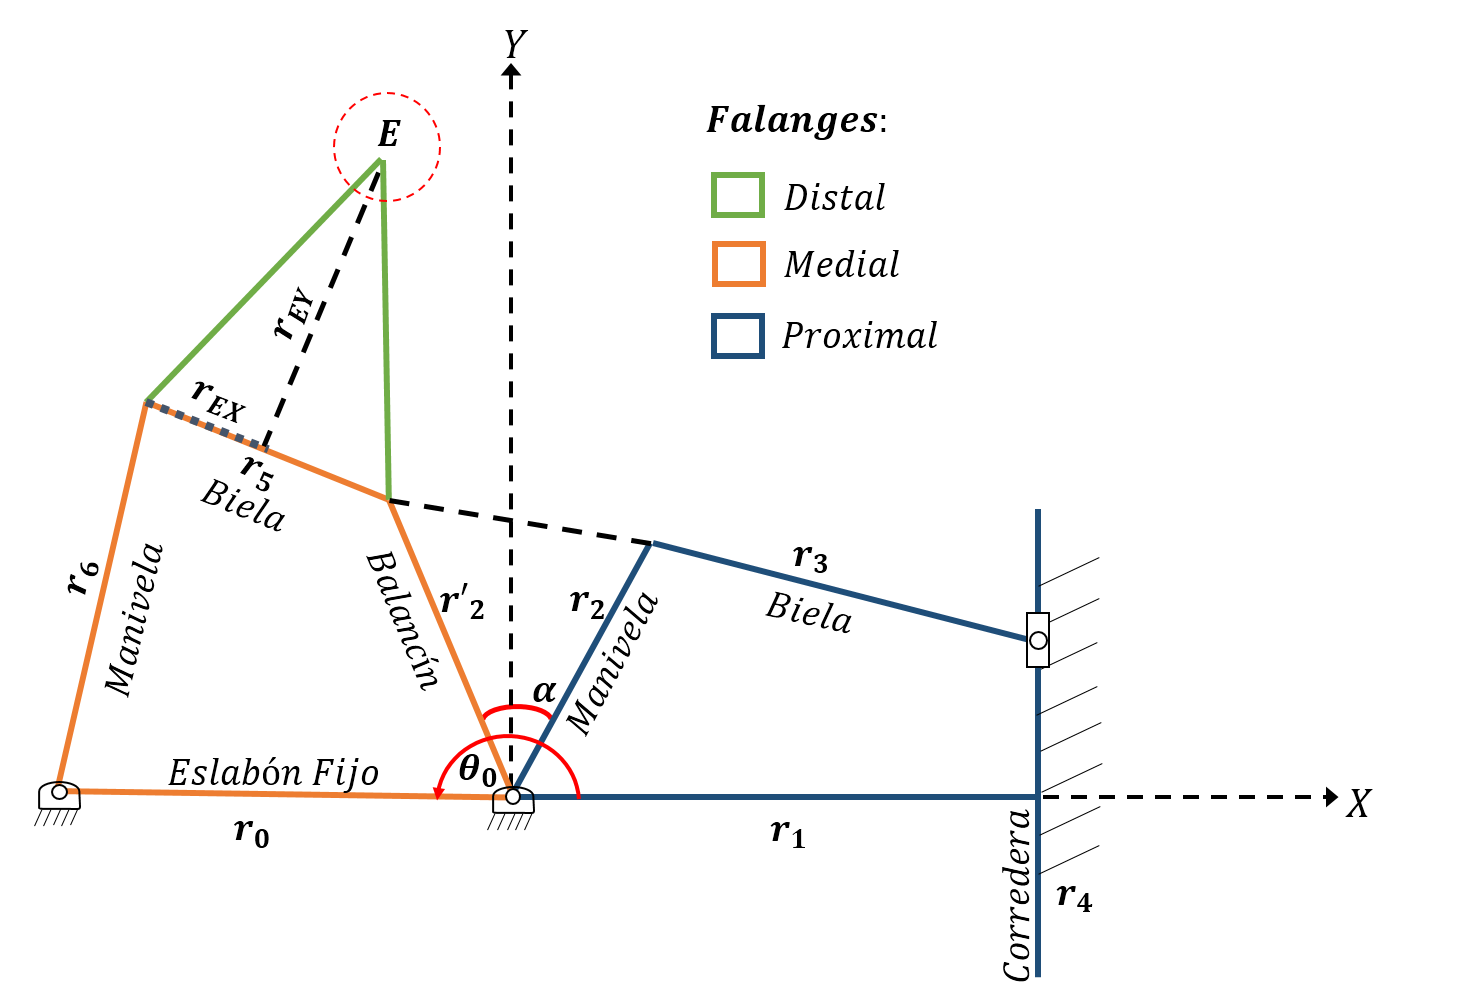
\includegraphics[width=0.9\textwidth]{Griper1.png}
    \caption [Mecanismo de seis barras para el diseño de un dedo del Efector Final.]{Mecanismo de seis barras para el diseño de un dedo del Efector Final. Tomado de \cite{zapata_zapata_control_2017} }
    \label{fig:Griper}
\end{figure}

En la Figura \ref{fig:Griper}, se muestra el diseño de un dedo conformado por dos sub-sistemas que simulan las falanges del mismo. El primer sub-sistema corresponde a un mecanismo manivela-biela-corredera (MBC) que se usa en la entrada ($r_2$, $r_3$, $r_4$), y el segundo es un mecanismo de cuatro barras en la salida ($r_0$, $r^{\prime}_2$, $r_5$, $r_6$). Ambos mecanismos conforman el sistema, en donde el impulsor es la corredera y el punto $E$ en el acoplador es la salida. El análisis de este problema fue tomado del trabajo realizado por Capistrán, Portilla y Mezura en \cite{capistran_2015} y se presenta en la siguiente sección.


\subsection{Cinemática del Efector Final de Tres Dedos }

Para llegar al planteamiento final de este problema de optimización se debe realizar primeramente el análisis de los dos sub-sistemas mencionados en la sección anterior individualmente. Luego, las ecuaciones que describen el comportamiento cinemático de ambos sistemas son integrados para conformar el problema de optimización. Primeramente se analiza el mecanismo MBC (Figura \ref{fig:Griper_MBC}) respecto al eje $X$ según la posición de la corredera $r_4$, en donde se pueden presentar tres casos posibles: $r_4 > 0$, $r_4 < 0$ y $r_4 = 0$. En cada caso la variable de interés que describe al sub-sistema es $\theta_3$. A continuación se presenta el modelo de cada caso \cite{capistran_2015}:
\begin{figure}[htb]
    \centering
     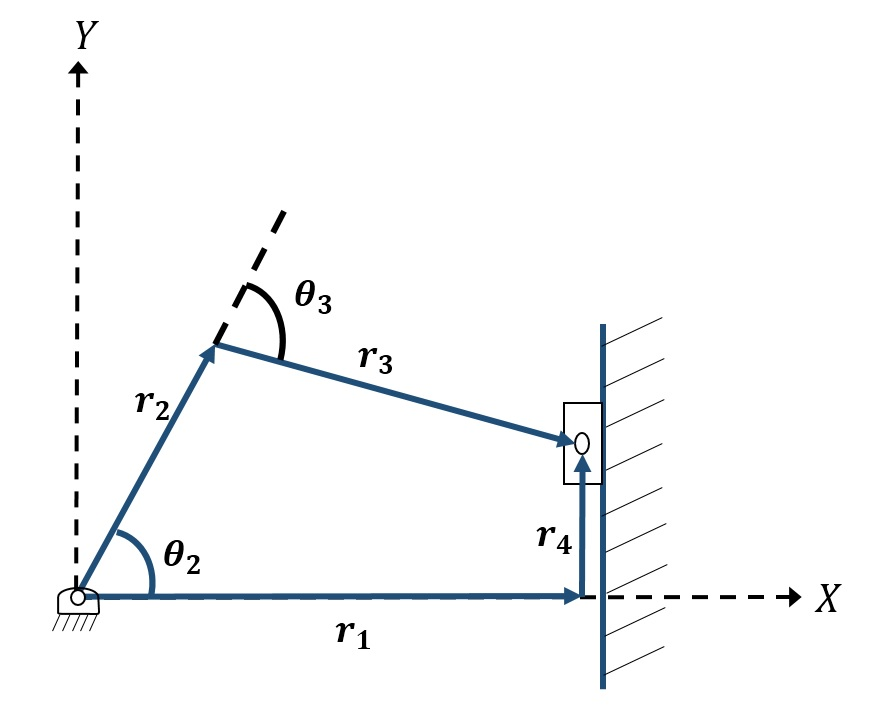
\includegraphics[width=0.8\textwidth]{Griper2.jpg}
    \caption[Mecanismo manivela-biela-corredera en un dedo del Efector Final.]{Mecanismo manivela-biela-corredera en un dedo del Efector Final. Tomado de \cite{zapata_zapata_control_2017} }
    \label{fig:Griper_MBC}
\end{figure}
\begin{enumerate}
\item \textbf{Si} $r_4>0$ \textbf{entonces}:

Se calcula el valor del ángulo $\theta_3$ mediante la sumatoria de los ángulos $\theta_2$, $\varphi$ y $\pi$  (igual a 180). En la Figura \ref{fig:Griper_MBC1} se muestran los ángulos requeridos para efectuar los cálculos necesarios en este caso.
\begin{figure}[htb]
    \centering
     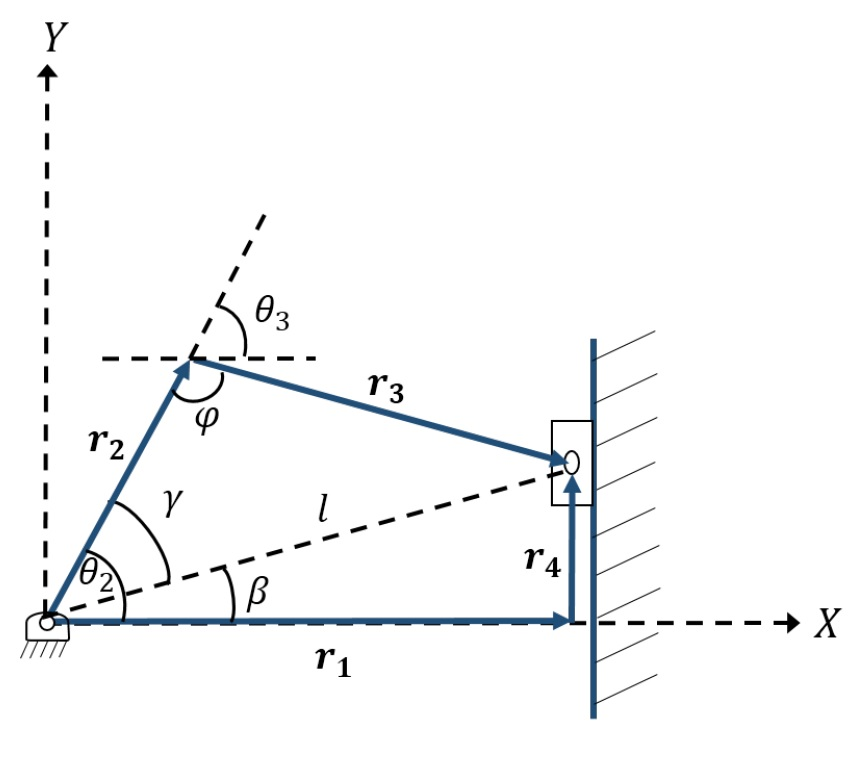
\includegraphics[width=0.8\textwidth]{Griper3.jpg}
    \caption [Mecanismo manivela-biela-corredera para $r_4 > 0$ en un dedo del Efector Final.]{Mecanismo manivela-biela-corredera para $r_4 > 0$ un dedo del el Efector Final. Tomado de \cite{zapata_zapata_control_2017} }
    \label{fig:Griper_MBC1}
\end{figure}

Para calcular $\theta_2$ se procede de la siguiente forma:
\begin{equation}\label{eq:griper_theta2}
\theta_2=\beta+\gamma
\end{equation}
Para obtener $\gamma$ debe calcular $l$ mediante el teorema de pitágoras:
\begin{equation}
l=\sqrt[]{r^2_1 +r^2_4}
\end{equation}
Aplicando la ley de cosenos y despejando se obtiene la Ecuación \ref{eq:griper_gamma} 
\begin{equation} \label{eq:griper_gamma}
\gamma=\cos^{-1}\left[  \frac{r^2_2 +l^2-r^2_3}{2r_2l}\right]
\end{equation}
Para cálculo  del ángulo se plantea que:
\begin{equation}\label{eq:griper_beta} 
\beta=\tan^{-1}\left[  \frac{|r_4|}{r_1}\right]
\end{equation}
Sustituyendo las Ecuaciones \ref{eq:griper_gamma} y \ref{eq:griper_beta} en la Ecuación \ref{eq:griper_theta2} se obtiene:
\begin{equation}\label{eq:griper_theta22}
\theta_2=  \cos^{-1}\left[  \frac{r^2_2 +l^2-r^2_3}{2r_2l}\right]+ \tan^{-1}\left[  \frac{|r_4|}{r_1}\right]
\end{equation}
El valor de $\varphi$ se calcula aplicando ley de cosenos y se despejando:
\begin{equation}\label{eq:griper_varphi}
\varphi=\cos^{-1}\left[ \frac{r^2_2 +r^2_3-l^2}{2r_2r_3}\right]
\end{equation}
Luego, el valor de $\theta_3$ se calcula por la sumatoria expresada en la Ecuación \ref{eq:griper_theta3}
\begin{equation}\label{eq:griper_theta3}
\theta_3=\theta_2+\varphi+\pi
\end{equation}
Esto es:
\begin{equation}\label{eq:griper_theta32}
\theta_3= \cos^{-1}\left[  \frac{r^2_2 +l^2-r^2_3}{2r_2l}\right]+ \tan^{-1}\left[  \frac{|r_4|}{r_1}\right]+\cos^{-1}\left[ \frac{r^2_2 +r^2_3-l^2}{2r_2r_3}\right]+\pi
\end{equation}
%%%%%%%%%%%%%%%%%%%%%%%%%%%

\item \textbf{Si} $r_4<0$ \textbf{entonces}:
\begin{figure}[htb]
    \centering
     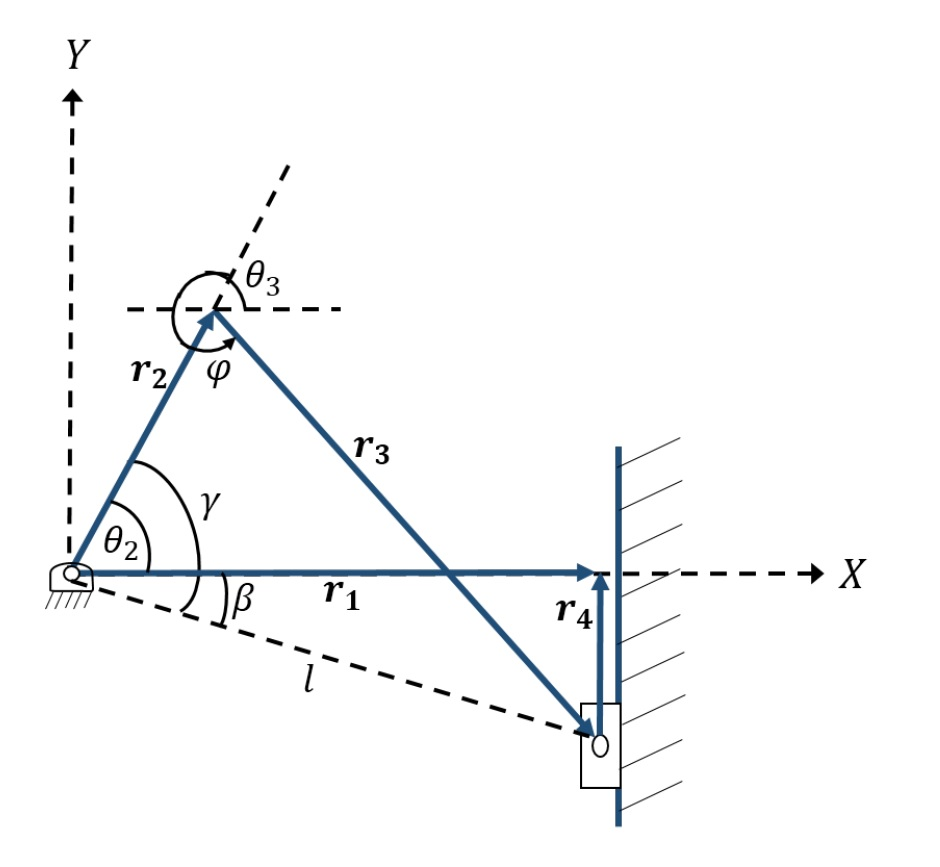
\includegraphics[width=0.8\textwidth]{Griper4.jpg}
    \caption [Mecanismo manivela-biela-corredera para $r_4<0$ en un dedo del Efector Final.]{Mecanismo manivela-biela-corredera para $r_4<0$ en un dedo del Efector Final. Tomado de \cite{zapata_zapata_control_2017} }
    \label{fig:Griper_MBC2}
\end{figure}

El análisis matemático es similar al del caso anterior (Figura \ref{fig:Griper_MBC2}). Se debe calcular el valor del ángulo $\theta_3$ solo que, en este caso el ángulo $\theta_2$ es la diferencia entre los ángulos $\beta$ y $\gamma$:
\begin{equation}\label{eq:griper_theta23}
\theta_2=\beta-\gamma
\end{equation}

Sustituyendo las Ecuaciones \ref{eq:griper_gamma} y \ref{eq:griper_beta} en la Ecuación \ref{eq:griper_theta23} se obtiene:
\begin{equation}\label{eq:griper_theta24}
\theta_2=  \cos^{-1}\left[  \frac{r^2_2 +l^2-r^2_3}{2r_2l}\right]- \tan^{-1}\left[  \frac{|r_4|}{r_1}\right]
\end{equation}

Luego, el valor de $\theta_3$ se obtiene sustituyendo este valor de $\theta_2$  y el valor de $\varphi$ de la Ecuación \ref{eq:griper_varphi},  en la Ecuación \ref{eq:griper_theta3}:
\begin{equation}\label{eq:griper_theta34}
\theta_3= \cos^{-1}\left[  \frac{r^2_2 +l^2-r^2_3}{2r_2l}\right]- \tan^{-1}\left[  \frac{|r_4|}{r_1}\right]+\cos^{-1}\left[ \frac{r^2_2 +r^2_3-l^2}{2r_2r_3}\right]+\pi
\end{equation}
%%%%%%%%%%%%%%%%%%%%%%%%%%

\item \textbf{Si} $r_4=0$ \textbf{entonces}:
\begin{figure}[htb]
    \centering
     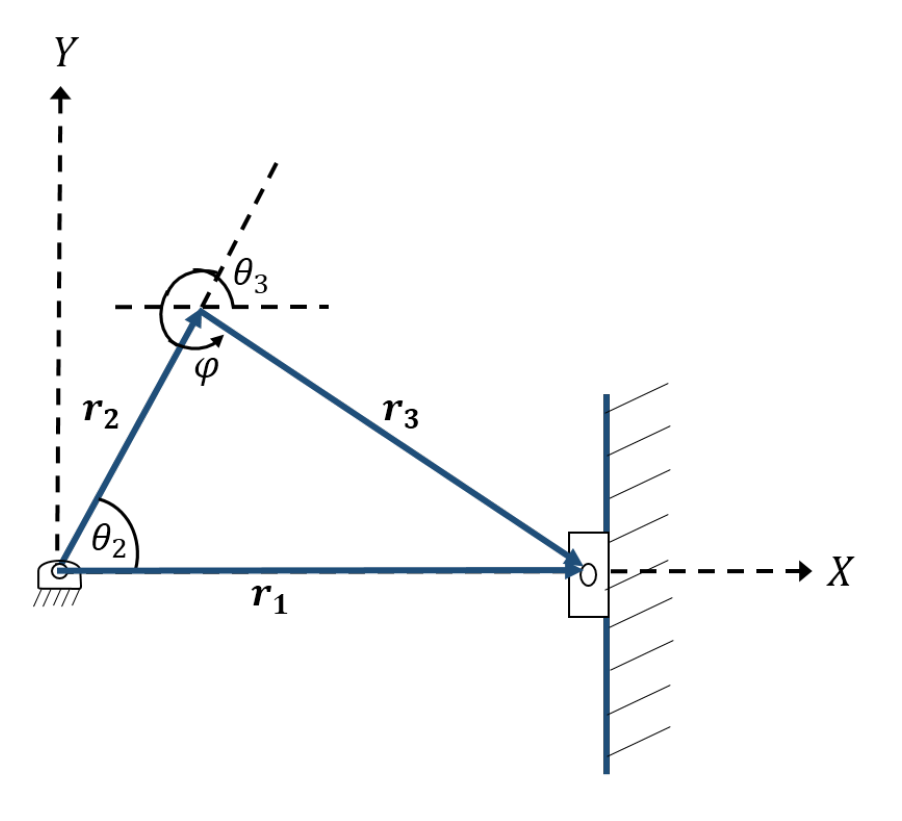
\includegraphics[width=0.8\textwidth]{Griper6.png}
    \caption[Mecanismo manivela-biela-corredera para $r_4 =0$ en un dedo del Efector Final.]{Mecanismo manivela-biela-corredera para $r_4 =0$ en un dedo del Efector Final. Tomado de \cite{zapata_zapata_control_2017} }
    \label{fig:Griper_MBC3}
\end{figure}

En la Figura \ref{fig:Griper_MBC3} se observa que el mecanismo se alinea con el eje $x$ debido a que la corredera $r_4 = 0$. Al igual que en los casos anteriores el valor del ángulo $\theta_3$ es igual a la suma de los ángulos $\theta_2$, $\varphi$ y $\pi$. Para el calculo de $\theta_2$y $\varphi$ se aplica la ley de cosenos y se despeja, obteniendo las Ecuaciones \ref{eq:griper_theta25} y \ref{eq:griper_varphi3}
\begin{equation}\label{eq:griper_theta25}
\theta_2=\cos^{-1}\left[ \frac{r^2_1 +r^2_2-r^2_3}{2r_1r_2}\right]
\end{equation}
\begin{equation}\label{eq:griper_varphi3}
\varphi=\cos^{-1}\left[ \frac{r^2_2 +r^2_3-r^2_1}{2r_2r_3}\right]
\end{equation}
Finalmente, se sustituyen los ángulos $\theta_2$ y $\varphi$  en la Ecuación \ref{eq:griper_theta3}:
\begin{equation}\label{eq:griper_theta33}
\theta_3=\cos^{-1}\left[ \frac{r^2_1 +r^2_2-r^2_3}{2r_1r_2}\right]+\cos^{-1}\left[ \frac{r^2_2 +r^2_3-r^2_1}{2r_2r_3}\right]+\pi
\end{equation}

\end{enumerate}
El análisis cinemático presentado hasta el momento corresponde al sub-sistema MBC del mecanismo de seis barras. A continuación se procede a  desarrollar el modelo cinemático del mecanismo de cuatro barras conformado por los eslabones $r_0$, $r^{\prime}_2$, $r_5$ y $r_6$. En la Figura \ref{fig:Griper_MEC} se muestra dicho mecanismo sin el acoplador. Nótese, que la barra $r_2$ del sub-sistema MBC también forma parte del mecanismo de cuatro barras fungiendo como su impulsor y formando junto con $r^{\prime}_2$ un único eslabón.

\begin{figure}[htb]
    \centering
     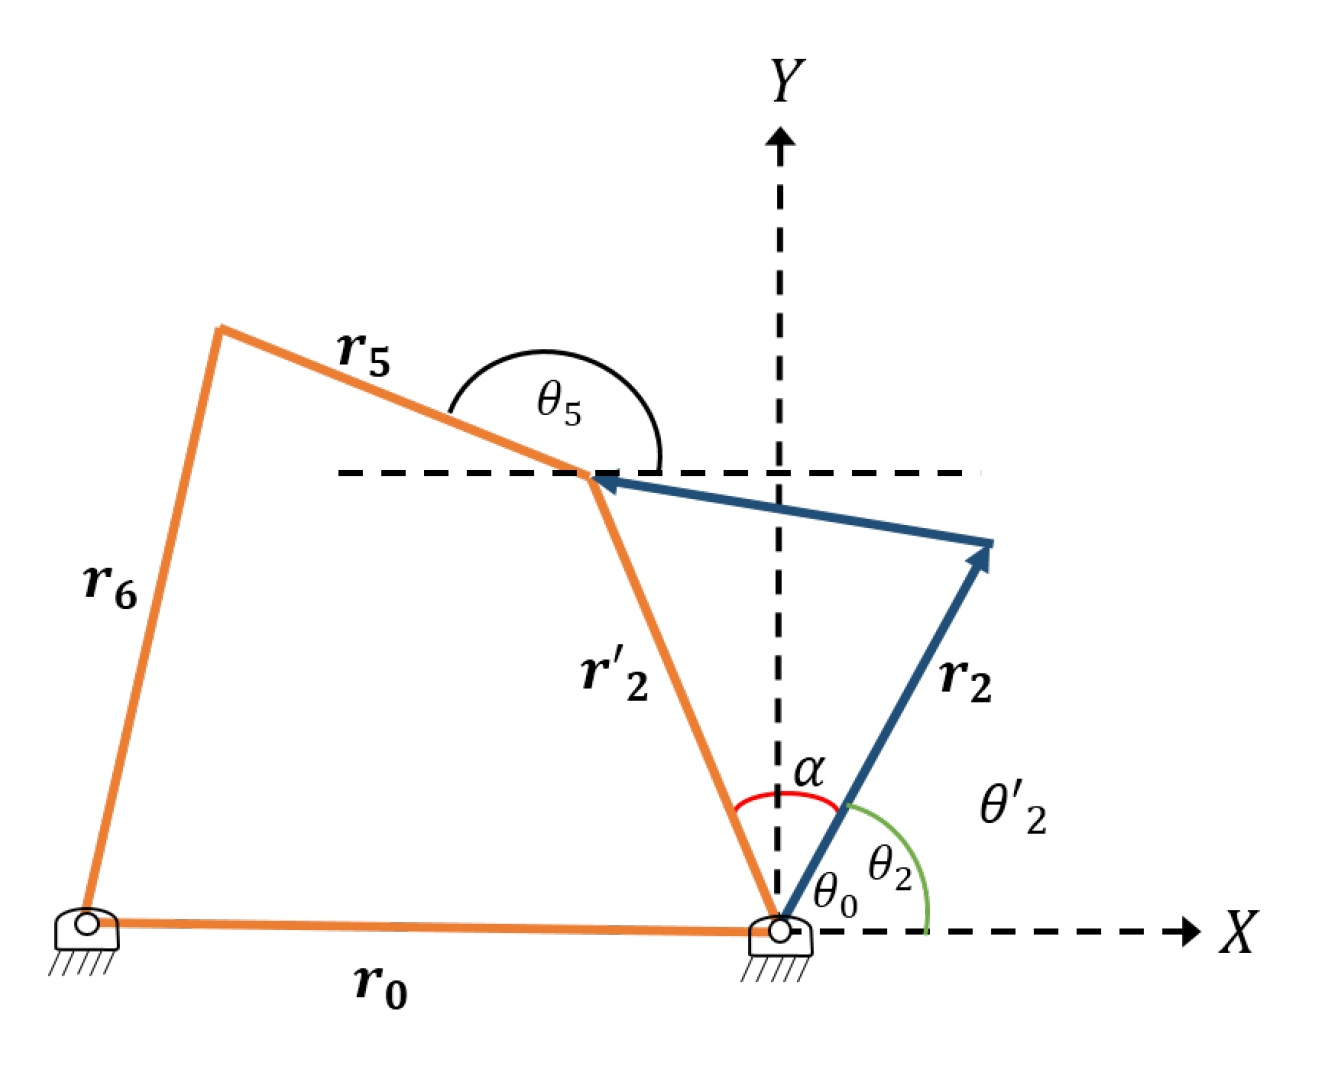
\includegraphics[width=0.8\textwidth]{Griper7.jpg}
    \caption [Mecanismo de cuatro barras de un dedo del Efector Final.]{Mecanismo de cuatro barras de un dedo del Efector Final. Tomado de \cite{zapata_zapata_control_2017} }
    \label{fig:Griper_MEC}
\end{figure}
El análisis cinemático del sub-sistema de cuatro barras es similar al del problema descrito en la Sección \ref{sec:Análisis cinemático de un Mecanismo de Cuatro Barras}. Para iniciar se establece la ecuación de lazo cerrado:
\begin{equation}\label{eq:griper_lazo}
\vec{r^{\prime}_2}+\vec{r_5}=\vec{r_0}+\vec{r_6}
\end{equation}
Utilizando la notación polar se tiene que:
\begin{equation}\label{eq:griper_lazoPolar}
r^{\prime}_2e^{j\theta^{\prime}_2}+r_5e^{j\theta_5}=r_0e^{j\theta_0}+r_6e^{j\theta_6}
\end{equation}
Aplicando la ecuación de Euler y separando la parte real de la parte imaginaria se obtiene:
\begin{eqnarray}
r^{\prime}_2 \cos{\theta^{\prime}_2}+r_5\cos{\theta_4}&=&r_0\cos{\theta_2} +r_6\cos{\theta_6} \label{eq:griper_PolarEuler5} \\
r^{\prime}_2 \sin{\theta^{\prime}_2}+r_5\sin{\theta_4} &=&r_0\sin{\theta_2}+r_6\sin{\theta_6}\label{eq:griper_PolarEuler6}
\end{eqnarray}
en donde:
\begin{equation}
\theta^{\prime}_2=\theta_2+\alpha
\end{equation}
El ángulo $\theta_2$ se obtiene del análisis cinemático del sub-sistema MBC. Luego para calcular $\theta_5$, el sistema de ecuaciones \ref{eq:griper_PolarEuler5} se expresa en función de $\theta_4$ para obtener:
\begin{eqnarray}
r_6\cos{\theta_6}&=& r^{\prime}_2\cos{\theta^{\prime}_2}+r_5\cos{\theta_5}-r_0\cos{\theta_0}\label{eq:griper_PolarEuler7} \\
r_6\sin{\theta_6} &=&r^{\prime}_2\sin{\theta^{\prime}_2}-r_5\sin{\theta_5}r_0\cos{\theta_0}\label{eq:griper_PolarEuler8}
\end{eqnarray}
Se obtiene la ecuación compacta de Freudenstein elevando al cuadrado los términos del sistema de ecuaciones anterior y sumando sus términos:
\begin{equation} \label{eq:griper_A1B1C1}
 A\cos{\theta_3}+B\sin{\theta_3}+C=0 
\end{equation}
Donde:
\begin{eqnarray}
A&=& 2r_5(r^{\prime}_2\cos{\theta^{\prime}_2}-r_0\cos{\theta_0}) \label{eq:griper_A} \\
B&=& 2r_5(r^{\prime}_2\sin{\theta^{\prime}_2}-r_0\sin{\theta_0}) \label{eq:griper_B} \\
C&=& r_0^2+r^{\prime}_2+r_5^2-r_6^2 -2r_0r^{\prime}_2\cos(\theta_0-\theta^{\prime}_2) \label{eq:griper_C}
\end{eqnarray}
El ángulo $\theta_5$ se puede obtener como función de $A$, $B$ y $C$, si $\sen{\theta_5}$ y $\cos{\theta_5}$  se expresan en términos de $\tan(\frac{\theta_5}{2})$:
\begin{eqnarray}
\sin{\theta_5}= \frac{2tan(\frac{\theta_5}{2})}{1+tan^2(\frac{\theta_5}{2})}&,& \cos{\theta_5}= \frac{1-tan^2(\frac{\theta_5}{2})}{1+tan^2(\frac{\theta_5}{2})} \label{eq:griper_enFuncionTheta3}
\end{eqnarray}

Sustituyendo la Ecuación \ref{eq:griper_enFuncionTheta3} en la Ecuación \ref{eq:griper_A1B1C1} se obtiene una ecuación no lineal de segundo orden:
\begin{equation} \label{eq:griper_Lineal2dOrden}
 \left[C-A\right]= tan^2{\frac{\theta_3}{2}}+\left[2B\right]\tan{(\frac{\theta_3}{2})}+A+C=0
\end{equation}
Resolviendo la ecuación \ref{eq:griper_Lineal2dOrden} el ángulo $\theta_3$ puede ser expresado de la siguiente forma:
\begin{equation} \label{eq:griper_noLineal2dOrden_theta5}
\theta_5= 2\arctan \left[ \frac{-B \pm \sqrt{B^2+A^2-C^2}}{C-A} \right]
\end{equation}
El ángulo $\theta_6$ se obtiene de forma similar, siendo la ecuación compacta de Freudenstein:
\begin{equation} \label{eq:griper_A1B1C1_2}
 D\cos{\theta_6}+E\sin{\theta_6}+F=0 
\end{equation}
Donde:
\begin{eqnarray}
D&=& 2r_6(r_0\cos{\theta_0}-r^{\prime}_2\cos{\theta^{\prime}_2}) \label{eq:griper_A_2} \\
E&=& 2r_6(r_0\sin{\theta_0}-r^{\prime}_2\cos{\theta^{\prime}_2}) \label{eq:griper_B_2} \\
F&=& r_0^2+r^{\prime}_2+r_5^2-r_6^2 -2r_0r^{\prime}_2\cos(\theta_0-\theta^{\prime}_2) \label{eq:griper_C_2}
\end{eqnarray}
Luego, $\theta_6$ se define como:
\begin{equation} \label{eq:griper_noLineal2dOrden_theta6}
\theta_6= 2\arctan \left[ \frac{-E \pm \sqrt{E^2+D^2-F^2}}{F-D} \right]
\end{equation}
Las Ecuaciones \ref{eq:griper_noLineal2dOrden_theta5} y \ref{eq:griper_noLineal2dOrden_theta6} determinan los ángulos de la biela y el balancín del mecanismo de cuatro barras. El signo del radical para los ángulos $\theta_5$ y $\theta_6$ también se seleccionan de acuerdo a la la Tabla \ref{tab:Signo del radical} de la Sección \ref{sec:Análisis cinemático de un Mecanismo de Cuatro Barras}. Para analizar, se debe determinar la posición del punto $E$ del acoplador (Figura \ref{fig:Griper_MEC1}) a través de la siguiente relación:
\begin{equation} \label{eq:griper_E}
E=r^{\prime}_2+ r_{EX}+r_{EY}
\end{equation}
En términos de componentes tenemos que:
\begin{eqnarray}
E_{x}&=&r^{\prime}_2\cos{\theta^{\prime}_2} +r_{EX}\cos{\theta_5}+r_{EY}\sin{\theta_{EY}} \label{eq:gripper_Cxr} \\
E_{y}&=&r^{\prime}_2\cos{\theta^{\prime}_2} +r_{EY}\sin{\theta_5}+r_{EY}\cos{\theta_{EY}}\label{eq:gripper_Cyr}
\end{eqnarray}
en donde:
\begin{eqnarray}
\theta^{\prime}_{2} &=& \theta_2-\alpha \\
\theta_{EY} &=& \theta_5-90
\end{eqnarray}

\begin{figure}[htb]
    \centering
     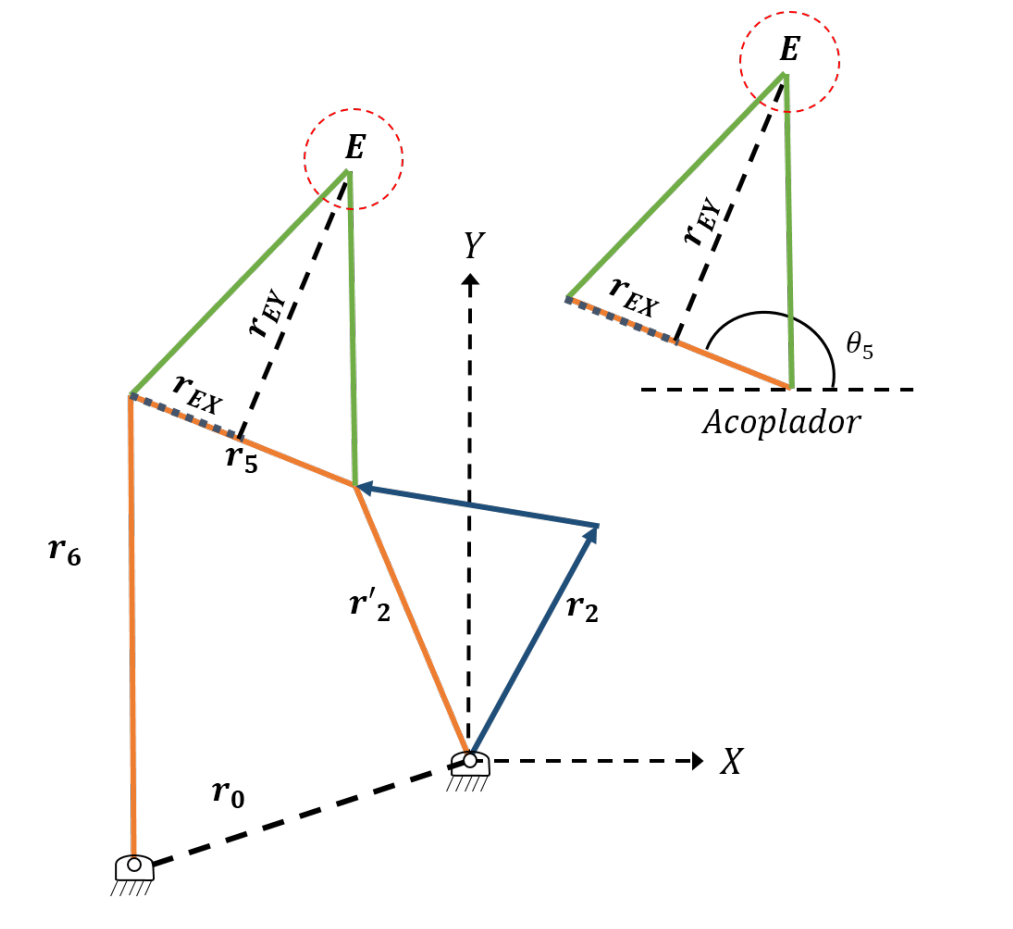
\includegraphics[width=0.8\textwidth]{Griper8.png}
    \caption[Acoplador del mecanismo de cuatro barras en un dedo del Efector Final]{Acoplador del mecanismo de cuatro barras en un dedo del Efector Final. Tomado de \cite{zapata_zapata_control_2017} }
    \label{fig:Griper_MEC1}
\end{figure}
\subsection{Declaración de Problemas de Optimización para Casos de Estudio del Efector}
Para la optimización del diseño correspondiente a un dedo del efector final, se deben encontrar las dimensiones de todas los eslabones del mecanismo de seis barras de tal forma que el punto E del acoplador siga una trayectoria esferica. Los puntos de la trayectoria se encuentran definidos por la Ecuación \ref{eq:griper_puntosP} y fueron tomados de \cite{capistran_2015}.
\begin{equation} \label{eq:griper_puntosP}
 \Omega= \left\{(10, 160), (10, 170), (40, 165) \right\}
\end{equation}
El vector de variables para este caso está constituido por 14 componentes:
\begin{eqnarray}\label{eq:gripper_Vector variables MEC1}
\vec{p} &=& \{p_1,p_2,p_3,...,p_{14} \}\\
       &=& \{ r_1,r_2,r_3,r^1_4,r^2_4,r^3_4,r_0,r^{\prime}_2,r_5,r_6,r_{EX},r_{EY},\alpha,\theta_0 \} 
\end{eqnarray}
En donde $r_1$, $r_2$, $r_3$, $r_0$, $r^{\prime}_2$, $r_5$ y $r_6$ son las dimensiones de las barras. Las variables $r^1_4$,$r^2_4$,$r^3_4$, corresponden a las posiciones de la corredera y se emplean para calcular los puntos en los que se ubica el sistema, $r_{EX}$ y $r_{EY}$ son las dimensiones de las barras del acoplador, mientras que  $\alpha$ es el ángulo entre $r_2$ y $r^{\prime}_2$ , y $\theta_0$ el ángulo de $r_0$.
\subsubsection{Función objetivo}
Para el primer caso del efector final  se plantea la función de error 
\begin{equation}
 \begin{aligned}
min\quad  f(r^i_4)=\sum_{i=1}^{N}\big[\big(C^{i}_{1d}-C^{i} \big)^2=
\sum_{i=1}^{N}\big[\big(C^{i}_{1xd}-C^{i}_{x} \big)^2 +\big(C^{i}_{yd}-C^{i}_{y} \big)^2\big] 
\end{aligned}
\label{eq:gripper_FO}
\end{equation}
En la Ecuación \ref{eq:gripper_FO} se calcula la distancia (a minimizar) de los puntos de precisión $C^i_d$ y los puntos calculados $C_i$ a partir de $r^i_4$. Donde  $C^i_x$ y $C^i$ son las coordenadas $(x,y)$ del punto $E$ del acoplador.
\subsubsection{Restricciones de diseño}\label{sec:Restricciones de diseño MEC_gripper}
Para el correcto funcionamiento del gripper se deben tener en cuenta las siguientes restricciones de diseño: 
\begin{itemize}
\item \textit{Ley de Grashoff:} De forma similar al mecanismo de cuatro barras, debe cumplirse la ley de Grashoff para el mecanismo de seis barras:
\begin{equation}
r_5+r_6 \leq r_0+r^{\prime}_2
\end{equation}
Adicionalmente debe cumplirse que:
\begin{equation}
r_0<r_6, \quad r^{\prime}_2<r_6 ,\quad r_5 < r_6
\end{equation}

\item \textit{Secuencia de posición de la corredera}: Las  posiciones de la corredera deben estar ordenadas de tal forma que cada posición preceda a la siguiente de acuerdo a su magnitud:
\begin{equation}
r^1_4 > r^2_4 > r^3_4
\end{equation}

\item \textit{Consideraciones sobre barras}: Esta restricción tiene como objetivo garantizar un alto nivel en la estética del acoplador. Para lograr ésto $r_{EX}$ debe ser lo más parecida posible a $r_5$, por lo que: 
\begin{equation}
 r_{EX} - r_5 \leq 0
\end{equation}
Además, para el sub-sistema MBC, la relación recomendada entre biela y manivela se encuentra entre $\frac{1}{3}$ y $\frac{1}{5}$, esto es:
\begin{equation}
\frac{1}{5} \leq \frac{r_2}{r_3}\leq \frac{1}{3}
\end{equation}
Luego:
\begin{equation}
r_2 -\frac{r_3}{3} \leq 0 \quad , \quad \frac{r_3}{5} -r_2 \leq 0
\end{equation}
\end{itemize}

Finalmente, se formulan en las siguientes secciones dos casos de estudio para  el diseño óptimo del gripper, ambos comparten el mismo vector de variables y el conjunto de puntos de precisión.
\subsection{Caso de estudio 1: Diseño sin normalización de barras -GCE1}

El problema de optimización mono-objetivo para el este caso de estudio se define como:
 \begin{equation}\label{eq:gripper_FO1}
 \begin{aligned}
min\quad  f(\vec{p})=
\sum_{i=1}^{3}\big[\big(C^{i}_{xd}-C^{i}_{x} \big)^2 +\big(C^{i}_{yd}-C^{i}_{y} \big)^2\big]
\\
\vec{p} \in  {\rm I\!R}^{15}
\\
\end{aligned}
\end{equation}
%1 () =  ⃗ 1 + 2 − 3 − 4 ≤ 0,
Sujeto a:
\begin{eqnarray}\label{eq:Restricciones gripper1}
g_{1}(\vec{p})&=&p_{10}+ p_{9}-p_{8}-p_{7} \leq 0,\\
g_{2}(\vec{p})&=&p_{7}-p_{10} \leq 0,\\
g_{3}(\vec{p})&=&p_{8}-p_{10} \leq 0,\\
g_{4}(\vec{p})&=&p_{9}-p_{10} \leq 0,\\
g_{5}(\vec{p})&=&p_{11}-p_{9} \leq 0,\\
g_{6}(\vec{p})&=&|p_{4}|-|p_{5}| \leq 0,\\
g_{7}(\vec{p})&=&|p_{5}|-|p_{6}| \leq 0,\\
g_{8}(\vec{p})&=&p_{2}-\frac{p_3}{3} \leq 0,\\
g_{9}(\vec{p})&=&\frac{p_3}{3}-p_{2} \leq 0
\end{eqnarray}
Los límites superior e inferior de cada variable de diseño son los siguientes:
\begin{eqnarray}\label{eq:limites variables griper1}
p_1,p_2,p_3 & \in & \left[ 0,100\right] \\
p_4,p_5,p_6 & \in & \left[ -50,0\right] \\
p_7,p_8,p_{10},p_{11},p_{12} & \in & \left[ 0,150 \right] \\
p_9 & \in & \left[ 0,50\right] \\
p_{13} & \in & \left[ \frac{\pi}{12},\pi \right] \\
p_{14} & \in & \left[ \frac{3\pi}{4},\frac{5\pi}{4} \right]
\end{eqnarray}
\subsection{Caso de estudio 2: Diseño con normalización de barras - GCE2}

En el segundo caso de estudio se agrega una función de normalización ($f(\vec{x})$) para las barras del mecanismo, con el fin de obtener un diseño  estético y antropomórfico de las falanges del gripper. La función objetivo queda definida de la siguiente forma:
\begin{equation}\label{eq:griper_FOG1}
  f_r= w_1f(\vec{p})+w_2f(\vec{x})
\end{equation}
esto es:
 \begin{eqnarray}\label{}
min\quad  f(\vec{p})&=&
\sum_{i=1}^{3}\big[\big(C^{i}_{xd}-C^{i}_{x} \big)^2 +\big(C^{i}_{yd}-C^{i}_{y} \big)^2\big] \qquad \vec{p} \in  {\rm I\!R}^{14} \\
min\quad  f(\vec{x})&=&\frac{\sqrt[]{\sum^6_{i=1}\sum_{j=1}(x_j-x_i)^2}}{\sqrt[]{\sum^6_{i=1}x^2_i}} \label{eq:griper_NORM}
\end{eqnarray}
%1 () =  ⃗ 1 + 2 − 3 − 4 ≤ 0,
Sujeto a:
\begin{eqnarray}\label{eq:Restricciones griper2}
g_{1}(\vec{p})&=&p_{10}+ p_{9}-p_{8}-p_{7} \leq 0,\\
g_{2}(\vec{p})&=&p_{7}-p_{10} \leq 0,\\
g_{3}(\vec{p})&=&p_{8}-p_{10} \leq 0,\\
g_{4}(\vec{p})&=&p_{9}-p_{10} \leq 0,\\
g_{5}(\vec{p})&=&p_{11}-p_{9} \leq 0,\\
g_{6}(\vec{p})&=&|p_{4}|-|p_{5}| \leq 0,\\
g_{7}(\vec{p})&=&|p_{5}|-|p_{6}| \leq 0,\\
g_{8}(\vec{p})&=&p_{2}-\frac{p_3}{3} \leq 0,\\
g_{9}(\vec{p})&=&\frac{p_3}{3}-p_{2} \leq 0
\end{eqnarray}
Los límites superior e inferior para las variables de diseño son:
\begin{eqnarray}\label{eq:limites variables griper2}
p_1,p_2,p_3 & \in & \left[ 0,100\right] \\
p_4,p_5,p_6 & \in & \left[ -50,0\right] \\
p_7,p_8,p_{10},p_{11},p_{12} & \in & \left[ 0,150 \right] \\
p_9 & \in & \left[ 0,50\right] \\
p_{13} & \in & \left[ \frac{\pi}{12},\pi \right] \\
p_{14} & \in & \left[ \frac{3\pi}{4},\frac{5\pi}{4} \right]
\end{eqnarray}
En la Ecuación \ref{eq:griper_FOG1}, $w_1$ y $w2$ son pesos que controlan la precisión de la trayectoria y la estética del mecanismo, respectivamente. La suma de ambos pesos debe ser igual 1, por lo que, para este caso se tomarán los valores de $w_1=0.9$ y $w_2=0.1$. Las variables $x_i$ y $x_j$ de la Ecuación \ref{eq:griper_NORM} están relacionadas con las coordenadas de cada barra del sistema.

\section{Gestión de Generación de Energía en una Microrred Eléctrica}
En la actualidad los sistemas de generación y distribución de energía convencionales enfrentan diversos problemas como el agotamiento gradual de los recursos de combustibles fósiles, la escasa eficiencia energética y la contaminación ambiental. Estos problemas han impulsado la tendencia de generar energía localmente mediante el uso de \textit{Fuentes de Energía Renovables} (FER) como gas natural, biogás, energía eólica, panales solares fotovoltaicos, sistemas combinados de calor y energía, y su integración en la red de distribución energía de uso público. Este tipo de generación de energía se denomina \textit{generación distribuida} (GD) y las fuentes de energía se denominan\textit{ recursos de energía distribuida }(RED). El término generación distribuida se utiliza para distinguir este concepto de generación convencional centralizada. Debido al aumento tanto de la demanda de energía eléctrica como del uso las FER, la utilización de microrredes eléctricas ha tenido un aumento en las ultimas décadas. Lasseter plantea lo siguiente en  \cite{lasseter2002microgrids}:
\begin{quote}
\textit{``Las microrredes son redes de suministro de energía de pequeña escala, diseñadas para suministrar cargas eléctricas o térmicas a una comunidad pequeña, como una urbanización o una localidad suburbana. Una Microrred es esencialmente una red de distribución ya que es un conglomerado de sistemas GD con diferentes cargas a nivel de voltaje de distribución. Los generadores o micro-fuentes empleados en una Microrred suelen ser de Generación Distribuida renovable o no convencional."}
\end{quote}


Desde el punto de vista operativo, las micro-fuentes deben estar equipadas con interfaces electrónicas de potencia (IEP) y controles para proporcionar la flexibilidad requerida y  garantizar así el funcionamiento como sistema único. Esta flexibilidad de control permite que la microrred se presente al sistema de energía de la red principal como una sola unidad controlada que satisface las necesidades locales de energía. La principal ventaja de una microrred es su facilidad de control, así como el cumplimiento de las regulaciones de la red sin obstaculizar la confiabilidad y seguridad del servicio eléctrico. Desde el punto de vista de los clientes, las microrredes son beneficiosas para satisfacer localmente sus requisitos eléctricos. También pueden suministrar energía ininterrumpible, mejorar la confiabilidad local y proporcionar soporte de voltaje local. Desde el punto de vista ambiental, las microrredes reducen la contaminación ambiental y el calentamiento global mediante la utilización de tecnología que produce bajas emisiones de carbono  \cite{lasseter2002microgrids}. 

Sin embargo, para lograr una operación estable y segura mediante micro-redes, es necesario resolver una serie de problemas técnicos, normativos y económicos. Ciertas características de las microrredes pueden resultar problemáticas. Algunas intrínsecas, como la naturaleza intermitente y dependiente del clima de la generación mediante ciertos tipos de FER como la fotovoltaica y la eólica; u otras como el bajo contenido de energía de los combustibles no fósiles, la falta de estándares y regulaciones para operar las microrredes de forma factible. El estudio de estas cuestiones requiere un amplio análisis en tiempo real y en simulaciones, que ha sido objeto de diferentes investigaciones.

 \subsection{Optimización del costo de la generación de energía en una Microrred Eléctrica No Interconectable - SCE1}
En el presente problema el objetivo es minimizar el costo de operación de una  Microrred Eléctrica en un lugar Remoto no Interconectable (MR-RNI), al tiempo que se garantiza el equilibrio entre la generación y la demanda. La generación fiable de energía se logra mediante la generación híbrida de potencia en donde se emplean FER, generación convencional con diésel y Sistemas de Almacenamiento de Energía (SAE). Las variables de diseño representan entonces, las potencias que serán suministradas por los Generadores de Diésel (GD), energía fotovoltáica (GFV), energía eólica (GE) y el  de la MR-RNI en función del tiempo dentro de un intervalo de 24 horas. Se define un modelo de optimización basado en el despacho económico, el cual intenta obtener el menor costo posible derivado del uso del sistema, mientras los generadores entregan potencia a la carga total. El cálculo de minimización del costo de la generación de energía  eléctrica en la MR-RNI se debe realizar para un periodo de 24, donde cada hora del día representa un problema de optimización con límites para las variables de diseño diferentes en cada hora. Esto se debe a que los recursos para la generación diaria son variables. Específicamente debe tomarse en cuenta los siguientes escenarios \cite{zapata_zapata_control_2017}: 
\begin{enumerate}
\item Las FER no pueden entregar energía las 24 horas.
\item La demanda total de energía no puede ser entregada solo por las FER.
\item Los costos más representativos son los de combustible,y por tanto la potencia entregada por el generador de diésel es la más costosa.
\item La operación de los sistemas de generación híbrida de potencia tiene un costo generalmente no lineal.
\end{enumerate}
\subsubsection{Costo de Generación Diésel}
La GD presenta una función de costo asociada a la potencia del generador. Dicha función se encuentra dada por la Ecuación \ref{eq:GD}, en donde $i$ es la $i$-ésima fuente de generación , $P_i$ y $F_i$ son la salida de potencia eléctrica y el costo de operación de la fuente $i$, respectivamente, mientras que $\alpha$, $\beta$  y $\gamma$ son los cocientes de costo.
 \begin{equation}\label{eq:GD}
   f(P_i)=\alpha_i +\beta_iP_i +\gamma P^2_i
 \end{equation}
Para  $\alpha=14.88$, $\beta=0.3$  y $\gamma=0.000435$ según se plantea en \cite{zapata_zapata_control_2017}. Luego la función de costo correspondiente a la generación de diésel se define entonces como:
 \begin{equation}\label{eq:GD1}
   f_1(P_1)=14.88 +0.3P_1 +0.000435 P^2_1
 \end{equation}

\subsubsection{Costo de Generación Solar Fotovoltaica}
Para el generador de energía fotovoltaica se define la siguiente función de costo de generación:
\begin{equation}\label{eq:PV1}
   f_3(P_3)=\alpha I^p P_3 +G^EP_3 
 \end{equation}
 
 \begin{equation}\label{eq:PV2}
  \alpha = \frac{r}{\left[1+(1+r)^{-N}\right]}
 \end{equation}

En este caso $P_3$ es la potencia de salida de GFV, $\alpha$ es la tasa de retorno de inversión y $r$ corresponde a la tasa de interés (se considera de 0.09 para el caso base), $N$ es la vida útil del generador, que ha sido establecida
en 20 años, $I^p$ indica el costo de inversión por unidad de potencia (\$5000=kW) y $G^E$ es el costo de operación y mantenimiento por unidad de potencia generada. La función de costo por generación fotovoltaica queda definida entonces como:
\begin{equation}\label{eq:PV3}
   f_3(P_3)=545.016P_3 
\end{equation}
\subsubsection{Costo de Generación de Energía Eólica}
Según lo planteado en \cite{zapata_zapata_control_2017} se toman los mismos
valores de $I^p$ y $G^E$, la función de costo para la generación eólica queda como:
\begin{equation}\label{eq:GE}
f_4(P_4) = 152.616P_4
\end{equation}
\subsubsection{Costo de Sistema de Almacenamiento de Energía}
Para el SAE se considera un banco de baterías de 2kW. En \cite{zapata_zapata_control_2017}, el costo $I^p$ por unidad de almacenamiento instalada es de \$1000/kW, mientras que el $G^E$ es igual a \cent 1.6/kW y representa el costo de operación y mantenimiento por unidad de potencia generada. El uso del SAE describe la siguiente función de costo:
\begin{equation}\label{eq:ESS}
f_2(P_2) = 119P_2
\end{equation}
\subsection{Planteamiento del Problema de Optimización}
El despacho económico es un método eficiente para obtener un menor costo del sistema al tiempo que se satisface la carga o demanda de energía mediante el despacho de las fuentes de generación. Simultáneamente, las restricciones de las fuentes de generación deben ser satisfechas. En el presente caso de estudio se deben calcular las potencias de cada uno de los generadores en la MR-RNI en cada hora del día, minimizando el costo. El vector de variables de diseño se plantea en la Ecuación  \ref{eq:MR-vector de variables}:
 \begin{equation}\label{eq:MR-vector de variables}
  \vec{p}=\left[ P_1,P_2,P_3,P_4 \right]^T
 \end{equation}


La formulación clásica del despacho económico se plantea en \cite{Ramabhotla_Economic_dispatch} de la siguiente forma:
 \begin{equation}
 min\quad  F=
 \sum_{i=1}^{NG}F_{i}P_{i} 
 \end{equation}

Donde $NG$ es el número de fuentes; $P_{i}$ es el generador de fuente $i$; $F_{i}$ es el costo total de producción de la fuente $i$. Luego la función objetivo considerada para el caso de estudio en cuestión tiene en cuenta la variabilidad de la carga en cada hora  $\tau$ del día según la Ecuación \ref{eq:MR-FO}
 \begin{equation}\label{eq:MR-FO}
min \quad f(\vec{p} ) = w_1C_f f(P_1(\tau)) + w_2f(P_2(\tau)) + w_3f(P_3(\tau))+ w_4f(P_4(\tau))
 \end{equation}
 
Donde $w_1$, $w_2$, $w_3$, $w_4$ son los pesos asignados a los generadores, cumpliéndose que  $w_1+ w_2+w_3+w_4=1$ y  se establece que $w_1=w_2=w_3=w_4=0.25$. $C_f$ es el costo del combustible de diésel que se asignó en 1 USD.


Teniendo en cuenta que el costo de generación de energía debe ser calculado en cada hora del día la función objetivo para las 24 horas del día se define según la Ecuación \ref{eq:MR-FO2}:
\begin{equation}\label{eq:MR-FO2}
 min\quad  F=
 \sum_{\tau=1}^{24}f(\vec{p}_\tau) \quad \vec{p}_\tau \in {\rm I\!R}^{4}
 \end{equation}
\subsubsection{Restricciones de Diseño}
La gestión de generación de energía en la MR-RNI está sujeta a las siguientes restricciones de diseño:
\begin{itemize}
\item \textit{Balance de potencia}: La suma de las potencias suministradas por los cuatro generadores debe ser igual a la carga $P_L$ del sistema :
 \begin{equation}
P_1+P_2+P_3+P_4=P_L
 \end{equation}
 \item \textit{Modelo del banco de baterías}: El poder de salida del generador PV y la carga demandada en cierta hora $t$, determinan el poder de carga y descarga dentro y fuera del banco de baterías.
El estado de carga ($SOC$ por sus siglas en inglés) del banco de baterías en cualquier hora, $SOC(t)$,depende del $SOC$ en la hora previa $SOC(t-1)$. Luego, para el flujo de energía de la hora $t-1$ a $t$, se debe considerar la siguiente relación \cite{tazvinga2013minimum}:
 \begin{equation}
SOC(t)=SOC(t-1)- \alpha_DP_2(t)+\alpha_CP_3(t)+\alpha_CP_4(t)
 \end{equation}
 Donde $\alpha_D=\frac{\eta_D}{Bc_{max}}$, $\alpha_C=\frac{\eta_C}{Bc_{max}}$ y $\eta_D$ y $\eta_D$ son las eficiencias de carga y descarga del banco de baterías respectivamente. Luego la expresión que describe la dinámica de la batería se define como \cite{tazvinga2013minimum}:
  \begin{equation}
SOC(t-1)=SOC(0)- \alpha_D \sum_{\tau=1}^{t}P_2(\tau)+\alpha_C\sum_{\tau=1}^{t}P_3(\tau)+\alpha_C \sum_{\tau=1}^{t}P_4(\tau)
 \end{equation}
 
donde se tiene que $SOC(0)$ como el $SOC$ inicial de la batería y  $\alpha_C\sum_{\tau=1}^{t}P_3(\tau)+\alpha_C \sum_{\tau=1}^{t}P_4(\tau)$ es el poder aceptado por la batería en la hora $t$ y  $\alpha_D \sum_{\tau=1}^{t}P_2(\tau)$ es el poder de descarga de la batería en el tiempo $t$.
Además se debe tener en cuenta que la capacidad disponible de la batería no debe ser menor que la capacidad mínima permitida ni mayor que la capacidad máxima permitida \cite{tazvinga2013minimum}, es decir:
\begin{equation}
SOC^{min}-SOC(t)\leq 0 \quad, \quad SOC(t)-SOC^{max}-\leq 0 
 \end{equation}
 Los parámetros del banco de baterías se muestran en la Tabla \ref{tab:MR-Parámetros del Sistemas de Almacenamiento de Energía}
\begin{table}[]
\centering
\begin{tabular}{ll}
\hline
 Parámetros &   \% \\ \hline
 Eficiencia de carga ($\eta_C$)  & 85 \\
 Eficiencia de descarga ($\eta_D$) & 100  \\
 Estado máximo de carga ($SOC_{max}$)& 95\\ 
 Estado mínimo de carga ($SOC_{min}$)& 40\\
 \hline
\end{tabular}
\caption{Parámetros del Sistemas de Almacenamiento de Energía en la Micro-Red No Interconectable.}
\label{tab:MR-Parámetros del Sistemas de Almacenamiento de Energía}
\end{table}

\end{itemize}
Teniendo en cuenta las secciones anteriores, se plantea el problema de optimización mono-objetivo para el caso de estudio de la MR-RNI descrito por las Ecuaciones de la \ref{eq:MR-FO3} a la \ref{eq:ultima restriccion MR}:

\begin{equation}\label{eq:MR-FO3}
 min\quad  F=
 \sum_{\tau=1}^{24}f(\vec{p}_\tau) \quad \vec{p}_\tau \in {\rm I\!R}^{4}
 \end{equation}
 Sujeto a:
\begin{eqnarray}\label{eq:Restricciones MR}
g_1(\vec{p}_\tau)&=&P_1(\tau)+P_2(\tau)+P_3(\tau)+P_4(\tau)=P_L(\tau)\\
g_2(\vec{p}_\tau)&=&SOC^{min}-SOC(t)\leq 0 \\
g_3(\vec{p}_\tau)&=&SOC(t)-SOC^{max}-\leq 0 
\end{eqnarray}
La carga $P_L(\tau)$ fue obtenida de \cite{tazvinga2014energy} y los límites superior e inferior de cada variable se encuentran definidos como:
\begin{eqnarray}\label{eq:Restricciones MR3}
0  & \leq & P_1(\tau)   \leq  GD_{nominal} \\
0  & \leq & P_2(\tau)   \leq  SOC(0) \times Bc_{max}-  SOC^{min} \times  Bc_{max}\\
0  & \leq & P_3(\tau)   \leq  P_{pv}( \tau) \\
0  & \leq & P_4(\tau)   \leq  P_{wind}(\tau )  \label{eq:ultima restriccion MR}
\end{eqnarray}
donde $GD_{nominal}$ es la capacidad nominal del generador diésel, con un valor de 5000 VA (5 kVA) para cada hora del día en este caso de estudio. El límite superior para $ P_2(\tau)$ depende de la capacidad máxima de la batería ($Bc_{max}$) que es de 2000 VA (2 kVA) y el estado inicial de la misma. Los datos de $ P_{pv}( \tau)$ y $ P_{wind}(\tau )$  fueron tomados de \cite{Ramabhotla_Economic_dispatch}. El estado de carga $SOC(0)$ de la batería se generó de forma aleatoria entre un rango de 40\% y 95\%. La potencia de $P_3$ es equivalente a siete módulos fotovoltaicos.				
	
						


\section{Conclusiones del capítulo}
En el presente capítulo se plantea la formulación matemática de los problemas a resolver por la propuesta de solución. Es necesario primeramente destacar la complejidad de los diferentes casos de diseño cinemático de mecanismos, donde el análisis realizado para obtener la trayectoria deseada por el punto del acoplador, concibe una función compleja no lineal que incluye operaciones mediante funciones trigonométricas y de potencias sobre las variables de diseño. Se puede observar que la función objetivo de estos problemas puede tener valores imaginarios (Ecuación \ref{eq:MEPolarEuler}) para vectores reales. Al no estar definida en los reales para todo su dominio, los métodos de optimización basados en información del gradiente suelen no ser aplicables, surgiendo la necesidad de aplicar métodos directos. Además, las restricciones de diseño para garantizar el cumplimiento de las leyes de Grashoff y la secuencia de ángulos acotan el espacio factible aumentando la dificultad del problema. 

A diferencia de los casos de diseño de mecanismos, la función objetivo a optimizar en el problema de la MR-RNI es una función cuadrática. Sin embargo, en este problema se presentan límites diferentes en cada hora del día para las variables de diseño. Para la potencia generada por el sistema de almacenamiento de energía, este límite depende del estado de la carga en la hora anterior lo que representa un reto para el algoritmo de optimización. Por otra parte, el balance de carga implica una restricción de igualdad, las cuales son generalmente más difíciles de satisfacer.  
\chapter{Hibridación de Métodos de Programación Matemática con Algoritmos Evolutivos} \label{Chapter6} 


En los Capítulos \ref{Chapter3} y \ref{Chapter4} se presentan dos esquemas importantes en cuanto al diseño de algoritmos en el área de la optimización, específicamente en la optimización de problemas con espacios de búsqueda continuos. En el primer esquema se tienen los algoritmos clásicos de programación matemática los cuales son eficientes buscadores locales, y  en el segundo se encuentran algoritmos evolutivos, los cuales utilizan una población de individuos (soluciones candidatas) que les permite obtener información global sobre el espacio de búsqueda. Teniendo en cuenta estos dos esquemas, este capítulo describe la propuesta de solución diseñada durante la presente investigación.

La calidad del desempeño de un algoritmo de optimización depende en gran medida del balance entre las operaciones de exploración y explotación del espacio de búsqueda que sean concebidas en su diseño. Cuando los operadores del algoritmo están orientados a la explotación, este puede quedar estancado en mínimos locales o bien ser sensible al punto de inicio debido a que sólo se conoce una región limitada del espacio de posibles soluciones. Sin embargo, los algoritmos con estas características presentan una mayor velocidad de convergencia al mínimo para espacios de búsqueda convexos. Por otra parte, un algoritmo con operadores mayormente exploratorios presentará generalmente una convergencia lenta y tiempos de ejecución altos; pero no será sensible al punto de inicio y la probabilidad de quedar estancado en mínimos locales será menor.

Debido a la diversidad de problemas en el área de la optimización este balance es difícil de lograr. Algunos problemas requerirán mayor explotación en regiones prometedoras para agilizar la búsqueda, y en otros se necesitará información global del espacio de búsqueda (operaciones de exploración) para encontrar la solución óptima. Esta cuestión es abordada en los teoremas de No Free Lunch para la optimización, donde se plantea que si un algoritmo se desempeña particularmente bien en promedio para una clase de problemas, entonces debe hacerlo peor en promedio con respecto a los problemas restantes. En particular, si un algoritmo tiene mejor rendimiento que la búsqueda aleatoria en una clase de problemas, entonces debe tener un rendimiento peor que la búsqueda aleatoria en las clases de problemas restantes \cite{wolpert1997no}. En este sentido la hibridación puede resultar un enfoque efectivo para diseño de algoritmos más eficientes y que puedan resolver eficazmente un amplio espectro de problemas.

En el contexto de las metaheurísticas, la hibridación se refiere principalmente al proceso de combinar o integrar las mejores características de dos o más algoritmos, para formar uno nuevo que supere las partes originales en la resolución de un problema específico o un conjunto de problemas de referencia general \cite{Swagatam_2011}. Dragoi en \cite{Dragoi_2015} considera tres clasificaciones de hibridación de acuerdo a diferentes aspectos.
\begin{enumerate}
\item  Según los tipos de algoritmos que participan en la hibridación:
\begin{enumerate}
\item Metaheurísticas con metaheurísticas.
\item Metaheurísticas con algoritmos específicos del problema.
\item Metaheurísticas con métodos de programación matemática o inteligencia artificial (que, a su vez, pueden ser: técnicas exactas u otras heurísticas)
\end{enumerate}

\item Con respecto al nivel de hibridación, se encuentran dos casos:
\begin{enumerate}
\item Acoplamiento débil de alto nivel (los algoritmos conservan sus propias identidades)
\item Acoplamiento fuerte de bajo nivel (se intercambian componentes individuales)
\end{enumerate}

\item Cuando se toma en cuenta el orden de ejecución, la hibridación puede ser: 
\begin{enumerate}
\item  Secuencial.
\item  Intercalada.
\item  Paralela
\end{enumerate}
\end{enumerate}
De las siguientes clasificaciones se infiere la diversidad de investigaciones en el área de la hibridación. A continuación se presentan algunos trabajos de hibridación desde el enfoque que concibe una metaheurística como buscador global y un método directo de programación matemática como buscador local. Específicamente se destacarán los trabajos previos que se presentan los dos algoritmos utilizados en la propuesta de solución la Evolución Diferencial (buscador global) y el método de Nelder Mead como buscador local.
%%%%%%%%%%%%%%%%%%%%%%%%%%%%%%%%%%%%%%%%%%%%%%%%%%%%%%%%%%%%%%%%%%%%%%%%%%%%%%%%

\section{Hibridación de la Evolución Diferencial con Métodos de Búsqueda Local}

En el capítulo introductorio del presente trabajo se abordó el concepto de algoritmo memético (AM): un esquema que utiliza una metaheurística como algoritmo base de búsqueda global y que aplica métodos de búsqueda local para mejorar el rendimiento y refinar a los individuos en la población. Este tipo de hibridación es un enfoque integrador (coercitivo), ya que el algoritmo de búsqueda local se considera un subordinado y está incorporado en otro algoritmo \cite{raidl2006unified}. Diversos estudios muestran que, para algunos problemas, los AM son más eficientes y más efectivos que los AE tradicionales \cite{krasnogor2005tutorial}. Los trabajos de hibridación más destacados que combinan la ED y un método de programación matemática se encuentran dentro de este tipo de esquema y sirvieron como base para el enfoque propuesto.

En el artículo ``Algoritmo Integrado de Estrategias de Evolución Diferencial con Búsqueda Local''  (ISDE-L), se aplica un procedimiento de búsqueda local para mejorar el rendimiento \cite{elsayed2011integrated}. En en cada $k$ generaciones, se ordena la población según su valor de aptitud y se selecciona un individuo al azar del 25\% de la población. A este individuo se le aplica una técnica de búsqueda local con un número máximo de evaluaciones. La búsqueda local consiste en elegir aleatoriamente una variable del vector seleccionado, y luego se le suma o resta un número gaussiano aleatorio, como un tamaño de paso, tomándose la mejor dirección de acuerdo con la función de aptitud. Si el paso es exitoso y  mejora el individuo seleccionado, entonces el valor se actualiza. Este proceso continúa hasta que se seleccionan todas las variables o se alcanza el número máximo de evaluaciones. El algoritmo ISDE-L es aplicado al conjunto de problemas de prueba presentados en congreso CEC 2010. Los resultados obtenidos fueron mejores o iguales a los alcanzados por algoritmos de vanguardia para estos problemas prueba.

 Liao en \cite{liao2010two}, combina una versión de la ED modificada (MDE) con el método de Caminata Aleatoria con Dirección de Explotación (RWDE por sus siglas en inglés) como el operador de búsqueda local para mejorar los vectores $x_{r_1}$,$x_{r_2}$ y $x_{r_3}$ en la mutación diferencial. RWDE es un método iterativo de optimización estocástica que genera una secuencia de aproximaciones al óptimo al asumir un vector aleatorio como una dirección de búsqueda. El algoritmo híbrido resultante es llamado MDE-LS ( del inglés Modified Differential Evolution- Local Search) y es considerado por el autor como un algoritmo memético. Se seleccionan un total de catorce problemas de diseño de ingeniería encontrados en literatura en diferentes campos de ingeniería. En siete de los catorce problemas, el algoritmo MDE-LS encuentra el óptimo global dentro del error 10E-6 en treinta ejecuciones. El algoritmo MDE-LS produce tasas de éxito más altas en 8 problemas pero menor en 2, en comparación con las del algoritmo MDE. En general, el MDE-LS mejora la tasa de éxito promedio en un 10\% sobre el algoritmo MDE.



En \cite{neri2008memetic}, se presenta una algoritmo memético que utiliza como buscador global la ED y dos algoritmos de búsqueda local, el Algoritmo Hooke-Jeeves (HJ) y el Buscador Local Estocástico (SLS por sus siglas en inglés). Los métodos de búsqueda local ayudan al marco evolutivo (ED) al ofrecer perspectivas exploratorias alternativas. El objetivo de ambos algoritmos es mejorar localmente una solución inicial explorando su vecindad. El espacio a explorar por los buscadores locales tiene un radio inicial. Luego, cuando no es posible  realizar una mejora, se genera una vecindad del espacio más pequeña reduciendo el radio. Para ambos algoritmos de búsqueda local, se establece un presupuesto igual a 300 evaluaciones de la función de aptitud. Los resultados estadísticos muestran los MA presentados son competitivos con la ED y no requieren un ajuste de parámetros que podría terminar siendo costoso en términos de recursos de cómputo. 

Rogalsky y Derksen en \cite{rogalsky2000hybridization} proponen un algoritmo híbrido que combina el método el descenso simple (DS) con la ED para de acelerar la convergencia del algoritmo, sin que este quede atrapado en los mínimos locales.
DS es un método de búsqueda local basado en simplex que utiliza operadores de reflexión, expansión y contracción. La versión híbrida, denotada HDE utiliza los tres mecanismos.
De cada generación resultante de la aplicación de la ED, se eligen $ n + 1 $ individuos para formar un simplex. Esto puede realizarse de diferentes formas ya sea seleccionando los $n+1$ mejores, peores o aleatoriamente. A través de los operadores de DS, el simplex se modifica hasta que uno (o varios) individuos se mejoran. Todos los vectores mejorados se eligen para pasar a la siguiente generación. 

Wang en \cite{wang2011parameter}, combina la búsqueda realizada por DE con el método Nedler-Mead  en un algoritmo híbrido que es aplicado a la identificación de parámetros de varios sistemas caóticos. En cada generación se realizan cuatro pasos principales: primero los $P$ individuos de la población son ordenados de acuerdo su valor de aptitud. Luego, los primeros $Q$ individuos se usan para calcular el centroide del simplex. En el tercer paso, se realiza por cada uno de los restantes P-Q individuos, una iteración del NM con el centroide calculado mediante los Q mejores individuos. Aquí, la información de los mejores individuos es utilizada para guiar la búsqueda local del algoritmo. Por lo tanto, se modifica la búsqueda clásica de NM simplex, que se utiliza para guiar la búsqueda hacia regiones prometedoras. Luego se aplica la ED a toda la población $P$. Las simulaciones numéricas basadas en varios sistemas caóticos típicos y las comparaciones con otros enfoques existentes demostraron la efectividad, eficiencia y robustez del algoritmo híbrido propuesto. 



\section{Enfoque propuesto}\label{sec:Enfoque propuesto}
Como se puede observar en las investigaciones previas, la mayoría de los enfoques consisten en aplicar, bajo ciertas condiciones y con un número determinado de evaluaciones,  un método de búsqueda local a determinados individuos de la población para mejorar su valor de aptitud. La evolución diferencial siempre se aplica sobre toda la población y en la mayoría de las propuestas los métodos de búsqueda local no conocen información global en el momento de su aplicación. Sólo el caso de \cite{wang2011parameter} difiere en este sentido, ya que que el NM utiliza un centroide calculado con los mejores individuos. Sin embargo, esta propuesta realiza un número de evaluaciones por generación considerablemente mayor que la ED tradicional ya que se realizarán en cada generación $2(P-Q)$ evaluaciones de la función de aptitud debido a la aplicación de NM (el cual realiza dos evaluaciones en la versión sin operador de encogimiento) para luego realizar las $P$ evaluaciones de la ED. 

Teniendo en cuenta los trabajos de hibridación encontrados en la literatura especializada, la hipótesis y objetivos de la presente investigación, se diseña un nuevo enfoque de hibridación que pretende aumentar el equilibrio y la sinergia entre los buscadores global y local, así como la reducción del número de evaluaciones para disminuir la complejidad temporal. Los algoritmos híbridos presentados en próximas secciones fueron diseñados de acuerdo a los siguientes lineamientos de diseño:
\begin{enumerate}
\item Se distribuyen aleatoriamente $K$ instancias de un buscador local que cubrirán y explotarán el espacio de búsqueda.
\item Una instancia de un buscador global se utiliza para coordinar y compartir información entre las instancias del buscador local.
\item Las instancias del buscador local pueden incorporar información global o histórica en sus operadores.
\item El buscador local se aplica a un subconjunto del total de individuos de la población en cada generación.
\item El buscador global se aplica a cierto subconjunto del total de la población en cada generación.
\item La información de todos individuos en la población es utilizada en cada generación.
\item El trabajo debe ser balanceado: el número de evaluaciones destinadas a los buscadores local y global no debe ser desproporcionado para garantizar un balance entre exploración y explotación.
\end{enumerate}
\newpage
La novedad del enfoque propuesto radica en la dinámica establecida entre ambos buscadores. A diferencia de los enfoques identificados en la literatura, este enfoque delega mayor participación al buscador local, aunque no existe subordinación de ningún algoritmo. Al distribuir diferentes instancias del buscador local se garantiza una mayor exploración del espacio de búsqueda en las primeras generaciones y una explotación exhaustiva de la región más prometedora en las generaciones finales.

El hecho de que los buscadores locales utilicen información global o histórica en sus operadores (mejor o peor individuo, individuos seleccionados aleatoriamente de la población, historial de mejores o peores individuos, etcétera), reduce la probabilidad de estancamiento o de convergencia prematura de las instancias. Por tanto, los buscadores locales deberán ser adecuadamente modificados para garantizar esta característica. 

Por otra parte, tanto las instancias de los buscadores locales como el buscador global no se aplicarán a todos los individuos de la población sino un subconjunto de la misma, lo que reduce el número de evaluaciones realizadas en cada generación. Tanto la característica anterior como la directriz del trabajo balanceado, implica que el buscador local a utilizar debe realizar un número relativamente pequeño de evaluaciones por iteración en comparación con el buscador global. De lo contrario, el número de instancias del buscador local deberá ser reducido, lo implicaría explotar menos regiones del espacio de búsqueda. 

En las siguientes secciones se describen las variantes híbridas que constituyen las propuestas de solución del presente trabajo de investigación. Estos algoritmos integran la Evolución Diferencial como buscador global y el método de Nelder-Mead buscador local bajo este enfoque de hibridación. El método NM fue modificado mediante el diseño experimental para lograr la hibridación. Nuevos operadores son agregados, los cuales conciben aleatoriedad e insertan información sobre regiones del espacio de búsqueda que se encuentran fuera de la vecindad en que trabaja la instancia el buscador local.

\subsection{Método de Nelder Mead con Expansión de Longitud Aleatoria: NMELA} \label{sec:NMELA}
Se selecciona el método Nelder Mead para llevar a cabo la hibridación por tres razones principales. La primera se debe a la capacidad del Nelder Mead para recolectar información de un área local del espacio de búsqueda realizando pocas evaluaciones de la función objetivo. El nuevo simplex en la i-ésima iteración contiene sólo un nuevo vértice: el punto aceptado que reemplaza al peor vértice en el simplex anterior. Este punto es generado aparir del punto reflejado por el peor, por lo tanto en cada iteración el método Nelder Mead realiza dos evaluaciones de la función objetivo. En el caso de las variantes planteadas a continuación, se realizan cuatro evaluaciones de la función objetivo como máximo por iteración. 

La segunda razón es la complejidad temporal del método NM original. Debido al hecho de que, el simplex en la  i-ésima iteración fue objeto de ordenamientos en iteraciones anteriores, la complejidad temporal del ordenamiento raras veces llega al peor caso. Por tanto, el orden de los vértices se puede realizar en tiempo lineal (a lo sumo $n$ comparaciones) en un paso de ordenación de inserción por ejemplo. El nuevo centroide también se calcula actualizando el anterior en una operación de sumatoria con complejidad de $O(n)$, con poco espacio  adicional de almacenamiento en memoria \cite{Singer2018}. 

La tercera razón se debe a los resultados experimentales obtenidos por las versiones aleatorizadas descritas en el Capítulo \ref{Chapter7}, Sección \ref{Experimento A: Pruebas de estadísticas sobre el Método Nelder Mead con Expansión de Longitud Aleatoria}. Al aumentar la capacidad de exploración mediante expansiones con longitud aleatoria ( las cuales pueden llegar a ser más largas que la expansión original), se evidencia un aumento significativo del desempeño con respecto al método original para todos los problemas de diseño cinemático.

Con el objetivo de explorar cuáles serían los beneficios de agregar cierta diversidad en los movimientos del simplex se realizaron tres versiones del Nelder Mead original (Véase Algoritmo \ref{alg:Nelder Mead}). Las versiones consisten en aplicar operadores basados en el operador de expansión original pero con longitudes aleatorias que permiten diversificar la búsqueda, expandiendo un simplex pequeño para lograr el escape de mínimos locales. Se realizaron modificaciones para el manejo de restricciones aplicando las reglas de Deb para comparar los puntos del simplex (Véase \cite{deb_efficient_1998}), y una regla de acotamiento para las variables de diseño. El simplex inicial fue generado de forma aleatoria, y se utilizaron los parámetros  $\gamma$ y $\beta$ de acuerdo a las características del problema. La condición de parada fue cambiada por el número de evaluaciones con la finalidad de medir el rendimiento. 

\subsubsection{Operador de Expansión con Longitud Aleatoria}

El primer operador propuesto se aplica cuando ninguno de los operadores del método original mejoran, de acuerdo a las reglas de Deb, al peor punto $x_h$ . Entonces, se realiza una expansión  donde el factor $\gamma$ es sustituido por dos números aleatorios para cada miembro del operador. Como coeficiente de   $x_c$, se emplea un número aleatorio determinado dado por la ecuación $C =1+c_1(N+1)$ donde $c_1 \in (0,1)$ es un número aleatorio. Como coeficiente del punto $x_h$ se emplea un número aleatorio $c_2 \in (0,1)$. Se puede observar que el tamaño de la longitud de la expansión será proporcional a la dimensionalidad del problema. La Ecuación \ref{eq:NMELA} refleja el operador de Expansión de Longitud Aleatoria (ELA). El método NM modificado con el operador ELA se describe en el Algoritmo \ref{alg:NMELA}. Donde $NE$ es el número máximo de evaluaciones a realizar, $E$ es el contador de evaluaciones, la función $es\_mejor(x_1,x_2)$  retorna verdadero si el primer argumento es mejor que el segundo de acuerdo a las reglas de Deb.
\begin{center}
\begin{equation}\label{eq:NMELA}
x_{new}=(1+c_1(N+1))x_c-c_2 x_h
\end{equation}
\end{center}

\begin{algorithm}\label{alg:NMELA}
	\begin{algorithmic}
		\STATE Elegir parámetros: $\beta>0, \gamma \in (0,1)$
		\STATE Generar un simplex inicial de forma aleatoria.
        \STATE Evaluar simplex inicial
        \STATE Hacer $E=N+1$.
		\label{lin:lineaRara}
		\WHILE {$E<NE$}
		\STATE Ordenar los puntos del simplex según $es\_mejor(x_1,x_2)$ .
		\STATE Elegir $x_h$ (peor punto), $x_l$ (mejor punto) y $x_g$ (el segundo peor punto).
		
		\STATE Calcular $x_c=\frac{1}{N} \sum_{i=1, i\neq h }^{N+1} x_i$
		\STATE Realizar la reflexión $x_r=2x_c -x_h$
        \STATE Acotar  $x_r$
        \STATE Evaluar  $f(x_r)$
        \STATE Hacer  $E=E+1$

		\IF{$es\_mejor(x_r,x_l)$}
		\STATE Hacer $x_{new}=(1+\gamma)x_c-\gamma x_h$ (Expansión)
		\ELSE \IF {$es\_mejor(x_h,x_r)$}
		\STATE Hacer $x_{new}=(1-\beta)x_c+\beta x_h$ (Contracción adentro)
		\ENDIF
		\ELSE \IF {$es\_mejor(x_r,x_g) \quad \AND \quad es\_mejor(x_h,x_r)$}
		\STATE Hacer $x_{new}=(1+\beta)x_c-\beta x_h$ (Contracción afuera)
		\ENDIF
		\ENDIF
        \STATE Acotar  $x_{new}$
        \STATE Evaluar  $f(x_{new})$
        \STATE Hacer $E=E+1$
		\IF {$es\_mejor(x_h,x_{new})$}
		\STATE Calcular  $x_{new}=(1+c_1(N+1))x_c-c_2 (x_h)$ (ELA)
        \STATE Acotar  $x_{new}$
        \STATE Evaluar  $f(x_{new})$
        \STATE Hacer $E=E+1$

		\ENDIF
		\ENDWHILE
	\end{algorithmic}
	\caption{Método de Nelder-Mead con Expansión de Longitud Aleatoria}\label{alg:NMELA}
\end{algorithm}

\subsubsection{Operador de Expansión Inversa con Longitud Aleatoria }\label{NMEILA}
El segundo operador propuesto se aplica de forma similar al operador ELA. Cuando ninguno de los operadores del algoritmo original mejoran el peor punto se realiza una expansión con longitud aleatoria, sólo que en este caso se toma al mejor punto $x_l$ para expandir en lugar de $x_h$.

El objetivo de realizar esta operación es hacer un movimiento drástico para escapar del estancamiento probando direcciones contrarias al mejor que se asume como mínimo local. En caso de que el punto encontrado no mejore al peor punto, será utilizado como peor en las iteraciones siguientes y mejorado con los operadores clásicos del método, ya sea por reflexión o expansión. En cualquier caso, el operador permite probar nuevas direcciones en el espacio de búsqueda y aumentar la diversidad del simplex, una vez que este se encuentra ``cerrado'' sobre un mínimo local. En la Ecuación \ref{eq:NMEILA} se describe el operador de Expansión Inversa de Longitud Aleatoria (EILA). El Algoritmo \ref{alg:NMEILA} describe la modificación del Nelder Mead original con el operador en cuestión.
\begin{center}
\begin{equation}\label{eq:NMEILA}
x_{new}=(1+c_1(N+1))x_c-c_2x_l
\end{equation}
\end{center}

\begin{algorithm}
	\begin{algorithmic}[1]
		\STATE Elegir parámetros: $\beta>0, \gamma \in (0,1)$
		\STATE Generar un simplex inicial de forma aleatoria.
		\STATE Evaluar simplex inicial
        \STATE Hacer $E=N+1$.
		\WHILE {$I<NE$}
		\STATE Ordenar los puntos del simplex.
		\STATE Elegir $x_h$ (peor punto), $x_l$ (mejor punto) y $x_g$ (el segundo peor punto).
		\STATE Calcular $x_c=\frac{1}{N} \sum_{i=1, i\neq h }^{N+1} x_i$
		\STATE Realizar la reflexión $x_r=2x_c -x_h$
		\IF{$es\_mejor(x_r,x_l)$}
		\STATE Hacer $x_{new}=(1+\gamma)x_c-\gamma x_h$ (Expansión)
		\ELSE \IF {$es\_mejor(x_h,x_r)$}
		\STATE Hacer $x_{new}=(1-\beta)x_c+\beta x_h$ (Contracción adentro)
		\ENDIF
		\ELSE \IF {$es\_mejor(x_r,x_g) \quad \AND \quad es\_mejor(x_h,x_r)$}
		\STATE Hacer $x_{new}=(1+\beta)x_c-\beta x_h$ (Contracción afuera)
		\ENDIF
		\ENDIF
        \STATE Acotar  $x_{new}$
        \STATE Evaluar  $f(x_{new})$
        \STATE Hacer  $E=E+1$
		\IF {$es\_mejor(x_h,x_{new})$}
		\STATE Calcular  $x_{new}=(1+c_1(N+1))x_c-c_2 (x_l)$ (EILA)
        \STATE Acotar  $x_{new}$
        \STATE Evaluar  $f(x_{new})$
        \STATE Hacer  $E=E+1$
		\ENDIF
		\ENDWHILE
	\end{algorithmic}
	\caption{Método de Nelder-Mead con Expansión Inversa de Longitud Aleatoria}\label{alg:NMEILA}
\end{algorithm}

\subsubsection{Combinación de los operadores}
Una versión final del NM se realizó combinando los dos operadores. Al igual que en las versiones anteriores, si los operadores originales no logran mejorar el peor punto, primero se realiza el operador descrito en la Ecuación \ref{eq:NMELA} , y si este no supera al peor punto se aplica el operador que refleja el mejor punto descrito en el Ecuación \ref{eq:NMEILA}. Esta combinación de operadores se realiza con el propósito de probar más direcciones de búsqueda y alcanzar mayor capacidad de exploración en el método NM. El Algoritmo \ref{alg:NM2ELA} describe la versión del método NM con dos Operadores de Expansión con Longitud Aleatoria (NM2ELA). 

\begin{algorithm}
	\begin{algorithmic}[1]
		\STATE Elegir parámetros: $\beta>0, \gamma \in (0,1)$. 
		\STATE Generar un simplex inicial de forma aleatoria.
        \STATE Evaluar el simplex inicial
        \STATE Hacer $E=N+1$
		\label{lin:lineaRara}
		\WHILE {$E<NE$}
		\STATE Ordenar los puntos de acuerdo a las reglas de Deb.
		\STATE Elegir $x_h$ (peor punto), $x_l$ (mejor punto) y $x_g$ (el segundo peor punto).
		\STATE Calcular $x_c=\frac{1}{N} \sum_{i=1, i\neq h }^{N+1} x_i$
		\STATE Realizar la reflexión $x_r=2x_c -x_h$
		\IF{$es\_mejor(x_r,x_l)$}
		\STATE Hacer $x_{new}=(1+\gamma)x_c-\gamma x_h$ (Expansión)
		\ELSE \IF {$es\_mejor(x_h,x_r)$}
		\STATE Hacer $x_{new}=(1-\beta)x_c+\beta x_h$ (Contracción adentro)
		\ENDIF
		\ELSE \IF {$es\_mejor(x_r,x_g) \quad \AND \quad es\_mejor(x_h,x_r)$}
		\STATE Hacer $x_{new}=(1+\beta)x_c-\beta x_h$ (Contracción afuera)
		\ENDIF
		\ENDIF
		\IF {$es\_mejor(x_h,x_{new})$}
		\STATE Calcular  $x_{new}=(1+c_1(N+1))x_c-c_2 (x_h)$ (ELA)
		\ENDIF
        \STATE Acotar   $x_{new}$
        \STATE Evaluar  $f(x_{new})$
        \STATE Evaluar  $E=E+1$
        \IF {$es\_mejor(x_h,x_{new})$}
		\STATE Calcular  $x_{new}=(1+c_1(N+1))x_c-c_2 (x_l)$ (EILA)
        \STATE Acotar   $x_{new}$
        \STATE Evaluar  $f(x_{new})$
        \STATE Evaluar  $E=E+1$
		\ENDIF
		\ENDWHILE
	\end{algorithmic}
	\caption{Método de Nelder-Mead con dos operadores de Expansión con Longitud Aleatoria}
    \label{alg:NM2ELA}
\end{algorithm}

\subsection{Observaciones Preliminares}

Los resultados obtenidos durante el diseño experimental (Véase Sección \ref{Experimento A: Pruebas de estadísticas sobre el Método Nelder Mead con Expansión de Longitud Aleatoria} ) muestran tanto potencialidades como desventajas del NM. Aumentando la probabilidad de expansiones más largas tanto por la reflexión del peor punto como por la reflexión del mejor, se logra aumentar la eficiencia del método superando para MCE2, los resultados obtenidos por la ED (2.6280E-03) en el mejor punto con \textbf{3.8126E-04} para NM2ELA. Es importante destacar que el nuevo mínimo esta dado por un vector distante al encontrado por la ED y representa un mecanismo completamente diferente, lo que indica un aumento en la capacidad de exploración del método. 

Otra de las bondades de estos operadores es que aumentan la robustez ( sobre todo para baja dimensionalidad), con respecto al NM clásico.  Lo queda demostrado en las medidas de tendencia central y de dispersión, siempre superiores al método original. El número de evaluaciones es significativamente menor al utilizado por la ED pues debido a la rápida convergencia del NM no se encontraron diferencias de desempeño al realizar mayor cantidad de evaluaciones. 

Además, las pruebas de Friedman y Bonferroni (Véase Figura \ref{fig: Bonferroni-Dunn -NMELA}), establecen que  las variantes propuestas presentan un desempeño significativamente superior con respecto a dos versiones deterministas del NM, para los 5 primeros problemas de optimización correspondientes al diseño cinemático.

De forma general, se puede observar que la dimensionalidad del espacio vectorial impacta significativamente en el desempeño del método, característica que ya ha sido reportada en trabajos previos y que se confirma en el presente \cite{han_effect_2006}. Para los problemas con $N>10$ el algoritmo muestra un comportamiento más errático en los resultados de sus ejecuciones, las cuales comienzan a diferir unas de otras. 

 Las variantes aleatorizadas pueden encontrar valores cercanos, iguales o mejores a los mínimos ya reportados, a diferencia  de las versiones deterministas. Sin embargo, las medidas de tendencia central son distantes a las obtenidas por las variantes de la ED, sobre todo para los problemas de mayor dimensión. Por tanto, se evidencia que a pesar de las mejoras en el rendimiento, las versiones aleatorizadas aún son sensibles al punto de inicio (simplex inicial) y continúan siendo métodos de búsqueda local. Esta deficiencia puede ser atacada mediante un enfoque poblacional, de acuerdo a los lineamientos propuestos en la Sección \ref{sec:Enfoque propuesto} para lograr un mayor cubrimiento del espacio de búsqueda en las iteraciones tempranas.

%%%%%%%%%%%%%%%%%%%%%%%%%%%%%%%%%%%%%%%%%%%%%%%%%%%%%%%%%%%%%%%%%%%%%%%%%%%%%%%%%%%%%%%%%%%%%%%%%%%%%%%%%%%

\subsection{Algoritmo Híbrido basado en el Método Nelder Mead con Evolución Diferencial: HNMED. Variante I}\label{sec:HNMEDV1}
Las etapas iniciales del diseño experimental resultaron en el diseño e implementación del Algoritmo Híbrido basado en el Método Nelder  Mead con Evolución Diferencial: HNMED. El procedimiento general  consiste en dividir una población $X$ generada de forma aleatoria en exactamente $NS$ símpleces o sub-poblaciones de tamaño $N+1$. En la generación $G$, cada instancia $k=\{1,2,...,NS\}$ del NM realizará una búsqueda local utilizando el simplex $S_k$. Luego, se aplica la ED utilizando como individuo padre el mejor punto $x^k_l$ del simplex $S_k$. Los individuos seleccionados aleatoriamente para realizar la mutación diferencial ($x_{r_1}$,$x_{r_2}$,$x_{r_1}$), se eligen de toda la población $X$. Se selecciona como buscador global la ED/rand/1/bin debido a que el operador sólo utiliza información global para realizar la mutación diferencial. En la primera variante se utiliza como buscador local la versión aleatorizada del NM con el operador NMEILA descrito en la Sección \ref{NMEILA}.

El diseño se basa en el enfoque de hibridación planteado al inicio del presente capítulo. Al dividir la población en varios símpleces, se garantiza una explotación de diferentes regiones del espacio de búsqueda mediante varias instancias del buscador local. El método NM resulta una opción adecuada ya que al utilizar el simplex para realizar sus operaciones, es capaz recolectar información de un área limitada del espacio del búsqueda mediante el cálculo del centroide. Por tanto, para cada ejecución de una instancia del NM se utiliza información de todo el subconjunto de individuos a su disposición pero sólo se opera sobre el peor y se realizan tres evaluaciones de la función objetivo. Esto implica que en cada generación se realizarán $3NS$ evaluaciones en total, por parte de los buscadores locales.

La ED también opera siguiendo las reglas del enfoque propuesto. En cada generación, la ED se aplica a una sub-población de tamaño $NS$ integrada por los mejores individuos de cada simplex: $X_l=\{x^1_l,x^2_l,...,x^{NS}_l \}$. Sin embargo, para realizar la mutación diferencial se utiliza información de la población, seleccionando aleatoriamente los tres individuos para generar el vector ruido  de toda la población. De esta forma, la ED realiza $NS$ evaluaciones de la función objetivo por cada generación. 

En resumen, en una generación de HNMED se realizan un total $3NS+NS=4NS$ evaluaciones entre las $NS$ instancias del NM y la ED/rand/1/bin. La proporción entre las evaluaciones realizadas por el buscador local y global se encuentra dada por la relación $\frac{E_{ED}}{E_{NM}}=\frac{1}{4}$. El buscador local tiene mayor carga ya que constituye el método base que garantizará mayor rapidez. Sin embargo, su presupuesto de evaluaciones por generación no es excesivamente superior, de modo que se cumple el lineamiento del trabajo balanceado. 

Teniendo en cuenta que el tamaño de la población es $NP=(N+1)NS$, y que un algoritmo ED convencional realiza $NP$ evaluaciones por generación, la proporción entre las cantidad evaluaciones es:
\begin{equation}\label{eq:relación de evaluaciones}
\frac{E_{HNMED}}{E_{ED}}=\frac{4NS}{(N+1)NS}=\frac{4}{N+1}
\end{equation}
Nótese que, a medida que aumenta la dimesionalidad, el número de evaluaciones en cada generación realizadas por HNMED representarán un porciento cada vez menor con respecto a las realizadas por la ED. Por ejemplo, para el problema MCE2 ($N=6$) las evaluaciones por iteración de HNMED representan el 57\% ($\frac{4}{6+1}=0.57$) de las realizadas por la ED; para los casos GCE1 y GCE2 con $N=14$, el 26.7 \%($\frac{4}{14+1}=0.267$); para el problema MCE1 el 25\% ($\frac{4}{15+1}=0.25$), el 20\% ($\frac{4}{19+1}=0.20$) para MCE3 y así sucesivamente.

La Figura \ref{fig:HNMED} describe el esquema general de las variantes híbridas propuestas. Se pueden observar los diferentes símpleces que cubren diferentes áreas del espacio de búsqueda. Los mejores puntos de cada simplex son mejorados por la ED con información global acercándolos a regiones prometedoras en las primeras generaciones y reuniéndolos sobre el mínimo global en las iteraciones finales.

	\begin{figure}[htb]
		\begin{center}
		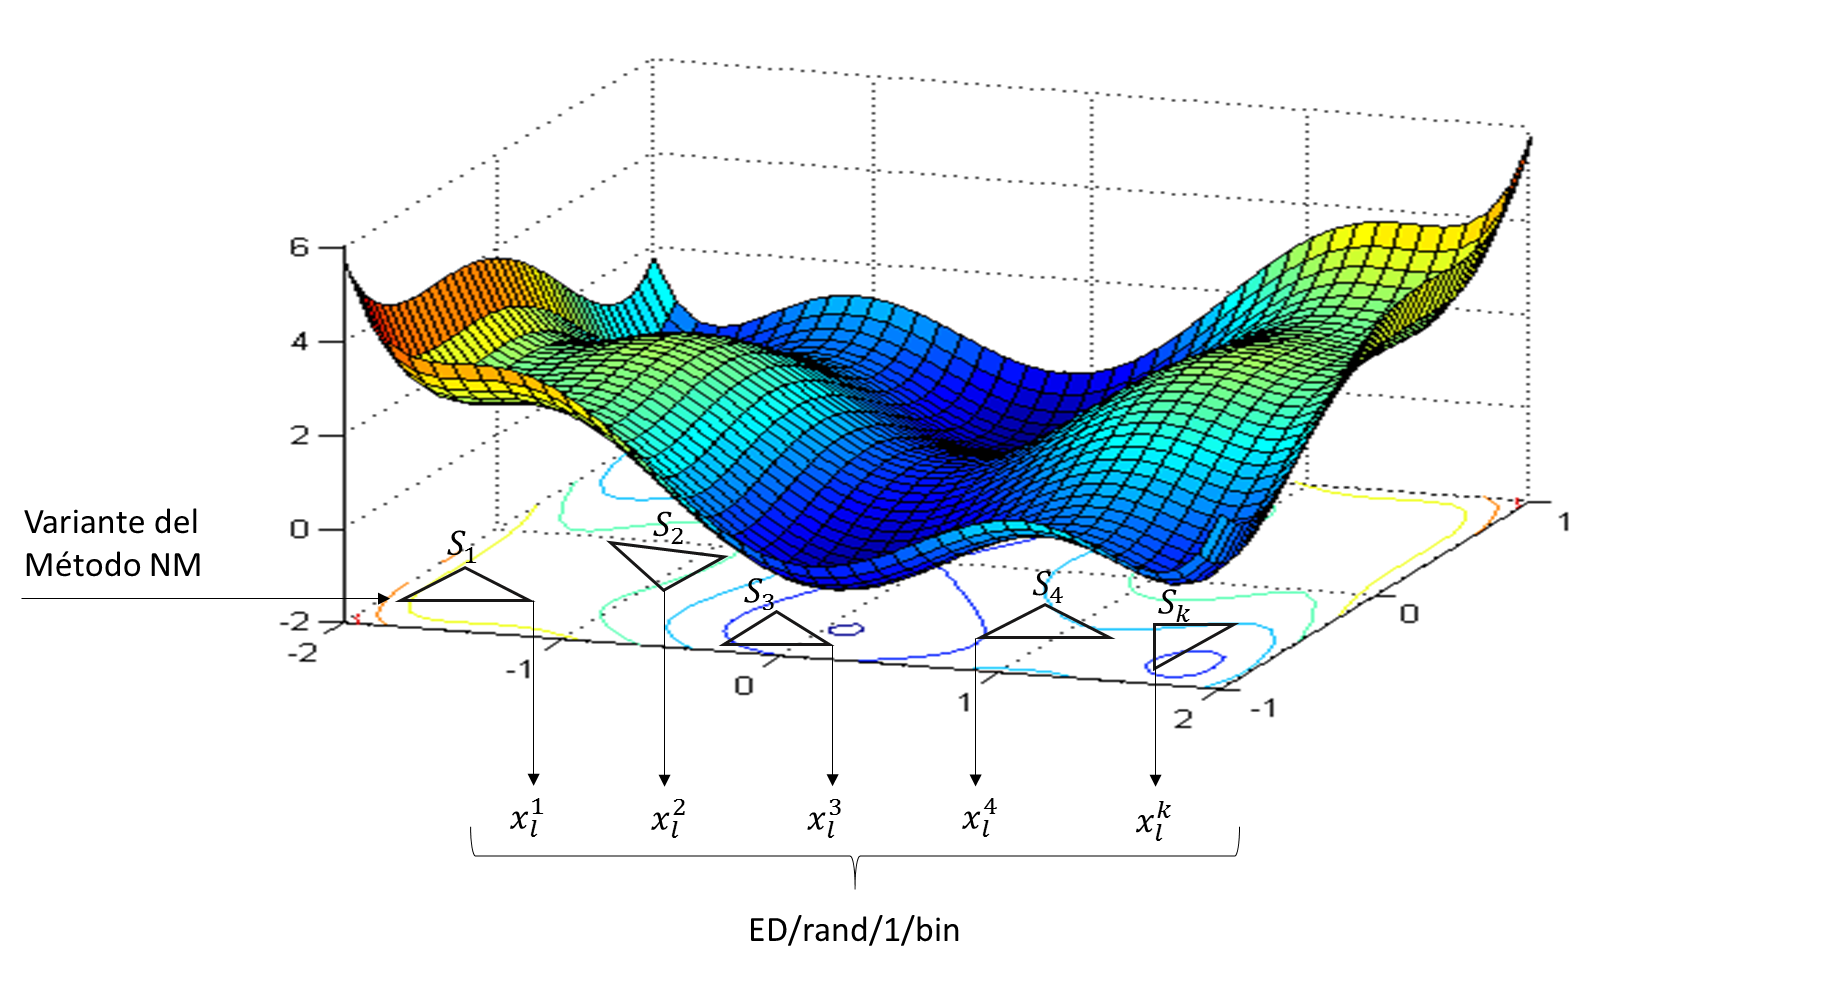
\includegraphics[width=\textwidth]{Figures/Esquema}
		\caption{Esquema de las variantes HNMED.}
		\label{fig:HNMED}
	\end{center}
	\end{figure}


El Algoritmo \ref{alg:HNMED} describe el pseudocódigo para las variantes HNMED. Las flechas rojas en las lineas desde la 26 a la 28 indican el fragmento de código que varía en cada una de las versiones. Donde $NE$ es el número máximo de evaluaciones, $NP$ es el tamaño de la población e $I_{x_l^k}$ el índice correspondiente al punto $x_l^k$ de $S_k$ en la población $X$. En las siguientes secciones se presentan cuatro variantes híbridas bajo el mismo enfoque, las cuales sólo difieren en el operador con aleatoriedad que incluye el método NM. Por tanto, solo se describirán dichos operadores; para mayor detalle sobre la implementación de estas variantes consultar el Anexo \ref{AppendixA}. 


\begin{algorithm}
	\begin{algorithmic}[1]
		\STATE Elegir parámetros: $\beta>0, \gamma \in (0,1)$
		\STATE Generar y evaluar una población aleatoria $X$ inicial.
        \STATE Hacer $E=NP$.
		\WHILE {$E<NE$}
           \STATE Generar $F=(0.3,0.9)$ y $CR=(0,0.8)$
           \FOR{$k \in \{1,\dots,NS\}$}
              \STATE Seleccionar $S_k$ de $X$
              \STATE Ordenar los puntos en $S_k$ de acuerdo a las reglas de Deb.
              \STATE Elegir $x^k_h$, $x^k_l$ y $x^k_g$.
              \STATE Calcular $x^k_c=\frac{1}{N} \sum_{i=1, i\neq h }^{N+1} x^k_i$
              \STATE Realizar la reflexión $x^k_r=2x^k_c -x^k_h$
              \STATE Acotar  $x^k_r$ y evaluar  $f(x^k_r)$
              \IF{$es\_mejor(x^k_r,x^k_l)$}
              \STATE Hacer $x_{new}=(1+\gamma)x^k_c-\gamma x^k_h$ (Expansión)
              \ELSE \IF {$es\_mejor(x^k_h,x^k_r)$}
              \STATE Hacer $x^k_{new}=(1-\beta)x^k_c+\beta x^k_h$ (Contracción adentro)
              \ENDIF
              \ELSE \IF {$es\_mejor(x^k_r,x^k_g) \quad \AND \quad es\_mejor(x^k_h,x^k_r)$}
              \STATE Hacer $x_{new}=(1+\beta)x^k_c-\beta x^k_h$ (Contracción afuera)
              \ENDIF
              \ENDIF
              \STATE Acotar $x^k_{new}$ y evaluar $f(x^k_{new})$
            
              \IF {$es\_mejor(x_h,x_{new})$}

              \STATE $\color{red} \Rightarrow $  Calcular $x^k_{new}$ según la variante  
              \STATE $\color{red} \Rightarrow $ Acotar  $x^k_{new}$ y evaluar  $f(x^k_{new})$  
              \STATE $\color{red} \Rightarrow $ Hacer  $E=E+1$ 
              \ENDIF
              \STATE Seleccionar aleatoriamente índices $r_1 \neq r_2 \neq r_3 \neq I_{x^k_l} $
              \STATE Generar aleatoriamente el índice $randb(j)=(1,N)$ 
              \FOR{$j \in \{1,\dots,N\}$}
                \IF{($randb(j) \leq CR) \quad \OR \quad (j==randb(j))$}
              	   \STATE $u^k_{j} = x_{r_1} + F (x_{r_2}-x_{r_3})$
              	\ELSE 
                  \STATE $u^k_{j} = x^k_{l_j}$
                \ENDIF
              \ENDFOR
             \STATE Acotar $u^k$ y evaluar $f(u^k)$
               \IF{ es\_mejor($f(u^k),x^k_l)$}
                  \STATE $x^k_l = u^k$
               \ENDIF
                 \STATE Hacer  $E=E+3$
        \ENDFOR
		\ENDWHILE
	\end{algorithmic}
	\caption{Algoritmo HNMED}\label{alg:HNMED}
\end{algorithm}

\subsubsection{HNMED. Variantes II y III}
La segunda variante difiere en la versión del NM utilizada. Si los operadores del Nelder Mead no mejoran al peor vector este se sustituye por un vector que tiene como base el mejor vector local $x^k_l$ y va hacia la dirección del mejor individuo en la población $best$ según describe la Ecuación \ref{eq:HNMED2-1}.
\begin{center}
\begin{equation}\label{eq:HNMED2-1}
x_{new}= x^k_l+ F(best-x^k_h)
\end{equation}
\end{center}
Este operador está basado en el cálculo del vector ruido de la mutación diferencial, nótese que $F$ es el mismo factor de escala utilizado en la mutación de la ED. En este caso, las instancias del Nelder Mead tienen un operador que utiliza información global: el mejor individuo en la población. El objetivo aquí es acercar el peor punto en el simplex $S_k$ al mejor punto a nivel global de forma paulatina.

La tercera variante procede de la siguiente forma: en dependencia de cual dirección sea mejor, el vector ruido se dirigirá hacia el mejor punto a nivel global (Ecuación \ref{eq:HNMED2-1}) o se alejará del peor a nivel local con un tamaño de paso proporcional a la diferencia absoluta entre $best$ y $x^k_h$. Esta versión contiene el operador de la Variante II y agrega  un segundo operador (Ecuación \ref{eq:HNMED3-1}) que calcula un vector que tiene como base al mejor individuo local $x^k_l$ y que va en sentido contrario al peor vector local $x^k_h$.
\begin{center}
\begin{equation}\label{eq:HNMED3-1}
x_{new}= x^k_l- F(x^k_h-best)
\end{equation}
\end{center}
De forma similar a la estrategia seguida en NM2ELA el objetivo de utilizar dos operadores que presentan direcciones opuestas es aumentar la capacidad de exploración del buscador local y aumentar la diversidad en simplex para evitar convergencia prematura o estancamiento de las diferentes instancias.
\subsubsection{HNMED. Variantes IV y V }
Las últimas dos variantes están basadas en los operadores utilizados por la versión DE/current-to-best/1 para calcular el vector ruido. El propósito de estas variantes es evitar las dos evaluaciones de la variante III, incorporando más información global en el operador. Los vectores $x_{r_1}$,$x_{r_2}$ y $x_{r_3}$ son seleccionado aleatoriamente de toda la población y cumplen la condición de $ I_{x^k_l} \neq r_1 \neq r_2 \neq r_3$. Nótese que en el tercer miembro de la Ecuación \ref{eq:HNMED4-1} el factor de escala es $1-F$ el cual es el complemento de la probabilidad de $F$. Esta modificación se aplica con el objetivo de mantener un balance entre el miembro elitista y el aleatorio en el operador.
\begin{center}
\begin{equation}\label{eq:HNMED4-1}
%xl(1:n)+F*(best(1:n)-r1(1:n))+(1-F)*(r2(1:n)-r3(1:n))
x_{new}= x^k_l+F(best-x_{r_1})+(1-F)(x_{r_2}-x_{r_3})
\end{equation}
\end{center}
Los operadores propuestos hasta el momento utilizan como vector base un punto local ($x^k_l$). En la quinta variante, el operador utiliza como vector base uno de los vectores elegidos aleatoriamente, una vez más en la búsqueda de aumentar la exploración del espacio de búsqueda y mantener la diversidad de la población. El operador utilizado en la variante V se describe en la ecuación \ref{eq:HNMED5-1}
\begin{center}
\begin{equation}\label{eq:HNMED5-1}
%xl(1:n)+F*(best(1:n)-r1(1:n))+(1-F)*(r2(1:n)-r3(1:n))
x_{new}= x_{r_1}+F(best-x_{r_1})+(1-F)(x_{r_2}-x_{r_3})
\end{equation}
\end{center}
 %xnew1=r1(1:n)+F*(best(1:n)-r1(1:n))+(1-F)*(r2(1:n)-r3(1:n));
Diferentes variantes y combinaciones de estos operadores fueron implementadas. No obstante, se presentan las propuestas que mostraron un mejor rendimiento promedio para los problemas a resolver en la presente investigación. 
\\
\subsubsection{HNMED. Variante VI}
En el diseño inicial de las variantes HNMED se concibió la inicialización de la población de forma aleatoria de acuerdo al procedimiento del enfoque evolutivo. Sin embargo, se pasa por alto la naturaleza geométrica de los operadores utilizados por el Nelder Mead. En \cite{spendley_sequential_1962}, Spendley plantea que un simplex inicial regular puede aumentar el desempeño de un método basado en simplex y plantea las fórmulas para generar un simplex regular de longitud $d$ tomando como centro del simplex un punto $c$ determinado. Por otra parte, Han y Neumann en \cite{han_effect_2006} comprueban que la tasa de convergencia $\rho$ del NM tiende a 1 a medida que aumenta respecto al número de variables $n$, esto es $ \lim_{n\to\infty}\rho(S_0,n)=1$. Incluso, los resultados experimentales muestran que para $\rho(S_0,32)=0.9912$, lo que indica que este efecto sucede rápidamente. Además, algunas consideraciones sobre el comportamiento del método NM original son presentadas: las operaciones de expansión y contracción producen una mayor reducción de la función que las operaciones de reflexión, y un simplex inicial de bordes más largos contribuye a una mejor minimización de la función objetivo. 

Teniendo en cuenta lo planteado en los párrafos anteriores y los resultados obtenidos durante la experimentación con las primeras variantes, se diseña un última versión (Véase Algoritmo \ref{alg:HNMEDV6}) que tiene como objetivo alcanzar una mayor capacidad de exploración en problemas de mayor dimensión. Dos modificaciones principales son llevadas a cabo respecto a las versiones anteriores:
\begin{enumerate}
	\item Se reemplaza la inicialización aleatoria de la población por el siguiente procedimiento: cada punto $x_i$ con $i =\left\lbrace  1,2,...,N+1\right\rbrace $ en  el simplex $S_k$ se genera de acuerdo a la siguiente formula:
	\begin{equation}\label{eq:Inicializacion de Simpleces}
	x^i_j=\begin{cases}
	\frac{u_j-l_j}{2}+p_j(\frac{u_j-l_j}{2}), & \text{si $i==j$}.\\
	u_j+q_k(\frac{u_j-l_j}{2})+r_j, & \text{en caso contrario}.
	\end{cases}
	\end{equation}
	Donde $u_j$ y $l_j$ son los limites superior e inferior en la dimensión $j$. Los valores de  $p_j$, $q_k$ y $r_j$ son números aleatorios de una distribución uniforme en los intervalos siguientes:
	\begin{equation}
	p_j \in \begin{cases}
	(0.05;5n/100), & \text{si $5n/100 <0.95$}.\\
	(0.05;0.95), & \text{en caso contrario}.
	\end{cases}
	\end{equation}
	
	\begin{equation}
	q_k \in \begin{cases}
	(0.5;3n/100), & \text{si $3n/100 <0.95$}.\\
	(0.05;0.95), & \text{en caso contrario}.
	\end{cases}
	\end{equation}
	\begin{equation}
	r_j \in (-NP/100,+NP/100) 
	\end{equation}
	La Ecuación \ref{eq:Inicializacion de Simpleces} esta basada en la presentada por Spendley en \cite{spendley_sequential_1962} para la generación de un simplex regular de longitud $d$, la cual fue concebida para un algoritmo que utiliza un solo simplex y no contempla la diversidad en las dimensiones requerida por la parte evolutiva para un desempeño correcto. Aquí se garantiza una distancia mínima entre los vértices del simplex los cuales se ubicarán en vecindades cercanas a los límites del espacio de búsqueda. Por ejemplo, el punto $x_1$ del simplex $S_k$  estará desplazado en su primera componente hacia región de longitud $(\frac{5n}{100}-0.05)\frac{u_1-l_1}{2}$ en la vecindad del límite superior de la primera dimensión. El punto $x_2$ desplazado hacia el límite superior de la segunda dimensión y así sucesivamente. Finalmente, el punto $x_{n+1}$ se ubicará en la vecindad $(\frac{3n}{100}-0.05)\frac{u_j-l_j}{2}$ de los límites inferiores en todas las dimensiones. El valor aleatorio $r_j$ se utiliza para garantizar una variación de los valores en la dimensión $j$ para el simplex $S_k$. El objetivo de esta inicialización de los símpleces es garantizar tetraedros más regulares y de mayor tamaño. 
	
	\item Las versiones iniciales de HNMED tenían un enfoque elitista. En el caso de HNMED-V4 y HNMED-V5 se utiliza la dirección del mejor para mejorar el peor punto de simplex y la ED sólo se aplicaba al los mejores puntos de cada simplex. Para garantizar que mayor cantidad de individuos reciban información global, los operadores son aplicados a una posición del simplex en cada generación ascendentemente. Esto es, que para la generación 1 la ED se aplica al individuo en la posición 1 en cada simplex, en la segunda generación al individuo en la posición 2 y así sucesivamente hasta llegar a la posición $NS+1$ donde se comienza de nuevo por la primera posición.  
	\item El operador de mutación diferencial utilizado es basado en DE/current-to-best/1:
	\begin{equation}
	v_m= x_m+F(x^r_l-x_{r_1})+(1-F)(x_{r_2}-x_{r_3})
	\end{equation}
	Donde el individuo elitista $x^r_l$ es seleccionado aleatoriamente del conjunto de los mejores individuos de cada simplex $X_l$. 
\end{enumerate}

\section{Conclusiones del capítulo}
En el presente capítulo se propone un nuevo enfoque de hibridación que tiene como objetivo aumentar la eficiencia de la búsqueda usando como base un buscador local. Mediante la distribución de varias instancias en el espacio de búsqueda, el buscador local se potencia  con la capacidad de exploración. El buscador global se utiliza como mecanismo de coordinación entre las diferentes instancias del método de búsqueda local. El número de evaluaciones destinadas al buscador local y global no debe ser desproporcionada para garantizar un balance entre la explotación y la exploración. Además, se plantea la idea de que, aunque cada buscador podrá informarse del resto de la población, sólo se aplicarán a un subconjunto de ella por generación, lo que implica una reducción considerable del número de evaluaciones.

Bajo las directrices de este enfoque se diseñaron e implementaron seis variantes híbridas. Se utilizó como buscador local variantes del método Nelder Mead con operadores que incluyen aleatoriedad e información global. El método NM fue seleccionado por sus características en cuanto a número de evaluaciones, complejidad temporal y los resultados alcanzados en el diseño experimental de las versiones con Expansión de Longitud Aleatoria. La ED/rand/1/bin se selecciona por utilizar vectores seleccionados aleatoriamente de toda la población para la creación del vector ruido por lo que su búsqueda brinda mayor información global. El número de evaluaciones por iteración en comparación con la ED, se reduce a medida que aumenta la dimensionalidad del problema en proporción de $\frac{4}{N+1}$.

Una última versión es diseñada de acuerdo a los resultados del diseño experimental. En la versión seis, se tiene en cuenta la naturaleza geométrica del método Nelder Mead. La generación inicial de los símpleces de forma aleatoria, implicaba la irregularidad y el traslape de estos. Para controlar esta deficiencia se aplica una estrategia de inicialización de los símpleces que garantiza figuras de mayor tamaño y regularidad.  

\begin{algorithm}
	\begin{algorithmic}[1]
		\STATE Elegir parámetros: $\beta>0, \gamma \in (0,1)$
		\STATE $\color{red} \Rightarrow $ Generar símpleces según Equación \ref{eq:Inicializacion de Simpleces} y evaluar $X$.
		\STATE Hacer $E=NP$.
		\WHILE {$E<NE$}
		\STATE Generar $F=(0.3,0.9)$ y $CR=(0,0.8)$
		\FOR{$k \in \{1,\dots,NS\}$}
		\STATE Seleccionar $S_k$ de $X$
		\STATE Ordenar los puntos en $S_k$ de acuerdo a las reglas de Deb.
		\STATE Elegir $x^k_h$, $x^k_l$ y $x^k_g$.
		\STATE Calcular $x^k_c=\frac{1}{N} \sum_{i=1, i\neq h }^{N+1} x^k_i$
		\STATE Realizar la reflexión $x^k_r=2x^k_c -x^k_h$
		\STATE Acotar  $x^k_r$ y evaluar  $f(x^k_r)$
		\IF{$es\_mejor(x^k_r,x^k_l)$}
		\STATE Hacer $x_{new}=(1+\gamma)x^k_c-\gamma x^k_h$ (Expansión)
		\ELSE \IF {$es\_mejor(x^k_h,x^k_r)$}
		\STATE Hacer $x^k_{new}=(1-\beta)x^k_c+\beta x^k_h$ (Contracción adentro)
		\ENDIF
		\ELSE \IF {$es\_mejor(x^k_r,x^k_g) \quad \AND \quad es\_mejor(x^k_h,x^k_r)$}
		\STATE Hacer $x_{new}=(1+\beta)x^k_c-\beta x^k_h$ (Contracción afuera)
		\ENDIF
		\ENDIF
		\STATE Acotar $x^k_{new}$ y evaluar $f(x^k_{new})$
		
		\IF {$es\_mejor(x_h,x_{new})$}
		
		\STATE $\color{red} \Rightarrow $  Calcular  $x_{new}= x_{r_1}+F(best-x_{r_1})+(1-F)(x_{r_2}-x_{r_3})$
		\STATE Acotar  $x^k_{new}$ y evaluar  $f(x^k_{new})$  
		\STATE Hacer  $E=E+1$ 
		\ENDIF
		\STATE $\color{red} \Rightarrow $ Seleccionar aleatoriamente índices $r=$(1,N+1) y $r_1 \neq r_2 \neq r_3 \neq I_{x^k_l} $
		\STATE Generar aleatoriamente el índice $randb(j)=(1,N)$ 
		\FOR{$j \in \{1,\dots,N\}$}
		\IF{($randb(j) \leq CR) \quad \OR \quad (j==randb(j))$}
		\STATE $\color{red} \Rightarrow $ $u^k_{j} =  x^k_{mj}+F(x^r_l-x_{r_1})+(1-F)(x_{r_2}-x_{r_3})$
		\ELSE 
		\STATE $\color{red} \Rightarrow $ $u^k_{j} = x^k_{mj}$
		\ENDIF
		\ENDFOR
		\STATE Acotar $u^k$ y evaluar $f(u^k)$
		\IF{ es\_mejor($f(u^k),x^k_l)$}
		\STATE $\color{red} \Rightarrow $ $x^k_m = u^k$
		\ENDIF
		\STATE Hacer  $E=E+3$
		\ENDFOR
		\STATE $\color{red} \Rightarrow $ Hacer  $m=m+1$
		\ENDWHILE
	\end{algorithmic}
	\caption{HNMED. Variante IV}\label{alg:HNMEDV6}
\end{algorithm} 
\chapter{Experimentos y Resultados} \label{Chapter7}

La investigación de algoritmos metaheurísticos y, especialmente, en la computación evolutiva (CE) se basa principalmente en dos pilares: la teoría y la práctica. Sin embargo, la mayor parte del trabajo publicado en esta área se dedica a la aplicación de la CE y los métodos relacionados a problemas reales o de referencia. En la teoría de análisis de algoritmos la medición del desempeño de un método determinado se enfoca fundamentalmente el conocer cómo este funciona para el peor caso posible. Por otra parte, las investigaciones experimentales rara vez se preocupan por los peores casos, sobre todo si el problema tiene un trasfondo del mundo real, donde la observación del peor caso puede ser poco probable. Por lo tanto, el mayor interés se centra en el promedio de cierta cantidad los casos. Los trabajos experimentales han tenido dos motivaciones principales: resolver problemas del mundo real o al menos demostrar que pueden ser resueltos mediante un algoritmo evolutivo y demostrar la eficacia de un algoritmo (preferiblemente nuevo) en una clase de problemas. La realización de experimentos en ciencias de la computación puede requerir las siguientes tareas \cite{BartzBeielstein2014ExperimentalAO}:
\begin{enumerate}
	\item Encontrar los mejores parámetros o algoritmos dados $k$ conjuntos de números aleatorios representando el resultado de ciertos experimentos.
	\item  Encontrar la mejor asignación para un conjunto de variables reales (dentro de un rango dado) que representan los parámetros del algoritmo para una clase de problema.
	\item Dadas las posibles formas de modificar un algoritmo $A$ (por ejemplo, mediante el uso de operadores adicionales) encontrar la mejor combinación para una clase de problema.
\end{enumerate}
El presente capítulo se enfoca fundamentalmente en esta última tarea. Sin embargo, las muestras que se pueden obtener para realizar las comparaciones en número determinado de aspectos como: operadores, problemas de optimización, parámetros, número de evaluaciones entre otros; no permiten necesariamente obtener conclusiones generales sobre los algoritmos comparados. Por tanto, la pregunta de investigación más adecuada es bajo qué condiciones  un algoritmo $A$ es mejor que $A'$ y por qué. En este caso, se trata de comparar los algoritmos propuestos con aquellos algoritmos que mejores resultados han obtenido en el conjunto específico de problemas planteados. 
\section{Diseño Experimental}

El diseño experimental de la propuesta de solución se estructuran de acuerdo a la metodología planteada a continuación. El objetivo  de especificar una metodología es organizar el proceso de experimentación y garantizar la calidad de los resultados. Se plantea una metodología que contempla los siguientes pasos basados en \cite{BartzBeielstein2014ExperimentalAO}:
\begin{enumerate}
	\item\textbf{ Planteamiento objetivos del experimento}: para cada tipo experimento se debe indicar si se realizan para:
	\begin{enumerate}
		\item Demostrar el rendimiento de un algoritmo.
		\item Verificar la robustez de un algoritmo en varias instancias de problema.
		\item Comparar dos (o varios) algoritmos conocidos.
		\item Explicar o comprender un comportamiento observado y detectar novedades. 
	\end{enumerate}
	\item \textbf{Definición de medidas y pruebas de desempeño}: Con base en los objetivos del experimento se debe definir cómo realizar las mediciones:
	\begin{enumerate}
		\item El rendimiento será medido en términos del número de evaluaciones de la función objetivo.
		\item Para medir la robustez del algoritmo se utilizará la estadística descriptiva: medidas de tendencia central y de dispersión de una muestra de $n$ ejecuciones del algoritmo $A$.
		\item La comparación de los algoritmos se realizará mediante pruebas de estadística inferencial: Pruebas de Friedman, Bonferroni-Dunn, prueba no paramétrica de suma de rangos de Wilcoxon.
		\item Se utilizarán medidas como tasa de éxito de los operadores, medidas de diversidad y gráficas de convergencia para explicar o comprender comportamientos y detectar novedades.
	\end{enumerate}
	\item \textbf{Planificación pre-experimental y configuración}: Este paso abarca la selección del número máximo permitido de evaluaciones de la función objetivo, el conjunto de problemas a resolver, número de ejecuciones para obtener las muestras y número de comparaciones a realizar. Se debe implementar y describir todo lo necesario para replicar el experimento. Esto consiste en la implementación y documentación de los algoritmos, problemas, parámetros y condiciones externas importantes como detalles del hardware empleado.
	\item \textbf{Realización de los experimentos}: Los experimentos deberán ser realizados de forma automática. Las implementaciones deberán estar debidamente comentadas y los resultados deben ser presentados de forma organizada.
	
	\item \textbf{Resultados y Visualización }: Se resumen y presentan los resultados numéricos, pruebas de hipótesis, así como las tablas o figuras obtenidas a partir de los experimentos.
	\item \textbf{Observaciones}: Reportar el comportamiento inesperado o notable detectado mediante la revisión de los resultados, sin interpretación. Se debe discutir la relevancia estadística. Si las hipótesis estadísticas son aceptadas o rechazadas. Discutir el significado científico de lo observado: explicaciones de los resultados del experimento en contexto con otros hallazgos científicos. Este paso está destinado a contener declaraciones subjetivas que pueden conducir a nuevas hipótesis o preguntas de investigación basadas en los resultados de los experimentos actuales.
\end{enumerate}

\section{Estadística inferencial: Pruebas estadísticas no paramétricas}
Para la realización de las comparaciones entre los algoritmos propuestos y los de mejor desempeño encontrados en la literatura se utilizarán medidas de estadística  descriptiva y pruebas de estadística no paramétrica. A diferencia de la estadística descriptiva, cuyos cálculos son sencillos y de conocimiento general; las pruebas de estadística no paramétrica presentan procedimientos más complejos y se debe explicar claramente para que se utiliza cada una de estas pruebas.

La tarea esencial de la estadística inferencial es determinar conclusiones sobre un dominio completo de fenómenos (una población), a partir del análisis de una muestra limitada de instancias extraídas de ese dominio. Para lograr esto, se formulan dos hipótesis sobre el fenómeno. La hipótesis nula $H_0$ enuncia que no existen diferencias entre los fenómenos observados y la hipótesis alternativa $H_1$  el caso contrario. Sin embargo, la visión del fenómeno proporcionada por la muestra puede representar o no la realidad objetiva; esta última posibilidad se deriva del hecho de que los fenómenos en naturaleza pueden presentar variabilidad aleatoria. En cualquier caso, hasta que se evalúe rigurosamente esa posibilidad, no se pueden extraer conclusiones razonables de una muestra. La significación estadística es el aparato lógico y matemático mediante el cual se lleva a cabo esa evaluación. \cite{Lowry2004}.

En las pruebas no paramétricas, el estadístico $p$ es calculado en lugar de definir un valor de significancia a priori. El valor de $p$ determina el nivel de significancia resultante de rechazar $H_0$ y provee información sobre si la prueba estadística es significativa o no. A menor valor de $p$, resulta mayor la evidencia en contra de $H_0$. Luego el rechazo o aceptación de cada hipótesis se realiza de la siguiente forma:
\begin{eqnarray}
\text{Si } p \leq \alpha,& \text{se acepta } H_1.\\
\text{Si } p> \alpha,& \text{se acepta } H_0.
\end{eqnarray}

Donde $\alpha$ es un valor que determina el nivel de significancia mínimo necesario para aceptar $H_0$. Las pruebas no paramétricas en su concepto inicial se ejecutan sobre datos nominales. Sin embargo, pueden ser aplicadas a datos continuos mediante la jerarquización de los datos de entrada. Existen dos clases de análisis: comparaciones por pares y comparaciones múltiples. Los procedimientos estadísticos por pares realizan comparaciones individuales entre dos muestras, obteniendo en cada aplicación un valor $p$ independiente de otro. Por lo tanto, para llevar a cabo una comparación que involucre más de dos muestras, se deben usar pruebas de comparaciones múltiples. Ambas clases de análisis pueden ser utilizados para comparar el desempeño de dos algoritmos, siendo las observaciones en las muestras el resultado de las ejecuciones de los métodos y  la población el desempeño general (número infinito de ejecuciones ) del algoritmo en un problema determinado.  Entonces, la hipótesis $H_0$ plantea que no existen diferencias significativas en el desempeño general de dos algoritmos y $H_1$ afirma lo contrario   \cite{derrac2011practical}.


\subsection{Prueba de suma de jerarquías de Wilcoxon}

La prueba de la suma de jerarquías de Wilcoxon es una prueba no paramétrica que utiliza  datos muestrales jerarquizados de dos poblaciones independientes. La prueba de suma de jerarquías de Wilcoxon a menudo se describe como la versión no paramétrica de la prueba $t$ de dos muestras. A diferencia de la prueba $t$, que asume la distribución normal de las poblaciones, aquí no se asume que existe una distribución conocida. La tasa de eficiencia de prueba de esta prueba es de 0.95 en comparación con la prueba paramétrica $t$. La hipótesis nula $H_0$ plantea que las muestras independientes provienen de poblaciones con medianas iguales. La hipótesis alternativa $H_1$ es la aseveración de que las dos poblaciones tienen medianas diferentes. Dadas dos muestras $M_1$ y $M_2$ de tamaño $n_1$ y $n_2$ respectivamente, el procedimiento a seguir el siguiente:
\begin{enumerate}
	\item Combinar temporalmente las dos muestras  en una muestra de tamaño $M'$.
	\item Reemplazar cada valor muestral por su jerarquía. Esto es, remplazar el mejor valor por 1 y el peor por 2 para cada par de valores en la muestra. En caso de empate asignar el promedio de las jerarquías a ambos elementos.
	\item Separar las muestras y calcular la suma de los rangos $R_1$ y $R_2$ de las dos muestras.
	\item Calcular el valor del estadígrafo de prueba:
	\begin{eqnarray}
	&& z= \frac{R-\mu_R}{\sigma_R}
	\end{eqnarray}
	Donde:
	\begin{eqnarray}
	&& \mu_R=\frac{n_1(n_1+n_2+1)}{2}\\
	&& \sigma_R= \sqrt{\frac{n_1n_2(n_1+n_2+1)}{12}}
	\end{eqnarray}
	El valor de $R$ corresponde a la suma de rangos obtenida en la muestra $M$. Cualquiera de las dos muestras se puede utilizar para calcular el estadígrafo. 
	\item La prueba de hipótesis se realiza con un nivel de significancia $\alpha=0.05$ que corresponde a un valor crítico de $\pm 1.96$. Luego:
	\begin{eqnarray}
	\text{Si } z > 1.96 \text{  o'  } z < -1.96,& \text{se acepta } H_1\\
	\text{En caso contrario}  ,& \text{se acepta } H_0
	\end{eqnarray}
\end{enumerate}



\subsection{Pruebas de Friedman}
La prueba de Friedman es una prueba de comparaciones múltiples que puede ser utilizada para detectar diferencias significativas entre el comportamiento de dos o más algoritmos. De forma general, la prueba de Friedman dictamina si para un conjunto de $k \geq 2$ muestras, al menos dos de estas representan poblaciones con medianas diferentes. Estas pruebas son análogas a las pruebas ANOVA de medidas repetidas en procedimientos estadísticos no paramétricos. 

De forma similar a otras pruebas de estadística inferencial la hipótesis nula $H_0$ para la prueba de Friedman plantea la igualdad entre las medias de las poblaciones representadas por las muestras y la hipótesis alternativa $H_1$ la negación de $H_0$. El procedimiento general para llevar a cabo esta prueba es el siguiente:
\begin{enumerate}
	\item Conformar una matriz de $k$ columnas (muestras) y $n$ filas (tamaño de las muestras).
	\item Para cada la fila $i$ de la muestra asignar las jerarquías correspondientes (el mejor resultado de la fila toma jerarquía 1, el segundo mejor 2 y así sucesivamente). En caso de empates asignar el promedio de las jerarquías a cada elemento.
	\item Calcular por cada la columna los promedios de jerarquías  $R_j=\frac{1}{n}\sum_i{r_i}$ 
	\item Calcular es estadígrafo:
	\begin{equation}
	F_f=\frac{12n}{k(k+1)}\left [  \sum_j{R_j}-\frac{k(k+1)^2}{4}\right]
	\end{equation}
	Donde $F_f$ se distribuye de acuerdo a $\chi^2$ con el que obtiene el valor de $p$
	\item Realizar la prueba de hipótesis con $\alpha=0.05$:
	\begin{eqnarray}
	\text{Si } p \leq \alpha,& \text{se acepta } H_1.\\
	\text{Si } p> \alpha,& \text{se acepta } H_0.
	\end{eqnarray}
	
\end{enumerate}

\subsection{Pruebas Post-hoc: Bonferroni-Dunn}
El principal inconveniente de las pruebas de Friedman, es que sólo pueden detectar diferencias significativas sobre la comparación múltiple completa, y no pueden establecer comparaciones adecuadas entre algunos de los algoritmos considerados. Cuando el objetivo de la aplicación de las pruebas múltiples es realizar una comparación considerando un método de control y un conjunto de algoritmos, se puede definir una familia de hipótesis, todas relacionadas con el método de control. Entonces, la aplicación de una prueba post-hoc puede conducir a la obtención de un valor p que determina el grado de rechazo de cada hipótesis. Una familia de hipótesis es un conjunto de hipótesis de comparaciones lógicamente interrelacionadas que, en comparaciones $1 x N$, compara los algoritmos $k - 1$ del estudio (excluyendo el control) con el método de control, mientras que en las comparaciones $NxN$ consideran las $\frac{(k-1)}{2}$ posibles comparaciones entre algoritmos. Por lo tanto, la familia de hipótesis estará compuesta de $k - 1$ o $\frac{(k-1)}{2}$ hipótesis, respectivamente, que se pueden ordenar por su valor $\rho$, de menor a mayor.

El valor $\rho$ de cada hipótesis en la familia se puede obtener a través de la conversión de las clasificaciones calculadas por cada prueba usando una aproximación normal. Las pruebas Post hoc se realizan teniendo en cuenta los resultados obtenidos por una prueba de comparación múltiple como la de Friedman. Por tanto, el estadístico de prueba $z$ para comparar el algoritmo i-ésimo y el algoritmo j-ésimo, depende del principal procedimiento no paramétrico utilizado. En caso de realizar una prueba post-hoc a partir de la prueba de Friedman se utilizará el siguiente estadígrafo:
\begin{equation}
z=\frac{R_i-R_j}{\sqrt{\frac{k(k+1)}{6n}}}
\end{equation}

En las pruebas Post Hoc en lugar de calcular un valor de $p$ para probar cada hipótesis, se utilizan valores de $p$ ajustados ($APV$ por sus siglas en inglés). Estos valores tienen en cuenta el error acumulado al realizar múltiples pruebas. Además, los $APV$ se pueden comparar directamente con cualquier nivel de significancia $\alpha$ elegido. Por lo tanto, se recomienda su uso ya que brindan más información en un análisis estadístico. Para la prueba de Bonferroni-Dunn el $APV$ para la hipótesis $i$ se calcula mediante un solo paso multiplicando el número de comparaciones por el valor $p_i$ obtenido.
\begin{equation}
APV_i=min \{v,1\} \text{, donde } v=(k-1)p_i
\end{equation}




%%%%%%%%%%%%%%%%%%%%%%%%%%%%%%%%%%%%%%%%%%%%%%%%%%%%%%%%%%%%%%%%%%%%%%%%%%%%%%%%%%%%
\section{Experimentos preliminares}
Los experimentos preliminares se realizan con el objetivo de implementar las primeras variantes de la propuesta de solución y demostrar la competitividad del enfoque propuesto. Por competitividad del enfoque se entiende que los algoritmos diseñados de acuerdo al enfoque puedan obtener resultados iguales o mejores a los encontrados en la literatura especializada de acuerdo a diferentes pruebas de desempeño. Los resultados obtenidos serán medidos de acuerdo a los siguientes aspectos:
\begin{enumerate}
	\item \textbf{Robustez}: dada por las medidas de tendencia central y de dispersión en una muestra de $n$ ejecuciones. La estadística descriptiva permite conocer si los algoritmos logran encontrar los mínimos conocidos de la función y con qué frecuencia lo hacen. 
	\item \textbf{Eficiencia}: dada por la tasa de convergencia de los algoritmos implementados a partir del enfoque. La taza de convergencia será calculada en función del número de evaluaciones. Permite conocer cuantas evaluaciones necesita un algoritmo determinado para encontrar un valor igual o cercano al mínimo.
	\item \textbf{Nivel de significación}: las pruebas de estadística inferencial se aplicarán para determinar si existen diferencias significativas entre el desempeño (ya sea mejor o peor) de algoritmos propuestos y los encontrados en la literatura especializada.
\end{enumerate}

Para esto se someten a prueba todas las variantes descritas en la sección \ref{sec:HNMEDV1}. Se realizan cuatro experimentos preliminares. El experimento A  consiste en obtener las estadísticas descriptivas para evaluar la robustez del algoritmo y la calidad de las soluciones. Además se realizaran gráficas de convergencia de la ejecución correspondiente a la mediana de la muestra para todos los algoritmos algoritmos propuestos y la  ED/rand/1/bin en los 6 problemas de optimización.

El experimento B consiste en realizar una comparación múltiple entre las variantes propuestas y la ED/rand/1/bin mediante las pruebas de Friedman y Bonferroni-Dunn, manteniendo el mismo número de evaluaciones para los 6 problemas de optimización a resolver. 

En el experimento C se reduce el número de evaluaciones de las variantes híbridas teniendo en cuenta la tasa de convergencia de cada algoritmo. Se realiza un ajuste de parámetros para cada variante y se mide el desempeño tanto desde el punto de vista estadístico  tanto descriptivo como inferencial.

 \subsection{Experimento A: Pruebas de estadísticas sobre el Método Nelder Mead con Expansión de Longitud Aleatoria}\label{Experimento A: Pruebas de estadísticas sobre el Método Nelder Mead con Expansión de Longitud Aleatoria}

 Debido a que la hibridación bajo el enfoque propuesto plantea la interacción entre los métodos de búsqueda local y global, el primer experimento se realiza para responder preguntas de investigación, relacionadas con el comportamiento del Nelder Mead al utilizar aleatoriedad en sus operadores:
 \begin{enumerate}
 	\item ¿ Como introducir aleatoriedad en los operadores del NM para aumentar su capacidad de exploración?
 	\item ¿ Introducir operadores que exploren puntos distantes de la vecindad actual puede aumentar el desempeño en los problemas de optimización a resolver?
 
 \end{enumerate}
Para responder estas interrogantes se plantearon las variantes NMELA descritas en las sección \ref{sec:NMELA}.
 \subsubsection{Definición de medidas}
 Se obtendrá para cada algoritmo una muestra de $n$ ejecuciones. Cada elemento de la muestra es el valor de la función objetivo del mejor individuo factible encontrado en la ejecución $i$ para $i= \{ 1,2,...,n\}$. Para cada muestra se obtendrá:
 \begin{enumerate}
 	\item \textbf{Mejor}: valor mínimo de función objetivo registrado en la muestra.
 	\item \textbf{Peor}: valor máximo registrado en la muestra.
 	\item \textbf{Mediana}: valor que se encuentra en el centro de la muestra ordenada. Esta medida es fundamental para evaluar el desempeño ya que el promedio puede ser afectado por valores anómalos. 
 	\item \textbf{Promedio}: valor característico o tendencia central la muestra.
 	\item \textbf{Desviación estándar}: grado de dispersión de las soluciones registradas en la muestra con respecto al promedio.
 	\item \textbf{Tasa de convergencia}: velocidad con que la mejor solución encontrada se aproxima al mínimo.  
 \end{enumerate}
 \subsubsection{Planificación pre-experimental y configuración}
 Para el presente experimento se generaron 5 muestras por cada problema, correspondientes a los algoritmos NMELA, NMEILA, NM2ELA, las versiones deterministas NM y el método Nelder Mead con operador de encogimiento. Cada muestra tiene un tamaño tamaño $n=31$. Las pruebas se realizaron sobre los resultados obtenidos en los 5 primeros problemas de optimización correspondientes al diseño cinemático. Las ejecuciones se llevaron a cabo en una computadora con procesador AMD Athlon II X2, memoria RAM 2GB, sistema operativo Windows 7 con arquitectura de 64 bits y como entorno de programación se utilizó  MatLab R2016b. 
 
 Para este experimento se utilizó un número fijo de evaluaciones para todos los algoritmos en comparación en cada problema de optimización según se describe en la Tabla \ref{tab:Evaluaciones utilizadas por problema de optimización: Experimento A.}:
 
 \begin{table}[]
 	\centering
 	\caption{Evaluaciones utilizadas por problema de optimización: Experimento A.}
 	\label{tab:Evaluaciones utilizadas por problema de optimización: Experimento A.}
 	\begin{tabular}{cc}
 		\textbf{Problema} &   \textbf{Evaluaciones}     \\
 		\hline
 		MCE1   &   400000       \\
 		MCE2   &   20000       \\
 		MCE3   &   225000      \\
 		GCE1   &   125000       \\
 		GCE2   &   200000      \\
 	\end{tabular}
 \end{table}
 La configuración de parámetros utilizada por las variantes HNMED y la ED es la siguiente:
 \begin{enumerate}
 	\item Para las variantes NMELA se establecieron los parámetros de reflexión $\alpha=2$, expansión $\gamma=1.05$ $\beta=0.5$ para todos los problemas.
 	 	\item Para las variantes determistas se establecieron los parámetros de reflexión $\alpha=2$, expansión $\gamma=1.5$ $\beta=0.5$ para todos los problemas.
 \end{enumerate}
 
 \subsubsection{Presentación de resultados}
 En la Tabla \ref{tab:resultados NMELA} se observan los resultados obtenidos para las medidas de estadística descriptivas definidas para el experimento. Las primeras dos columnas muestran los resultados correspondientes a las variantes deterministas NS(versión descrita en sección \ref{sec: Metodo NM}) y el NM con operador de encogimiento (NMS).  La Figura \ref{fig: Bonferroni-Dunn -NMELA} muestra los resultados de las pruebas post hoc de Bonferroni-Dunn para los 5 problemas de diseño cinemático. Las etiquetas 1 y 2, corresponden al NM y NMS, y las etiquetas 3, 4 y 5 corresponden a NMELA, NMEILA y NM2ELA respectivamente. Las lineas son los intervalos de confianza calculados. En caso de que dos intervalos se traslapen indica que la sub-hipótesis nula se cumple para ambos algoritmos.
 \begin{table}[]  
 	\centering
 	\caption{Resultados estadísticos obtenidos por las versiones aleatorizadas del NM. Los mejores resultados se resaltan en negritas.}
 	\label{tab:resultados NMELA}
 		\resizebox{\textwidth}{!}{%
 	\begin{tabular}{clccccc}
 		\hline
 		Problema              & Estadística   & NM &  NMS     & NMELA               & NMEILA & NM2ELA  \\ 
 		\hline
 		\multirow{6}{*}{MCE1} & Mejor        &6.7163E-06&1.3720E-01 &4.9641E-26&3.1550E-25&\textbf{ 3.0569E-26 } \\
 		& Peor         &4.3821E+02 &4.5506E+02&\textbf{4.3750E+02}&4.3750E+02&9.7062E+03 \\
 		& Mediana      &9.1467E-01 &4.3196E+01&\textbf{2.0672E-02}&9.3146E-04&2.0673E-02 \\
 		& Promedio     &6.6808E+01 &9.6835E+01&7.4217E+01&\textbf{4.5667E+01}& 7.5356E+02 \\
 		& Desv. Est.   &1.4200E+02 &1.4305E+02&1.5845E+01&\textbf{1.1869E+01}&2.1343E+03 \\
 		& Evaluaciones &\multicolumn{5}{c}{\textbf{400000}}\\
 		
 		\hline
 		\multirow{6}{*}{MCE2} & Mejor        &2.6590E-03&7.2367E-04&3.8155E-04&2.6280E-03&\textbf{3.8126E-04} \\
 		& Peor         &7.7302E+03&1.2757E-01&3.9431E+00&\textbf{1.4211E-02}&3.2957E-01  \\
 		& Mediana      &3.6442E-03&3.7092E-03&\textbf{2.6281E-03}&2.6288E-03&\textbf{2.6281E-03 } \\
 		& Promedio     &2.7292E+02&9.5048E-03&1.3391E-01&\textbf{3.0235E-03}&1.3837E-02  \\
 		& Desv. Est.   &1.4109E+03&2.3509E-02&7.1944E-01&\textbf{2.1132E-02}&5.9671E-02  \\
 		& Evaluaciones &\multicolumn{5}{c}{\textbf{20000}}\\
 		
 		\hline
 		\multirow{6}{*}{MCE3} & Mejor        &1.9620E+00&2.9152E+01& 2.7496E-01&\textbf{2.7496E-01}&2.7496E-01 \\
 		& Peor         &2.5350E+03 &4.2133E+04&\textbf{1.3508E+01}&1.4420E+01&1.3508E+01 \\
 		& Mediana      &1.5008E+01&6.3121E+01&4.7321E-01&\textbf{1.1410E+00}&1.2710E+00 \\
 		& Promedio     &4.3987E+02&1.9493E+03&\textbf{4.4381E+00}&5.0760E+00&5.0759E+00 \\
 		& Desv. Est.   &8.3627E+02&7.7310E+03&\textbf{6.0582E+00}&6.2441E+00 &6.0650E+00 \\
 		& Evaluaciones &\multicolumn{5}{c}{\textbf{225000}}\\
 		\hline
 		\multirow{6}{*}{GCE1} & Mejor        &4.4681E-27&9.0876E-28&1.0602E-27&\textbf{3.1554E-30}&8.7090E-28\\
 		& Peor         &3.3175E+05&1.5295E+05&\textbf{1.2863E+05}&3.3973E+05&1.1731E+05 \\
 		& Mediana      &1.4012E+04&1.7275E+02&4.4855E-01&\textbf{5.6447E-15}&5.5696E+02 \\
 		& Promedio     &5.4149E+04&2.5236E+04&\textbf{7.6006E+03}&1.8545E+04&7.7064E+03 \\
 		& Desv. Est.   &8.3973E+04&4.4103E+04&2.4672E+04&6.2803E+04&\textbf{2.3619E+04}\\
 		& Evaluaciones &\multicolumn{5}{c}{\textbf{125000}}\\
 		\hline
 		\multirow{6}{*}{GCE2} & Mejor        &1.1872E-01&1.3937E-01&1.1399E-01 &1.1391E-01&\textbf{1.1389E-01}\\
 		& Peor         &2.8728E+05&2.5495E+05&\textbf{6.8139E+04}&7.2095E+04&1.5666E+05\\
 		& Mediana      &7.6415E+03&1.1269E+02&1.0466E+00&\textbf{1.7267E-01}&5.1727E-01\\
 		& Promedio     &5.3444E+04&1.5327E+04&1.1382E+04&\textbf{4.6427E+03}&1.0443E+04\\
 		& Desv. Est.   &8.3696E+04&5.0724E+04&2.2244E+04&\textbf{1.5319E+04}& 3.3321E+04\\
 		& Evaluaciones &\multicolumn{5}{c}{\textbf{200000}}\\
 		\hline
 	\end{tabular}
}
 \end{table}

\begin{figure}
	\centering
	\begin{subfigure}[b]{0.49\linewidth}
		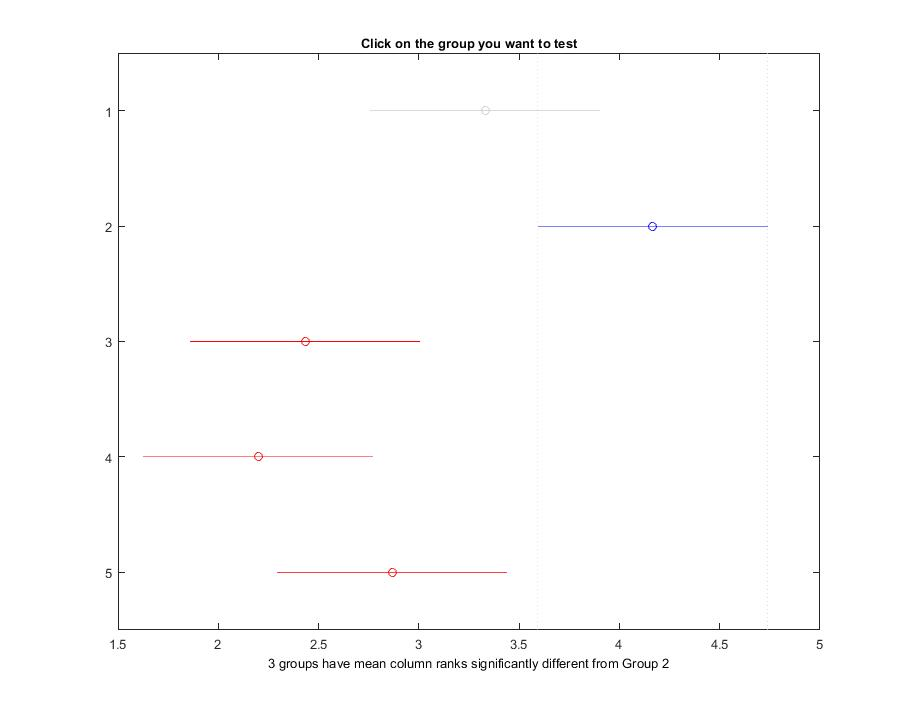
\includegraphics[width=\linewidth]{Figures/NMELA_FB_P1}
		\caption{MCE1} \label{fig:M1} 
	\end{subfigure}
	\begin{subfigure}[b]{0.49\linewidth}
		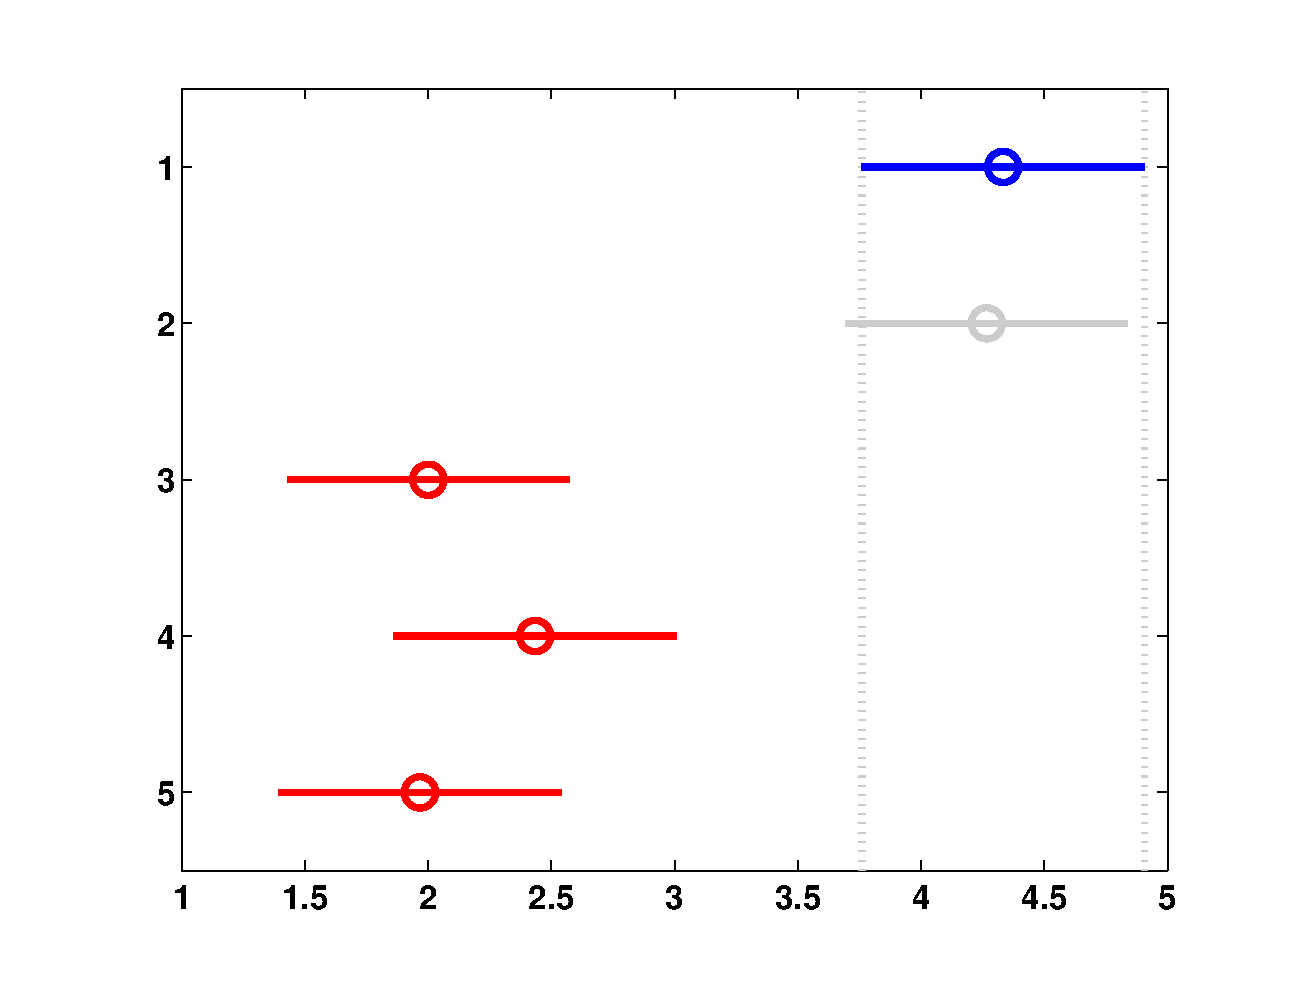
\includegraphics[width=\textwidth]{Figures/NMELA_FB_P2}
		\caption{MCE2} \label{fig:M2} 
	\end{subfigure}
	\begin{subfigure}[b]{0.49\linewidth}
		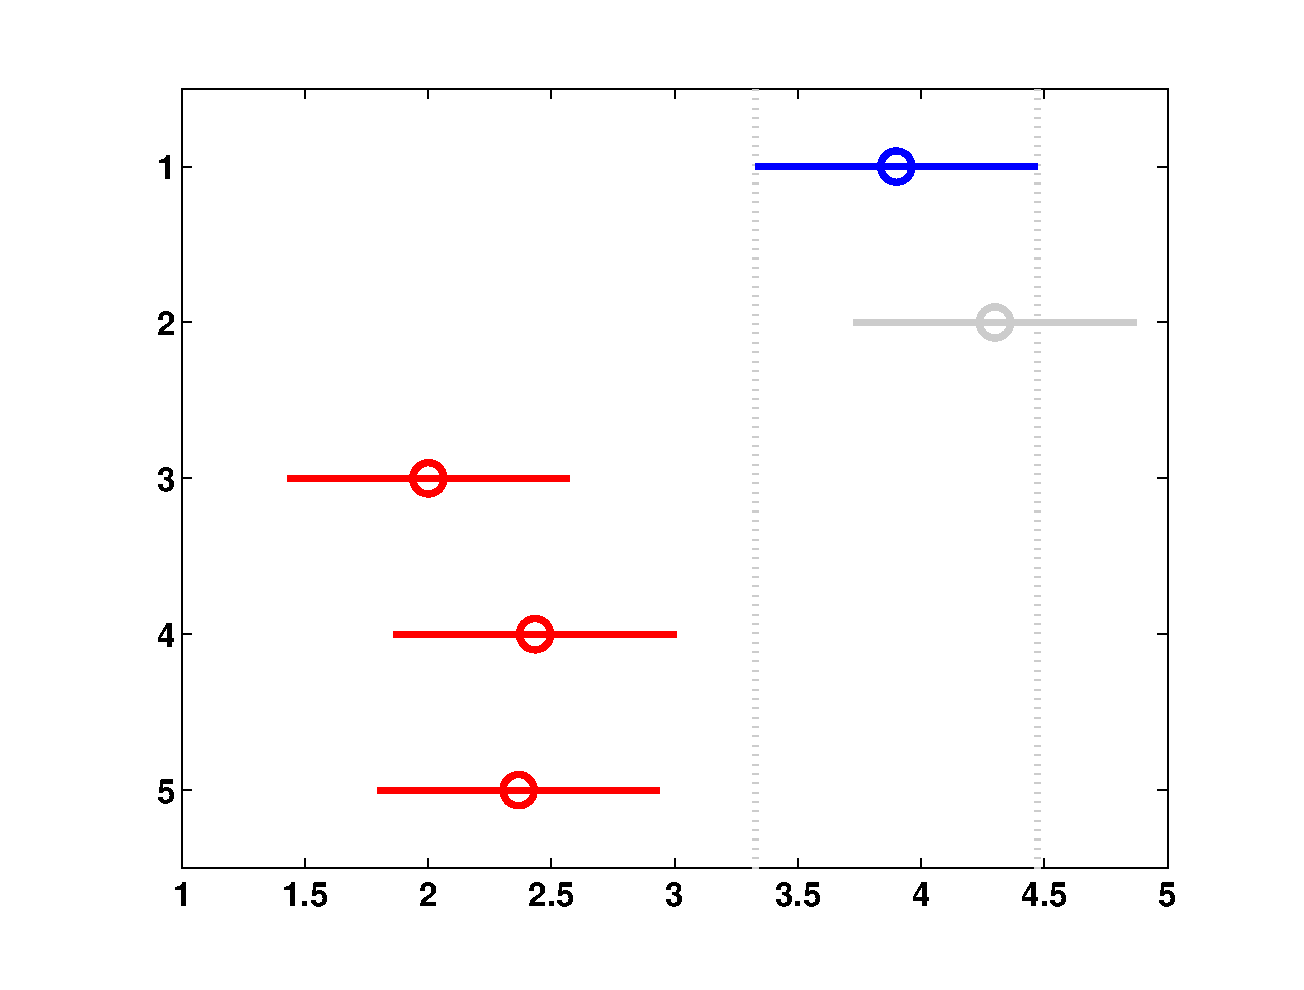
\includegraphics[width=\linewidth]{Figures/NMELA_FB_P3}
		\caption{MCE3} \label{fig:M3} 
	\end{subfigure}
	\begin{subfigure}[b]{0.49\linewidth}
		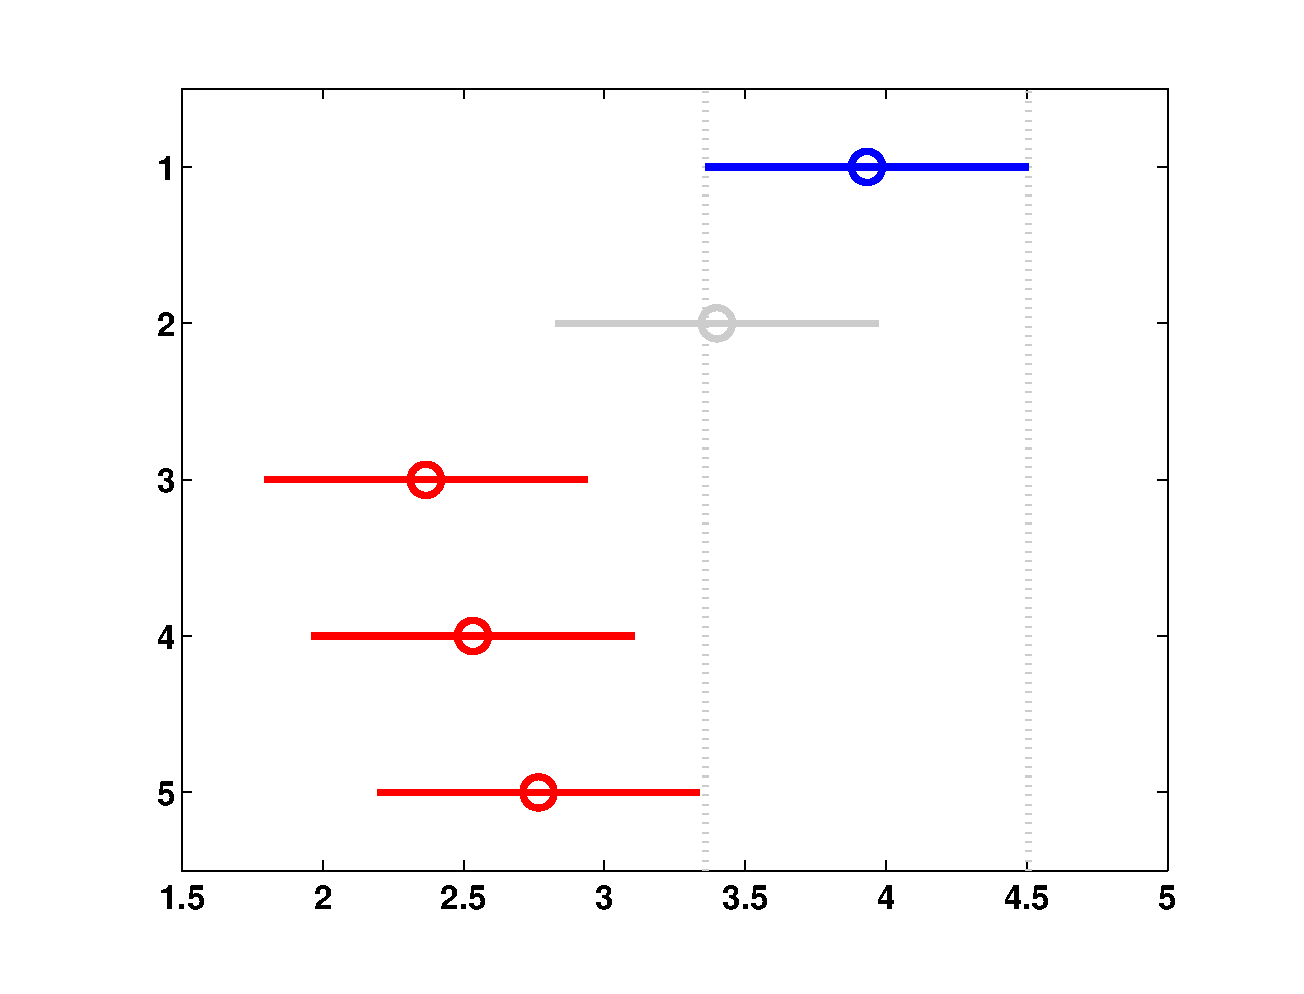
\includegraphics[width=\linewidth]{Figures/NMELA_FB_P4}
		\caption{GCE1} \label{fig:M4} 
	\end{subfigure}
	\begin{subfigure}[b]{0.49\linewidth}
		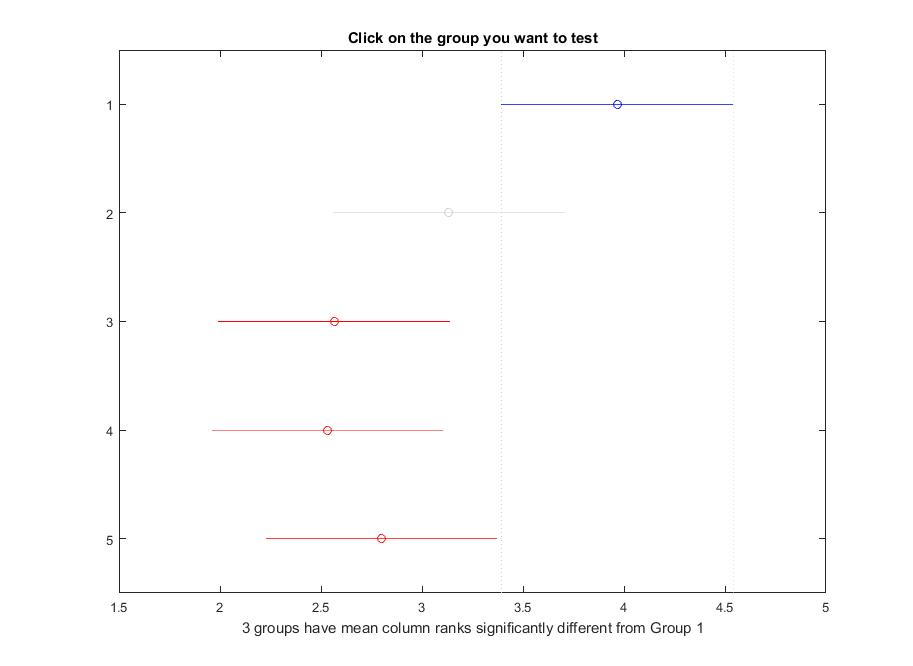
\includegraphics[width=\linewidth]{Figures/NMELA_FB_P5}
		\caption{GCE2} \label{fig:M4} 
	\end{subfigure}
	\caption{Resultados de las pruebas de Bonferroni-Dunn para las variantes NMELA y NM en los tres casos de estudio del mecanismo de cuatro barras (MCE1-3) y los dos casos de estudio del griper (GCE1-2).} \label{fig: Bonferroni-Dunn -NMELA} 
	
\end{figure}
\subsubsection{Observaciones}
En la Tabla \ref{tab:resultados NMELA} se pueden observar que las variantes NMLEA obtienen los mejores resultados en todas las medidas de estadística descriptiva y son capaces de acercase, igualar o superar en el mejor valor de la muestra a los mínimos encontrados para estos problemas. Sin embargo las medidas de tendencia central y dispersión  se encuentran lejos de estos mínimos en la mayoría de los problemas, lo que indica la sensibilidad de estos algoritmos a los puntos iniciales. El resultado de las pruebas de Friedman y Bonferroni-Dunn indican en  todos los problemas existen diferencias significativas entre al menos una variante determinista y una variante aleatorizada. Para los problemas MCE2 y MCE3 existen diferencias significativas entre el grupo determinista marcado en azul y las versiones propuestas que se encuentran a la izquierda en el grupo rojo con las mejores jerarquías. La capacidad del método Nelder-Mead para utilizar eficazmente información proveniente de regiones lejanas al área donde se encuentra operando, fue la característica fundamental por la cual fue elegido como método de búsqueda local para el diseño de los algoritmos híbridos HNMED. 



%%%%%%%%%%%%%%%%%%%%%%%%%%%%%%%%%%%%%%%%%%%%%%%%%%%%%%%%%%%%%%%%%%%%%%%%%%%%%%%%%%%%%%%%%%%%%%%%%%%%%%%%%%%%
\subsection{Experimento B: Comparación de desempeño entre Variantes HNMED vs ED/rand/1/bin}
El primer experimento se realiza para responder preguntas de investigación básicas sobre el enfoque de hibridación propuesto:
\begin{enumerate}
	\item ¿ Son los algoritmos diseñados de acuerdo al enfoque propuesto capaces de hallar valores iguales o cercanos a los mínimos conocidos para los problemas planteados ?
	\item ¿ Con qué frecuencia son los algoritmos diseñados de acuerdo al enfoque propuesto son capaces de hallar valores iguales o cercanos a  los mínimos conocidos para los problemas planteados ?
	\item ¿ Con qué rapidez los algoritmos diseñados de acuerdo al enfoque propuesto son capaces converger a los mínimos conocidos para los problemas planteados ?
	\item ¿ Presentan los algoritmos propuestos en conjunto un desempeño significativamente mejor a la Evolución Diferencial en los problemas de optimización a resolver?
	\item ¿ Cuáles de los algoritmos propuestos presentan mejor desempeño?
\end{enumerate}
\subsubsection{Definición de medidas}
Se obtendrá para cada algoritmo una muestra de $n$ ejecuciones. Cada elemento de la muestra es el valor de la función objetivo del mejor individuo factible encontrado en la ejecución $i$ para $i= \{ 1,2,...,n\}$. Para cada muestra se obtendrá:
\begin{enumerate}
	\item \textbf{Mejor}: valor mínimo de función objetivo registrado en la muestra.
	\item \textbf{Peor}: valor máximo registrado en la muestra.
	\item \textbf{Mediana}: valor que se encuentra en el centro de la muestra ordenada. Esta medida es fundamental para evaluar el desempeño ya que el promedio puede ser afectado por valores anómalos. 
	\item \textbf{Promedio}: valor característico o tendencia central la muestra.
	\item \textbf{Desviación estándar}: grado de dispersión de las soluciones registradas en la muestra con respecto al promedio.
	\item \textbf{Gráfica de convergencia}: Presenta el valor de la función objetivo del mejor individuo en la población en cada evaluación.
    \item \textbf{Prueba de Friedman}: con nivel significancia $\alpha=0.05$ para determinar si existen diferencias significativas entre el desempeño de al menos dos de los algoritmos comparados. 
	\item \textbf{Prueba Bonferroni-Dunn}: con nivel significancia $\alpha=0.05$. Teniendo en cuenta el promedio jerarquías obtenidas en la prueba de Friedman se determina entre cuáles de los algoritmos comparados existe una diferencia significativa de desempeño.     
\end{enumerate}
\subsubsection{Planificación pre-experimental y configuración}
Para el presente experimento se generaron 6 muestras correspondientes a las 5 variantes propuestas y la  ED/rand/1/bin de tamaño $n=31$. Las ejecuciones se llevaron a cabo en una computadora con procesador AMD Athlon II X2, memoria RAM 2GB, sistema operativo Windows 7 con arquitectura de 64 bits y como entorno de programación se utilizó  MatLab R2016b. 

Para este experimento se utilizó un número fijo de evaluaciones (las utilizadas por la ED) para todos los algoritmos en comparación en cada problema de optimización según se describe en la tabla \ref{tab:Evaluaciones utilizadas por problema de optimización: Experimento B.}:

\begin{table}[]
	\centering
	\caption{Evaluaciones utilizadas por problema de optimización: Experimento B.}
	\label{tab:Evaluaciones utilizadas por problema de optimización: Experimento B.}
	\begin{tabular}{cc}
		\textbf{Problema} &   \textbf{Evaluaciones}     \\
		\hline
		MCE1   &   750030       \\
		MCE2   &   20000       \\
		MCE3   &   450018      \\
		GCE1   &   750030       \\
		GCE2   &   750030      \\
		SCE1   &   288000       \\
	\end{tabular}
\end{table}
La configuración de parámetros utilizada por las variantes HNMED y la ED es la siguiente:
\begin{enumerate}
	\item Se establece la probabilidad de cruza $CR=\{0.8, 1\}$ para ED y HNMED para todos los problemas.
	\item Se establece el factor de escala $F=\{0.3, 0.9\}$ para ED y HNMED para todos los problemas.
	\item Para las variantes HNMED se establecieron los parámetros de reflexión $\alpha=2$, expansión $\gamma=1.5$ $\beta=0.5$ para todos los problemas.
	\item El tamaño de población se estableció según la Tabla \ref{tab:Tamaño de población utilizados para cada problema en el experimento B.}. Donde el valor $NS$ se refiere a la cantidad de símpleces utilizados los cuales determinan la población para cada problema $NP=NS(N+1)$ donde $N$  es la dimensión del problema.
\end{enumerate}

\begin{table}[]
	\centering
	\caption{Tamaño de población utilizados para cada problema en el experimento B.}
	\label{tab:Tamaño de población utilizados para cada problema en el experimento B.}
	\begin{tabular}{cccc}
		& \textbf{ED/rand/1/bin }& \multicolumn{2}{l}{\textbf{HNMED}} \\
		\hline
		\textbf{Problema} & \textbf{NP}            & \textbf{NS}          & \textbf{NP}          \\
		\hline
		MCE1     & 138           & 9           & 144         \\
		MCE2     & 50            & 4           & 28          \\
		MCE3     & 138           & 7           & 140         \\
		GCE1     & 138           & 9           & 135         \\
		GCE2     & 138           & 8           & 135         \\
		SCE1     & 50            & 7           & 35         
	\end{tabular}
\end{table}

\subsubsection{Presentación de resultados}
En la Tabla \ref{tab:Resultados estadísticos obtenidos por variantes HNMED y DE/rand/1/bin  experimento B.} se muestran los resultados obtenidos en la estadísticas descriptivas para las variantes propuestas y la ED/rand/1/bin en los 6 problemas de optimización. Los resultados ganadores se resaltan en letra negrita. A pesar de que existe el análisis teórico para determinar la tasa de convergencia, los experimentos realizados se limitaron a la graficación del valor de $f(x)$ presentado por el mejor individuo factible en la población, en función del número de evaluaciones de $f(x)$ denominado $NEF$. En la Figura \ref{fig: Gráficas de convergencia para las variantes HNMED y ED/rand/1/bin} se muestran las gráficas de convergencia de la ejecución correspondiente a la mediana de la muestra. En caso del problema de la micro-red eléctrica Se grafican los valores de función objetivo correspondientes a la hora 12.   

\begin{table}
	
	\caption{Resultados estadísticos obtenidos por variantes HNMED y DE/rand/1/bin en experimento B para los seis problemas de diseño cinemático. Se marcan en negritas los mejores valores de cada medida.}\label{tab:Resultados estadísticos obtenidos por variantes HNMED y DE/rand/1/bin  experimento B.}
	
	\centering
	\resizebox{\textwidth}{!}{%
		\begin{tabular}{clcccccc} 
			\hline
			Problema              & Estadística   & HNMED-V1 & HNMED-V2 &HNMED-V3 &HNMED-V4 &HNMED-V5 & ED/rand/1/bin  \\ 
			\hline
			\multirow{6}{*}{MCE1} & Mejor        & 5.55358E-28 &5.31513E-07& \textbf{0} & 1.26218E-29&5.04871E-29 &1.7670E-28 \\
			& Peor        & 2.73815E-02 & 1.6149E+00 & 2.5685E-02 & \textbf{2.2528E-02} & 2.5749E-02 & 2.7649E-02 \\
			& Mediana     & 2.2312E-04 & 2.5478E-04  & 2.0521E-04 & 2.4414E-04 & 2.1680E-04 & \textbf{4.2746E-06 }  \\
			& Promedio    & 2.6670E-03 & 5.4682E-02  & \textbf{1.8612E-03} & 3.6684E-03 & 2.5208E-03 & 2.9850E-01  \\
			& Desv. Est.   & 7.3917E-03 & 2.8965E-01 &\textbf{ 6.2715E-03} & 7.9230E-03 & 7.1453E-03 & 8.1906E-03  \\
			\hline                      
			\multirow{6}{*}{MCE2} & Mejor        &  2.6280E-03 & 2.6280E-03 &  2.6280E-03 &  2.6280E-03 &  2.6280E-03 & 2.6280E-03 \\
			& Peor        & 2.6290E-03 &  \textbf{2.6280E-03}  &  \textbf{2.6280E-03} &  \textbf{2.6280E-03}&  \textbf{2.6280E-03 }& 2.6426E-03 \\
			& Mediana     &2.6280E-03 &  2.6280E-03 &  2.6280E-03&  2.6280E-03 & 2.6280E-03 & 2.6280E-03\\
			& Promedio    & 2.6281E-03 &\textbf{2.6280E-03 }& \textbf{ 2.6280E-03} & \textbf{2.6280E-03} &  \textbf{2.6280E-03} & 2.6288E-03 \\
			& Desv. Est.   &2.3345E-07 &\textbf{ 17600E-18}  &1.0776E-15&  3.2328E-15 &  \textbf{1.7600E-18 }& 2.7205E-06\\   
			\hline
			
			\multirow{6}{*}{MCE3} & Mejor       & 2.7496E-01 & 2.7496E-01 & 2.7496E-01 & 2.7496E-01 &  2.7496E-01 & 2.7496E-01 \\
			& Peor        & 1.3508E+01 & 1.3508E+01 & 1.3508E+01 & 1.3508E+01& 1.3508E+01 &  1.3508E+01 \\
			& Mediana     & 4.3436E-01  & 1.6290E+00& 9.1663E-01 & 6.6851E-01& 4.2346E-01 &\textbf{2.7563E-01} \\
			& Promedio    & 4.2838E+00 &  6.4180E+00& 4.7519E+00 & 5.1492E+00 & 5.5448E+00 & \textbf{1.2313E+00} \\
			& Desv. Est.  & 6.0160E+00  & 6.5415E+00& 5.9814E+00 & 6.3172E+00 & 6.4445E+00  &\textbf{3.2919E+00}\\
			\hline
			\multirow{6}{*}{GCE1} & Mejor        &2.8398E-29 & \textbf{0}          & \textbf{0}          &\textbf{0}           & \textbf{0}          &6.7147E-27 \\
			& Peor        & 3.1333E-27 & 1.7670E-27 & 6.8157E-28 & 6.3109E-29 &\textbf{5.0487E-29} & 5.9926E-20\\
			& Mediana     & 1.0302E-28 & 3.1554E-30 & 3.1554E-30 & 1.5777E-30 & \textbf{0}& 3.9485E-23 \\
			& Promedio    & 1.2272E-27 & 8.7721E-29  & 4.3439E-29 &1.1359E-29 & \textbf{7.9937E-30 }& 3.4957E-21 \\
			& Desv. Est.  & 97794E-28 & 3.2234E-28  & 1.2753E-28 & \textbf{1.6873E-29 }& 1.7728E-29  & 1.2077E-20\\
			\hline
			
			\multirow{6}{*}{GCE2} & Mejor        & \textbf{1.1385E-01 }& \textbf{1.1385E-01}  & \textbf{1.1385E-01 }& \textbf{1.1385E-01}& \textbf{1.1385E-01} & 1.1388E-01 \\
			& Peor        & 1.9561E-01 & 1.5875E-01  & 1.5965E-01& 1.5976E-01 & \textbf{1.5751E-01} & 1.6075E-01\\
			& Mediana     & 1.1995E-01& 1.1440E-01  & 1.5199E-01 & 1.1410E-01 & \textbf{1.1385E-01} & 1.1447E-01 \\
			& Promedio    & 1.3600E-01& 1.3166E-01  & 1.3561E-01 & 1.2979E-01 & 1.2940E01 & \textbf{1.2080E-01} \\
			& Desv. Est.   &2.4766E-02 & 2.0980E-02  & 2.1283E-02 & 1.9838E-01& 1.9926E-02 & \textbf{1.4713E-02} \\
			\hline                      
			\multirow{6}{*}{SCE1} & Mejor        & -5.7049E+05&	\textbf{-5.7741E+05}&	-5.6195E+05&	-5.4519E+05&-5.3238E+05 &-5.3206E+05 \\
			& Peor        & -5.1016E+05&	-5.2146E+05&	-5.2772E+05&	-5.3071E+05&	\textbf{-5.3198E+05} &-5.3204E+05 \\
			& Mediana     & -5.3059E+05&	-5.3158E+05&	-5.3135E+05&	-5.3184E+05&	\textbf{-5.3209E+05 }& -5.3205E+05 \\
			& Promedio    & -5.3174E+05&	\textbf{-5.3339E+05}&	-5.3308E+05&	-5.3236E+05&	-5.3214E+05& -5.3205E+05\\
			& Desv. Est.   & 1.1452E+04&	9.2013E+03&	7.1985E+03&	2.4432E+03&	1.0096E+02& \textbf{3.3010E+00}\\
			\hline
			
			
			
			
			
			
			
		\end{tabular}
	}
\end{table}

%Grafica_Convergencia_Problema

\begin{figure}
	\centering
	\begin{subfigure}[b]{0.49\linewidth}
		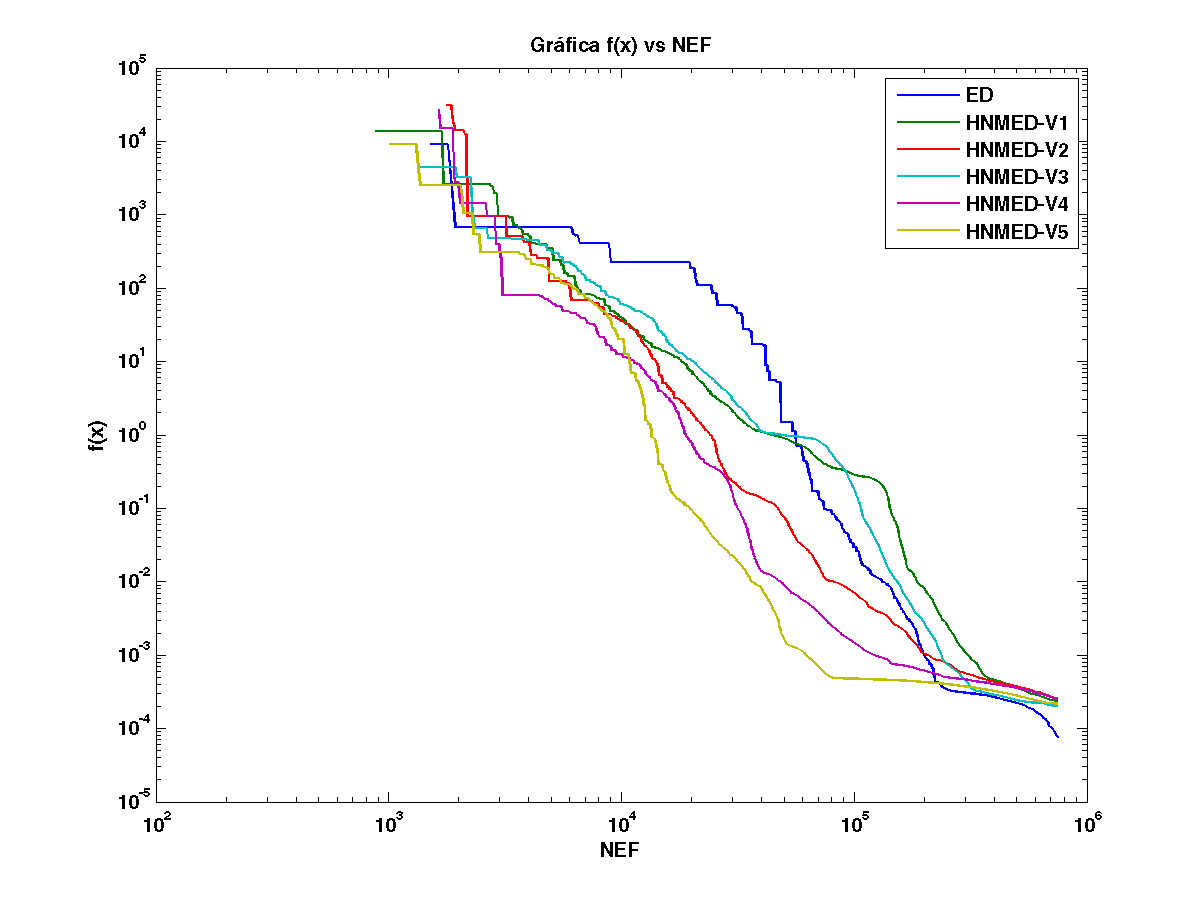
\includegraphics[width=\linewidth]{Figures/Grafica_Convergencia_Problema_1}
		\caption{MCE1} \label{fig:M1} 
	\end{subfigure}
	\begin{subfigure}[b]{0.49\linewidth}
		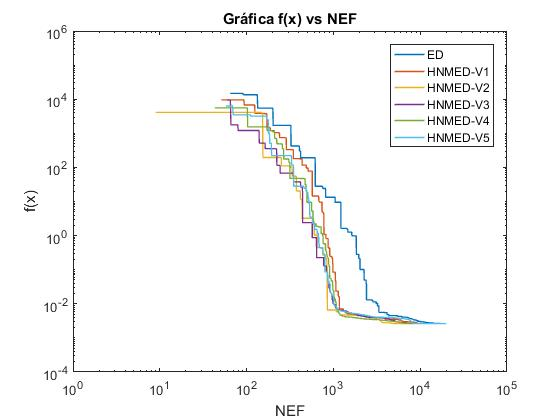
\includegraphics[width=\textwidth]{Figures/Grafica_Convergencia_Problema_2}
		\caption{MCE2} \label{fig:M2} 
	\end{subfigure}
	\begin{subfigure}[b]{0.49\linewidth}
		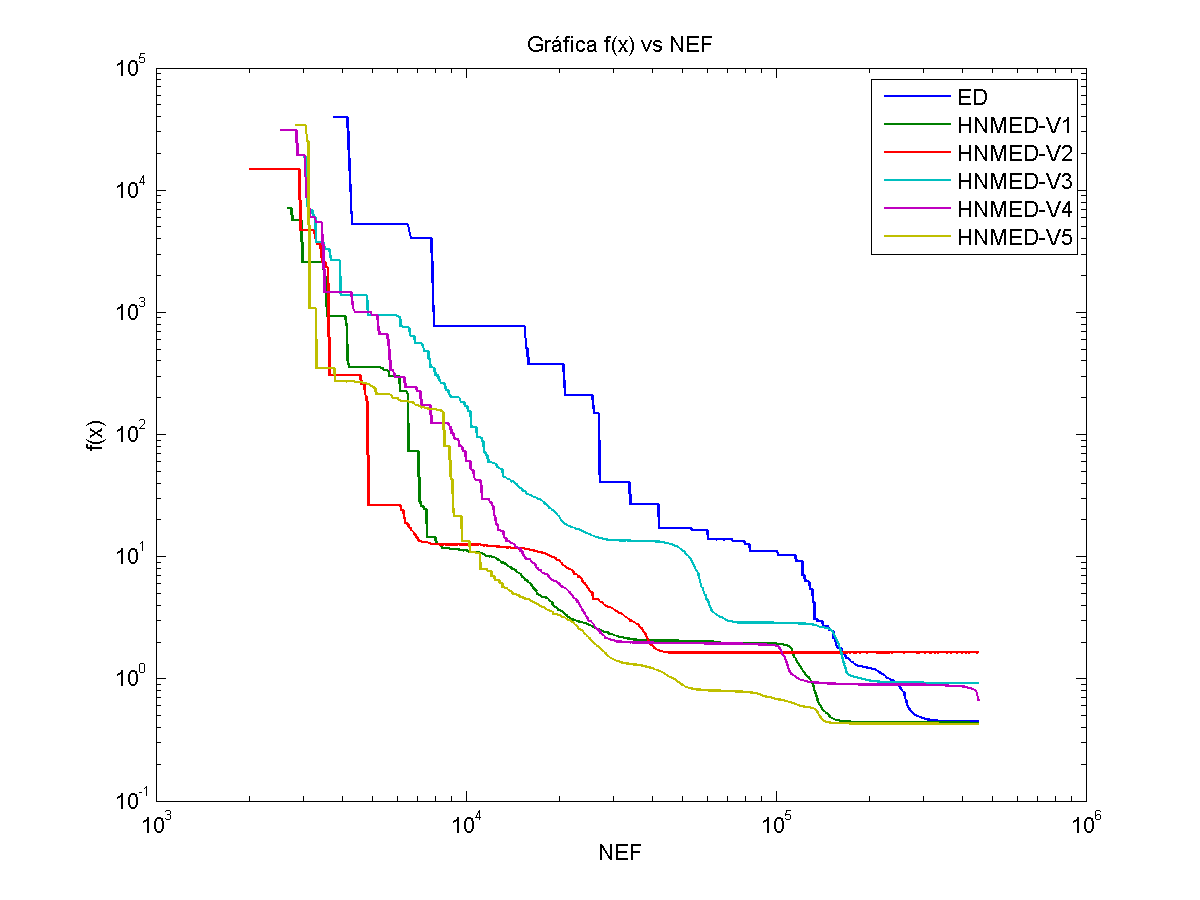
\includegraphics[width=\linewidth]{Figures/Grafica_Convergencia_Problema_3}
		\caption{MCE3} \label{fig:M3} 
	\end{subfigure}
	\begin{subfigure}[b]{0.49\linewidth}
		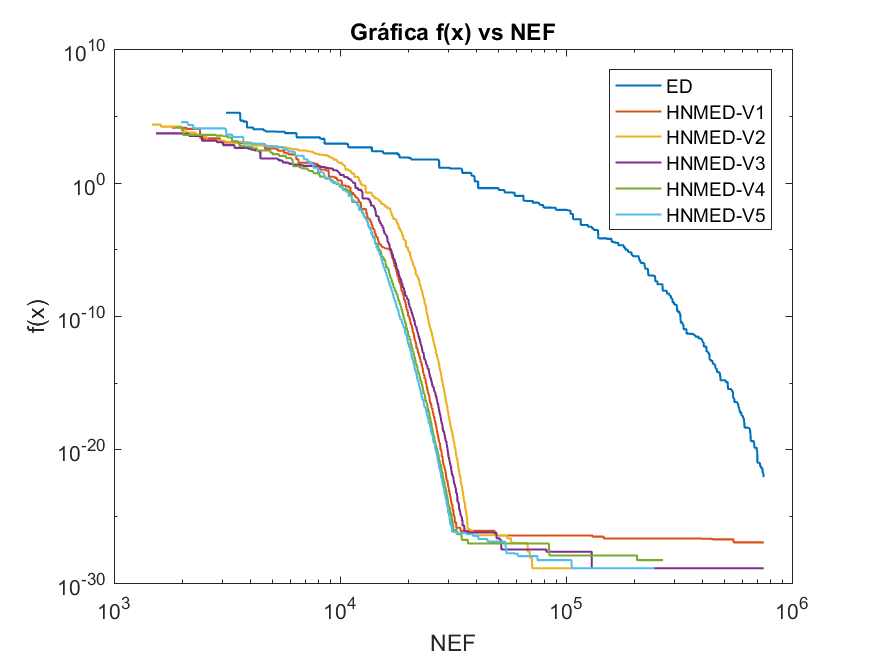
\includegraphics[width=\linewidth]{Figures/Grafica_Convergencia_Problema_4}
		\caption{GCE1} \label{fig:G1} 
	\end{subfigure}
	\begin{subfigure}[b]{0.49\linewidth}
		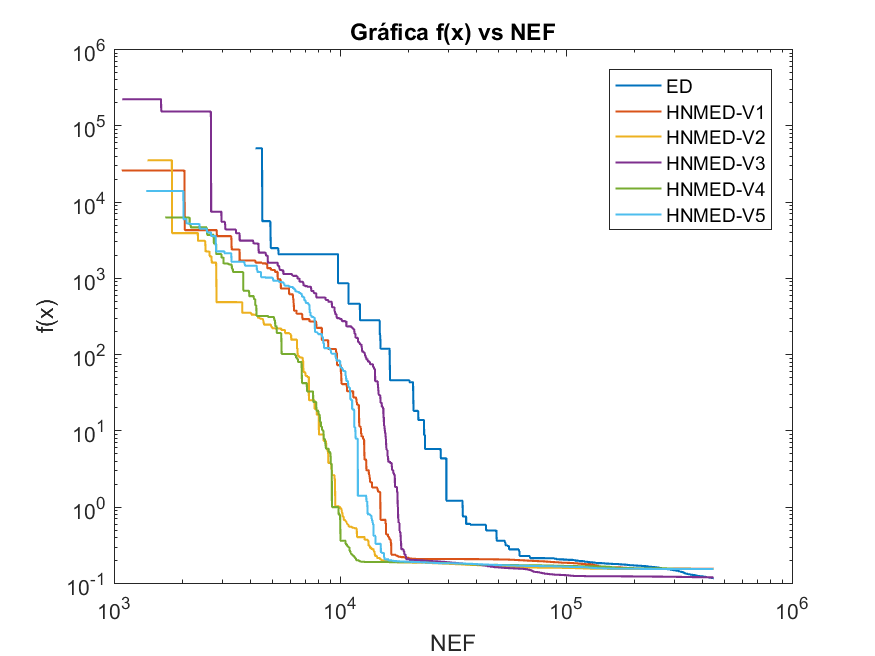
\includegraphics[width=\linewidth]{Figures/Grafica_Convergencia_Problema_5}
		\caption{GCE2} \label{fig:G2} 
	\end{subfigure}
	\begin{subfigure}[b]{0.49\linewidth}
		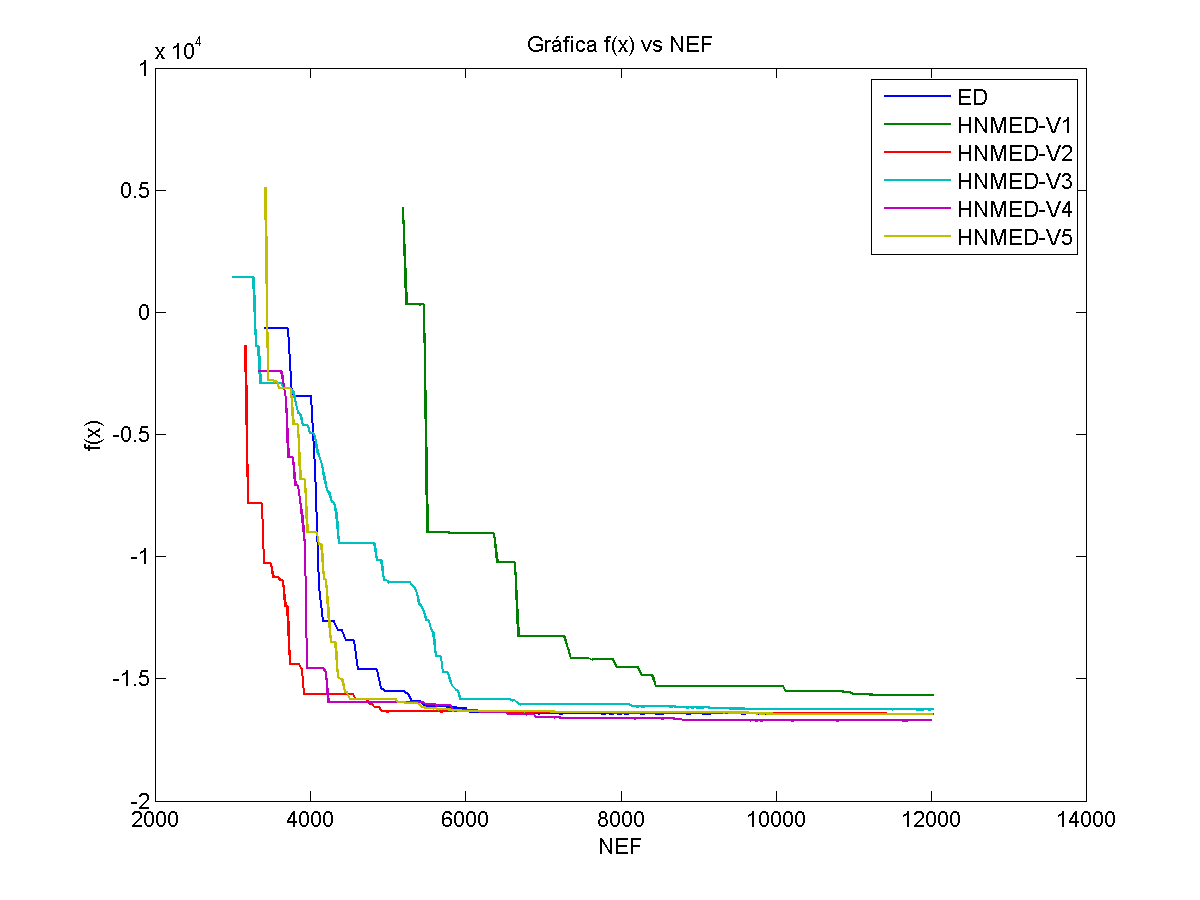
\includegraphics[width=\linewidth]{Figures/Grafica_Convergencia_Problema_6}
		\caption{SCE2} \label{fig:S1} 
	\end{subfigure}
	\caption{Gráficas de convergencia obtenidas por las variantes HNMED y ED/rand/1/bin en el experimento B} \label{fig: Gráficas de convergencia para las variantes HNMED y ED/rand/1/bin} 
	
\end{figure}
En la Tabla \ref{tab:Resultados Firedman obtenidos por variantes HNMED y DE/rand/1/bin  experimento B.} se presentan las jerarquías promedios obtenidas por los algoritmos, los valores $p$ y la aceptación o rechazo de la hipótesis obtenidas en la prueba de Firedman en cada uno de los problemas de optimización. Se resaltan en letra negrita las promedios de jerarquías ganadores.

Teniendo en cuenta los resultados de la prueba de Friedman, la Figura \ref{fig: Resultados de las pruebas de Bonferroni-Dunn para las variantes HNMED vs ED/rand/1/bin en el Experitmento B} la prueba post hoc de Bonferroni-Dunn para los 6 problemas. En las gráficas, el eje vertical presenta las etiquetas dadas a cada algoritmo y el horizontal las jerarquías promedios. Los círculos corresponden a la asignación de la etiqueta $L_j$ con el promedio jerarquía  $R_j$. Las lineas son los intervalos de confianza calculados por la prueba. Las etiquetas están asignadas de la siguiente forma: a la ED le corresponde el número 1 y a las variantes HNMED desde V1 a V5 les corresponden los números del 2 al 6 respectivamente.

Cuando los intervalos de confianza de dos muestras no se traslapan indica que se rechaza la sub-hipótesis nula y por lo tanto que existen diferencias significativas entre los algoritmos que describen dichas muestras. En las figuras presentadas los promedios de jerarquía e intervalos de confianza entre los cuales existen diferencias significativas se dibujan con colores diferentes (azul y rojo) para hacer más legible la gráfica.     
%%%%%%%%%%%%%%%%%%%%%%

\begin{table}
	\centering
	\caption{Resultados de la prueba de Friedman en variantes HNMED y DE/rand/1/bin en experimento B para los seis problemas de diseño mecatrónico}
	\label{tab:Resultados Firedman obtenidos por variantes HNMED y DE/rand/1/bin  experimento B.}
	\resizebox{\textwidth}{!}{%{0.3132\textheight}{%
		\begin{tabular}{lccccc}
			\hline
			Problema              & Algoritmo     & Jerarquía promedio &Valor de $p$        & $H_0$                           & $H_1$             \\
			\hline  
			\multirow{6}{*}{MCE1} & HNMED-V1      &3.6451E+00          &\multirow{6}{*}{8.1173E-01}  & \multirow{6}{*}{Aceptada}& \multirow{6}{*}{Rechazada} \\
			& HNMED-V2      &  3.8709E+00        &                    &                          &                            \\
			& HNMED-V3      &  3.3870E+00        &                    &                          &                            \\
			& HNMED-V4      &  3.4516E+00        &                    &                          &                            \\
			& HNMED-V5      &  3.4193E+00        &                    &                          &                            \\
			& ED/rand/1/bin &\textbf{3.2258E+00} &                    &                          &                            \\
			\hline  
			\multirow{6}{*}{MCE2} & HNMED-V1      & 3.5322E+00         & \multirow{6}{*}{1.3277E-26} & \multirow{6}{*}{Rechazada}& \multirow{6}{*}{Aceptada} \\
			& HNMED-V2      &\textbf{2.8387E+00 }&                    &                          &                            \\
			& HNMED-V3      & 2.9193E+00         &                    &                          &                            \\
			& HNMED-V4      & 2.9032E+00         &                    &                          &                            \\
			& HNMED-V5      &\textbf{2.8387E+00 }&                    &                          &                            \\
			& ED/rand/1/bin &   5.9677E+00       &                    &                          &                            \\
			\hline
			
			\multirow{6}{*}{MCE3} & HNMED-V1      &  3.5161E+00        & \multirow{6}{*}{9.4985E-01}  & \multirow{6}{*}{Aceptada}& \multirow{6}{*}{Rechazada} \\
			& HNMED-V2      & 3.7258E+00         &                    &                          &                            \\
			& HNMED-V3      & 3.5483E+00         &                    &                          &                            \\
			& HNMED-V4      & 3.5483E+00         &                    &                          &                            \\
			& HNMED-V5      &  3.5800E+00         &                    &                          &                            \\
			& ED/rand/1/bin & \textbf{3.2258E+00}    &                    &                          &                            \\
			\hline  
			\multirow{6}{*}{GCE1} & HNMED-V1      &   4.9000E+00       & \multirow{6}{*}{1.3365E-22}  & \multirow{6}{*}{Rechazada}& \multirow{6}{*}{Aceptada} \\
			& HNMED-V2      &   2.7333E+00       &                    &                          &                            \\
			& HNMED-V3      &   2.7333E+00       &                    &                          &                            \\
			& HNMED-V4      &   2.5000E+00       &                    &                          &                            \\
			& HNMED-V5      &\textbf{2.1333E+00} &                    &                          &                            \\
			& ED/rand/1/bin &   6.0000E+00       &                    &                          &                            \\
			\hline  
			\multirow{6}{*}{GCE2} & HNMED-V1      &  4.0967E+00        & \multirow{6}{*}{1.0989E-01}  & \multirow{6}{*}{Aceptada}& \multirow{6}{*}{Rechazada} \\
			& HNMED-V2      &  3.4032E+00        &                    &                          &                            \\
			& HNMED-V3      &  3.8387E+00        &                    &                          &                            \\
			& HNMED-V4      &  3.0483E+00        &                    &                          &                            \\
			& HNMED-V5      & \textbf{2.9677E+00}      &                    &                          &                            \\
			& ED/rand/1/bin & 3.0322E+00&                    &                          &                            \\
			\hline  
			
			\multirow{6}{*}{SCE1} & HNMED-V1      & 3.8709E+00                   & \multirow{6}{*}{ 1.7205E-03 }  & \multirow{6}{*}{Rechazada}& \multirow{6}{*}{Aceptada} \\
			& HNMED-V2      & 3.7741E+00                   &                    &                          &                            \\
			& HNMED-V3      & 4.3225E+00                   &                    &                          &                            \\
			& HNMED-V4      & 3.4516E+00                   &                    &                          &                            \\
			& HNMED-V5      & \textbf{2.4193E+00 }         &                    &                          &                            \\
			& ED/rand/1/bin &3.1612E+00 &                  &                    &                            \\
			
		\end{tabular}
	}
\end{table}

% Pruebas de Bunferroni

\begin{figure}
	\centering
	\begin{subfigure}[b]{0.49\linewidth}
		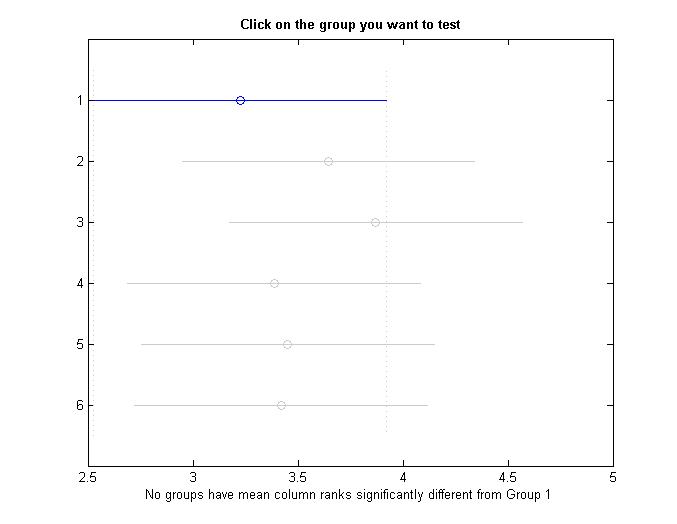
\includegraphics[width=\linewidth]{Figures/Bonferroni_HNMED_VS_ED_P1}
		\caption{MCE1} \label{fig:Bon_M1} 
	\end{subfigure}
	\begin{subfigure}[b]{0.49\linewidth}
		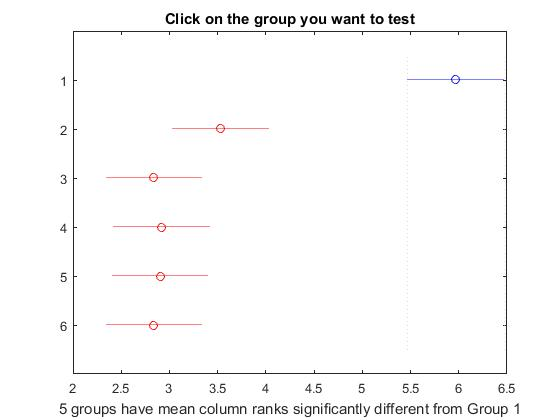
\includegraphics[width=\textwidth]{Figures/Bonferroni_HNMED_VS_ED_P2}
		\caption{MCE2} \label{fig:Bon_M2} 
	\end{subfigure}
	\begin{subfigure}[b]{0.49\linewidth}
		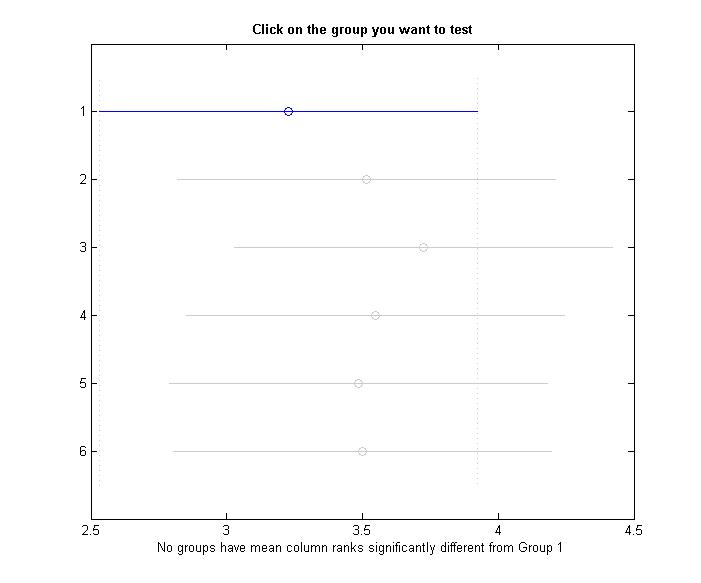
\includegraphics[width=\linewidth]{Figures/Bonferroni_HNMED_VS_ED_P3}
		\caption{MCE3} \label{fig:Bon_M3} 
	\end{subfigure}
	\begin{subfigure}[b]{0.49\linewidth}
		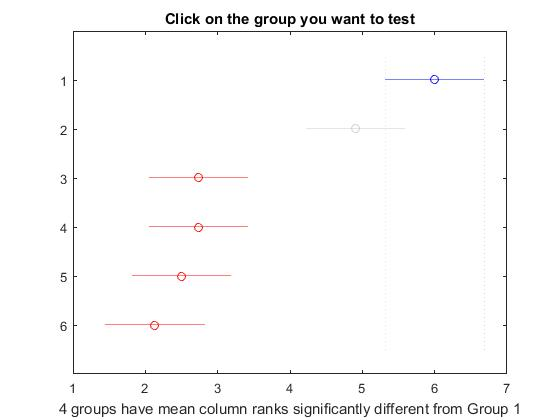
\includegraphics[width=\linewidth]{Figures/Bonferroni_HNMED_VS_ED_P4}
		\caption{GCE1} \label{fig:Bon_G1} 
	\end{subfigure}
	\begin{subfigure}[b]{0.49\linewidth}
		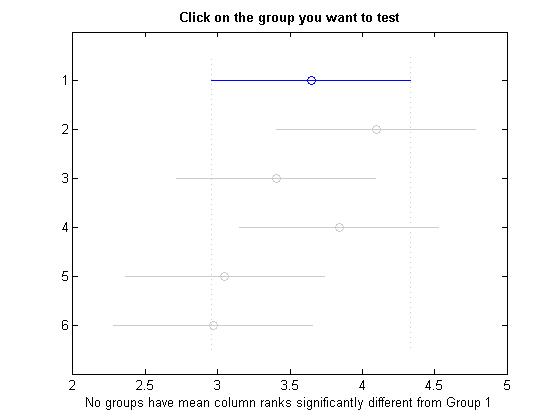
\includegraphics[width=\linewidth]{Figures/Bonferroni_HNMED_VS_ED_P5}
		\caption{GCE2} \label{fig:Bon_G2} 
	\end{subfigure}
	\begin{subfigure}[b]{0.49\linewidth}
		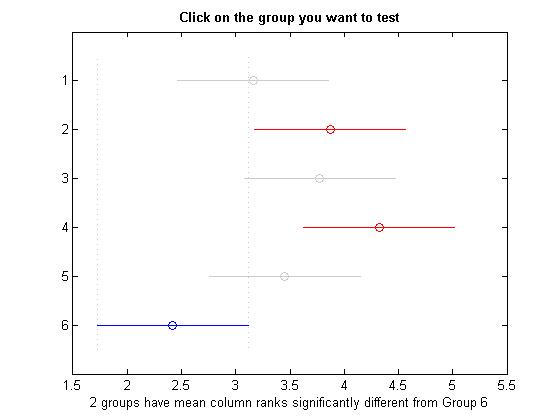
\includegraphics[width=\linewidth]{Figures/Bonferroni_HNMED_VS_ED_P6}
		\caption{SCE1} \label{fig:Bon_S1} 
	\end{subfigure}
	\caption{Resultados de las pruebas de Bonferroni-Dunn para las variantes HNMED vs ED/rand/1/bin en el Experitmento B} \label{fig: Resultados de las pruebas de Bonferroni-Dunn para las variantes HNMED vs ED/rand/1/bin en el Experitmento B} 
	
\end{figure}
%


\subsubsection{Observaciones}
Los resultados obtenidos por en la estadística descriptiva responde la primera pregunta de investigación planteada para el experimento B; ya que en efecto, las variantes propuestas son capaces de hallar valores iguales o mejores a los mínimos conocidos para todos los problemas de optimización a resolver. Las observaciones por cada problema son las siguientes:
\begin{enumerate}
	\item \textbf{MCE1}: Las variantes HNMED superan a la ED en las medidas de mejor y peor solución, promedio y desviación estándar. Ninguna logra superar el valor de la mediana de la ED. La variante HNMED con mejores resultados es V3.
	\item \textbf{MCE2}: las variantes HNMED superan a la ED en todas las medidas. La variante con mejores resultados es V5.
	\item \textbf{MCE3}: Se iguala a la ED en la mejor y peor solución de la muestra. La ED supera a las variantes HNMED en los valores de mediana, promedio y desviación estándar.La variante con mejores resultados es la V3.
	\item \textbf{GCE1}: las variantes Se supera a la ED en todas las medidas. HNMED-V5 presenta los mejores resultados.
	\item \textbf{GCE2}: Todas las variantes superan a la ED en su mejor y peor solución, excepto HNMED-V1 . Sólo HNMED-V5 (variante con mejores resultados)supera la mediana de la ED la cual prevalece en las demás medidas (promedio y desviación estándar).
	\item \textbf{SCE1}: Todas las variantes superan a la ED en el mejor resultado, siendo HNMED-V5 la que logra superar a la ED en las medidas de promedio y mediana. 
\end{enumerate}
De forma general, las variantes propuestas presentan mejores valores de las medidas de tendencia central en la mayoría de los problemas y valores modestos de desviación estándar lo que indica cierta sensibilidad a la distribución inicial de la población. Se destacan además las medida de la mejor solución de la muestra en la cual las variantes siempre obtienen resultados iguales (para MCE2 y MCE3) o mejores (MCE1,GCE1,GCE2,SCE1) a la ED. Esto se debe a la capacidad de explotación de las instancias del método Nelder Mead.

En la Figura \ref{fig: Gráficas de convergencia para las variantes HNMED y ED/rand/1/bin} se observa que, para todos los problemas las curvas descritas por las variantes HNMED se encuentran por debajo a las de ED/rand/1/bin. Esto significa que todas las versiones pueden obtener resultados competitivos en un menor número de evaluaciones. También se puede observar que las curvas dadas por los algoritmos propuestos se encuentran ligeramente corridas a la izquierda, lo que indica que son capaces de encontrar individuos factibles en iteraciones tempranas. Este comportamiento se debe a la capacidad del simplex de muestrear el espacio de búsqueda con pocas evaluaciones. Es importante destacar que con los resultados obtenidos se demuestran dos aspectos principales robustez y eficiencia del enfoque propuesto de forma general. 
En la Tabla \ref{tab:Resultados Firedman obtenidos por variantes HNMED y DE/rand/1/bin  experimento B.} se observan los resultados obtenidos en la prueba de friedman para cada problema:
\begin{enumerate}
	\item \textbf{MCE1}: El mejor promedio de jerarquía obtenido corresponde a la ED. Sin embargo, se acepta la hipótesis nula con un valor de $p=8.1173E-01$ Esto significa que a pesar de que la ED obtiene mejores resultados en este problema,  no se puede afirmar que son significativamente mejores y por lo tanto su desempeño es similar al de las variantes HNMED. La mejor jerarquía obtenida por las variantes HNMED corresponden a V5.
	\item \textbf{MCE2}: El algoritmo HNMED-V5  obtiene el mejor promedio de jerarquía. Además, todas las versiones HNMED obtienen una mejor jerarquía promedio con respecto a la ED. En este caso se rechaza la hipótesis nula con valor de $p=1.3277E-26$. En este problema se evidencia un desempeño significativamente mejor por parte de las 5 variantes propuestas en comparación con la ED.
	\item \textbf{MCE3}: La ED/rand/1/bin alcanza el mejor promedio de jerarquía. No obstante, se acepta la hipótesis nula con valor de $p=9.4985E-01$. Al igual que en la prueba para el problema MCE1 se concluye que existe un desempeño similar entre todos los algoritmos comparados.
	\item \textbf{GCE1}: De forma similar al problema MCE1 todas las variantes HNMED obtienen mejor jerarquía respecto a la ED, siendo la V5 el algoritmo ganador. La hipótesis nula se rechaza concluyendo que las versiones V5 se comportan significativamente mejor que la ED.
	\item \textbf{GCE2}: EL algoritmo ganador es HNMED-V5. Todas las versiones HNMED obtienen mejores jerarquías que la ED  a excepción de la V1. En es te caso la hipótesis nula se acepta por lo tanto no se confirma que existen diferencias significativas entre el desempeño de las variantes ganadoras y la ED. 
	\item \textbf{SCE1}: En este caso se rechaza la hipótesis nula con valor de $p=1.7205E-03$, siendo HNMED-V5 el algoritmo con mejor promedio de jerarquía. Sin embargo, como se puede observar en la Subfigura F de la Figura \ref{fig: Resultados de las pruebas de Bonferroni-Dunn  para las variantes HNMED y ED/rand/1/bin}, las diferencias significativas se encuentran entre HNMED-V5 y las variantes V1 y V2.   
\end{enumerate}
De forma general se observa un desempeño competitivo de las variantes propuestas, obteniéndose resultados significativamente mejores en 2 de problemas y desempeño similar el resto con respecto a la ED/rand/1/bin. La variante HNMED-V5 consigue el mejor desempeño de forma general la cual obtiene mejor promedio de jerarquías en 4 de los 6 problemas de optimización. Los peores promedios de jerarquía se obtienen en los problemas MCE1,MCE3 y GCE2 los cuales presentan mayor dimensión, restricciones y complejidad de la función. A pesar de que las variantes propuestas ganan en rapidez de convergencia, heredan en cierta medida las deficiencias del método de búsqueda local cuyas operaciones están destinadas a la explotación. Por tanto, se presenta un decremento del desempeño para problemas de mayor dimensionailidad  aunque este no es significativo.



%%%%%%%%%%%%%%%%%%%%%%%%%%%%%%%%%%%%%%%%%%%%%%%%%%%%%%%%%%%%%%%%%%%%%%%%%%%%%%%%%%%%%%%%%%%%%%





\subsection{Experimentos C : Comparación de Variantes HNMED vs ED con reducción del número de evaluaciones}
Los experimentos D y E se realizan para conocer de forma exacta el número de evaluaciones en las que las variantes propuestas presentan un desempeño competitivo en comparación con la ED/rand/1/bin. Con la realización de estos experimentos se reúne la información necesaria sobre las variables contempladas en la hipótesis de investigación (calidad de resultados y rapidez) para concluir una aceptación o rechazo de la misma.  

\subsubsection{Definición de medidas}
Se obtiene para cada algoritmo una muestra de $n=31$ ejecuciones.Para cada problema las observaciones en la muestra corresponden a el valor de la función objetivo del mejor individuo factible encontrado por el algoritmo $A_i$en la ejecución $j$ para $j= \{ 1,2,...,n\}$. Se aplicarán al conjunto de muestras las siguientes pruebas de estadística descriptiva e inferencial:
\begin{enumerate}

		\item \textbf{Estadística descriptiva}: Se obtiene la la mejor y peor solución, mediana, promedio y desviación estándar de las muestras
		\item \textbf{Tasa de convergencia}: Se presenta la gráfica de convergencia correspondiente a la mediana de la muestra para cada algoritmo en comparación.
		\item \textbf{Prueba de Friedman}: con nivel significancia $\alpha=0.05$ para determinar si existen diferencias significativas entre el desempeño de al menos dos de los algoritmos comparados. 
		\item \textbf{Prueba Bonferroni-Dunn}: con nivel significancia $\alpha=0.05$ para determina entre cuáles de los algoritmos comparados existe una diferencia significativa de desempeño.

\end{enumerate}
\subsubsection{Planificación pre-experimental y configuración}
Para este experimento se mantuvo el número de evaluaciones realizadas por la ED según se describe en la literatura. El número de evaluaciones fue reducido para cada cada uno de los algoritmos en comparación en cada problema de optimización según se describe en la Tabla \ref{tab:Evaluaciones utilizadas por problema de optimización Experimentos C.}:

\begin{table}[]
	
	\caption{Evaluaciones utilizadas por problema de optimización Experimentos C.}
	\label{tab:Evaluaciones utilizadas por problema de optimización Experimentos C.}
	\centering
	\resizebox{\textwidth}{!}{%
		\begin{tabular}{ccccccc}
			\textbf{Problema} &   ED     &HNMED-V1&HNMED-V2&HNMED-V3&HNMED-V4&HNMED-V5   \\
			\hline
			MCE1   &   750030 &500000 &400000&400000&400000&400000   \\
			MCE2   &   20000  &15000  &15000 &15000 &15000 &15000  \\
			MCE3   &   450018 &35000  &25000 &25000 &200000 &200000 \\
			GCE1   &   750030 &125000  &125000 &125000 &125000 &125000  \\
			GCE2   &   750030 &225000  &225000 &225000 &225000 &225000 \\
			SCE1   &   288000 &240000  &240000 &240000 &240000 &240000 \\
		\end{tabular}
	}
\end{table}
La configuración de parámetros utilizada por las variantes HNMED y la ED es la siguiente:
\begin{enumerate}
	\item Se establece la probabilidad de cruza $CR=\{0.8, 1\}$ para ED y HNMED para todos los problemas.
	\item Se establece el factor de escala $F=\{0.3, 0.9\}$ para ED y HNMED para todos los problemas.
	\item Para las variantes HNMED se establecieron los parámetros de reflexión $\alpha=2$, expansión $\gamma=1.05$ $\beta=0.5$ para todos los problemas.
	\item El tamaño de población utilizado se ajusta para cada algoritmo según la Tabla \ref{tab:Tamaños de población utilizados para cada problema en el Experimento C.}. Donde el valor $NS$ se refiere a la cantidad de símpleces utilizados los cuales determinan la población para cada problema $NP=NS(N+1)$ donde $N$  es la dimensión del problema.
\end{enumerate}

\begin{table}[]
	\centering
	\caption{Tamaños de población utilizados para cada problema en el Experimento C.}
	\label{tab:Tamaños de población utilizados para cada problema en el Experimento C.}
	\resizebox{\textwidth}{!}{%
		\begin{tabular}{cccccccccccc}
			& \textbf{ED/rand/1/bin } & \multicolumn{2}{l}{\textbf{HNMED-V1}}&\multicolumn{2}{l}{\textbf{HNMED-V2}} &\multicolumn{2}{l}{\textbf{HNMED-V3}} &\multicolumn{2}{l}{\textbf{HNMED-V4}} &\multicolumn{2}{l}{\textbf{HNMED-V5}}  \\
			\hline
			\textbf{Problema} & \textbf{NP}            & \textbf{NS}          & \textbf{NP}   & \textbf{NS}          & \textbf{NP} & \textbf{NS}          & \textbf{NP}& \textbf{NS}          & \textbf{NP}& \textbf{NS}          & \textbf{NP}           \\
			\hline
			MCE1     & 138           & 9           & 144 &8&128&8&128&7&112&7&112        \\
			MCE2     & 50            & 3           & 21  &4&28&4&28&3&21&3&21        \\
			MCE3     & 138           & 7           & 140 &7&140&7&140&7&140&7&140        \\
			GCE1     & 138           & 9           & 135 &9&135&9&135&9&135&9&135        \\
			GCE2     & 138           & 9           & 135 &9&135&9&135&9&135&9&135      \\
			SCE1     & 50            & 7           & 35  &7&35&7&35&7&35&7&35       
		\end{tabular}
	}
\end{table}


\subsubsection{Presentación de resultados}
La Tabla \ref{tab:Resultados estadísticos obtenidos por variantes HNMED y DE/rand/1/bin  en experimento C.} se muestran los resultados estadísticos y en la Figura \ref{fig: Gráficas de convergencia para las variantes HNMED y ED/rand/1/bin para el Experimento C} las funciones de convergencias. En la Tabla \ref{tab:Resultados de la prueba de Friedman en las variantes HNMED y DE/rand/1/bin en el experimento C para los seis problemas de diseño mecatrónico.} se presentan los resultados de la prueba de Friedman y en la Figura \ref{fig: Resultados de las pruebas de Bonferroni-Dunn para las variantes HNMED vs ED/rand/1/bin en el experimento C.} prueba post hoc de Bonferroni-Dunn para los 6 problemas correspondientes al Experimento C.
%%%%%%%%%%%%%%%%%%%%%%%%%%%%%%%%%%%%%%%%%%%%%%%%%%%%%%%%%%%%%%%%%%%%%%%%%%%%%%%%%%%%%%%%%%%%%%%%%%%


\begin{table}
	
	\caption{Resultados estadísticos obtenidos por variantes HNMED y DE/rand/1/bin en el experimento C para los seis problemas de diseño cinemático. Se marcan en negritas los mejores valores de cada medida.}\label{tab:Resultados estadísticos obtenidos por variantes HNMED y DE/rand/1/bin  en experimento C.}
	
	\centering
	\resizebox{\textwidth}{!}{%
		\begin{tabular}{clcccccc} 
			\hline
			Problema              & Estadística   & HNMED-V1    & HNMED-V2    &HNMED-V3      &HNMED-V4      & HNMED-V5     & ED/rand/1/bin  \\ 
			\hline
			\multirow{6}{*}{MCE1} & Mejor       & 5.80602E-28&	\textbf{1.26218E-29}	   &5.04871E-29  &6.31089E-29	&4.9224E-29  &1.7670E-28 \\
			& Peor        & 3.1713E-02    &2.7676E-02    & 2.9936E-02  & \textbf{2.7424E-02}   & 2.7432E-02   & 2.7649E-02 \\
			& Mediana     & 3.4667E-04    & 3.9921E-04   & 4.5762E-04  & 3.9547E-04   & 3.4607E-04   & \textbf{4.2746E-06}   \\
			& Promedio    & \textbf{3.1573E-03}    & 4.7172E-03   & 7.1235E-03   & 4.5629E-03  & 6.9630E-03   & 2.9850E-01  \\
			& Desv. Est.  & 8.7501E-03    &1.0145E-02    & \textbf{1.1201E-03}   & 4.9555E-03  & 1.1579E-03   & 8.1906E-03  \\
			& Evaluaciones & 500000(-33\%)&400000 (-46.66\%) &400000 (-46.66\%)   & 400000 (-46.66\%) & 400000 (-46.66\%)   & 750030 \\
			
			\hline
			\multirow{6}{*}{MCE2} & Mejor       & 2.6280E-03   &2.6280E-03   &2.6280E-03    & 2.6280E-03    & 2.6280E-03   &2.6280E-03 \\
			& Peor        &2.8317E-03   & \textbf{2.6280E-03 }  & \textbf{2.6280E-03  }   & \textbf{2.6280E-03}  & \textbf{2.6280E-03  } & 2.6426E-03\\
			& Mediana     & 2.6280E-03   &2.6280E-03   & 2.6280E-03    & 2.6280E-03   & 2.6280E-03   & 2.6280E-03   \\
			& Promedio    & 2.6349E-03    &\textbf{2.6280E-03 }  & \textbf{2.6280E-03  }  &\textbf{ 2.6280E-03 } & \textbf{2.6280E-03 }  & 2.6288E-03 \\
			& Desv. Est.  & 4.6798e-03    & \textbf{8.3771E-10 }&2.2862E-09    &  6.8497E-08 & 2.8769E-09   & 2.7205E-06 \\
			& Evaluaciones&\textbf{15000}(-33.3\%) &\textbf{15000}(-33.3\%)  &\textbf{15000}(-33.3\%) & \textbf{15000}(-33.3\%)  & \textbf{15000}(-33.3\%)  &20000  \\     
			
			\hline
			\multirow{6}{*}{MCE3} & Mejor       & 2.7496E-01    & 2.7527E-01   & 2.7496E-01   &2.7496E-01   & 2.7496E-01    & 2.7496E-01  \\
			& Peor        & 1.3508E+01    & 1.3508E+01   & 1.3508E+01   & 1.3508E+01   & 1.3508E+01   & 1.3508E+01 \\
			& Mediana     & 7.3675E-01   & 7.5977E+01   & 1.6433E+00  & 5.4040E-01   & 8.8976E-01   & \textbf{2.7563E-01}   \\
			& Promedio    & 5.1387E+00   & 5.6636E+00    & 5.79209E+00  & 4.6850E+00   & 5.6552E+00   & \textbf{1.2313E+00} \\
			& Desv. Est.  & 6.3164E+00   & 6.6190E+00    & 6.2649E+00   & 6.1952E+00   & 6.3652E+00   & \textbf{8.1906E-03}  \\
			& Evaluaciones&350000(-22.2\%) &250000(-44.4\%) &250000(-44.4\%)   & 225000(-50.0\%)   & \textbf{225000}(-50.0\%)  & 450018 \\
			
			
			\hline
			\multirow{6}{*}{GCE1} & Mejor       & 6.3108E-29    &\textbf{ 0 }          &\textbf{ 0   }         &\textbf{ 0}            &\textbf{ 0 }           &6.7147E-27 \\
			& Peor        &1.7951E-26    & 1.9090E-27   & 4.7773E-27   & 2.0699E-27   & \textbf{9.0876E-28}  & 5.9926E-20 \\
			& Mediana     &2.47387E-27  & 5.0487E-29   & 5.04871-29   & 5.6797E-29   & \textbf{1.2621E-29}   & 3.9485E-23  \\
			& Promedio    &3.80302E-27   &2.3248E-28    & 4.8268E-28  & 2.4801E-28   &\textbf{ 6.2396E-29 } & 3.4957E-21  \\
			& Desv. Est.  & 4.36121E-27    &4.8191E-28   &	1.1600E-27  & 4.4014E-28   &\textbf{ 1.6612E-28}   & 1.2077E-20  \\
			& Evaluaciones&\textbf{125000}(-83.3\%) &\textbf{125000}(-83.3\%) &\textbf{125000}(-83.3\%)    & \textbf{125000}(-83.3\%)    & \textbf{125000}(-83.3\%)  & 750030\\
			
			
			\hline
			\multirow{6}{*}{GCE2} & Mejor       &\textbf{1.1385E-01}&1.4713E-02&\textbf{	1.1385E-01	}&\textbf{1.1385E-01}&	\textbf{1.1385E-01 }        &1.1388E-01 \\
			& Peor        &1.89116E-01&	2.3328E-01&	1.7400E-01&	\textbf{1.5932E-01}&	1.6559E-01    &1.6075E-01 \\
			& Mediana     &1.5513E-01&	1.5417E-01&	1.1746E-01&	1.5202E-01&	1.5294E-01 & \textbf{1.1447E-01}  \\
			& Promedio    & 1.4773E-01&	1.4407E-01&	1.3132E-01&	1.3611E-01&	1.3934E-01 &\textbf{ 1.2080E-01 } \\
			& Desv. Est.  &2.1528E-02&	2.6887E-02	&2.06472E-02	&2.0660E-02	&2.0410E-02& \textbf{1.4713E-02 }\\
			& Evaluaciones &\textbf{250000}(-44.4\%) &\textbf{250000}(-44.4\%) &\textbf{250000}(-44.4\%)  & \textbf{250000}(-44.4\%)  &\textbf{200000}(-55.5\%)  &  450018 \\
			
			
			
			
			
			\hline
			\multirow{6}{*}{SCE1} & Mejor       & -5.7452E+05    & -5.7725E+05    & \textbf{-5.8217E+05}   &-5.7364E+05   & -5.3652E+05   &-5.3206E+05 \\
			& Peor        &-4.9379E+05     & -4.9669E+o5   & -5.2250E+05   & -5.2442E+05  & -5.3080E+05  & \textbf{-5.3204E+05} \\
			& Mediana     &-5.3667E+05    &-5.3083E+05   & -5.3188E+05   & -5.3175E+05   & \textbf{-5.3217E+05}  & -5.3205E+05   \\
			& Promedio    &-5.3690E+05   &-5.33062E+05   & -5.4196E+05   & -5.3292E+05   & \textbf{-5.3230E+05 }  & -5.3205E+05 \\
			& Desv. Est.  &1.9677E+04  & 1.7853E+04    & 1.9516E+04   & 7.9197E+03   & 1.0945E+03  & \textbf{3.3010E+00 } \\
			& Evaluaciones&240000 (-8.3 \%) & 240000 (-16.6 \%)  & 240000 (-16.6 \%)   & \textbf{216000} (-25.0 \%) & \textbf{216000} (-25.0 \%)&288000
			
			
			
			
			
		\end{tabular}
	}
\end{table}
\begin{figure}
	\centering
	\begin{subfigure}[b]{0.49\linewidth}
		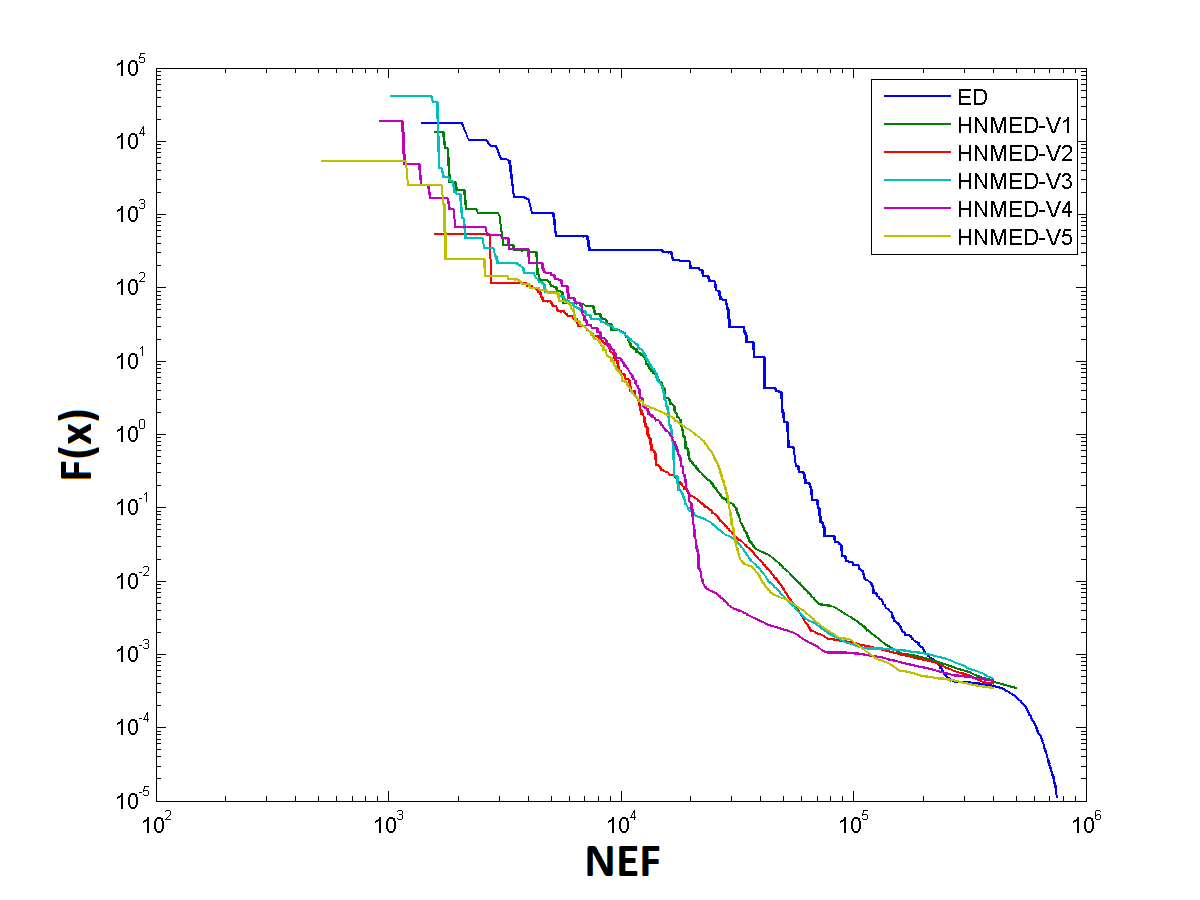
\includegraphics[width=\linewidth]{Figures/C-Grafica_Convergencia_Problema_1}
		\caption{MCE1} \label{fig:M1} 
	\end{subfigure}
	\begin{subfigure}[b]{0.49\linewidth}
		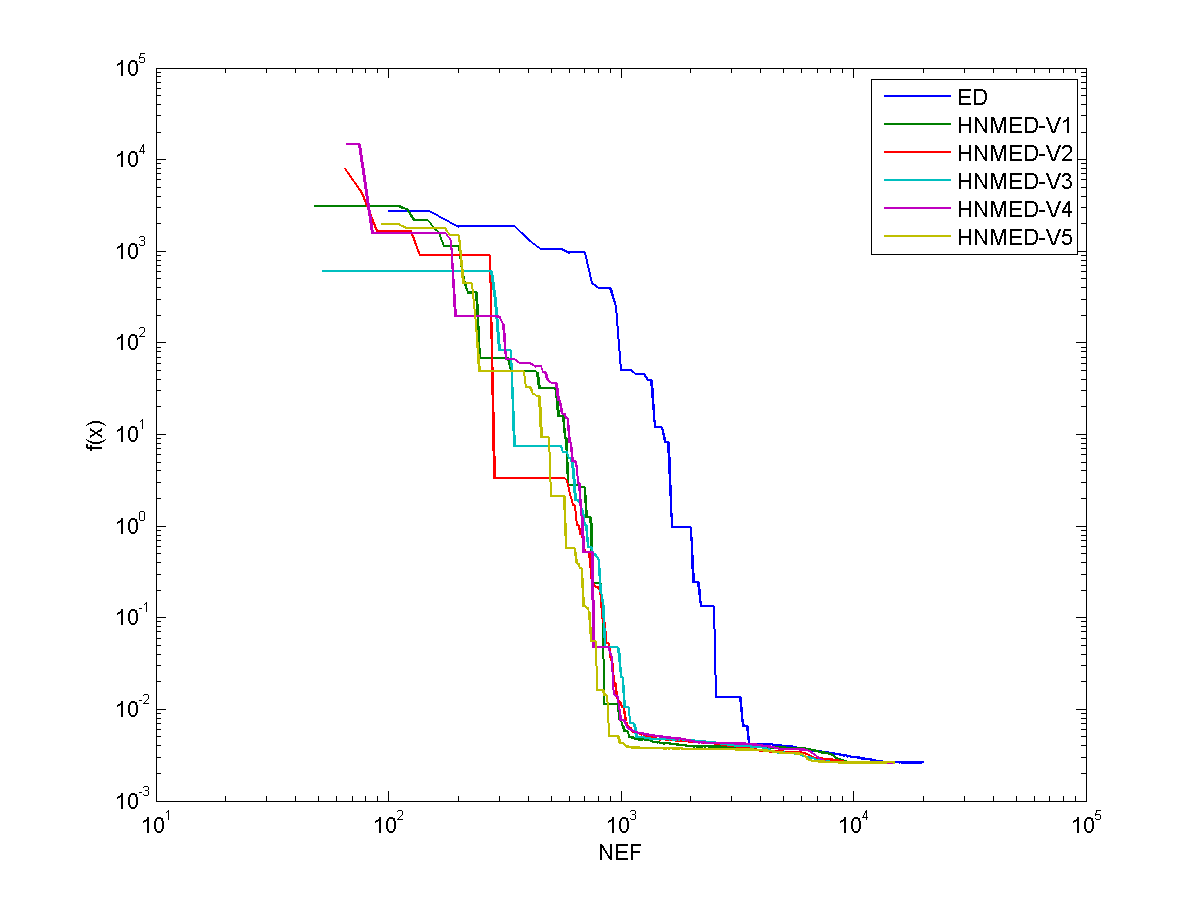
\includegraphics[width=\textwidth]{Figures/C-Grafica_Convergencia_Problema_2}
		\caption{MCE2} \label{fig:M2} 
	\end{subfigure}
	\begin{subfigure}[b]{0.49\linewidth}
		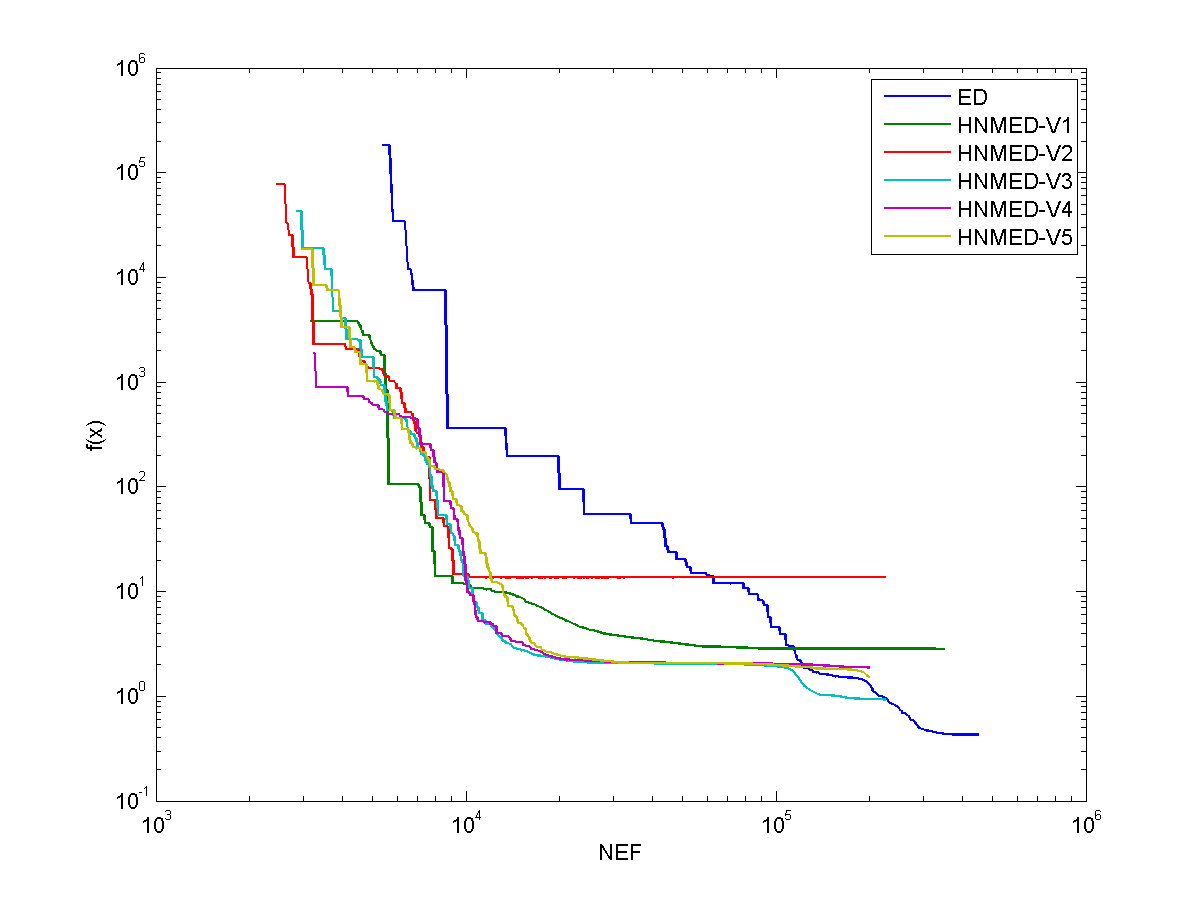
\includegraphics[width=\linewidth]{Figures/C-Grafica_Convergencia_Problema_3}
		\caption{MCE3} \label{fig:M3} 
	\end{subfigure}
	\begin{subfigure}[b]{0.49\linewidth}
		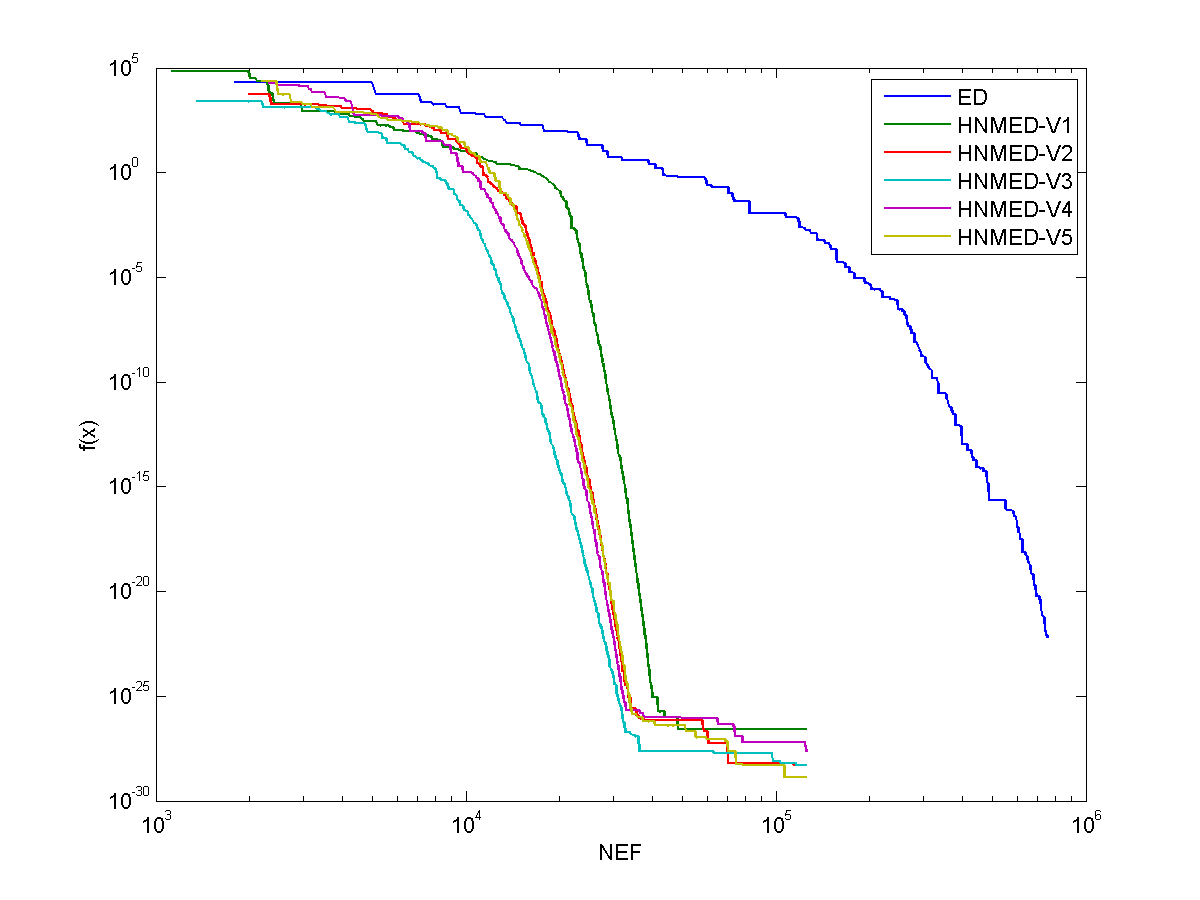
\includegraphics[width=\linewidth]{Figures/C-Grafica_Convergencia_Problema_4}
		\caption{GCE1} \label{fig:G1} 
	\end{subfigure}
	\begin{subfigure}[b]{0.49\linewidth}
		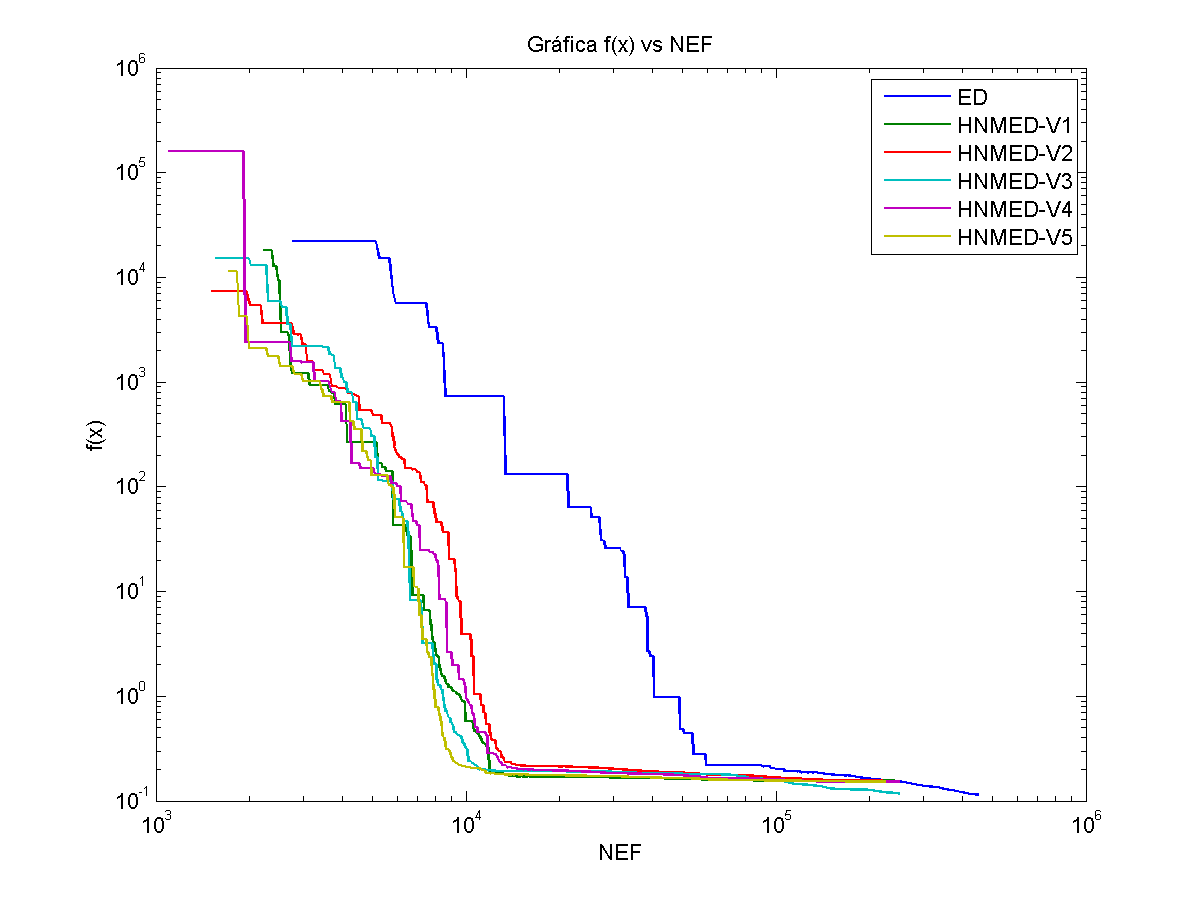
\includegraphics[width=\linewidth]{Figures/C-Grafica_Convergencia_Problema_5}
		\caption{GCE2} \label{fig:G2} 
	\end{subfigure}
	\begin{subfigure}[b]{0.49\linewidth}
		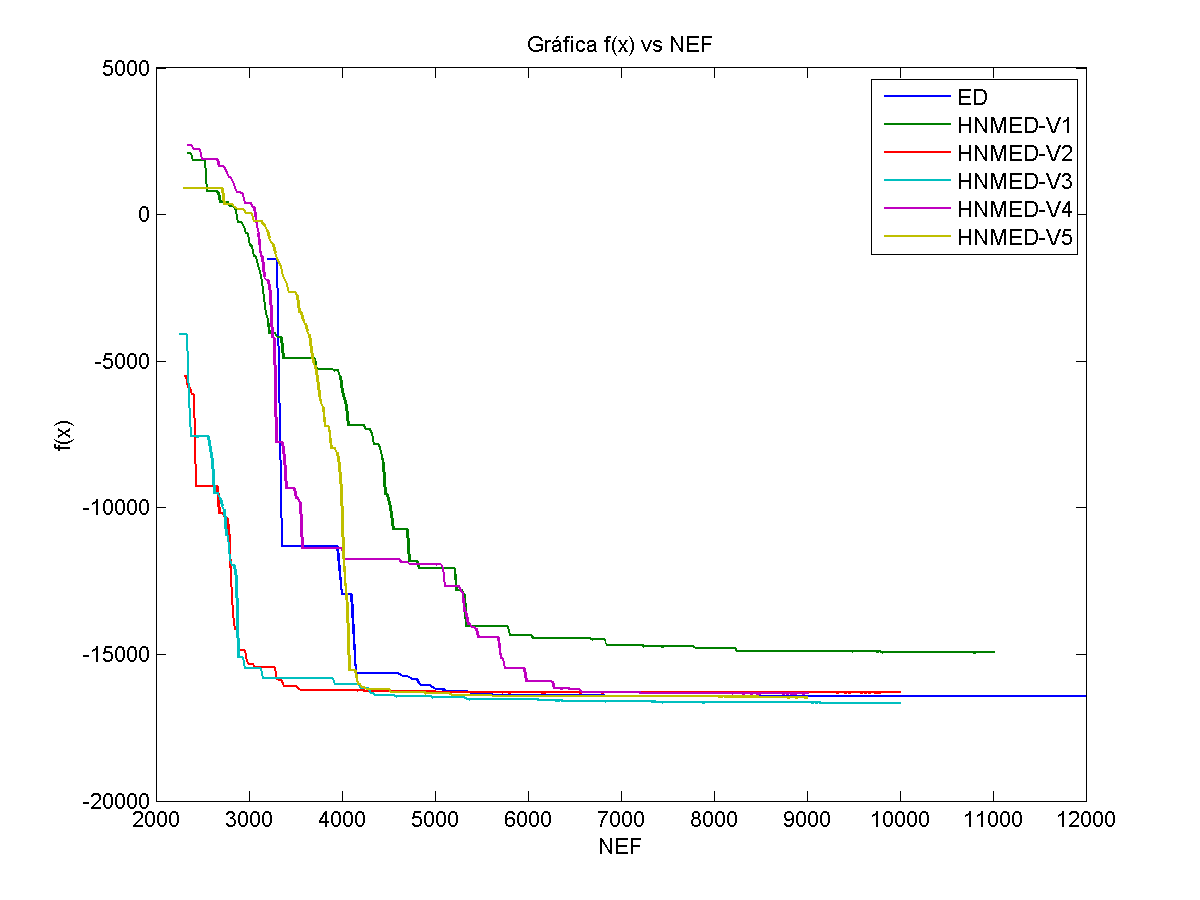
\includegraphics[width=\linewidth]{Figures/C-Grafica_Convergencia_Problema_6}
		\caption{SCE2} \label{fig:S1} 
	\end{subfigure}
	\caption{Gráficas de convergencia obtenidas por las variantes HNMED y ED/rand/1/bin en el Experimento C} \label{fig: Gráficas de convergencia para las variantes HNMED y ED/rand/1/bin para el Experimento C} 
	
\end{figure}
\begin{table}
	\centering
	\caption{Resultados de la prueba de Friedman en las variantes HNMED y DE/rand/1/bin en el experimento C para los seis problemas de diseño mecatrónico.}
	\label{tab:Resultados de la prueba de Friedman en las variantes HNMED y DE/rand/1/bin en el experimento C para los seis problemas de diseño mecatrónico.}
	\resizebox{\textwidth}{!}{%{0.3132\textheight}{%
		\begin{tabular}{lccccc}
			\hline
			Problema              & Algoritmo     & Jerarquía promedio &Valor de $p$        & $H_0$                           & $H_1$             \\
			\hline  
			\multirow{6}{*}{MCE1} & HNMED-V1      &3.6451E+00          &\multirow{6}{*}{1.1011E-02}  & \multirow{6}{*}{Rechazada}& \multirow{6}{*}{Aceptada} \\
			& HNMED-V2      & 3.3870E+00        &                    &                          &                            \\
			& HNMED-V3      &  4.0000E+00       &                    &                          &                            \\
			& HNMED-V4      &  3.9677E+00        &                    &                          &                            \\
			& HNMED-V5      &  3.5806E+00        &                    &                          &                            \\
			& ED/rand/1/bin &\textbf{2.4193E+00} &                    &                          &                            \\
			
			\hline  
			\multirow{6}{*}{MCE2} & HNMED-V1      & 3.7096E+00         & \multirow{6}{*}{2.1026E-12} & \multirow{6}{*}{Rechazada}& \multirow{6}{*}{Aceptada} \\
			& HNMED-V2      &3.0322E+00&                    &                          &                            \\
			& HNMED-V3      & 2.74193E+00         &                    &                          &                            \\
			& HNMED-V4      & 2.9032E+00         &                    &                          &                            \\
			& HNMED-V5      &\textbf{2.7741E+00 }&                    &                          &                            \\
			& ED/rand/1/bin &   5.8387E+00       &                    &                          &                            \\
			\hline
			
			\multirow{6}{*}{MCE3} & HNMED-V1      &  3.580645        & \multirow{6}{*}{4.4788E-03}  & \multirow{6}{*}{Rechazada}& \multirow{6}{*}{Aceptada} \\
			& HNMED-V2      & 4.0000E+00        &                    &                          &                            \\
			& HNMED-V3      & 3.9193E+00         &                    &                          &                            \\
			& HNMED-V4      & 3.5806E+00         &                    &                          &                            \\
			& HNMED-V5      &  3.6290E+00         &                    &                          &                            \\
			& ED/rand/1/bin & \textbf{2.2903E+00}    &                    &                          &                            \\
			
			
			
			\hline  
			\multirow{6}{*}{GCE1} & HNMED-V1      &   4.6451E+00       & \multirow{6}{*}{1.3274E-20}  & \multirow{6}{*}{Rechazada}& \multirow{6}{*}{Aceptada} \\
			& HNMED-V2      &   2.500E+00       &                    &                          &                            \\
			& HNMED-V3      &   2.6290E+00       &                    &                          &                            \\
			& HNMED-V4      &   3.4354E+00       &                    &                          &                            \\
			& HNMED-V5      &\textbf{1.8870E+00} &                    &                          &                            \\
			& ED/rand/1/bin &   5.9032E+00       &                    &                          &                            \\
			\hline  
			
			\multirow{6}{*}{GCE2} & HNMED-V1      &  4.5483E+00        & \multirow{6}{*}{3.9377E-03}  & \multirow{6}{*}{Rechazada}& \multirow{6}{*}{Aceptada} \\
			& HNMED-V2      &  3.8709E+00        &                    &                          &                            \\
			& HNMED-V3      & \textbf{ 3.0322E+00}                    &                          &                          &  \\
			& HNMED-V4      &  3.2580E+00         &                    &                          &                            \\
			& HNMED-V5      & 3.7741E+00          &                    &                          &                            \\
			& ED/rand/1/bin & 2.5161E+00&        &                     &                            \\
			\hline 
			
			\multirow{6}{*}{SCE1} & HNMED-V1      & 3.1935E+00                   & \multirow{6}{*}{ 3.2643E-02 }  & \multirow{6}{*}{Rechazada}& \multirow{6}{*}{Aceptada} \\
			& HNMED-V2      & 4.3225E+00                   &                    &                          &                            \\
			& HNMED-V3      & 3.3870E+00                   &                    &                          &                            \\
			& HNMED-V4      & 3.9032E+00                   &                    &                          &                            \\
			& HNMED-V5      & \textbf{2.8709E+00 }         &                    &                          &                            \\
			& ED/rand/1/bin &3.3225E+00 &                  &                    &                            \\
			
		\end{tabular}
	}
\end{table}



% Pruebas de Bunferroni

\begin{figure}
	\centering
	\begin{subfigure}[b]{0.49\linewidth}
		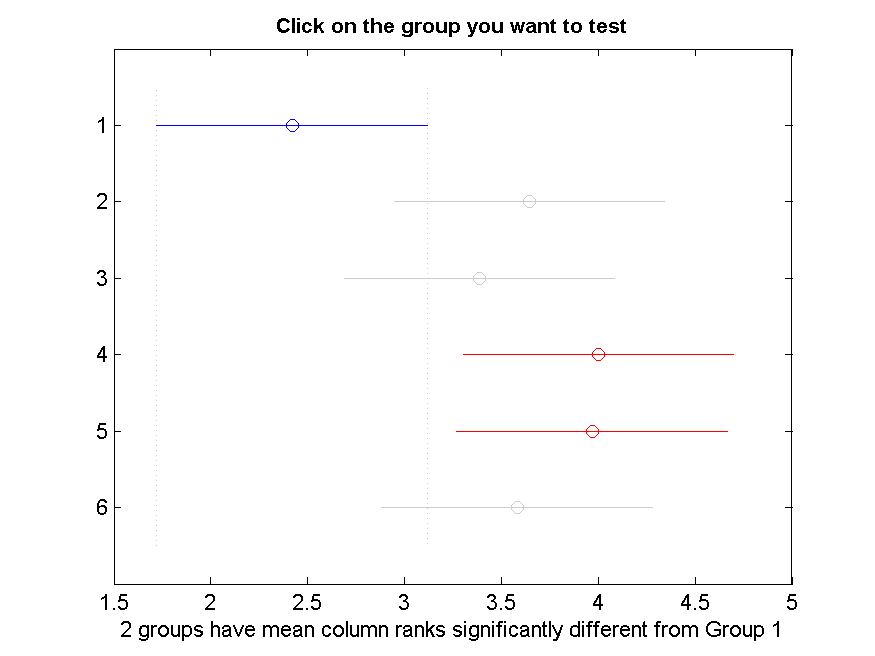
\includegraphics[width=\linewidth]{Figures/D-Bonferroni_HNMED_VS_ED1}
		\caption{MCE1} \label{fig:Bon_M1} 
	\end{subfigure}
	\begin{subfigure}[b]{0.49\linewidth}
		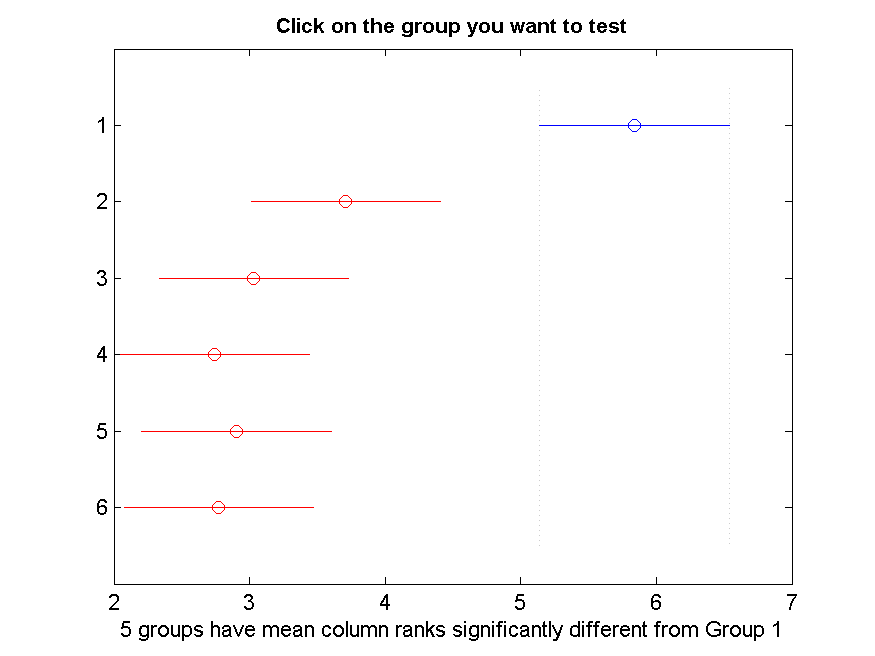
\includegraphics[width=\textwidth]{Figures/D-Bonferroni_HNMED_VS_ED2}
		\caption{MCE2} \label{fig:Bon_M2} 
	\end{subfigure}
	\begin{subfigure}[b]{0.49\linewidth}
		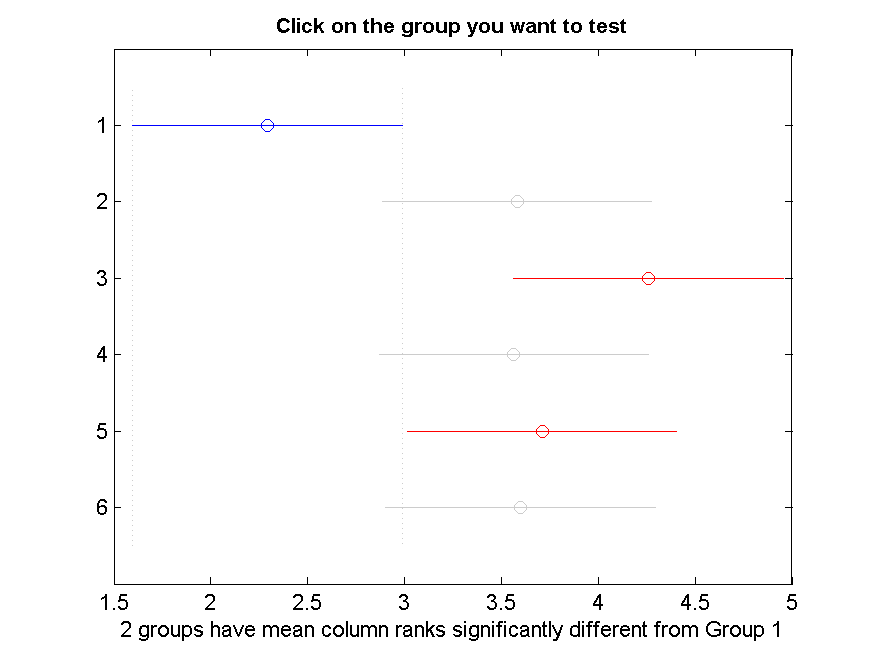
\includegraphics[width=\linewidth]{Figures/D-Bonferroni_HNMED_VS_ED3}
		\caption{MCE3} \label{fig:Bon_M3} 
	\end{subfigure}
	\begin{subfigure}[b]{0.49\linewidth}
		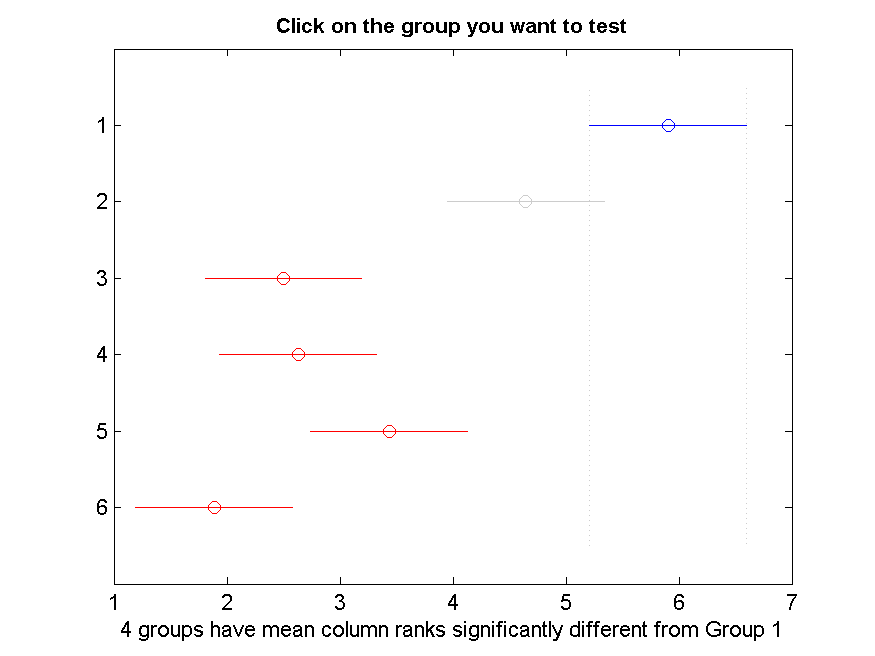
\includegraphics[width=\linewidth]{Figures/D-Bonferroni_HNMED_VS_ED4}
		\caption{GCE1} \label{fig:Bon_G1} 
	\end{subfigure}
	\begin{subfigure}[b]{0.49\linewidth}
		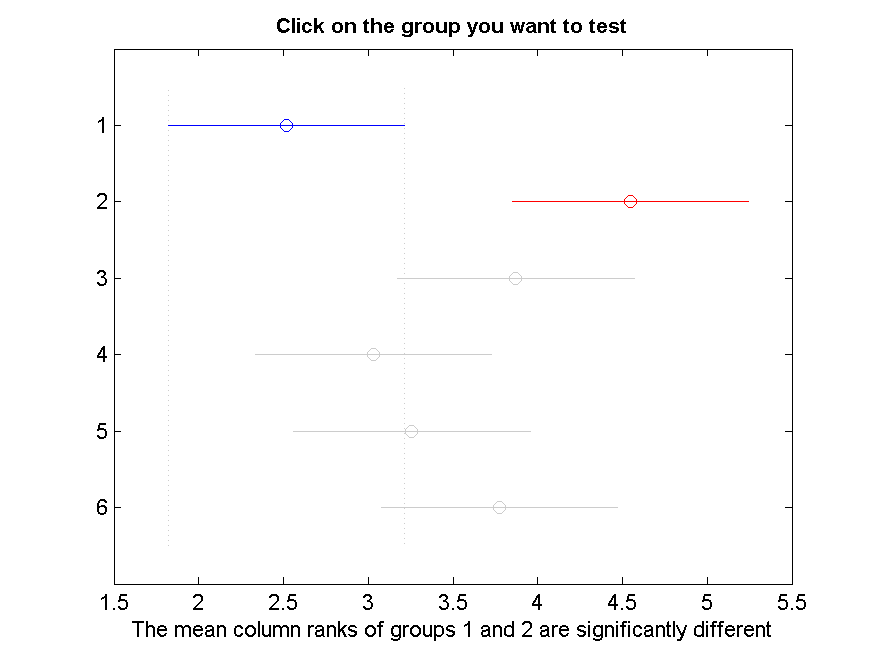
\includegraphics[width=\linewidth]{Figures/D-Bonferroni_HNMED_VS_ED5}
		\caption{GCE2} \label{fig:Bon_G2} 
	\end{subfigure}
	\begin{subfigure}[b]{0.49\linewidth}
		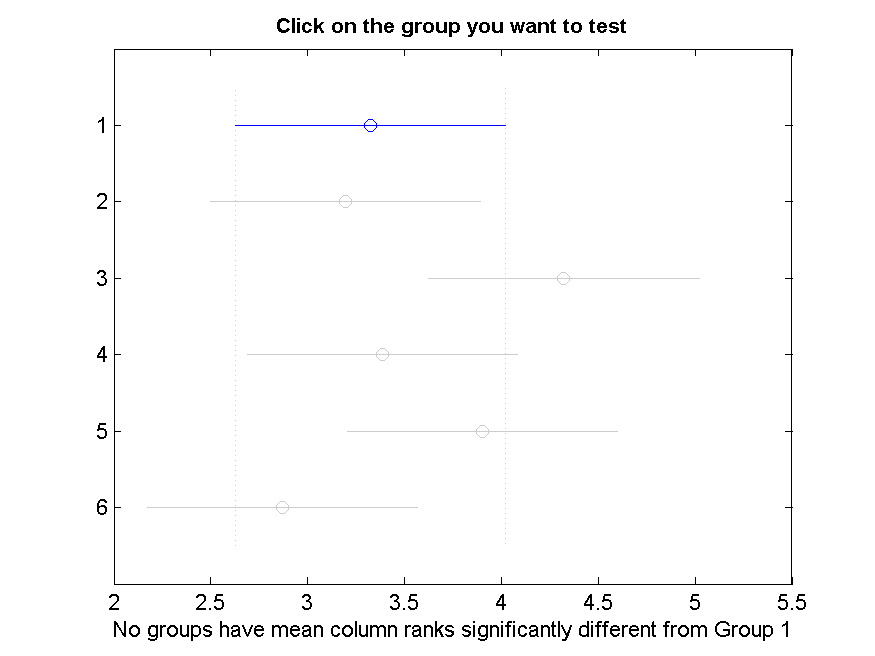
\includegraphics[width=\linewidth]{Figures/D-Bonferroni_HNMED_VS_ED6}
		\caption{SCE1} \label{fig:Bon_S1} 
	\end{subfigure}
	\caption{Resultados de las pruebas de Bonferroni-Dunn para las variantes HNMED vs ED/rand/1/bin en el experimento C.} \label{fig: Resultados de las pruebas de Bonferroni-Dunn para las variantes HNMED vs ED/rand/1/bin en el experimento C.} 
	
\end{figure}
\subsubsection{Observaciones}
Teniendo en cuenta los resultados obtenidos en ambos experimentos se pueden realizar las siguientes observaciones:
\begin{enumerate}
	\item Las variantes HNMED son capaces de encontrar resultados iguales o mejores para la mayoría de los problemas de optimización utilizando un número de evaluaciones menor, el cual representa un ahorro de más del 44\% en la mayoría de los problemas con excepción de MCE2 (-33.3\%) y SCE1 (-25.3\% para las variante HNMED-V4 y V5).      
	\item De forma similar a los resultados obtenidos en el experimento A, las curvas que describen funciones de convergencia obtenidas por las versiones de HNMED correspondientes a la mediana de las muestras se encuentran por debajo de la curva de la ED/ran/1/bin para la todos los problemas. Esto se logra reduciendo el número de símpleces y por tanto el tamaño de la población, esto implica un ahorro de evaluaciones por iteración y  permite realizar más operaciones de explotación. El hecho de que se alcancen los mínimos conocidos y valores de tendencia central competitivos descarta la posibilidad de HNMED presente convergencia prematura o estancamiento para los problemas presentados. 
	\item Al reducir el número de evaluaciones algunas versiones comienzan a presentar un desempeño significativamente inferior a la ED como es el caso de la V1. La variante HNMED-V5 es la que presenta mejor promedio de jerarquía en la mayoría de los problemas obteniendo resultados significativamente iguales o mejores que la ED.
\end{enumerate}



%%%%%%%%%%%%%%%%%%%%%%%%%%%%%%%%%%%%%%%%%%%%%%%%%%%%%%%%%%%%%%%%%%%%%%%%%%%%%%%%%%%%%%%%%%%%%%%%%%%%%%%%%%%%%%%%%%%%

\section{Experimentos finales}
Los experimentos iniciales permitieron observar el comportamiento de las variantes HNMED diseñadas bajo el enfoque de hibridación propuesto en la sección \ref{sec:Enfoque propuesto}. Se evidenció que a pesar de la rapidez de estos algoritmos, se presentaron dificultades en los problemas MCE1, MCE3 y GCE2. Estos problemas presentan un espacio de búsqueda más complejo, ya sea por presentar mayor número de restricciones, dimesionalidad, complejidad de la función objetivo o la cualquier combinación de estas características. Las variantes propuestas heredan, en cierta medida, algunas deficiencias del método de búsqueda local utilizado como la reducción del desempeño ante un aumento de la dimesionalidad del problema y la sensibilidad a los puntos iniciales. Por tanto, una mayor capacidad de exploración es requerida en orden de alcanzar mejores resultados. Con este objetivo trazado se diseño la HNMED-V6 cuyo desempeño es medido en los experimentos finales junto a la variante HNMED-V5.


\subsection{Experimentos D y E : Comparación de Variantes HNMED-V5 y HNMED-V6 con Algoritmo C-LSHADE}
El objetivo de ambos experimentos es comprobar la competitividad  de las dos mejores versiones HNMED. Por tanto, se realizan dos comparaciones finales por medio de estadística descriptiva e inferencial: el algoritmo HNMED-V5 y HNMED-V6 con el algoritmo C-LSHADE propuesto por Zapata en \cite{zapata_zapata_control_2017}.
\subsubsection{Definición de medidas}
Se obtiene para cada algoritmo una muestra de $n=31$ ejecuciones. Para cada problema las observaciones en la muestra corresponden al valor de la función objetivo del mejor individuo factible encontrado por el algoritmo $A_i$en la ejecución $j$ para $j= \{ 1,2,...,n\}$. Se aplicarán al conjunto de muestras las siguientes pruebas de estadística descriptiva e inferencial:
\begin{enumerate}
	\item \textbf{Estadística descriptiva}: Se obtiene la la mejor y peor solución, mediana, promedio y desviación estándar de las muestras
	\item \textbf{Tasa de convergencia}: Se presenta la gráfica de convergencia correspondiente a la mediana de la muestra para cada los dos algoritmo en comparación.
	\item \textbf{Prueba suma de Jerarquías de Wilcoxon}: con nivel significancia $\alpha=0.05$ para determinar si existen diferencias significativas entre el desempeño los dos algoritmos comparados. 
	
\end{enumerate}
\subsubsection{Planificación pre-experimental y configuración}
Para este experimento se mantuvo el número de evaluaciones realizadas por C-LSHADE según se describe en \cite{zapata_zapata_control_2017}. En la Tabla \ref{tab:Evaluaciones utilizadas por problema de optimización: Experimentos D y E.} se describe el número de evaluaciones realizadas por cada algoritmo comparado.

\begin{table}[]
	
	\caption{Evaluaciones utilizadas por problema de optimización: Experimentos D y E.}
	\label{tab:Evaluaciones utilizadas por problema de optimización: Experimentos D y E.}
	\centering
	
	\begin{tabular}{ccccccc}
		\textbf{Problema} &   C-LCHADE     &HNMED-V5&HNMED-V6 \\
		\hline
		MCE1   &   400000 &400000 &350000   \\
		MCE2   &   15000  &15000  &10000   \\
		MCE3   &   200000 &25000  &175000  \\
		GCE1   &   325000 &125000  &100000\\
		GCE2   &   150000 &225000  &125000\\
		SCE1   &   240000 &210000  &210000\\
	\end{tabular}
	
\end{table}
La configuración de parámetros utilizada por las variantes HNMED-V6:
\begin{enumerate}
	\item Se establece la probabilidad de cruza $CR=\{0.8, 1\}$ para ED y HNMED para todos los problemas.
	\item Se establece el factor de escala $F=\{0.3, 0.9\}$ para ED y HNMED para todos los problemas.
	\item Se establecieron los parámetros de reflexión $\alpha=2$, expansión $\gamma=1.7$ $\beta=0.3$ para todos los problemas.
	\item El tamaño de población utilizado se ajusta para cada algoritmo según la Tabla \ref{tab:Tamaños de población utilizados para cada problema en los experimentos finales}. 
\end{enumerate}

\begin{table}[]
	\centering
	\caption{Tamaños de población utilizados para cada problema en los experimentos finales}
	\label{tab:Tamaños de población utilizados para cada problema en los experimentos finales}
	
	\begin{tabular}{cccccccccccc}
		& \textbf{C-LSHADE } & \multicolumn{2}{l}{\textbf{HNMED-V5}}&\multicolumn{2}{l}{\textbf{HNMED-V6}}\\
		\hline
		\textbf{Problema} & \textbf{NP}    & \textbf{NS} & \textbf{NP}& \textbf{NS}& \textbf{NP}\\
		\hline
		MCE1     & 138           & 9           & 144 &8&128   \\
		MCE2     & 50            & 3           & 21  &4&28       \\
		MCE3     & 138           & 7           & 140 &5&75      \\
		GCE1     & 138           & 9           & 135 &7&105        \\
		GCE2     & 138           & 9           & 135 &7&105    \\
		SCE1     & 50            & 7           & 35  &2&10       
	\end{tabular}
	
\end{table}


\subsubsection{Resultados del Experimento D}
La Tabla \ref{tab:Resultados estadísticos obtenidos por HNMED-V5 y el algoritmo C-LSHADE en los seis problemas de diseño mecatrónico} se muestran los resultados estadísticos obtenidos por HNMED-V5 y los obtenidos por C-LSHADE en \cite{zapata_zapata_control_2017}. En la Figura \ref{fig: Gráficas de convergencia obtenidas por HNMED-V5 y CLSHADE para el Experimento D} se presentan las gráficas de convergencias correspondientes al Expermiento D para los seis problemas. Finalmente, la Tabla \ref{tab:Wilcoxon HNMED-V5-CLSHADE} contiene los resultados de la prueba de suma de jerarquías de Wilcoxon con un nivel de significancia de 95\%.
%%%%%%%%%%%%%%%%%%%%%%%%%%%%%%%%%%%%%%%%%%%%%%%%%%%%%%%%%%%%%%%%%%%%%%%%%%%%%%%%%%%%%%%%%%%%%%%%%%%

\begin{table}
	\centering
	\caption[Resultados estadísticos obtenidos por HNMED-V5 y el algoritmo C-LSHADE
	en los seis problemas de diseño mecatrónico en el Experimento D]{Resultados estadísticos obtenidos por HNMED-V5 y el algoritmo C-LSHADE
		en los seis problemas de diseño mecatrónico en el Experimento D. Se marcan en negritas los
		mejores valores de cada medida.}\label{tab:Resultados estadísticos obtenidos por HNMED-V5 y el algoritmo C-LSHADE en los seis problemas de diseño mecatrónico}
	\begin{tabular}{clcc} 
		\hline
		Problema              & Estadística   & HNMED-V5 & C-LSHADE  \\ 
		\hline
		\multirow{6}{*}{MCE1} & Mejor        & 6.3108E-29 & \textbf{0 }      \\
		& Peor         &2.7323E-02&  \textbf{6.4277E-04}  \\
		& Mediana      &3.2843E-04&\textbf{3.6143E-08}     \\
		& Promedio     &2.5730E-03& \textbf{ 2.4021E-04 } \\
		& Desv. Est.   &6.9657E-03&\textbf{ 2.7680E-04}\\
		& Evaluaciones &400000   &  400000       \\
		\hline
		\multirow{6}{*}{MCE2} & Mejor        &2.6280E-03&2.6280E-03
		\\
		& Peor         &\textbf{2.6280E-03}&2.6281E-03                \\
		& Mediana      &2.6280E-03&2.6280E-03   \\
		& Promedio     &2.6280E-03&2.6280E-03    \\
		& Desv. Est.   &\textbf{2.1708E-10}&8.5532E-09 \\
		& Evaluaciones &15000&15000                \\
		\hline
		\multirow{6}{*}{MCE3} & Mejor        &2.7577E-01&\textbf{2.7496E-01}  \\
		& Peor         &1.3508E+01&1.3508E+01     \\
		& Mediana      &5.0946E-01&\textbf{2.8886E-01} \\
		& Promedio     &4.8813E+00&\textbf{1.6068E+00}\\
		& Desv. Est.   &6.2202E+00&\textbf{3.9629E+00}\\
		& Evaluaciones &225000& \textbf{200000} (-12.5\%) \\
		\hline
		\multirow{6}{*}{GCE1} & Mejor        &0&0\\
		& Peor         &7.6992E-28&\textbf{3.0292E-28}\\
		& Mediana      &1.8932E-29&\textbf{1.2621E-29}\\
		& Promedio     &1.0886E-28&\textbf{2.7991E-28} \\
		& Desv. Est.   &1.7494E-28&\textbf{5.6901E-29}\\
		& Evaluaciones &\textbf{125000}(-61.5\%)&325000 \\
		\hline
		\multirow{6}{*}{GCE2} & Mejor        &1.1385E-01&1.1385E-01\\
		& Peor         &1.6276E-01&\textbf{1.5783E-01}\\
		& Mediana      &1.1631E-01&\textbf{1.1392E-01 }\\
		& Promedio     &1.2887E-01&\textbf{1.2066E-01  }\\
		& Desv. Est.   &1.9809E-02&\textbf{1.5457E-02 }\\
		& Evaluaciones &250000&\textbf{150000}(-40.0\%) \\
		\hline
		
		
		\multirow{6}{*}{SCE1} & Mejor        &\textbf{-5.3652E+05}&-5.3205E+05 \\
		& Peor         &-5.3080E+05&-5.3205E+05\\
		& Mediana      &\textbf{-5.3217E+05}&-5.3205E+05\\
		& Promedio     &\textbf{5.3230E+05}&-5.3205E+05\\
		& Desv. Est.   &1.094E+03&\textbf{1.0515E-04}\\
		& Evaluaciones &\textbf{216000}(-10.0\%)&240000 \\
		
		
		\hline
	\end{tabular}
\end{table}


\begin{figure}
	\centering
	\begin{subfigure}[b]{0.49\linewidth}
		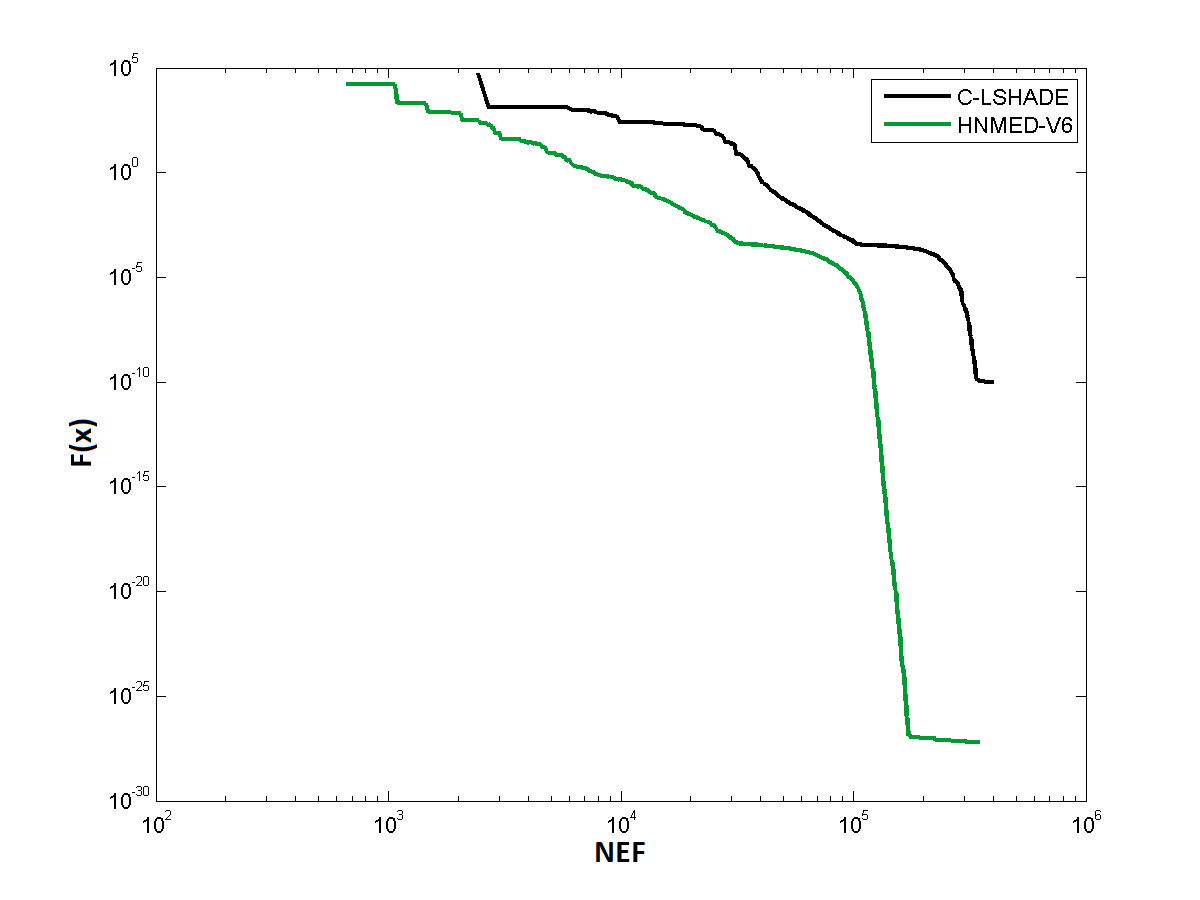
\includegraphics[width=\linewidth]{Figures/E-Grafica_Convergencia_Problema_1}
		\caption{MCE1} \label{fig:M1} 
	\end{subfigure}
	\begin{subfigure}[b]{0.49\linewidth}
		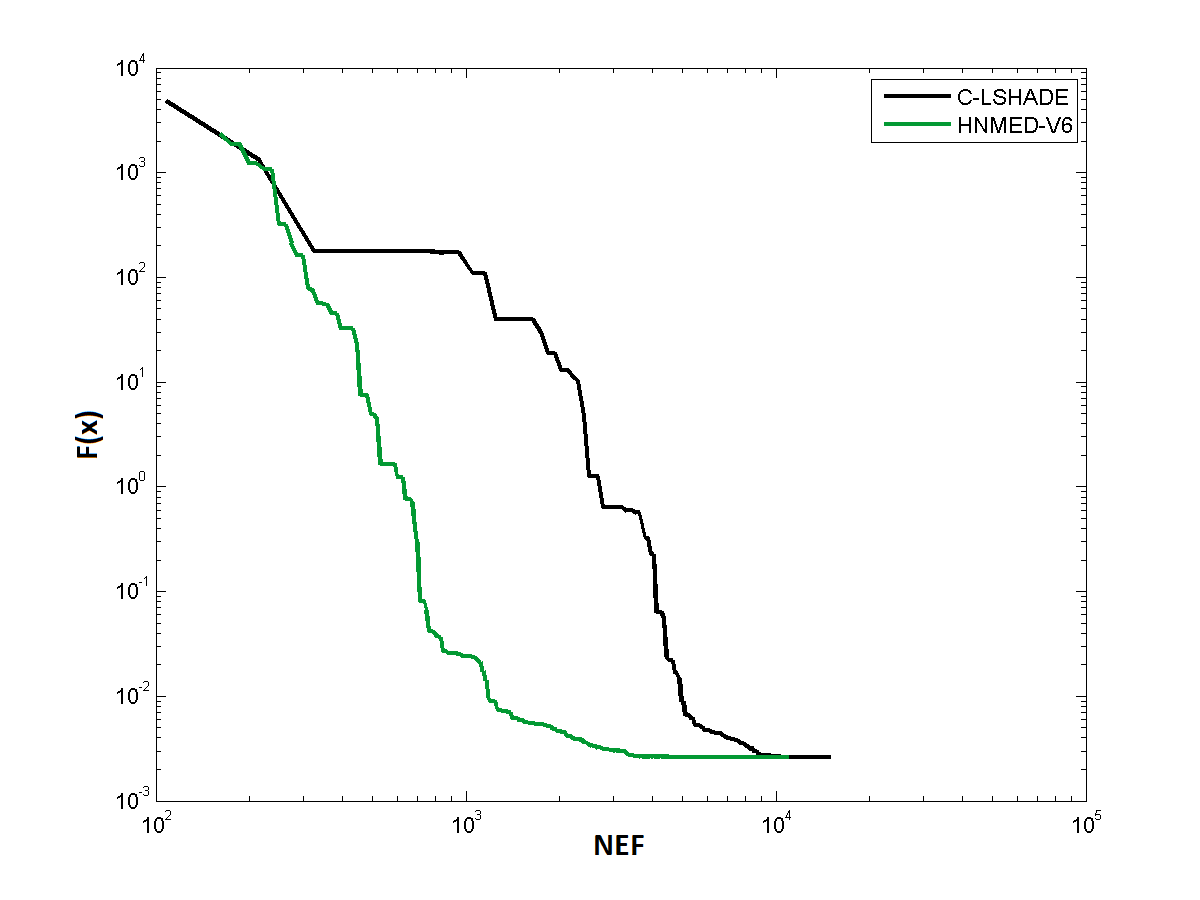
\includegraphics[width=\textwidth]{Figures/E-Grafica_Convergencia_Problema_2}
		\caption{MCE2} \label{fig:M2} 
	\end{subfigure}
	\begin{subfigure}[b]{0.49\linewidth}
		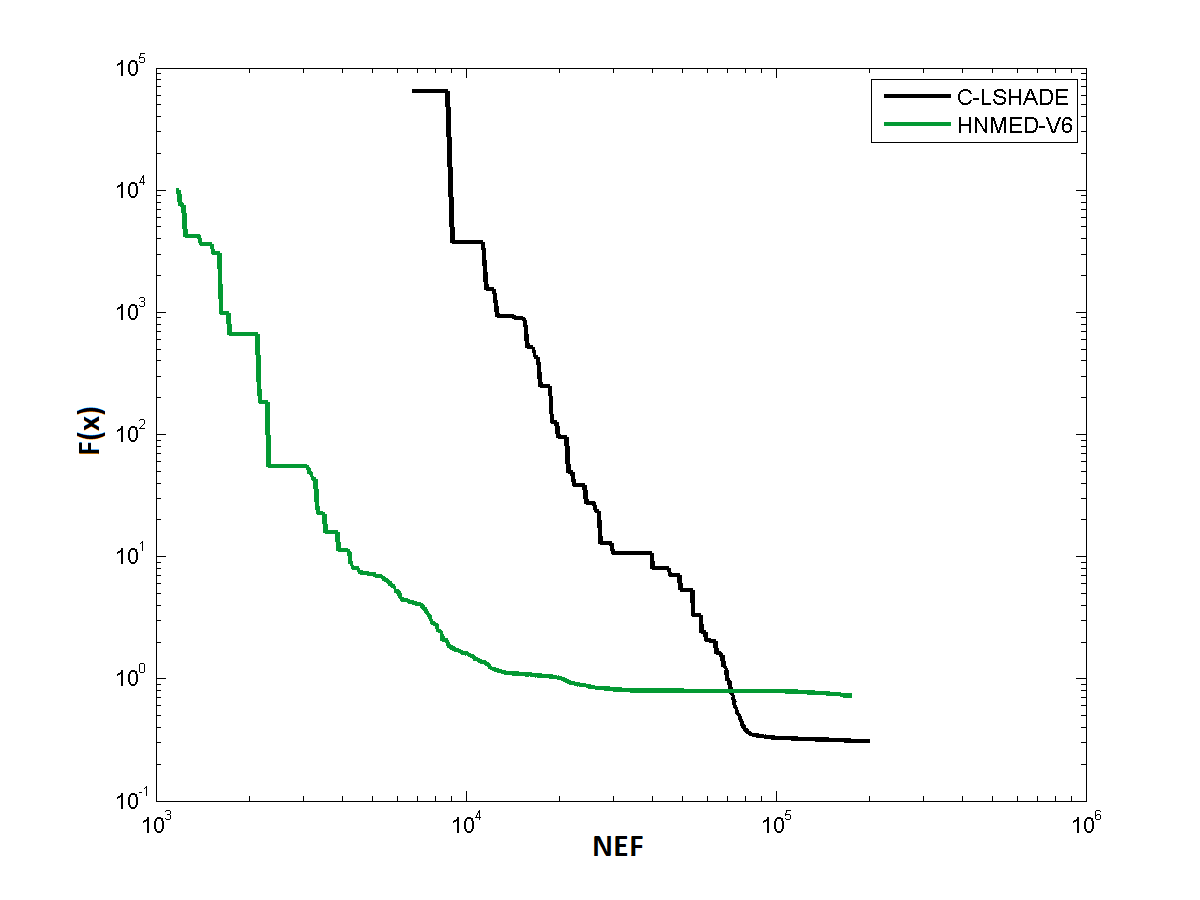
\includegraphics[width=\linewidth]{Figures/E-Grafica_Convergencia_Problema_3}
		\caption{MCE3} \label{fig:M3} 
	\end{subfigure}
	\begin{subfigure}[b]{0.49\linewidth}
		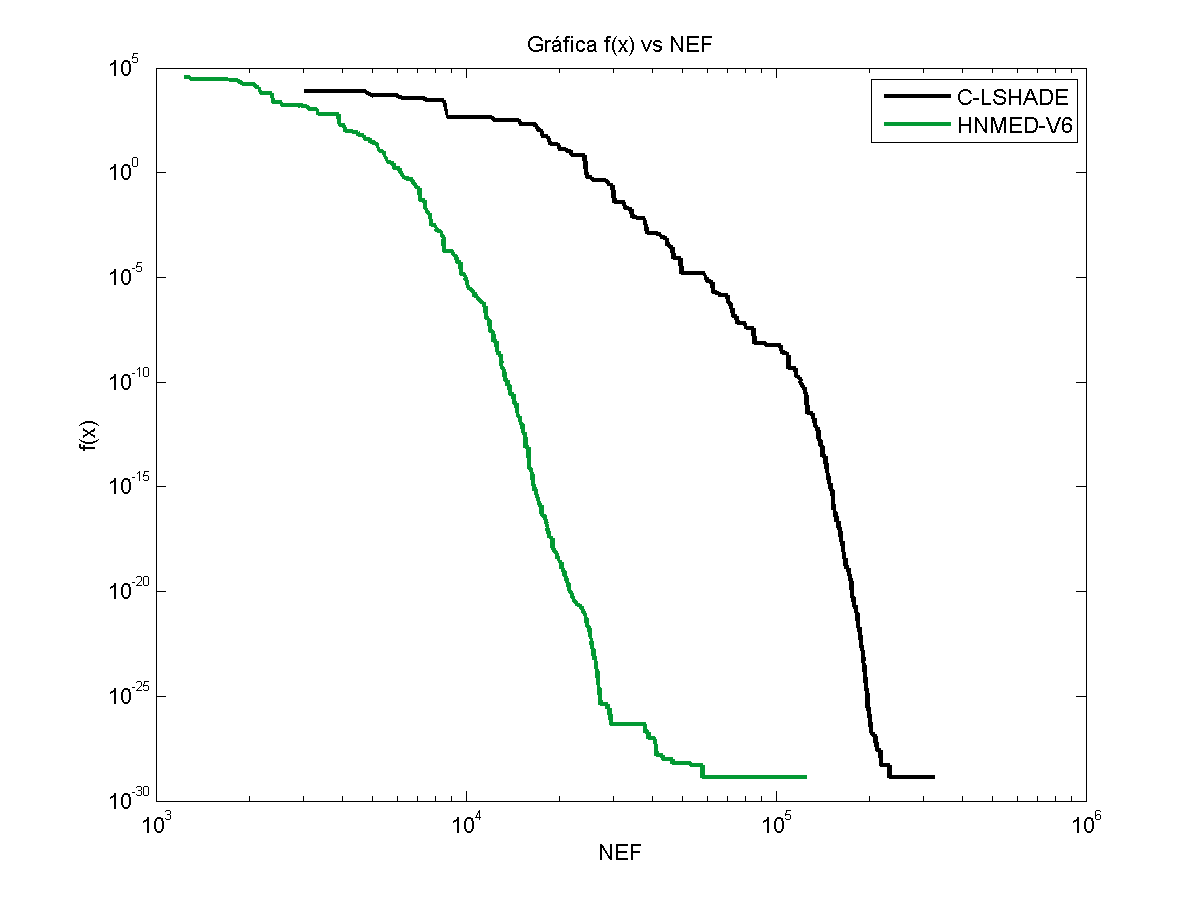
\includegraphics[width=\linewidth]{Figures/E-Grafica_Convergencia_Problema_4}
		\caption{GCE1} \label{fig:G1} 
	\end{subfigure}
	\begin{subfigure}[b]{0.49\linewidth}
		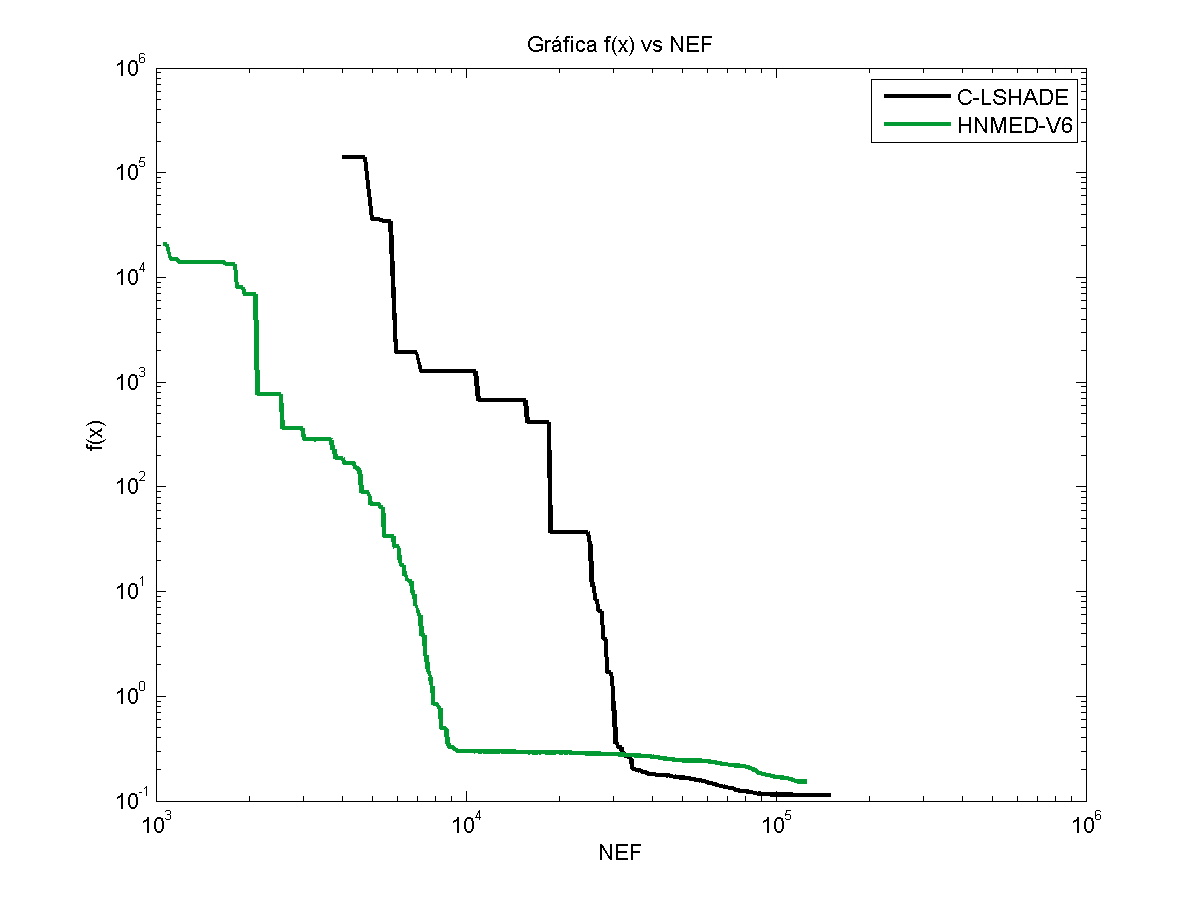
\includegraphics[width=\linewidth]{Figures/E-Grafica_Convergencia_Problema_5}
		\caption{GCE2} \label{fig:G2} 
	\end{subfigure}
	\begin{subfigure}[b]{0.49\linewidth}
		\includegraphics[width=\linewidth]{Figures/E-Grafica_Convergencia_Problema_6}
		\caption{SCE2} \label{fig:S1} 
	\end{subfigure}
	\caption{Gráficas de convergencia obtenidas por HNMED-V5 y CLSHADE para el Experimento D.} \label{fig: Gráficas de convergencia obtenidas por HNMED-V5 y CLSHADE para el Experimento D} 
	
\end{figure}

\begin{table}
	\centering
	\caption[Comparación de C-LSHADE y HNMED-V5 en los seis problemas de optimización mediante la prueba de Suma de jerarquías de Wilcoxon]{Comparación de C-LSHADE y HNMED-V5 en los seis problemas de optimización. Los símbolos +, - y $\approx$ señalan que HNMED-V5 obtuvo un desempeño significativamente mejor (+), significativamente peor (-) o no significativamente diferente ($\approx$) comparado contra C-LSHADE usando la prueba de suma de jerarquías de Wilcoxon con un 95 \% de confianza} \label{tab:Wilcoxon HNMED-V5-CLSHADE}
	\begin{tabular}{cccccccc}
		\multirow{2}{*}{\textbf{vs C-LSHADE}} & \multicolumn{6}{c}{\textbf{Problemas}}           & \textbf{Total}  \\
		& MCE1 & MCE2 & MCE3 & GCE1 & GCE2 & SCE1 &        \\
		\hline
		\multirow{3}{*}{HNMED-V5}    &      &  $+$    &      &      &       & $ +$    &  2      \\
		&   $-$  &      &  $ -$   &      &  $ - $  &       & 3       \\
		&      &      &       &$\approx$ &  &        &    1
	\end{tabular}
\end{table}
%%%%%%%%%%%%%%%%%%%%%%%%%%%%%%%%%%%%%%%%%%%%%%%%%%%%%%%%%%%%%%%%%%%%%%%%%%%%%%%%%%%%%%%%%%%%%%%%%%%


\subsubsection{Resultados del Experimento E}
Las Tablas \ref{tab:Resultados estadísticos obtenidos por variantes HNMED6 y ED  en experimento E.} y \ref{tab:Resultados estadísticos obtenidos por variantes HNMED6 y CLSHADE  en experimento E.} se muestran los resultados estadísticos obtenidos por la HNMED-V6 frente a la ED/rand/1/bin y C-LSHADE respectivamente. Se agrega la comparación estadística de HNMED-V6 con la ED/rand/1/bin para evidenciar la reducción del número evaluaciones. En la Figura \ref{fig: Gráficas de convergencia obtenidas por HNMED-V6 y CLSHADE para el Experimento E.} se muestran las gráficas de convergencia correspondientes al Experimento E. En la Tabla \ref{tab:Wilcoxon HNMED-V6-CLSHADE} se presenta para la comparación de HNMED-V6 y C-LSHADE mediante prueba de suma de jerarquías de Wilcoxon.  

\begin{table}
	\centering
	\caption[Resultados estadísticos obtenidos por HNMED-V6 vs ED/rand/1/bin
	en los seis problemas de diseño mecatrónico.]{Resultados estadísticos obtenidos por HNMED-V6 vs ED/rand/1/bin
		en los seis problemas de diseño mecatrónico en el experimento E. Se marcan en negritas los
		mejores valores de cada medida.} \label{tab:Resultados estadísticos obtenidos por variantes HNMED6 y ED  en experimento E.}
	\begin{tabular}{clcc} 
		\hline
		Problema              & Estadística  & HNMED-V5 & ED/rand/1/bin  \\ 
		\hline
		\multirow{6}{*}{MCE1} & Mejor        & \textbf{3.7865E-29} &1.7670E-28          \\
		& Peor         &\textbf{3.6342E-03}&2.7649E-02
		\\
		& Mediana      &\textbf{6.5633E-28}&4.2746E-06            \\
		& Promedio     &\textbf{1.6110E-04}&2.9850E-01            \\
		& Desv. Est.   &\textbf{6.4886E-04}& 8.1906E-03
		\\
		& Evaluaciones &\textbf{350000}(-53.53\%)  &  750030       \\
		\hline
		
		\multirow{6}{*}{MCE2} & Mejor        &\textbf{2.5643E-04}&2.6280E-03
		\\
		& Peor         &\textbf{2.6280E-03}&2.6426E-03  \\
		& Mediana      &2.6280E-03&2.6280E-03   \\
		& Promedio     &\textbf{2.3985E-03}&2.6288E-03   \\
		& Desv. Est.   &7.1276E-04&\textbf{2.7205E-06} \\
		& Evaluaciones &\textbf{10000}(50.0\%) &20000                \\
		\hline
		
		\multirow{6}{*}{MCE3} & Mejor        &2.7496E-01&2.7496E-01  \\
		& Peor         &1.3508E+01&1.3508E+01     \\
		& Mediana      &3.0867E-01&\textbf{2.7563E-01} \\
		& Promedio     &2.4412E+00&\textbf{1.2313E+00}\\
		& Desv. Est.   &4.7466E+00&\textbf{3.2919E+00}\\
		& Evaluaciones &\textbf{175000}(-61.1\%)& 450018 \\
		\hline
		\multirow{6}{*}{GCE1} & Mejor        &\textbf{0}&6.7147E-27\\
		& Peor         &\textbf{5.3327E-28}&5.9926E-20\\
		& Mediana      &\textbf{1.2621E-29}&3.9485E-23\\
		& Promedio     &\textbf{5.8223E-29}&3.4957E-21\\
		& Desv. Est.   &\textbf{1.1714E-28}&1.2077E-20\\
		& Evaluaciones &\textbf{100000}(-86.6\%)&750030 \\
		\hline
		
		
		\multirow{6}{*}{GCE2} & Mejor        &1.1385E-01&1.1385E-01\\
		& Peor         &2.3331E-01&\textbf{1.6075E-01}\\
		& Mediana      &1.5210E-01&\textbf{1.1447E-01 }\\
		& Promedio     &1.4351E-01&\textbf{1.2080E-01  }\\
		& Desv. Est.   &3.3531E-02&\textbf{1.4713E-02 }\\
		& Evaluaciones &\textbf{125000}(-72.2\%)&450018 \\
		\hline
		\multirow{6}{*}{SCE1} & Mejor        &\textbf{ -5.5147E+05}&-5.3206E+05 \\
		& Peor         &\textbf{ -5.5147E+05}&-5.3204E+05\\
		& Mediana      &\textbf{ -5.5147E+05}&-5.3205E+05\\
		& Promedio     & \textbf{-5.5147E+05}&-5.3205E+05\\
		& Desv. Est.   &\textbf{2.3667E-10}&3.3010E+00\\
		& Evaluaciones &\textbf{216000}(-25.0\%)&288000 \\
		
		
		\hline
	\end{tabular}
\end{table}

\begin{table}
	\centering
	\caption[Resultados estadísticos obtenidos por HNMED-V6 vs C-LSHADE
	en los seis problemas de diseño mecatrónico]{Resultados estadísticos obtenidos por HNMED-V6 vs C-LSHADE
		en los seis problemas de diseño mecatrónico. Se marcan en negritas los
		mejores valores de cada medida.} \label{tab:Resultados estadísticos obtenidos por variantes HNMED6 y CLSHADE  en experimento E.}
	\begin{tabular}{clcc} 
		\hline
		Problema              & Estadística   & HNMED-V6 & C-LSHADE  \\ 
		\hline
		\multirow{6}{*}{MCE1} & Mejor        & 3.7865E-29 &\textbf{ 0 }            \\
		& Peor         &3.6342E-03&  \textbf{6.4277E-04}
		\\
		& Mediana      &\textbf{6.56332E-28}&3.6143E-08            \\
		& Promedio     &\textbf{1.6110E-04}&  2.4021E-04             \\
		& Desv. Est.   &6.4886E-04& \textbf{2.7680E-04 }         \\
		& Evaluaciones &\textbf{350000}(-12.5\%)  &  400000       \\
		\hline
		
		\multirow{6}{*}{MCE2} & Mejor        &\textbf{2.5643E-04}&2.6280E-03
		\\
		& Peor         &\textbf{2.6280E-03}&2.6281E-03                \\
		& Mediana      &2.6280E-03&2.6280E-03   \\
		& Promedio     &\textbf{2.3985E-03}&2.6280E-03    \\
		& Desv. Est.   &7.1276E-04&\textbf{8.5532E-09} \\
		& Evaluaciones &\textbf{10000}(30.0\%) &15000                \\
		\hline
		
		\multirow{6}{*}{MCE3} & Mejor        &2.7496E-01&2.7496E-01  \\
		& Peor         &1.3508E+01&1.3508E+01     \\
		& Mediana      &3.0867E-01&\textbf{2.8886E-01} \\
		& Promedio     &2.4412E+00&\textbf{1.6068E+00}\\
		& Desv. Est.   &4.7466E+00&\textbf{3.9629E+00}\\
		& Evaluaciones &\textbf{175000}(-22.2\%)& 200000 \\
		\hline
		\multirow{6}{*}{GCE1} & Mejor        &0&0\\
		& Peor         &5.3327E-28&\textbf{3.0292E-28}\\
		& Mediana      &1.2621E-29&1.2621E-29\\
		& Promedio     &\textbf{5.8223E-29}&2.7991E-28 \\
		& Desv. Est.   &1.1714E-28&\textbf{5.6901E-29}\\
		& Evaluaciones &\textbf{100000}(-61.5\%)&325000 \\
		\hline
		
		
		\multirow{6}{*}{GCE2} & Mejor        &1.1385E-01&1.1385E-01\\
		& Peor         &2.3331E-01&\textbf{1.5783E-01}\\
		& Mediana      &1.5210E-01&\textbf{1.1392E-01 }\\
		& Promedio     &1.4351E-01&\textbf{1.2066E-01  }\\
		& Desv. Est.   &3.3531E-02&\textbf{1.5457E-02 }\\
		& Evaluaciones &\textbf{125000}(-16.6\%)&150000 \\
		\hline
		\multirow{6}{*}{SCE1} & Mejor        &\textbf{ -5.5147E+05}&-5.3205E+05 \\
		& Peor         &\textbf{ -5.5147E+05}&-5.3205E+05\\
		& Mediana      &\textbf{ -5.5147E+05}&-5.3205E+05\\
		& Promedio     & \textbf{-5.5147E+05}&-5.3205E+05\\
		& Desv. Est.   &\textbf{2.3667E-10}&1.0515E-04\\
		& Evaluaciones &\textbf{216000}(-12.5\%)&240000 \\
		
		
		\hline
	\end{tabular}
\end{table}


\begin{figure}
	\centering
	\begin{subfigure}[b]{0.49\linewidth}
		\includegraphics[width=\linewidth]{Figures/F-Grafica_Convergencia_Problema_1}
		\caption{MCE1} \label{fig:M1} 
	\end{subfigure}
	\begin{subfigure}[b]{0.49\linewidth}
		\includegraphics[width=\textwidth]{Figures/F-Grafica_Convergencia_Problema_2}
		\caption{MCE2} \label{fig:M2} 
	\end{subfigure}
	\begin{subfigure}[b]{0.49\linewidth}
		\includegraphics[width=\linewidth]{Figures/F-Grafica_Convergencia_Problema_3}
		\caption{MCE3} \label{fig:M3} 
	\end{subfigure}
	\begin{subfigure}[b]{0.49\linewidth}
		\includegraphics[width=\linewidth]{Figures/F-Grafica_Convergencia_Problema_4}
		\caption{GCE1} \label{fig:G1} 
	\end{subfigure}
	\begin{subfigure}[b]{0.49\linewidth}
		\includegraphics[width=\linewidth]{Figures/F-Grafica_Convergencia_Problema_5}
		\caption{GCE2} \label{fig:G2} 
	\end{subfigure}
	\begin{subfigure}[b]{0.49\linewidth}
		\includegraphics[width=\linewidth]{Figures/F-Grafica_Convergencia_Problema_6}
		\caption{SCE2} \label{fig:S1} 
	\end{subfigure}
	\caption{Gráficas de convergencia obtenidas por HNMED-V6 y CLSHADE en el Experimento E.} \label{fig: Gráficas de convergencia obtenidas por HNMED-V6 y CLSHADE para el Experimento E.} 
	
\end{figure}


\begin{table}
	\centering
	\caption[Comparación de C-LSHADE y HNMED-V6 en los seis problemas de optimización mediante la prueba de Suma de jerarquías de Wilcoxon]{Comparación de C-LSHADE y HNMED-V6 en los seis problemas de optimización. Los símbolos +, - y $\approx$ señalan que HNMED-V6 obtuvo un desempeño significativamente mejor (+), significativamente peor (-) o no significativamente diferente ($\approx$) comparado contra LSHADE-CV usando la prueba de suma de jerarquías de Wilcoxon con un 95 \% de confianza} \label{tab:Wilcoxon HNMED-V6-CLSHADE}
	\begin{tabular}{cccccccc}
		\multirow{2}{*}{\textbf{vs C-LSHADE}} & \multicolumn{6}{c}{\textbf{Problemas}}           & \textbf{Total}  \\
	                                        	& MCE1 & MCE2 & MCE3 & GCE1 & GCE2 & SCE1 &        \\
		\hline
		\multirow{3}{*}{HNMED-V6}    &      &  $+$    &      &      &      &  $+$    &   2     \\
		&      &      & $-$     &      &    $-$  &      &    2    \\
		&$\approx$&   &         &$\approx$&      &       &  2     
	\end{tabular}
\end{table}

\subsubsection{Observaciones Finales}
Los resultados de los experimentos F y G permiten plantear las siguientes observaciones finales:
\begin{enumerate}
 \item La versión con peor desempeño en comparación a C-LSHADE resultó ser V5, la cual obtiene un desempeño significativamente inferior en los problemas MCE1, MCE3 y GCE2  y sólo alcanza mejores resultados para los problemas MCE2 y SCE1 (los de menor dimensión). A pesar de que HNMED-V5 es capaz de utilizar un número menor de evaluaciones para los problemas GCE1 y SCE1; para los casos MCE3 y GCE2 el algoritmo C-LSHADE utiliza menos evaluaciones de la función objetivo. Las gráficas de convergencia muestran que HNMED-V5 presenta mayor rapidez de convergencia respecto C-LSHADE, sin embargo el punto al que converge no siempre es mejor que el encontrado por C-LSHADE para todos los problemas de optimización.  

 \item  La versión más competitiva es HNMED-V6, lo que se evidencia tanto en las pruebas de estadística descriptiva como inferencial. HNMED-V6 obtienen resultados de mediana y promedio mejores que C-LSHADE en los problemas MCE1, MCE2, GCE1 y SCE1. Para el problema MCE2 se encuentra un nuevo mínimo $(f(\vec{x})=2.5643E-04)$ el cual supera al obtenido tanto por la ED/rand/1/bin como por C-LSHADE con valor de $(f(\vec{x})=2.6280E-03)$. En la sección de visualización de resultados se puede observar que éste mínimo se encuentra en un punto del espacio de búsqueda distante de la solución encontrada hasta el momento en la literatura. Para el problema de la micro-red aislada se logra encontrar un ahorro total significativamente mayor con un valor de $\sum_{1}^{24}f(\vec{x})=-5.5147$, en este caso las curvas de costo en tiempo son similares a las descritas por la soluciones dadas por C-LSHADE y ED/rand/1/bin. Esto significa que se mejoran los resultados tanto por capacidad de exploración como por explotación. Al igual que la variante anterior, se presentan los peores resultados para los problemas MCE3 y GCE1 con respecto C-LSHADE.

  \item Un aspecto importante sobre el desempeño de la variante seis es su rápida convergencia para todos los problemas de optimización, lo que resulta en reducción del número de evaluaciones frente a las utilizadas por C-LSHADE y el algoritmo ED/rand/1/bin. Respecto a este último, HNMED-V6 logra reducir el número de evaluaciones en más del 50\% para 5 de los 6 problemas de optimización. Por otra parte, se puede observar en la Tabla \ref{tab:Tamaños de población utilizados para cada problema en los experimentos finales}, que el número de símpleces y por tanto los tamaños de población utilizados son inferiores, lo que constituye un ahorro de espacio en memoria. Esto se debe a la estrategia de inicialización de la población que genera símpleces de mayor tamaño  garantizando un cubrimiento efectivo del espacio de búsqueda en etapas tempranas del proceso de minimización. Al utilizar menor número de símpleces también se reducen los ordenamientos y las evaluaciones realizadas por generación, permitiendo el ahorro de evaluaciones en general y la rapidez de convergencia alcanzados.

\item Finalmente, se concluye que la hipótesis de la presente investigación es \textbf{aceptada}, debido a que los algoritmos propuestos, los cuales están basados en un método de programación matemática y utilizan operadores de un algoritmo evolutivo son capaces de encontrar resultados iguales o mejores que los ya reportados en la literatura especializada en los problemas de optimización de diseño mecatrónico, utilizando un menor número de evaluaciones.
\end{enumerate}

\section{Visualización de Resultados}
En las secciones anteriores se evidenció que los mejores resultados fueron obtenidos por HNMED-V6. A continuación se presentan los vectores de diseño obtenidos por esta variante de HNMED para los seis problemas de optimización. Se realizan además, ciertas comparaciones en aquellos casos en los que se logró superar los resultados obtenidos en la literatura especializada, así como aquellos donde se encuentran diferentes vectores de diseño con igual valor de función objetivo. Las simulaciones de los problemas de diseño cinemático fueron implementadas y ejecutadas en el software Geobegra 2.9.
\subsection{Mecanismo de Cuatro Barras}
En la Tabla \ref{tab:Vectores de diseño por HNMED-V6 y C-LSHADE para los tres casos de estudio del mecanismo de cuatro barras, correspondientes al la mejor observación de la muestra.} se muestran los resultados obtenidos por HNMED-V6 y se incorporan además los vectores obtenidos mediante C-LSHADE. Se puede observar para el caso del MEC2, que el vector obtenido por HNMED-V6 es un punto del espacio de búsqueda distante del encontrado por C-LSHADE y ED/rand/1/bin. En los demás casos se encontraron vectores similares.  A partir de los vectores obtenidos por HNMED-V6 se realizaron las simulaciones correspondientes, cuyas graficas se presentan en la Figura \ref{fig: Mecanismos correspondientes a las mejores soluciones encontradas por el algoritmo HNMED-V6 en los
	tres casos de estudio de la Síntesis Óptima del Mecanismo de Cuatro Barras.}. Se obtienen tres mecanismos diferentes para cada caso de estudio. EN el problema MCE1 el vector de diseño describe un mecanismo que sigue una trayectoria lineal vertical con una precisión cercan a cero.  Para el caso MCE2 se obtiene un nuevo mecanismo que es capaz de seguir una trayectoria no alineada con mayor precisión. Por último,  se obtiene para el caso 3 un mecanismo similar a los ya encontrados, capaz de trasladar el acoplador entre los diez pares de puntos de precisión.

\begin{table}
	\centering
	\caption{Vectores de diseño obtenidos por HNMED-V6 y C-LSHADE para los tres casos de estudio del mecanismo de cuatro barras, correspondientes al la mejor observación de la muestra.}
	\label{tab:Vectores de diseño por HNMED-V6 y C-LSHADE para los tres casos de estudio del mecanismo de cuatro barras, correspondientes al la mejor observación de la muestra.}
	\resizebox{\textwidth}{!}{%	
	\begin{tabular}{|c|c|c|c|c|c|c|}
		\hline
		\multirow{2}{*}{\textbf{Variables}}   & \multicolumn{2}{c|}{\textbf{MCE1}} & \multicolumn{2}{c|}{\textbf{MCE2}} & \multicolumn{2}{c|}{\textbf{MCE3}}  \\ 
		\cline{2-7} 
		          
	         & \textbf{HNMED-V6}&\textbf{C-LSHADE}&\textbf{HNMED-V6}&\textbf{C-LSHADE}&\textbf{HNMED-V6}&\textbf{C-LSHADE}  \\
		\hline                         
		$r_1$                         & 36.2098&38.4576   & 2.2753& 14.3145   & 2.6145& 2.6154   \\
		\hline
		$r_2$                          & 8.5122& 8.5384  & 2.08576&2.2111& 1.0347&  1.0349    \\
		\hline
		$r_3$                         & 26.2861& 28.1572   & 2.2753&14.3145    & 1.8268&  1.8275    \\
		\hline
		$r_4$                         & 36.1337&38.4020    & 2.2753&14.3145  & 2.2078 &  2.2081   \\
		\hline
		$r_{cx}$                        & 35.2850&37.8397    & 1.5039&2.1743   & 1.2509&  1.2514    \\
		\hline
		$r_{cy}$                      & 15.8562& 16.6131    & 1.7259& 0.0222  & 0.4473 &  0.4468   \\
		\hline
		$\theta_0$                      & 3.94255&3.9498    & NA&   NA      & 5.8267& 5.8270     \\
		\hline
		$x_0$                         & -7.5517&-9.4736    & NA&    NA     & 0.0991&  0.0984    \\
		\hline
		$y_0$                         & 57.8675&59.4502    & NA &     NA   & 1.3287 & 1.3289    \\
		\hline
		$\theta^1_2$                     & 1.6656&1.7537     & NA&      NA   & 0.4102 &  0.4098   \\
		\hline
		$\theta^2_2$                     & 2.4331&2.4668     & NA&        NA & 1.0393 & 1.0390    \\
		\hline
		$\theta^3_2$                     & 2.9521&2.9766     & NA&NA         & 1.6500 &  1.6495   \\
		\hline
		$\theta^4_2$                     & 3.4537&3.4721     & NA & NA       & 2.2600 & 2.2594    \\
		\hline
		$\theta^5_2$                     & 4.0026&4.0196    & NA & NA       & 2.8660  &  2.8652  \\
		\hline
		$\theta^6_2$                     & 5.3124&5.1246     & NA &NA        & 3.4902 &  3.4893   \\
		\hline
		$\theta^7_2$                     & NA    &  NA   & NA & NA       & 4.1639 & 4.1628    \\
		\hline
		$\theta^8_2$                     & NA    &  NA   & NA & NA       & 4.9055 &  4.9047   \\
		\hline
		$\theta^9_2$                     & NA    &   NA  & NA & NA       & 5.4165 & 5.4157    \\
		\hline
		$\theta^{10}_2$                     & NA &     NA   & NA &NA        & 6.0676 & 6.0670    \\
		\hline
		\textbf{FO}                    & 3.7865E-29 &0&2.5644E-04&2.6280E-03& 2.7496E-01& 2.7496E-01\\
		\hline
	\end{tabular}
}
\end{table}

\begin{figure}
	\centering
	\begin{subfigure}[b]{0.49\linewidth}
		\includegraphics[width=\linewidth]{Figures/MCE1}
		\caption{MCE1} \label{fig:M1} 
	\end{subfigure}\hfill
	\begin{subfigure}[b]{0.49\linewidth}
		\includegraphics[width=\textwidth]{Figures/MCE2}
		\caption{MCE2} \label{fig:M2} 
	\end{subfigure}
\hfill
\hfill
	\begin{subfigure}[b]{0.49\linewidth}
		\includegraphics[width=\linewidth]{Figures/MCE3}
		\caption{MCE3} \label{fig:M3} 
	\end{subfigure}
	
	\caption{Mecanismos correspondientes a las mejores soluciones encontradas por el algoritmo HNMED-V6 en los
		tres casos de estudio de la Síntesis Óptima del Mecanismo de Cuatro Barras.} \label{fig: Mecanismos correspondientes a las mejores soluciones encontradas por el algoritmo HNMED-V6 en los
		tres casos de estudio de la Síntesis Óptima del Mecanismo de Cuatro Barras.} 
	
\end{figure}					
%%%%%%%%%%%%%%%%%%%%%%%%%%%%%%%%%%%%%%%%%%%%%%%%%%%%%%%%%%%%%%%%%%%%%%%%%%%%%%%%%
\subsection{Efector Final de Tres Dedos}
Los vectores de diseño obtenidos mediante para los dos casos
de estudio de la Síntesis Óptima del  Efector Final de Tres Dedos se muestran en la Tabla \ref{Vectores de diseño por HNMED-V6 y C-LSHADE para los dos casos de estudio del efector final de tres dedos, correspondientes al la mejor observación de la muestra.} . A partir de estos vectores se realizaron las simulaciones correspondientes cuyas gráficas se presentan en la Figura \ref{fig: Efectores finales  correspondientes a las mejores soluciones encontradas por el algoritmo HNMED-V6 en los dos casos de estudio de la Síntesis Óptima de un Efector Final de Tres Dedos.}. Los resultados encontrados para el caso 1 confirman la multimodalidad del función objetivo de este problema, ya que se obtuvieron vectores diferentes con el mismo valor de $F(\vec{x})$. En la Tabla \ref{Vectores de diseño por HNMED-V6 y C-LSHADE para los dos casos de estudio del efector final de tres dedos, correspondientes al la mejor observación de la muestra.} se muestran en la columna correspondiente a HNMED-V6 dos de las soluciones óptimas encontradas (de izquierda a derecha $\vec{x}_1$ y $\vec{x}_2$). Se puede observar en las subfiguras A) y B) (Figura \ref{fig: Efectores finales  correspondientes a las mejores soluciones encontradas por el algoritmo HNMED-V6 en los dos casos de estudio de la Síntesis Óptima de un Efector Final de Tres Dedos.}) la diferencia entre las longitudes de las barras de ambos efectores que alcanzan el valor de $F(\vec{x})=0$. Es importante destacar que aunque sólo se muestran dos vectores diferentes, en el experimento F por ejemplo, se observaron 11 vectores de diseño diferentes con el valor de $F(\vec{x})=0$. Estos resultados experimentales aportan nuevos conocimientos sobre la naturaleza de estas funciones. Además, la multimodalidad permite obtener diferentes soluciones óptimas que proporcionan un espectro más amplio para la toma de decisiones por parte de los diseñadores. En el problema GCE2, se obtiene un mecanismo resultante de aplicar la fórmula de normalización de barras, la cual concibe la estética del mecanismo y logra un diseño más antropomorfo que en GCE1. Esto limita al mecanismo para alcanzar una precisión mayor, a diferencia del caso 1 donde se alcanza la precisión máxima con error igual cero.
\begin{table}
	\centering
	\caption{Vectores de diseño por HNMED-V6 y C-LSHADE para los dos casos de estudio del efector final de tres dedos, correspondientes al la mejor observación de la muestra.} \label{Vectores de diseño por HNMED-V6 y C-LSHADE para los dos casos de estudio del efector final de tres dedos, correspondientes al la mejor observación de la muestra.}
	\begin{tabular}{|c|c|c|c|c|c|} 
		\hline
			\multirow{2}{*}{\textbf{Variables}} & \multicolumn{3}{c|}{\textbf{GCE1}} & \multicolumn{2}{c|}{\textbf{GCE2}}   \\ 
		\cline{2-6}
	                &\multicolumn{2}{c|}{\textbf{HNMED-V6}}&\textbf{ C-LSHADE   }&\textbf{ HNMED-V6    } & \textbf{C-LSHADE     }\\ 
		\hline
		$r_1$        & 32.1665 &75.7315 &93.3515    & 67.3809  & 67.3809      \\ 
		\hline
		$r_2$        & 15.4153  &18.7233& 24.8445    & 26.9523  & 26.9523      \\ 
		\hline
		$r_3$        & 57.3403  &80.6528 &91.1652    & 80.8570  & 80.857       \\ 
		\hline
		$r^1_4$       & -49.9221&-17.3087&-10.7608   & -19.3905 & -8.5852      \\ 
		\hline
		$r^2_4$       & -41.8768  &-31.5388& -26.3809   & -34.0277 & -25.1694     \\ 
		\hline
		$r^3_4$       & -32.2552 &-45.6307 &-41.9142   & -49.6243 & -41.3845     \\ 
		\hline
		$r_0$        & 31.6542  &53.4419&61.6546    & 53.9841  & 53.9841      \\ 
		\hline
		$r'_2$       & 21.5820  &74.4829&117.6764   & 76.3699   & 76.3699      \\ 
		\hline
		$r_5$        & 19.3986  &48.7177 &37.8306    & 50           & 50           \\ 
		\hline
		$r_6$        & 33.1513  &75.4862&128.4622   & 76.3699   & 76.3699      \\ 
		\hline
		$r_{EX}$       & 18.3572  &35.7005& 12.18      & 50           & 50           \\ 
		\hline
		$r_{EY}$       & 149.8560  &90.3028& 52.5227    & 80.8429  & 80.8429      \\ 
		\hline
		$\alpha$     & 0.26237  &0.6646& 0.6639     & 0.5093  & 0.2618       \\ 
		\hline
		$\theta_0$    & 3.2378  &2.6777 &3.0013     & 2.4927  & 2.4927       \\ 
		\hline
	\textbf{	FO   }     & 0     &0       & 0          & 0.11385  & 0.11385  \\
		\hline
	\end{tabular}
\end{table}


\begin{figure}
	\centering
	\begin{subfigure}[b]{0.45\linewidth}
		\includegraphics[width=\linewidth]{Figures/GCE1}
		\caption{GCE1 ($\vec{x}_1$)} \label{fig:G1} 
	\end{subfigure}
	\begin{subfigure}[b]{0.45\linewidth}
	\includegraphics[width=\linewidth]{Figures/GCE1_2}
	\caption{GCE1  ($\vec{x}_2$)} \label{fig:G1} 
\end{subfigure}
	\begin{subfigure}[b]{0.49\linewidth}
		\includegraphics[width=\textwidth]{Figures/GCE2}
		\caption{GCE2} \label{fig:G2} 
	\end{subfigure}
	\caption{Efectores finales  correspondientes a las mejores soluciones encontradas por el algoritmo HNMED-V6 en los
		dos casos de estudio de la Síntesis Óptima de un Efector Final de Tres Dedos.} \label{fig: Efectores finales  correspondientes a las mejores soluciones encontradas por el algoritmo HNMED-V6 en los dos casos de estudio de la Síntesis Óptima de un Efector Final de Tres Dedos.} 
\end{figure}	

\subsection{Microrred Aislada}

En el problema de la Micro-red Eléctrica Aislada se logró minimizar el costo de generación de energía eléctrica durante cada hora del día, alcanzándose un costo total de -5.5147E+05, superior al alcanzado por C-LSHADE, LSHADE-CV y ED/rand/1/bin. El valor negativo significa el ahorro monetario alcanzado, debido a la mayor utilización de las Fuentes de Energía Renovable(FER) durante el despacho en el día.
La Tabla \ref{Vectores de diseño obtenidos por HNMED-V6 para la microrred aislada en las 24 horas del día, correspondientes al la mejor observación de la muestra} se muestra los valores encontrados para las variables de
diseño en cada hora del día. A modo de comparación se agregaron los valores obtenidos por el algoritmo LSHADE-CV el cual obtuvo mejores resultados que C-LSHADE para este problema en \cite{zapata_zapata_control_2017}. Se puede observar que en la hora 12 HNMED-V6 obtiene un mayor ahorro reduciendo la generación mediante diesel y ESS y aumentando la generación por medio de energía solar y eólica respecto a la hora anterior. A partir de estos vectores se generó la Figura \ref{Visualización del suministro de energía durante las 24 horas del día para el funcionamiento de la microrred aislada, obtenido por el algoritmo HNMED-V6.} en la que se muestra la potencia que alcanza cada uno de los generadores en respuesta a la demanda (Carga del sistema). Como se puede observar, el sumunistro mediante el Generador de Díesel (P1) tiene la mayor asignación de carga durante las primeras  y últimas horas del día, sin embargo a partir de la hora 12 a la 18, el sumunistro es asumido mayormente por las FER permitiendo alcanzar el un ahorro significativo en comparación con el alcanzado por LSHADE-CV,C-LSHADE y ED/rand/1/bin.

\begin{table}
	\centering
	\caption{Vectores de diseño obtenidos por HNMED-V6 para la microrred aislada en las 24 horas del día, correspondientes al la mejor observación de la muestra}\label{Vectores de diseño obtenidos por HNMED-V6 para la microrred aislada en las 24 horas del día, correspondientes al la mejor observación de la muestra}
	\centering
\resizebox{\textwidth}{!}{%	
	\begin{tabular}{|c|c|c|c|c|c|c|} 
		\hline
	\textbf{	t} &\textbf{ P1(Diesel)         }&\textbf{ P2(ESS)         }& \textbf{P3(Solar)      }&\textbf{ P4 (Eólica)}& \textbf{$FO_t$ (HNMED-V6) }& \textbf{$FO_t$ (LSHADE-CV) } \\ 
		\hline
		0    & 2496.2999  & 1.7        & 1          & 1          & 744.7866      & 744.7866        \\ 
		\hline
		1    & 1755.8416  & 341.2007   & 1.1127E-03 & 402.9565   & -4753.1500    & -6167.8006      \\ 
		\hline
		2    & 1704.1952  & 394.8047   & 0.9999     & 749.9999   & -16558.9336   & -21918.5478     \\ 
		\hline
		3    & 2232.9547  & 116.0452   & 1          & 600        & -18862.8782   & -13517.0085     \\ 
		\hline
		4    & 1964.1355  & 344.2916   & 0.9995     & 540.5732   & -9947.9769    & -15310.5979     \\ 
		\hline
		5    & 1939.3028  & 319.8534   & 0.07404    & 240.7696   & 877.3945      & 6780.1853       \\ 
		\hline
		6    & 1363.3840  & 437.2674   & 0.9937     & 348.3547   & -109.7044     & -2731.4501      \\ 
		\hline
		7    & 1983.9986  & 1.7474E-04 & 265.9997   & 1.4022E-03 & -35662.9968   & -35701.6365     \\ 
		\hline
		8    & 2228.9763  & 2.3807E-02 & 69.9998    & 0.9999     & -8864.0039    & -8864.7210      \\ 
		\hline
		9    & 1786.2962  & 165.0891   & 368.6145   & 6.4863E-10 & -44829.1086   & -30445.4635     \\ 
		\hline
		10   & 2283.5514  & 45.4304    & 21.0178    & 2.2889E-04 & -770.1488     & -16260.0739     \\ 
		\hline
		11   & 1897.9986  & 826.2181   & 125.9999   & 99.7831    & 4142.6902     & -9881.8426      \\ 
		\hline
		12   & 884.9261   & 500.9353   & 692.8439   & 171.2945   & -85880.2563   & -70753.5073     \\ 
		\hline
		13   & 525.7193   & 1098.3992  & 693.2158   & 2.6656     & -61804.5468   & -27202.5115     \\ 
		\hline
		14   & 2.6908E-02 & 1099.7761  & 606.4617   & 643.7351   & -74471.8475   & -85010.2124     \\ 
		\hline
		15   & 210.1557   & 1019.5926  & 559.9858   & 560.2657   & -67319.5302   & -71276.2124     \\ 
		\hline
		16   & 61.6439    & 1040.7287  & 405.8161   & 941.8111   & -60257.4986   & -56471.1139     \\ 
		\hline
		17   & 921.2967   & 1023.9955  & 62.9982    & 1141.7095  & -21515.5577   & -22707.6927     \\ 
		\hline
		18   & 915.8894   & 1099.9959  & 0.9997     & 1293.1147  & -16585.2094   & -16585.2296     \\ 
		\hline
		19   & 2398.1511  & 850.8494   & 0.9993     & 999.9999   & -12168.3814   & -12168.4505     \\ 
		\hline
		20   & 3747.7705  & 1.2300     & 0.9997     & 499.9996   & -17364.3302   & -17399.8776     \\ 
		\hline
		21   & 2409.9582  & 40.0413    & 3.1178E-04 & 550        & -18977.4352   & -19017.7949     \\ 
		\hline
		22   & 2449.4718  & 208.8747   & 1.9987E-02 & 291.6334   & -4075.7627    & -4318.2607      \\ 
		\hline
		23   & 1304.2459  & 1100       & 0.9999     & 244.7540   & 23536.9265    & 23676.9774      \\ 
		\hline
		\multicolumn{5}{|c|}{\textbf{Total}}                              & -5.5147E+05   & -5.3250E+05     \\
		\hline
	\end{tabular}
}
\end{table}

\begin{figure}
	\centering

		\includegraphics[width=\textwidth]{Figures/SCE1}


	\caption{Visualización del suministro de energía durante las 24 horas del día para el funcionamiento de la microrred aislada, obtenido por el algoritmo HNMED-V6.} \label{Visualización del suministro de energía durante las 24 horas del día para el funcionamiento de la microrred aislada, obtenido por el algoritmo HNMED-V6.}
\end{figure}


\section{Conclusiones del capítulo}
En el presente capítulo se describió el diseño experimental llevado a cabo para diseñar la propuesta de solución. Este proceso de experimentación se llevo a cabo en dos etapas: Una fase de experimentos preliminares que tuvo como objetivo validar la competitividad del enfoque de hibridación propuesto y evaluar el comportamiento de las primeras 5 variantes presentadas. Los resultados obtenidos en experimentos preliminares sirvieron para guiar el diseño del algoritmo HNMED-V6 el cual incluye una estrategia de inicialización de los símpleces y el buscador global se aplica a un subconjunto élite mayor durante el proceso de minimización. Los experimentos finales muestran un desempeño competitivo de esta versión con respecto a los algoritmos ED/rand/1/bin y C-LSHADE. Sin embargo HNMED-V6 utiliza un número inferior de evaluaciones de la función objetivo. 
\chapter{Conclusiones y trabajos futuros} \label{Chapter8}
En el presente trabajo de investigación se propuso un nuevo enfoque de hibridación que tiene como objetivo aumentar la sinergia entre los buscadores local y global así como garantizar un mayor balance entre la operaciones de exploración y la explotación del espacio de búsqueda. Teniendo en cuenta este objetivo, se procedió a realizar el diseño experimental de la propuesta de solución, donde se seleccionó como método de programación matemática el algoritmo de Nelder-Mead y como buscador global el algoritmo de Evolución Diferencial. Los primeros experimentos consistieron en introducir operadores que incluían aleatoriedad en el procedimiento original del Nelder-Mead. Así, se diseñaron tres variantes que realizan expansiones de longitud aleatoria (NM-ELA) cuando ninguno de los operadores originales de reflexión, expansión y contracción mejoran al peor punto del simplex. Los resultados de las pruebas de Friedman y Bonferroni-Dunn indicaron un aumento significativo del desempeño del NM con los operadores ELA para los 5 problemas de diseño cinemático. 

Teniendo en cuenta los resultados obtenidos por NMELA, se diseñaron cinco variantes híbridas iniciales que toman como algoritmo de búsqueda local al método Nelder-Mead. El procedimiento general consiste en dividir una población inicial generada aleatoriamente en $NS$ símpleces sobre los cuales cada instancia del Nelder Mead realizara una iteración por generación. El buscador global en este caso es el algoritmo de Evolución Diferencial, el cual trabaja sobre el mejor punto de cada símplex. Los experimentos preliminares sobre estas variantes mostraron dificultades en los problemas de mayor dimensión. Por lo tanto, se diseñó la variante VI que presenta una mayor capacidad de exploración y un mejor desempeño en forma general. Esto quedó evidenciado en los experimentos finales donde muestra un desempeño competitivo ante el algoritmo C-LSHADE y la ED/rand/1/bin.

Cada variante fue aplicada a seis problemas de optimización global de diseño mecatrónico. Estos problemas presentan un espacio de búsqueda complejo debido a naturaleza de la función objetivo y las restricciones. Los algoritmos propuestos son capaces de obtener resultados competitivos utilizando un número inferior de evaluaciones respecto a las variantes basadas en ED. Se obtuvieron nuevas soluciones que difieren en cuanto a forma y calidad de las ya reportadas en la literatura especializada. 

 Adicionalmente, este trabajo propone siete lineamientos de diseño para realizar la hibridación. El lineamiento básico del enfoque plantea realizar una distribución de varias instancias de un buscador local en puntos aleatorios del espacio de búsqueda para garantizar la exploración. Sin embargo los operadores de los métodos de búsqueda local sólo explotan una vecindad relativamente pequeña del punto de inicio. Por lo tanto, se propone que un buscador global se encargue de indicar a las diferentes instancias del buscador local, hacia dónde se encuentran las regiones más prometedoras. Estos lineamientos están motivados por las deficiencias encontradas en los trabajos de hibridación encontrados en la literatura especializada.

\section{Observaciones Finales}

A continuación se describen las principales observaciones sobre el presente trabajo de investigación.
\begin{enumerate}
	\item El enfoque propuesto permite diseñar algoritmos con mayor capacidad de exploración de diferentes regiones del espacio de búsqueda las cuales son localmente minimizadas por las instancias de los buscadores locales.
	\item A diferencia de los enfoques mayormente utilizados en el estado del arte, el buscador local tiene un papel preponderante en el proceso de minimización.
	\item El buscador global debe ser aplicado a un subconjunto élite de la población para garantizar mayor rapidez de convergencia.
	 \item Las variantes propuestas utilizan diferentes instancias del método Nelder-Mead modificado con un operador que concibe información global del espacio de búsqueda. La Evolución Diferencial es utilizada como buscador global, actuando sobre los mejores puntos de cada símplex.
	 \item La variante HNMED-V6 aplica una estrategia de inicialización de los símpleces, ubicando los símpleces iniciales en la vecindad de los límites del espacio de búsqueda. Esta variante contempla la naturaleza geométrica del método Nelder-Mead, por lo que genera símpleces iniciales más regulares y de mayor tamaño. 
	 \item Se obtuvieron resultados competitivos en todos los problemas de optimización de diseño mecatrónico utilizando un número de evaluaciones significativamente inferior a los ya reportados en la literatura. En el caso de HNMED-V6, se utilizan menos símpleces iniciales, lo que implica poblaciones de menor tamaño y menos ordenamientos en cada generación. Esto constituye una disminución de la complejidad temporal como de espacio en memoria con respecto a las variantes que le anteceden.
	 
	 \item Finalmente se obtuvieron nuevas soluciones para tres de los seis problemas de optimización. En el  caso MCE2 se encontró una nueva solución que describe un mecanismo diferente que alcanza una trayectoria con menor error respecto a los puntos de precisión. Para el caso 1 del gripper se obtuvieron vectores distantes que alcanzan el valor de $F(\vec{x})=0$, lo que demuestra la naturaleza multimodal de la función objetivo obtenida durante el diseño cinemático del mecanismo. Estos resultados demuestran la complejidad de estos problemas, sobre todo los de diseño cinemático. 
	 
\end{enumerate}  
	 
	 \section{Objetivos cumplidos}
	  El objetivo general de la presente investigación fue diseñar un Algoritmo Híbrido de Programación Matemática con elementos de Algoritmos Evolutivos  para resolver problemas no lineales de optimización de  Diseño Mecatrónico. El cual fue cumplido, ya que bajo el enfoque de hibridación propuesto se generaron seis algoritmos competitivos que utilizan un número inferior de evaluaciones de la función objetivo respecto a los encontrados en la literatura especializada. Para cumplir el objetivo general se satisficieron los siguientes objetivos específicos:
	 \begin{enumerate}
	 	\item	Estudiar el comportamiento de al menos dos algoritmos de programación matemática al resolver problemas de diseño mecatrónico.
	 	\item	Determinar bondades y deficiencias de los métodos de programación matemática.
	 	\item	Diseñar un Algoritmo Híbrido de programación matemática con elementos de algoritmos evolutivos para mejorar la búsqueda.
	 	\item	Aplicar el Algoritmo Híbrido a problemas de optimización de diseño mecatrónico.
	 	\item	Realizar pruebas de medición de desempeño mediante el análisis estadístico y medición del número de evaluaciones del algoritmo propuesto.
	 	\item	Comparar los resultados obtenidos con el desempeño de los algoritmos identificados en la literatura especializada.
	 \end{enumerate}
	Es importante agregar, que aunque el diseño experimental de la propuesta de solución sólo se describe la hibridación entre el método Nelder-Mead y la Evolución Diferencial; se realizó un estudio similar con el método Hookes-Jeeves en los seis problemas de optimización de diseño mecatrónico. Sin embargo, los mejores resultados fueron obtenidos por enfoque basado en el método Nelder-Mead.  
 \section{Contribuciones}
 Las contribuciones del presente trabajo se dividen en cuatro vertientes fundamentales:
 
 \begin{enumerate} 
 	
 	 \item El estudio inicial realizado sobre el método Nelder-Mead con las variantes de Expansión de Longitud Aleatoria proporciona nuevos conocimientos sobre el comportamiento de este método cuando se le agrega información aleatoria o global en sus operadores, evidenciándose una mejora significativa de su desempeño en problemas de optimización global. Además, la utilización de reglas simples de factibilidad permitió que fuera aplicado a problemas de optimización con restricciones.
 	 
 	 \item Los algoritmos propuestos permiten una optimización eficaz y eficiente de un conjunto diverso de problemas mecatrónicos complejos; por lo tanto, quedan a disposición de los investigadores dedicados al diseño mecatrónico para futuros problemas de este tipo.
 	 \item Se provee a la comunidad científica de un nuevo enfoque de diseño para la hibridación entre los algoritmos Nelder-Mead y Evolución Diferencial, que permite la implementación de algoritmos híbridos eficientes para problemas restringidos de optimización global.
 	 	
 	 \item Los siete lineamientos de diseño pueden servir como marco de trabajo para futuras investigaciones en el área. Este nuevo esquema, difiere del enfoque memético en cómo se aplica el buscador local. La utilización de varias instancias del buscador local  distribuidas aleatoriamente en el espacio de búsqueda, y el intercambio de información con un método búsqueda global constituyen un enfoque sinérgico que aumenta la eficiencia del algoritmo híbrido. 
 	
 \end{enumerate}
 

 \newpage
  
 \section{Trabajo Futuro}
 De acuerdo a los resultados obtenidos durante la investigación se contemplan los siguientes trabajos futuros:
 \begin{enumerate}
    \item Aplicar los lineamientos de diseño propuestos en la hibridación de métodos de búsqueda local y metaheurísticas para la búsqueda global. 
    \item Continuar investigando el presente conjunto de problemas de optimización de diseño mecatrónico para alcanzar mejores resultados en los problemas MCE2, GCE2 y SCE1.
    \item Aplicar el enfoque de hibridación para la resolución de problemas de optimización no lineales con restricciones que permitan una validación general del mismo. 
    \item Comprobar el desempeño de las variantes con otros mecanismos para el manejo de restricciones y reglas de acotamiento para las variables de diseño.
    \item Realizar un análisis detallado que incluya estadísticas sobre las operaciones realizadas por cada buscador durante la minimización como  conteo de aplicación de operadores, mejora de la función objetivo por operador, evaluación de la diversidad de la población entre otras.
    \item Realizar un estudio sobre la configuración de parámetros del algoritmo HNMED-V6.
 \end{enumerate}
  

%----------------------------------------------------------------------------------------
%	THESIS CONTENT - APPENDICES
%----------------------------------------------------------------------------------------

\appendix % Cue to tell LaTeX that the following "chapters" are Appendices

% Include the appendices of the thesis as separate files from the Appendices folder
% Uncomment the lines as you write the Appendices

% Appendix A

\chapter{Implementación de variantes de HNMED en Matlab} % Main appendix title

\label{AppendixA} % For referencing this appendix elsewhere, use \ref{AppendixA}

\lstset{
	literate=%
	{á}{{\'a}}1
	{í}{{\'i}}1
	{é}{{\'e}}1
	{ý}{{\'y}}1
	{ú}{{\'u}}1
	{ó}{{\'o}}1
	{ě}{{\v{e}}}1
	{š}{{\v{s}}}1
	{č}{{\v{c}}}1
	{ř}{{\v{r}}}1
	{ž}{{\v{z}}}1
	{ď}{{\v{d}}}1
	{ť}{{\v{t}}}1
	{ň}{{\v{n}}}1                
	{ů}{{\r{u}}}1
	{Á}{{\'A}}1
	{Í}{{\'I}}1
	{É}{{\'E}}1
	{Ý}{{\'Y}}1
	{Ú}{{\'U}}1
	{Ó}{{\'O}}1
	{Ě}{{\v{E}}}1
	{Š}{{\v{S}}}1
	{Č}{{\v{C}}}1
	{Ř}{{\v{R}}}1
	{Ž}{{\v{Z}}}1
	{Ď}{{\v{D}}}1
	{Ť}{{\v{T}}}1
	{Ň}{{\v{N}}}1                
	{Ů}{{\r{U}}}1, 	
	language=Matlab,%
	%basicstyle=\color{red},
	inputencoding=latin1,
	breaklines=true,%
	morekeywords={matlab2tikz},
	keywordstyle=\color{blue},%
	morekeywords=[2]{1}, keywordstyle=[2]{\color{black}},
	identifierstyle=\color{black},%
	stringstyle=\color{mylilas},
	commentstyle=\color{mygreen},%
	showstringspaces=false,%without this there will be a symbol in the places where there is a space
	numbers=left,%
	numberstyle={\tiny \color{black}},% size of the numbers
	numbersep=9pt, % this defines how far the numbers are from the text
    emph=[1]{gamma,beta,alpha},emphstyle=[1]\color{black}, %some words to emphasise
	%emph=[2]{word1,word2}, emphstyle=[2]{style},    
}

Teniendo en cuenta que las variantes con mejor desempeño fueron HNMED-V5 y HNMED-V6 se describirá a detalle su codificación en Matlab. La implentación de todos los algoritmos esta concebida para que estos sean ejecutados dentro de un entorno, en el cual se abstrae la implementación del algoritmo del problema de optimización que se resuelve. En la URL:  \url{https://github.com/roydes/HNMED-Implementacion-y-Pruebas}, se encuentra la implementación de los algoritmos y los experimentos realizados. Se puede observar que el entorno donde se ejecuta el algoritmo configura el valor de $N$, los límites $bounds$ y número de evaluaciones $NE$ antes de la ejecución del algoritmo para el $i$-ésimo problema de optimización. Las funciones $get\_problem\_n()$ y $get\_problem\_bound()$ acceden a variables globales  de $Ns$ (arreglo de número de variables por problema) y $bounds$ (límites de las variables por problema).

 La función $evaluate\_x\_i(x,n)$ llama a la función $f(x)$ para el problema actual y asigna a las posiciones $n+1$  de $x$ el valor de función objetivo y en la posición $n+2$ de $x$ la suma de violación de restricciones obtenidas. La función f(x) accede al número del problema actual y selecciona la función correspondiente. Para agregar nuevas funciones o alterar el orden de los problemas se debe modificar la estructura de control $switch$ de la función.
 
 La función de ordenamiento $sort\_by\_rules(X)$ utiliza el método de ordenación de inserción. Sin embargo, otros métodos pueden ser utilizados. Toma un arreglo de vectores como parámetro y devuelve el arreglo ordenado de acuerdo a las reglas de Deb, las cuales fueron codificadas en la función boleana $compare\_by\_rules(x_1,x_2)$ descrita en la Sección \ref{sec:Debs rules}.
 
 La variable $E\_F$ es un arreglo de contiene tuplas $\left[ E,F(best)\right]$). La función $update\_E\_F(E,E,best)$ agrega en la última posición del arreglo una tupla con el valor actual de $E$ y $F(best)$ actuales. El arreglo es devuelto por la función $HNMED$para generar la gráfica de convergencia de la $j$-ésima ejecución.
 
Por último las funciones auxiliares más importantes son descritas secciones posteriores. Para más detalles sobre la ejecución de los algoritmos de forma individual y de los experimentos descritos en el Capítulo \ref{Chapter7}, leer el archivo README.txt que se encuentra en la carpeta raíz del repositorio.     
 
\section{Codificación de HNMED-V5 }
\lstinputlisting{Matlab/HNMEDV5.m}
\section{Codificación de HNMED-V6 }
\lstinputlisting{Matlab/HNMEDV6.m}
\section{Codificación de las reglas de Deb}\label{sec:Debs rules}
\lstinputlisting{Matlab/compare_by_rules.m}
\section{Codificación de la Estrategia de Inicialización de los Símplecess}
\lstinputlisting{Matlab/generate_border_simplex.m}

%\include{Appendices/AppendixB}
%\include{Appendices/AppendixC}

%----------------------------------------------------------------------------------------
%	BIBLIOGRAPHY
%----------------------------------------------------------------------------------------
  \renewcommand\bibname{Referencias}
  \addcontentsline{toc}{chapter}{Referencias}
  \bibliographystyle{babunsrt}	
  \bibliography{bibliography}{}

%----------------------------------------------------------------------------------------

\end{document}  
